\RequirePackage{silence}
\WarningFilter{titlesec}{Non standard sectioning command}
\WarningFilter{scrreprt}{Usage of package}
\WarningFilter{scrreprt}{Activating an ugly workaround}

% **************************************************
% Document Class Definition
% **************************************************
\documentclass[%
	paper=A4,					% paper size --> A4 is default in Germany
	twoside=true,				% onesite or twoside printing
	openany,					% openright - doublepage cleaning ends up right side
% 	parskip= full,				% spacing value / method for paragraphs
	parskip= half-,				% spacing value / method for paragraphs
	chapterprefix=true,			% prefix for chapter marks
	10.5pt,						% font size
	headings=normal,			% size of headings
%  	bibliography=totoc,			% include bib in toc
	listof=totoc,				% include listof entries in toc
	titlepage=on,				% own page for each title page
	captions=tableabove,		% display table captions above the float env
	draft=false,				% value for draft version
]{scrreprt}%

% **************************************************
% Information and Commands for Reuse
% **************************************************
\newcommand{\thesisTitle}{Investigations of the effect of optical imperfections on partially coherent X-ray beam degradation}
\newcommand{\thesisSubject}{Physique de la Matière Condensée et du Rayonnement}
\newcommand{\thesisName}{Rafael Celestre}

\newcommand\blfootnote[1]{%
  \begingroup
  \renewcommand\thefootnote{}\footnote{#1}%
  \addtocounter{footnote}{-1}%
  \endgroup
}

% **************************************************
% Load and Configure Packages
% **************************************************
% \usepackage{glossaries}
\usepackage{ragged2e}
\usepackage{textpos}
% \usepackage[final]{pdfpages}
\usepackage[utf8]{inputenc}		% defines file's character encoding
\usepackage[english]{babel} % babel system, adjust the language of the content
\usepackage{amssymb}
\usepackage{amsmath}
\usepackage{nameref}
\usepackage{breakcites}
\usepackage{wasysym}
\usepackage{textcomp}

% **************************************************
% The bibliography configuration
% see http://ctan.mines-albi.fr/macros/latex/contrib/biblatex/doc/biblatex.pdf
\PassOptionsToPackage{
        backend=biber,
        natbib=true,
        style = authoryear-comp,
        hyperref=true,
        maxbibnames=99,
        maxcitenames=2,
        mincitenames=1,
        giveninits=true,
        uniquename=init,
        maxcitenames=2,
        parentracker=true,
        url=false,
        doi=false,
        isbn=false,
        eprint=false,
        backref=false,
        dashed = true,
        uniquelist = minyear,
        sortcites = ynt,
        sortsets = true,
        }{biblatex}
\usepackage{biblatex}
\DeclareNameAlias{sortname}{family-given} 

% \addbibresource{references/biblio.bib}

\addbibresource{references/ch_2.bib}
\addbibresource{references/ch_3.bib}
\addbibresource{references/ch_4.bib}
% \addbibresource{references/ch_4.bib}
% \addbibresource{references/ch_4.bib}
\AtBeginBibliography{\small}
% **************************************************
% Other configs
\usepackage[					% clean thesis style
	figuresep=colon,%
	sansserif=false,%
	hangfigurecaption=false,%
	hangsection=true,%
	hangsubsection=true,%
	colorize=full,%
	colortheme=bluemagenta,%
]{cleanthesis}

\hypersetup{					% setup the hyperref-package options
	pdftitle={\thesisTitle},	% 	- title (PDF meta)
	pdfsubject={\thesisSubject},% 	- subject (PDF meta)
	pdfauthor={\thesisName},	% 	- author (PDF meta)
	plainpages=false,			% 	-
	colorlinks=false,			% 	- colorise links?
	pdfborder={0 0 0},			% 	-
	breaklinks=true,			% 	- allow line break inside links
	bookmarksnumbered=true,		%
	bookmarksopen=true			%
}

% **************************************************
% Document CONTENT
% **************************************************
\begin{document}

% --------------------------
% rename document parts
% --------------------------
\newcommand{\todo}[1]{{\color{red}[TODO: "#1'']}}

\renewcaptionname{english}{\figurename}{Fig.}
\renewcaptionname{english}{\tablename}{Tab.}

% --------------------------
% Front matter
% --------------------------
\pagenumbering{roman}			% roman page numbing (invisible for empty page style)
\pagestyle{empty}				% no header or footers
\begin{titlepage}
	\pdfbookmark[0]{Cover}{Cover}
    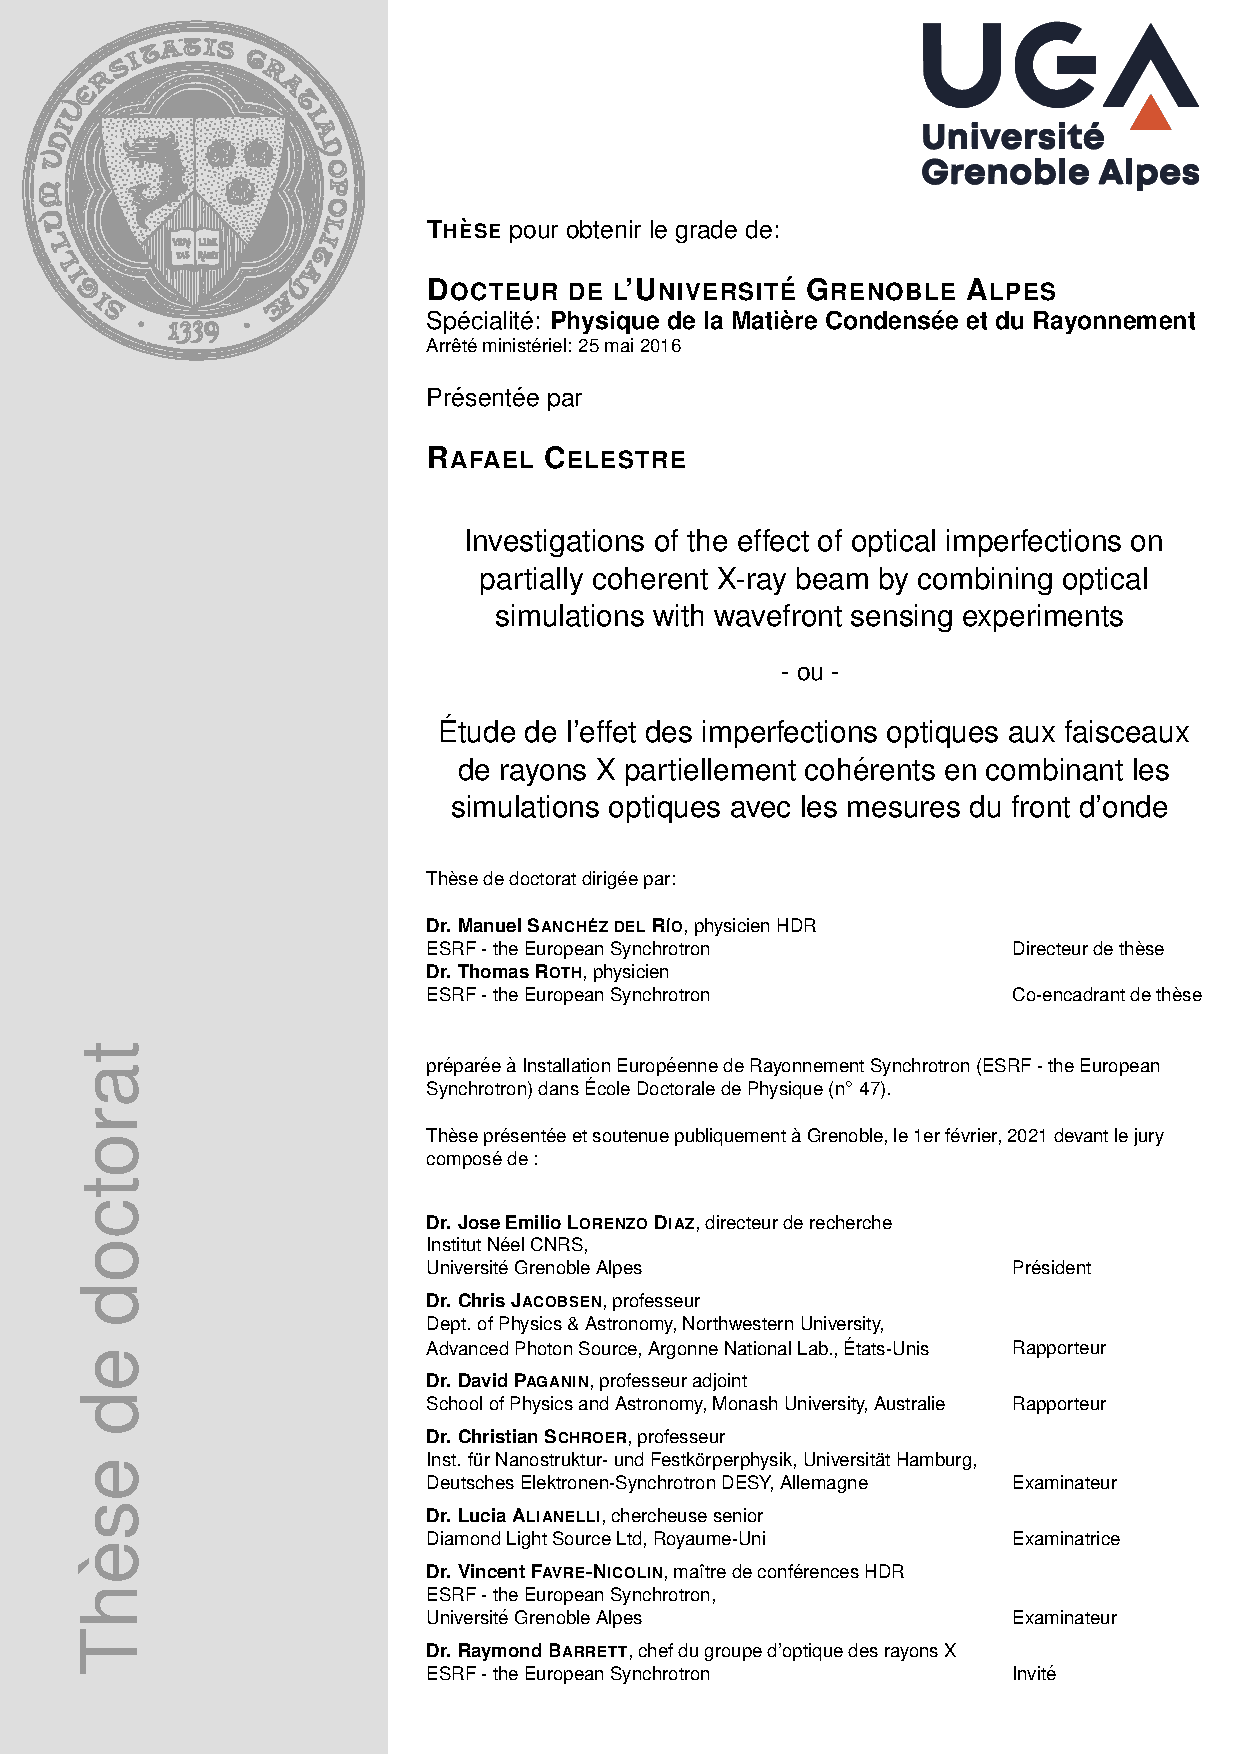
\includepdf[pages=-]{cover/cover.pdf}	
\end{titlepage}


% % ------------------------------------  --> lower title back for single page layout
% \hfill
% \vfill
% \begin{minipage}{9cm}

% {
% 	\small
% 	\textbf{\thesisName} \\
% 	\textit{\thesisTitle}
% 	\begin{center}
% 	- or - 
% 	\end{center}
% 	\textit{\thesisTitleFR} \\[1.5em]
% 	\textbf{Supervisor}: \thesisFirstSupervisor\\ 
% 	\thesisFirstSupervisorGroup\\
% 	\thesisFirstSupervisorDepartment\\
% 	\textbf{Co-supervisor}: \thesisSecondSupervisor\\
% 	\thesisSecondSupervisorGroup\\
% 	\thesisSecondSupervisorDepartment\\[1.5em]
% 	\textbf{\thesisUniversity} \\
% % 	\textit{\thesisUniversityGroup} \\
% % 	\thesisUniversityDepartment \\
% 	\thesisUniversityStreetAddress \\
% 	\thesisUniversityPostalCode\ - \thesisUniversityCity
% }
% \end{minipage}

		    % INCLUDE: all titlepages
\cleardoublepage
\pagestyle{plain}				% display just page numbers
% 13/11/2020 - First round of corrections: added Thomas & Ray corrections
\pdfbookmark[0]{Abstract}{Abstract}
\chapter*{Abstract}
\label{sec:abstractEN}
\vspace*{-10mm}

The advent of the 4$^{\text{th}}$ generation high-energy synchrotron facilities (ESRF-EBS and the planned APS-U, HEPS, PETRA-IV and SPring-8 II) and free-electron lasers (Eu-XFEL, SLAC) allied with the recent demonstration of high-quality free-form refractive optics for beam shaping and optical correction has reinforced interest in compound refractive lenses (CRLs) as optics for beam transport, probe formation in X-ray micro- and nano-analysis as well as for imaging applications. Within this context, in 2016, the ESRF resumed the fabrication and tests of 2D focusing bi-concave aluminium X-ray lenses. Current refractive optics, commercial or otherwise, have non-negligible aberrations which deteriorate their final performance and accurate modelling with input from metrology is necessary to evaluate the wavefront degradation and in order to propose mitigation strategies.

In physical optics, weakly focusing elements are usually simulated as a single thin element in the projection approximation. While a single X-ray lens at typical operation conditions can often be represented in this way, simulating a full CRL with a similar approach leads to an idealised model that lacks versatility. This work proposes decomposing a CRL into its lenslets separated by a free-space propagation, which resembles the multi-slicing techniques (MS) already used for optical simulations. Attention is given to modelling the single lens element by adding additional degrees of freedom allowing the modelling of typical misalignments and fabrication errors. Orthonormal polynomials for optical aberrations as well as at-wavelength metrology data are also used to obtain realistic simulation results, which are presented in several coherent- and partially-coherent simulations throughout this work. They compare qualitatively well with the experimental data and are used to evaluate the effect of optical imperfections on partially coherent X-ray beam and the suitability of common figures of merit. Unlike other works, the modelling presented here can be used transparently with one of the most popular codes for X-ray beamline design, "Synchrotron Radiation Workshop" (SRW), and is publicly available on GitLab.

Optical imperfections measured with high spatial resolution can be added to the MS representation of a CRL to accurately represent real X-ray lenses. X-ray speckle vector tracking (XSVT) is a versatile technique that conveniently obtains the figure errors of X-ray lenses in the projection approximation with high spatial resolution and is used in this work for characterising lenses to be used in the modelling presented here. This thesis presents a review of most relevant concepts of X-ray speckle based imaging applied to lens metrology.

Implementing the MS model of a CRL using metrology data allows extraction of the accumulated figure errors of stacked lenses and enables the calculation of phase corrections. Finally, this thesis presents a methodology for calculating the profile of refractive correctors, which is applied to produce phase plates ablated from diamond. Early experimental results show an improvement on the beam profile, but the transverse alignment of the phase-plate is a limiting factor. Further improvements to the metrology of lenses and correction plates and alignment protocols are necessary to optimise the performance of these optical correctors.
\cleardoublepage
\pagestyle{plain}				% display just page numbers
% 13/11/2020 - First round of corrections: added Thomas' corrections
\pdfbookmark[0]{Résumé}{Résumé}
\chapter*{Résumé}
\label{sec:abstractFR}
\vspace*{-10mm}

L'avènement des installations synchrotron à haute énergie de quatrième génération (ESRF-EBS et les projets APS-U, PETRA-IV et SPring-8 II) et des lasers à électrons libres (Eu-XFEL, SLAC), allié à la récente démonstration d'optiques réfractives à forme libre de haute qualité pour la mise en forme des faisceaux et la correction optique, a ravivé l'intérêt pour les lentilles réfractives composées (LRC) en tant qu'optiques pour le transport des faisceaux, la formation de sondes dans la micro- et la nano-analyse des rayons X ainsi que pour les applications d'imagerie. Dans ce contexte, en 2018, l'ESRF a repris la fabrication et les essais de lentilles biconcaves à rayons X en aluminium à focalisation 2D. Les optiques réfractives actuelles, commerciales ou autres, présentent des aberrations non négligeables qui détériorent leurs performances finales et une modélisation précise avec l'aide de la métrologie est nécessaire pour évaluer la dégradation du front d'onde et proposer des stratégies d'atténuation.

En optique physique, les éléments faiblement focalisants sont généralement simulés comme un seul élément mince dans l'approximation de projection. Alors qu'une seule lentille à rayons X dans des conditions de fonctionnement typiques peut souvent être représentée de cette manière, la simulation d'un LRC complet avec une approche similaire conduit à un modèle idéalisé qui manque de polyvalence. Ce travail propose de décomposer un LRC en ses petites lentilles séparées par une propagation en espace libre, ce qui ressemble aux techniques de découpage multiple (MS) déjà utilisées pour les simulations optiques. L'attention est portée sur la modélisation de l'élément à lentille unique en lui ajoutant des degrés de liberté supplémentaires permettant la modélisation des désalignements typiques et des erreurs de fabrication. Des polynômes orthonormaux pour les aberrations optiques ainsi que des données de métrologie en rayons X sont également utilisés pour obtenir des résultats de simulation réalistes, qui sont présentés dans plusieurs simulations cohérentes et partiellement cohérentes tout au long de ce travail. Ils se comparent qualitativement bien avec les données expérimentales et sont utilisés pour évaluer l'effet des imperfections optiques sur la dégradation du faisceau de rayons X partiellement cohérent et la pertinence des figures de mérite communes. Contrairement à d'autres travaux, la modélisation présentée ici peut être utilisée de manière transparente avec l'un des codes les plus populaires pour la conception de lignes de faisceaux de rayons X, "Synchrotron Radiation Workshop" (SRW), et est disponible sur GitLab.

Les imperfections optiques mesurées avec une haute résolution spatiale peuvent être ajoutées à la représentation MS d'un LRC pour représenter avec précision de véritables lentilles à rayons X. Le suivi vectoriel du speckle des rayons X (XSVT) est une technique polyvalente qui permet d'obtenir facilement les erreurs de figure des lentilles de rayons X dans l'approximation de projection avec une haute résolution spatiale et est utilisée dans ce travail pour caractériser les lentilles 2D-beryllium qui sont ensuite utilisées dans les modélisations présentées ici. Cette thèse présente une revue des concepts les plus pertinents de l'imagerie basée sur le speckle des rayons X appliquée à la métrologie des lentilles.

La mise en œuvre du modèle MS d'un LRC en utilisant des données de métrologie permet d'extraire les erreurs cumulées des lentilles empilées et permet le calcul des corrections de phase. Cette thèse se termine par la présentation d'une méthodologie de calcul du profil des correcteurs de réfraction, qui est appliquée pour produire des plaques de phase ablatées au diamant. Les premiers résultats expérimentaux montrent une amélioration du profil du faisceau, mais l'alignement transversal de la plaque est un facteur limitant. D'autres améliorations de la métrologie des lentilles et des plaques de correction, des efforts dans la délimitation des protocoles d'alignement sont nécessaires pour amener la conception des correcteurs optiques dans l'ESRF.
\cleardoublepage
\pagestyle{plain}				% display just page numbers

\pdfbookmark[0]{Acknowledgement}{Acknowledgement}
\chapter*{Acknowledgement}
\label{sec:acknowledgement}
\vspace*{-10mm}

Acknowledgement

% I do not really know when I discovered I wanted to have a career in science. It could have been one of the many Saturdays my mother brought me to her lab to "play with the microscopes" while she had to work, the numerous science kits my dad got me when I was little or that time in 1995 I dressed up as a "crazy scientist" for carnaval in Brazil. But as long as I can remember, I wanted to be a lumberjack, I mean, a physicist. 
    % INCLUDE: acknowledgement
\cleardoublepage

\setcounter{tocdepth}{4}		% define depth of toc
\setcounter{secnumdepth}{2}

% dirty solution to hyperlink unnumbered sections: \hyperlink{sec:name}{Real name... create balloon for keeping tabs on names?}
% this should be used with: \addcontentsline{toc}{subsubsection}{The subsubsection name}
% 

\tableofcontents				% display table of contents
\cleardoublepage

\listoffigures
\cleardoublepage

\listoftables
\cleardoublepage

% --------------------------
% Body matter
% --------------------------
\pagenumbering{arabic}			% arabic page numbering
\setcounter{page}{1}			% set page counter
\pagestyle{maincontentstyle} 	% fancy header and footer

\chapter*{Foreword}\addcontentsline{toc}{chapter}{Foreword}


\section*{Motivation}\addcontentsline{toc}{section}{Motivation}


% Explain the context of the ESRF-EBS upgrade, the renaissance of refractive optics and the resume of Al lens production. 

\section*{Objectives}\addcontentsline{toc}{section}{Objectives}


\section*{Outline}\addcontentsline{toc}{section}{Outline}

This work is divided into five chapters and one appendix with the relevant publications from the time as a PhD candidate. This work is organised as follows:
\\
\\
\textbf{Chapter \ref{sec:x-rays}~-~\nameref{sec:x-rays}} is the first of two theoretical chapters, presents ...
\\
\\
\textbf{Chapter \ref{sec:x-ray_optics}~-~\nameref{sec:x-ray_optics}}: introduces ... this chapter concludes the presentation of the theoretical aspects necessary for this dissertation.
\\
\\
\textbf{Chapter \ref{sec:optical_imperfections}~-~\nameref{sec:optical_imperfections}} introduces ...
\\
\\
\textbf{Chapter \ref{sec:effect_optical_imperfections}~-~\nameref{sec:effect_optical_imperfections}} introduces ...
\\
\\
\textbf{Chapter \ref{sec:conclusion}~-~\nameref{sec:conclusion}}  ...$\blacksquare$ \cleardoublepage
% 09/11/2020 - First round of corrections: added Paganin, Thomas and Manolo's corrections
\begin{refsection}

%-------------------------------------------------------------------------
%-------------------------------------------------------------------------
\chapter{On a new kind of rays}\label{sec:x-rays}
%-------------------------------------------------------------------------
%-------------------------------------------------------------------------


Hard X-rays are electromagnetic radiation with wavelength below\footnote{The choice of wavelength or energy to limit soft-, tender- and hard- X-rays is rather arbitrary. The conversion of energy to wavelength in practical unities is usually one by as $\text{E}(\text{keV})=12.3984/\lambda(\text{\r{A}})$} 2~\r{A}. From their discovery in 1895 by W. C. R\"{o}ntgen [\cite{Roentgen1896}], the first observation of synchrotron radiation (SR) in 1947 [\cite{Elder1947}], the first (late 1950's and early 1960's), second (late 1970's and early 1980's), third (end of 1980's and early 1990's) and the fourth generation (late 2000's and early 2010's) of accelerator-based X-ray sources, the brilliance and consequently, the coherent fraction has increased out-passing the Moore's law [\cite{Robinson2015}]. This chapter is dived into three main parts. The first part introduces the concept of brilliance and connects it to the coherent fraction of synchrotron radiation emission, presenting undulators as the mains source of coherent X-rays in a synchrotron radiation facilities. In the second part of this chapter, the scalar wave theory is presented as a framework for modelling X-ray propagation through free-space and optical elements. Some definitions regarding optical coherence are also presented. The last part of this chapter deals with simulation strategies based on the degree of spatial coherence of the radiation.
%-------------------------------------------------------------------------
%-------------------------------------------------------------------------
\section{From the Hittorf's tube to the EBS}\label{sec:sources_intro}
%-------------------------------------------------------------------------
%-------------------------------------------------------------------------
Since the discovery\footnote{Professor W. C. R\"{o}ntgen has published his first notes on the discovery of X-rays in January 1896 in [\cite{Roentgen1896}]. In March the same year, R\"{o}ntgen went on to publish some additional notes on his discovery [\cite{Roentgen1896a}]. Further observations of the X-ray properties were later published in [\cite{Roentgen1897}].} of X-rays in late November 1895 by W. C. R\"{o}ntgen [\cite{Roentgen1896}] up to the concept and implementation of the fourth generation high-energy synchrotron light sources in the second half of the 2010's [\cite{Eriksson2016}], there has been an Herculean amount of work directed to increasing a key energy-dependent quality parameter of x-ray sources, called brilliance\footnote{Although a common jargon in X-ray science and technology, the term brilliance is not unanimously agreed upon. For an insightful discussion on the terminology, please refer to the discussion in [\cite{Mills2005}] and to the Chapter~3.9 and Table~3.1 in [\cite{Talman2006}]. Eq.~\ref{eq:brilliance} is an approximation result. For an accurate calculation of the brilliance, please, refer to [\cite{Walker2019}].}:
\begin{equation}\label{eq:brilliance}
   \mathcal{B}_0 = \frac{\varphi}{4\pi^2\epsilon_\mathrm{h}\epsilon_\mathrm{v}},
\end{equation}{}
where $\varphi$ is the X-ray photon flux for a given bandwidth $\Delta\mathrm{E}/\mathrm{E}=0.001$ centred at energy E,  given in $(\mathrm{photons}/\mathrm{s}/0.1\%\mathrm{bw.})$. Both $\epsilon_\mathrm{h}$ and $\epsilon_\mathrm{v}$ refer to the photon-beam emittances in the horizontal and vertical planes, respectively. The photon beam emittance is defined as:
\begin{equation}
    \epsilon_{\mathrm{h,v}}\equiv\Sigma_{\mathrm{h,v}}\cdot\Sigma_{\mathrm{h,v}}'.
\end{equation}{}
Here $\Sigma_{\mathrm{h,v}}$ stands for the beam size and $\Sigma'_{\mathrm{h,v}}$ is the photon-beam divergence. The usual unit used for the beam size is $(\mathrm{mm})$ and for beam divergence is $(\mathrm{mrad})$, hence brilliance is commonly given in $(\mathrm{ph}/\mathrm{s}/0.1\%\mathrm{bw.}/\mathrm{mm}^2/\mathrm{mrad}^2)$ [\cite{Kim1986}]. It is clear from Eq.~\ref{eq:brilliance} that increasing the brilliance means increasing the spectral photon flux $\varphi$ and/or reducing the photon-beam emittance in both horizontal and vertical directions ($\epsilon_\mathrm{h}$ and $\epsilon_\mathrm{v}$), i.e. having a smaller and more collimated X-ray source.
%-------------------------------------------------------------------------
%-------------------------------------------------------------------------
\subsection{X-ray sources}\label{sec:sources}
%-------------------------------------------------------------------------
%-------------------------------------------------------------------------
Two main processes are responsible for generating X-rays: acceleration of charged particles, in particular, electrons; and the change of an electron state from a higher atomic or ionic energy level to a lower one.

In the very early X-ray sources\footnote{This works focuses only on artificial X-ray sources, most specifically storage-rings. X-rays and synchrotron radiation also occur in nature with astrophysical sources of synchrotron radiation, which exist across the full electromagnetic spectrum, being of extremely scientific relevance [\cite{Ginzburg1965,Wielebinski2006}].} such as the Hittorf's tube used by R\"{o}ntgen\footnote{On the opening sentence of his most important work \textit{"On a new kind of rays"}, R\"{o}ntgen mentions that X-rays can be produced by [sic.] \textit{"an electric discharge passing through a Hittorf's tube or a well-exhausted Lenard's or Crook's tube"} [\cite{Roentgen1896}].} or any modern X-ray tube (electron-impact X-ray sources) both processes generate X-rays: Bremsstrahlung by rapid deceleration of fast electrons, generating a broad-band smooth spectrum; and characteristic radiation (X-ray fluorescence), responsible for narrow spikes in the spectrum. Although modern sources can focus the electron-beam into the target (anode), reducing the source size considerably, the emission of X-rays happens in a large solid angle, $2\pi~(\mathrm{steradians})$. The emission angle, in conjunction with the fact that the X-ray flux is limited by the low current of electrons, makes X-ray tubes very-low brilliance sources  [\cite[\textit{§1.6} \& \textit{§2}]{Michette1993}].

\begin{figure}[t]
    \centering
    {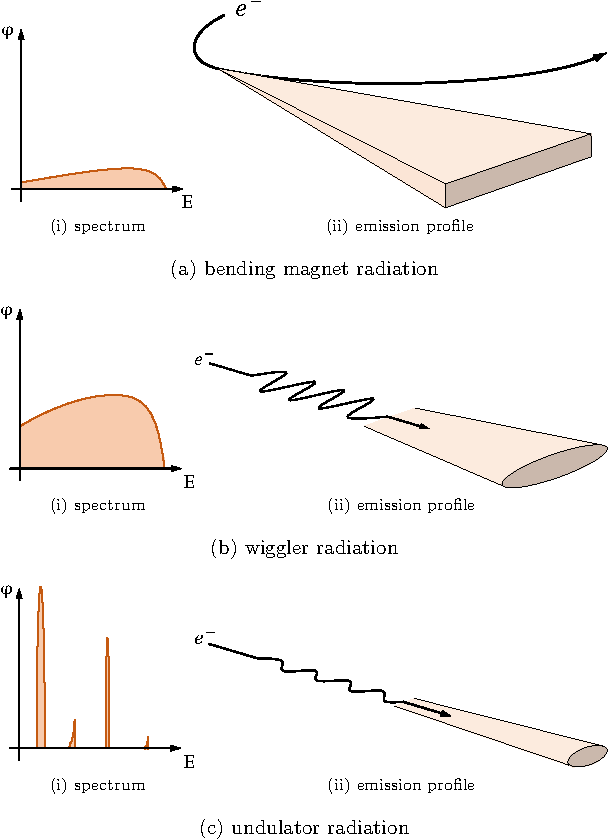
\includegraphics[width=.55\linewidth]{figures/ch02/x-ray_sources.pdf}}
    \caption[Synchrotron radiation emission]{Sketch of the three main sources of synchrotron radiation. On the left-handed side the photon-flux $\varphi$ as a function of energy $\mathrm{E}$ is shown. The right-hand side shows the electron ($e^-$) trajectory and the accompanying emission profile. Figure adapted from Figs.~5.1-5.3 in [\cite{Attwood1999}] and Fig.~1.2 from [\cite{Clarke2004}].}
    \label{fig:emission}
\end{figure}

In accelerator-based X-ray sources, more specifically, storage-ring-like facilities\footnote{Linear accelerators are also used as a source of intense synchrotron radiation, in particular in free-electron lasers (XFELs) [\cite{Huang2007}].}, (ultra-relativistic\footnote{At an energy of $\sim$11.43~MeV, the electron reaches $v/c = 99.9\%$ and at roughly 36.13~MeV the ratio is $v/c = 99.99\%$, where $v$ is the particle velocity and $c$ is the speed of light. Storage rings dedicated to synchrotron radiation operate at least above a few hundred MeV.}) electrons are usually chosen for generating X-rays as their low rest mass means that they emit by far the most radiation for a given particle energy. Charged particles in storage rings are subjected to a magnetic field perpendicular to the direction of motion and this causes the particle to move in a circular trajectory (centripetal acceleration). If the particle is non-relativistically accelerated, the emitted radiation is described by the Larmor pattern (torus-shaped profile), which shows no radiation in the direction of acceleration. However, for a particle in the ultra-relativistic regime, the Lorentz-transformed radiation pattern shows that the (synchrotron) radiation pattern is very peaked in the forward direction with a narrow angular divergence (cf. Fig.~\ref{fig:emission}) [\cite{Jackson1998}].

There are two main families of X-ray sources in a synchrotron facility: bending magnets (BM's) and insertion devices (IDs). Bending magnets are necessary magnetic structures in the storage ring to deflect the electron-beam transversely to its motion direction and keep it in a closed trajectory by applying a constant magnetic field or gradient. They produce a smooth broad-band spectrum and the photon-beam footprint is very large as both the source and divergence\footnote{The typical emission angle of synchrotron radiation is given by $1/\gamma$, where $\gamma$ is the Lorentz factor. For an electron in a storage ring: $\gamma=1957\cdot\mathrm{E(GeV)}$, with $\mathrm{E(GeV)}$ being the electron energy [\cite[\textit{§2.2.1}]{Als-Nielsen2011}].} sizes are very large. Historically, BMs have been used as the primary source of X-rays in first- and second-generation light-sources\footnote{The first generation of synchrotron light sources is usually attributed to the parasitic use of high-energy physics accelerators. The second-generation marks the beginning of fully-dedicated machines for synchrotron radiation.}. The bending magnet radiation spectrum and profile are shown in Fig.~\ref{fig:emission}(a)~and~(b). Storage rings are a multi-edge polygon where at each vertex sits a bending magnet gently deflecting the electron-beam keeping the electrons in a closed loop. The distance between two adjacent dipole magnets is called a straight section and is where insertion devices are placed.

Insertion devices (IDs) are periodic magnetic structures that sinusoidally deflect the electron-beam transversely to its direction of motion. IDs can be sub-grouped into two categories based on the amplitude of the electron motion inside them and their magnetic period: wigglers have a higher magnetic field applied to the electron-beam causing the amplitude of electron motion to be large. The magnetic period in a wiggler is considered to be large. This generates a broad-band spectrum several times more intense than that of a bending magnet (higher flux) - wigglers are also called wavelength shifters. The beam footprint is also very large: the source size is big and the beam has a higher divergence than that of the natural divergence of synchrotron radiation from BM's. Figures~\ref{fig:emission}(b) shows the spectrum and emission profile of a wiggler insertion device. The second member of the ID family is the undulator. In it, the amplitude of the electron motion is much smaller than inside a wiggler. This is because in the undulators a less intense magnetic field is applied to the electrons and due to the fact that the magnetic period is usually smaller than the one of a wiggler. The small excursion of the electrons inside the undulator accounts for a small photon source size with low divergence. Due to the low electron-motion amplitude, constructive interference between the emitted radiation occurs and the spectrum of an undulator is composed of narrow-band peaks called undulator harmonics\footnote{If the observer is on-axis with the electron motion, only odd harmonics are observed. Away from the emission axis, even harmonics start being observed [\cite[\textit{§4.2}]{Clarke2004}].}. This is possible because in an undulator, the electron excursion is smaller than the X-ray cone emission. Figure~\ref{fig:emission}(c) shows the spectrum and emission profile of an undulator. The advent of storage rings specially designed to accommodate ID's marks the third generation of synchrotron light sources, from which the ESRF - European Synchrotron Research Facility (1994) in France is the pioneering machine, followed by the APS - Advanced Photon Source (1996) in the USA and the SPring-8 - Super Photon ring-8~GeV (1999) in Japan. 

%-------------------------------------------------------------------------
%-------------------------------------------------------------------------
\subsection{High brilliance X-ray sources}\label{sec:brilliance}
%-------------------------------------------------------------------------
%-------------------------------------------------------------------------

The small photon source size and low divergence of the X-rays emitted by an undulator make it a great candidate for generating high-brilliance X-ray beams. As Eq.~\ref{eq:brilliance} suggests, increasing the brilliance can be done by two different strategies: increasing the photon flux, which is done by increasing the electron current in the storage ring; and/or by reducing the photon-beam emittance.

The radiation profile (beam sizes and divergences) emitted by an undulator is given by the convolution between electron-beam profile and the radiation pattern specific of the X-ray source\footnote{This is true for any accelerator-based X-ray source - cf. chapter "3.10 - Photon beam features inherited from the electron beam" in [\cite{Talman2006}].}: 
\begin{subequations}\label{eq:undulator}
    \begin{align}   
    \Sigma_{\mathrm{h,v}} &= \sigma_{e_{\mathrm{h,v}}}*\sigma_{u_{\mathrm{h,v}}},\\
    \Sigma'_{\mathrm{h,v}} &= \sigma'_{e_{\mathrm{h,v}}}*\sigma'_{u_{\mathrm{h,v}}}.
    \end{align}
\end{subequations}{}
Here $\Sigma_{\mathrm{h,v}}$ and $\Sigma'_{\mathrm{h,v}}$ are the already defined photon-beam size and divergence. The $\sigma_{e_{\mathrm{h,v}}}$ and $\sigma'_{e_{\mathrm{h,v}}}$ represent the electron-beam size and divergence. Lastly, $\sigma_{u_{\mathrm{h,v}}}$ and $\sigma'_{u_{\mathrm{h,v}}}$ are the specific radiation pattern size and divergence of the insertion device - these are the obtained by calculating the emission of a filament electron-beam (negligible dimension and divergence) passing through the magnetic field of the insertion device. Once designed, the specific radiation pattern of an undulator\footnote{The specific radiation pattern of an undulator is a function of its magnetic period, number of periods, magnetic field, storage ring energy and X-ray emission-wavelength.} is considered to be a fundamental wavelength-dependent property of the insertion device\footnote{In the literature, there is variety of formulae for calculating the specific radiation pattern size and divergence [\cite{Kim1986, Kim1989, Tanaka2009, Elleaume2013}]. Different assumptions, approximations and fits are done on their derivation. It is important to state that those are approximations and should not be regarded as fundamental results - please, refer to the discussion in [\cite{Walker2019}]. The exact calculation of the radiation pattern can be done by computing the electric field of an electron subjected to an arbitrary magnetic field - cf. [\cite{Chubar1995, Chubar2001}] or by calculating the Wigner-function for synchrotron radiation [\cite{Bazarov2012}] as in [\cite{Tanaka2014}]. \label{note:und_prof}}.

A closer look into Eqs.~\ref{eq:undulator} allows one to suppose three distinct regimes for the photon-beam characteristics: a) $\epsilon_{e_{\mathrm{h,v}}}\gg\epsilon_{u_{\mathrm{h,v}}}$ in this regime, the photon-beam characteristics are dominated by the electron-beam, which is well approximated by a Gaussian distribution. This is usually the case for horizontal emittance in third-generation synchrotrons; b) an intermediate state where the electron-beam emittance $\epsilon_{e_{\mathrm{h,v}}}$ is comparable to $\epsilon_{u_{\mathrm{h,v}}}$ leading to a photon-beam profile with clear contributions of both the electron-beam and specific radiation pattern of the undulator; c) the electron-beam emittance can be further reduced so that $\epsilon_{e_{\mathrm{h,v}}}\ll\epsilon_{u_{\mathrm{h,v}}}$ and the photon-beam profile is dominated by the undulator's specific radiation pattern. Since $\epsilon_{u_{\mathrm{h,v}}}$ is a fundamental limit, efforts to reducing the electron-beam beyond that limit will not have any impact in the photon-beam profile. Mathematically, the three emittance regimes can be expressed as:
\begin{subequations}\label{eq:emittances}
    \begin{align}
           \epsilon_{\mathrm{h,v}}&\Big\vert_{\epsilon_{e_{\mathrm{h,v}}}\gg\epsilon_{u_{\mathrm{h,v}}}}  \simeq\Big(\sigma_{e_{\mathrm{h,v}}}*\delta_{u_{\mathrm{h,v}}}\Big)\Big(\sigma'_{e_{\mathrm{h,v}}}*\delta_{u_{\mathrm{h,v}}}\Big)=\sigma_{e_{\mathrm{h,v}}}\sigma'_{e_{\mathrm{h,v}}},\\
           \epsilon_{\mathrm{h,v}}&\Big\vert_{\epsilon_{e_{\mathrm{h,v}}}\sim\epsilon_{u_{\mathrm{h,v}}}}
           \simeq\Big(\sigma_{e_{\mathrm{h,v}}}*\sigma_{u_{\mathrm{h,v}}}\Big)\Big(\sigma'_{e_{\mathrm{h,v}}}*\sigma'_{u_{\mathrm{h,v}}}\Big)=\Sigma_{\mathrm{h,v}}\Sigma'_{\mathrm{h,v}},\\
           \epsilon_{\mathrm{h,v}}&\Big\vert_{\epsilon_{e_{\mathrm{h,v}}}\ll\epsilon_{u_{\mathrm{h,v}}}}
           \simeq \Big(\delta_{e_{\mathrm{h,v}}}*\sigma_{u_{\mathrm{h,v}}}\Big)\Big(\delta_{e_{\mathrm{h,v}}}*\sigma'_{u_{\mathrm{h,v}}}\Big)=\sigma_{u_{\mathrm{h,v}}}\sigma'_{u_{\mathrm{h,v}}}.
    \end{align}
\end{subequations}{}
Where $\delta$ represents the Dirac function. The electron-beam emittance matching to the undulator's specific radiation pattern is shown in Fig.~\ref{fig:matching}. Fourth-generation synchrotron storage-ring-based light-sources\footnote{The fourth generation synchrotron light sources or ultra-low emittance machines have been proposed as early as the 1990's [\cite{Einfeld1996, Einfeld2014}], but were deemed to be technologically unfeasible for high-energy storage rings [\cite{Ropert2000, Elleaume2003}]. Overcoming the technological barriers [\cite{Borland2014}] was essential in paving the way for high energy storage rings with ultra-low emittance [\cite{Bei2010, Eriksson2016}]. The first machines to come online using the multi-bend-achromat design (MBA) are the MAX-IV in Sweden (2016) and the SIRIUS in Brazil (2019) - the former operating with two storage rings: $1.5~\mathrm{GeV}$ and $3~\mathrm{GeV}$ and the latter operating at $3~\mathrm{GeV}$. The ESRF upgrade programme has opted for a hybrid-multi-bend-achromat (HMBA) magnetic lattice for its new storage ring [\cite{Biasci2014}] and it is the first of its kind to operate at high-energies ($6~\mathrm{GeV}$). The lattice concept behind the Extremely Brilliant Source (ESRF-EBS) has it's origins in 2006 with the SuperB project for an electron-positron collider [\cite{Raimondi2017}] and in early 2020 has produced the first X-rays.} use emittance-matching - Eq.~\ref{eq:emittances}(b) mainly, but ideally Eq.~\ref{eq:emittances}(c) - as the main source of increasing the X-ray brightness\footnote{This is due to the fact that with the new storage-ring designs (multi-bend-achromat and its variations), the electron-beam emittance can be routinely reduced one to two orders of magnitude, when compared to current third-generation light sources. To obtain equivalent gain in brightness by just increasing the electron-beam current is very challenging in function of collective effects (coherent and incoherent). On the top of that, there are thermal load issues on the vacuum system and on the beamline optics, that is, the X-ray transport system to the sample. This footnote is the result of discussions with Pedro F. Tavares (MAX-IV, Sweden)  and Boaz Nash (RadiaSoft LLC, USA).} [\cite[\textit{§21.8.1}]{Wiedemann2015}].

\begin{figure}[t]
    \centering
    {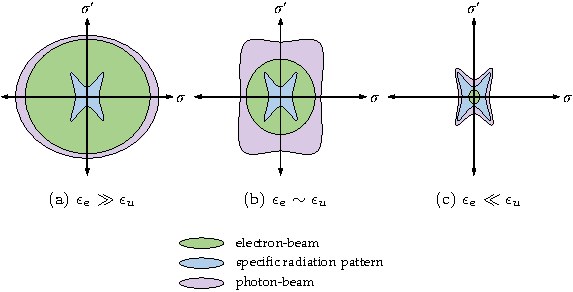
\includegraphics[width=.6\linewidth]{figures/ch02/emittance.pdf}}
    \caption[Emittance matching]{Matching of the electron-beam emittance to the undulator specific radiation pattern to increase the photon-beam brightness, where $\sigma$ stands for beam size and $\sigma'$ for beam divergence. Adapted from Fig.~21.20 in [\cite{Wiedemann2015}].}
    \label{fig:matching}
\end{figure}

%-------------------------------------------------------------------------
%-------------------------------------------------------------------------
\subsection{Undulators as a primary source of coherent X-rays}\label{sec:undulators}
%-------------------------------------------------------------------------
%-------------------------------------------------------------------------

 Let's consider the case of a filament electron-beam passing through a planar undulator. The associated emission at a resonant photon energy is symmetric and $\sigma_{u_{\mathrm{h}}}=\sigma_{u_{\mathrm{v}}}=\sigma_{u}$ and $\sigma'_{u_{\mathrm{h}}}=\sigma'_{u_{\mathrm{v}}}=\sigma'_{u}$ [\cite{Kim1989}]. Because the electron bunch has negligible emittance $\epsilon_e$ in both horizontal and vertical directions, the photon-beam emittance is given by $\epsilon_\mathrm{h,v}=\sigma_{u}\sigma'_u=\epsilon_\mathrm{u}$. The associated brilliance of such a filament beam is given by:
\begin{equation}\label{eq:brilliance_coherent}
\mathcal{B}_0 = \frac{\varphi}{4\pi^2\epsilon^2_{u}}
\end{equation}{}
Since the emission of a filament electron-beam is fully-coherent, it makes sense to define a coherent photon flux of a zero-electron-emittance-beam. From Eq.~\ref{eq:brilliance_coherent}:
\begin{equation}\label{eq:coherent_flux}
\varphi_\mathrm{coh.} = 4\pi^2\epsilon^2_{u}\mathcal{B}_0=\Bigg(\frac{\lambda}{2}\Bigg)^2\mathcal{B}_0.
\end{equation}{}
It is important to mention that the right-hand side of Eq.~\ref{eq:coherent_flux} is valid for any symmetric electric field distribution at any value of undulator detuning and it does not depend on a Gaussian approximation of the undulator specific radiation pattern [\cite{Walker2019}]. Although Eq.~\ref{eq:coherent_flux} implies that $\epsilon_u = \sigma_u\sigma'_u =\lambda/4\pi$, it has been demonstrated that the non-Gaussian behaviour of the undulator emission makes the photon-beam emittance approach asymptotically $\lambda/2\pi$ instead [\cite{Elleaume2013,Tanaka2009}]. One can define the coherent fraction as the ratio between the coherent flux $\varphi_\mathrm{coh.}$ (Eq.~\ref{eq:coherent_flux}) and the nominal photon-flux $\varphi = 4\pi^2\epsilon_\mathrm{h}\epsilon_\mathrm{v}\mathcal{B}_0$ (Eq.~\ref{eq:brilliance}):
\begin{equation}\label{eq:coherent_fraction}
\zeta =  \frac{\varphi_\mathrm{coh.}}{\varphi}=\frac{\epsilon^2_{u}}{\epsilon_\mathrm{h}\epsilon_\mathrm{v}}.
\end{equation}{}
Eq.~\ref{eq:coherent_fraction} allows to deduce that by reducing the electron-beam emittance, the coherence fraction is increased (cf. Eqs.~\ref{eq:emittances}). An important conclusion to be drawn is that emittance-matching as a form of increasing the photon-beam brilliance in fourth-generation synchrotrons increases the X-ray beam transverse (spatial) coherence\footnote{Please, refer to §\ref{sec:optical_coherence}~-~\textit{\nameref{sec:optical_coherence}} for a definition of spatial and temporal coherence.\label{note:coherence}}.

%-------------------------------------------------------------------------
%-------------------------------------------------------------------------
\subsubsection*{Temporal Coherence}
%-------------------------------------------------------------------------
%-------------------------------------------------------------------------

Lastly, the temporal coherence\footnote{See footnote \ref{note:coherence}.} of the synchrotron radiation emitted by storage rings should be addressed. Without further conditioning, the radiation emitted on the X-ray region exhibits low temporal coherence for high energies. Spectral filtering with monochromators increases the temporal coherence at the expense of photon-flux reduction. Compressing the electron bunch length also offers an increased temporal coherence for X-rays, as coherent synchrotron radiation (CSR) naturally appears when the electron-beam bunch length is comparable to the observed radiation wavelength - cf. [\cite{Chubar2006}], [\cite[\textit{§3.8} \& \textit{§13}]{Talman2006}] and [\cite[\textit{§21.7}]{Wiedemann2015}]. 

%-------------------------------------------------------------------------
%-------------------------------------------------------------------------
\subsection*{Recommended literature}
%-------------------------------------------------------------------------
%-------------------------------------------------------------------------

The correct description of the electron-beam inside each different source of X-rays in a storage ring is of primary importance for accurate modelling of the radiation spectrum and photon spatial distribution, with consequences to X-ray optical design.
An extensive review on particle accelerator physics is given by [\cite{Duke2000}] and by [\cite{Wiedemann2015}]. An in-depth look into X-rays from accelerator sources can be found in [\cite{Clarke2004}], in [\cite{Talman2006}] and in [\cite{Elleaume2013}].

The accurate calculation of the brightness from undulators in low-emittance accelerators and the coherence properties of the X-rays from them emitted is a vivid topic and a deeper look into it is offered by [\cite{Bazarov2012, Tanaka2014, Geloni2015, Geloni2008, Walker2019, Khubbutdinov2019}]. See also [\cite{Singer2014}].

\section{Physical optics}\label{sec:physical_optics}
\begin{figure}[t]
    \centering
    {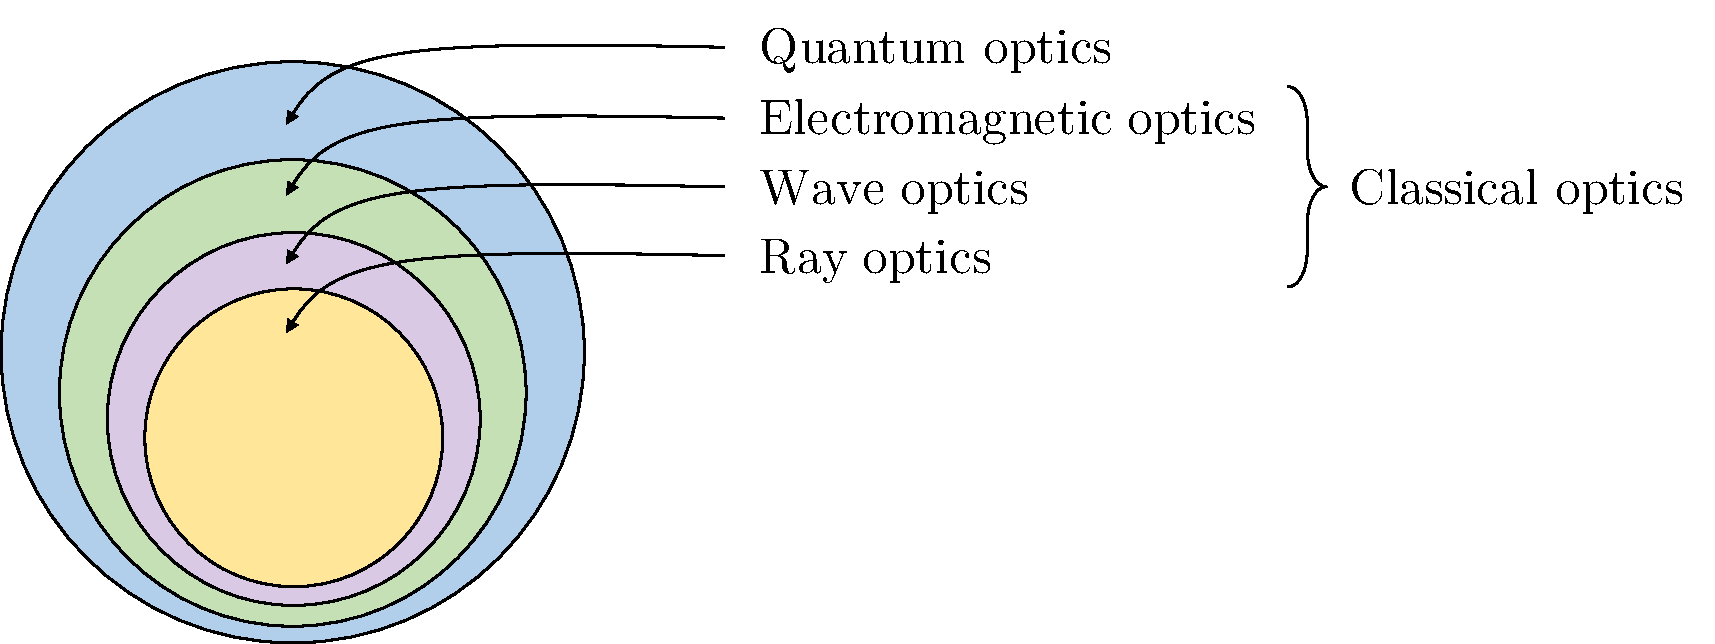
\includegraphics[width=.55\linewidth]{figures/ch02/optics.pdf}}
    \caption[Hierarchical optical theories]{Hierarchical optical theories. Optical modelling in the X-ray regime can be accurately represented in the realms of wave optics for most cases where coherence effects are present. Adapted from Fig.~1.0-1 in [\cite{Saleh2019}].}
    \label{fig:optical_theories}
\end{figure}
The increasing coherent fraction of X-rays from fourth-generation storage rings requires
an appropriate framework for their representation. Light can be described by an electromagnetic wave phenomenon governed by the Maxwell equations - cf. [\cite[\textit{§1.1}]{born_wolf1999}]:
\begin{subequations}\label{eq:Maxwell}
    \begin{align}
        \nabla\cdot\textbf{E} &= \frac{\rho}{\varepsilon}
                                       &&(\small{\text{Gau{\ss}'s~law}}),\\
        \nabla\cdot\textbf{B} &= 0 
                                       &&(\small{\text{Gau{\ss}'s law for magnetism}}),\\
        \nabla\times\textbf{E} &= -\frac{\partial}{\partial t}\textbf{B}
                                        &&(\small{\text{Faraday's law}}),\\
        \nabla\times\textbf{B} &= \mu\Bigg(\textbf{J}+\varepsilon\frac{\partial}{\partial t}\textbf{E}\Bigg)
                                       &&(\small{\text{Ampère's law modified by Maxwell}}).
    \end{align}
\end{subequations}{}
Where $\textbf{E}\equiv\textbf{E}(x,y,z,t)$ is the electric field, $\textbf{B}\equiv\textbf{B}(x,y,z,t)$ is the magnetic induction, $\varepsilon\equiv\varepsilon(x,y,z,t)$ and $\mu\equiv\mu(x,y,z,t)$ are the electric permittivity and magnetic permeability, $\rho\equiv\rho(x,y,z,t)$ is the charge density and $\textbf{J}\equiv\textbf{J}(x,y,z,t)$ is the current density. The operator $\nabla\cdot\bullet$ denotes the divergence of a vectorial field (scalar function) and $\nabla\times\bullet$ is the curl operator (vectorial function), where $\bullet$ is a generic vectorial field. The Cartesian coordinates $(x,y,z)$ and time $t$ have been omitted in favour of a more compact notation. Although electromagnetic optics provides the most complete framework for classical optical phenomena, it is possible to move away from the vectorial treatment of light towards a scalar wave theory in order treat a large variety of relevant optical phenomena. This simplified treatment of light is commonly referred to scalar wave optics or physical optics (cf. Fig.~\ref{fig:optical_theories} for the hierarchical representaion of optical theories). X-ray wave-fields in free-space are discussed in §\ref{sec:free-space}~-~\textit{\nameref{sec:free-space}} and their transmission through generic refractive optical elements is discussed in §\ref{sec:thin_element}~-~\textit{\nameref{sec:thin_element}}.

%-------------------------------------------------------------------------
%-------------------------------------------------------------------------
\subsection{Free-space propagation}\label{sec:free-space}
%-------------------------------------------------------------------------
%-------------------------------------------------------------------------

In order to describe wave-fields in free-space under the scalar theory, one usually starts\footnote{The developments in §\ref{sec:free-space}~-~\textit{\nameref{sec:free-space}} are inspired by the derivations from [\cite[\textit{§1}]{Paganin2006}] and [\cite[\textit{§3} \& \textit{§4}]{Goodman2017}].} by obtaining the Maxwell equations for free-space (vacuum). This is done considering that the medium where the wave-fields exist are uncharged and non-conducting, which is done by letting $\rho=0$ and $\textbf{J}=\textbf{0}$ in Eqs.~\ref{eq:Maxwell}a and~\ref{eq:Maxwell}d:
\begin{subequations}\label{eq:Maxwell_free}
    \begin{align}
        \nabla\cdot\textbf{E} &= \textbf{0},\\
        \nabla\times\textbf{B} &= \mu_0\varepsilon_0\frac{\partial}{\partial t}\textbf{E}.
    \end{align}
\end{subequations}{}
Where $\varepsilon_0$ and $\mu_0$ are the vacuum electric permittivity and magnetic permeability. Direct consequences of deriving the scalar theory for waves in vacuum is that the medium is assumed being linear (permittivity is linear), isotropic (permittivity is independent of polarisation direction), homogeneous (permittivity is constant within the region of propagation), nondispersive (permittivity is independent of wavelength throughout the region of interest) and, finally, nonmagnetic (the magnetic permeability constant and equal to $\mu_0$) [\cite[\textit{§3.2}]{Goodman2017}]. 

%-------------------------------------------------------------------------
%-------------------------------------------------------------------------
\subsubsection*{The wave-equation}
%-------------------------------------------------------------------------
%-------------------------------------------------------------------------

The d'Alembert wave-equation for the electric field can be obtained by applying the curl operator $\nabla\times\bullet$ to both sides of Faraday's law, using the vector calculus identity $\nabla\times(\nabla\times\bullet)=\nabla(\nabla\cdot\bullet)-\nabla^2\bullet$ to the electric field $\textbf{E}$, and making use of the Maxwell equations for free-space (Eqs.~\ref{eq:Maxwell} and~\ref{eq:Maxwell_free}):
\begin{equation}\label{eq:Evectorial_waveeq}
    \Bigg(\varepsilon_0\mu_0\frac{\partial^2}{\partial t^2} - \nabla^2\Bigg)\textbf{E}=\textbf{0}.
\end{equation}
 The same reasoning can be applied to the magnetic induction $\textbf{B}$:
\begin{equation}\label{eq:Bvectorial_waveeq}
    \Bigg(\varepsilon_0\mu_0\frac{\partial^2}{\partial t^2} - \nabla^2\Bigg)\textbf{B}=\textbf{0}.
\end{equation}
Each vectorial component of $\textbf{E}$ and $\textbf{B}$ satisfies individually a scalar form of the wave-equation and each of the individual components are uncoupled from each other - cf. [\cite[\textit{§1.1}]{Paganin2006}]. It is possible to define a (complex) scalar field $u(x,y,z,t)$ representing any of the components of $\textbf{E}$ or $\textbf{B}$ such that:
\begin{equation}\label{eq:Scalar_WE}
    \Bigg(\frac{1}{c^2}\frac{\partial^2}{\partial t^2} - \nabla^2\Bigg)u=0.
\end{equation}
with $c=1/\sqrt{\varepsilon_0\mu_0}$ (speed of light in vacuum). This complex scalar solution of the d'Alembert equation can be spectrally decomposed as a superposition of monochromatic fields using the Fourier transform:
\begin{equation}\label{eq:spectral_decomposition}
    u(x,y,z,t)=\frac{1}{\sqrt{2\pi}}\int\limits_{-\infty}^\infty{U(x,y,z)\exp{(-i\omega t)}~\mathrm{d}\omega}
\end{equation}
The argument of the integral in Eq.~\ref{eq:spectral_decomposition} implies that the monochromatic field can be written down as a product of a spatial dependent function and a time dependent function (separation of variables) [\cite[\textit{§1.2}]{Paganin2006}]. Plugging Eq.~\ref{eq:spectral_decomposition} in Eq.~\ref{eq:Scalar_WE}:
\begin{equation}\label{eq:Helmholtz}
    (\nabla^2 + k^2)U(x,y,z) = 0,
\end{equation}
where $k=\omega/c=2\pi/\lambda$ is the wavevenumber and $\lambda$, the associated wavelength. Eq.~\ref{eq:Helmholtz} is know as the Helmholtz equation. Given a volume in space and boundary conditions, the scalar diffraction theory consists in finding the solutions to q.~\ref{eq:Helmholtz} [\cite[\textit{§1.2}]{Paganin2006}]. One of the simplest solutions to the Helmholtz equation in free-space is the so-called plane-wave:
\begin{equation}\label{eq:planewave}
    U(\textbf{r}) = A\exp(-i\textbf{k}\cdot\textbf{r})=A\exp[-i(k_xx+k_yy+k_zz)],
\end{equation}
where $A$ is a complex constant (complex envelope), $\textbf{k}=(k_x, k_y, k_z)$ is the wavevector such as $\vert\textbf{k}\vert=k$ and $\textbf{r}=(x,y,z)$. A second solution is spherical wave:
\begin{equation}\label{eq:spherical}
    U(\textbf{r}) = \frac{A}{r}\exp(-ikr),
\end{equation}
here  $\vert\textbf{r}\vert=r=\sqrt{x^2 + y^2 +z^2}$ is the distance from the origin of the wavefront. %Two other common waves are often found in modelling of optical systems. Defining henceforth the $z-$axis as the optical axis, the paraboloidal wave is given by:
Defining henceforth the $z-$axis as the optical axis, the paraboloidal wave is given by:
\begin{equation}\label{eq:parabolic}
    U(\textbf{r}) = \frac{A}{z}\exp(-ikz)\exp{\Bigg(-ik\frac{x^2 + y^2}{2z}\Bigg)},
\end{equation}
Eq.~\ref{eq:parabolic} is a paraxial\footnote{Consider a spherical wave with $\textbf{r}=(x,y,z)$ and that $\vert\textbf{r}\vert=r=\sqrt{x^2 + y^2 +z^2}$ and take a sufficiently large coordinate along the $z-$axis (optical axis). The paraxial approximation of the spherical wave can be obtained by choosing points in the $xy-$plane near enough the $z-$axis so that $\sqrt{x^2+y^2}\ll z$ holds. It follows that $r=z\sqrt{1+(x^2+y^2)/z^2}$ can be expanded in a Taylor series: $r\approx z+(x^2+y^2)/2z$ and directly plugged into the exponent in Eq.~\ref{eq:spherical} leading to Eq.~\ref{eq:parabolic} [\cite[\textit{§2.2}]{Saleh2019}]. The paraxial approximation of the spherical wave is also called the Fresnel approximation.\label{note:fresnel}} approximation of the spherical wave defined by Eq.~\ref{eq:spherical}. The paraboloidal wave does not, however, formally satisfy the Helmholtz equation as defined by Eq.~\ref{eq:Helmholtz}. It does obey a paraxial form of the Helmholtz wave-equation\footnote{The Gaussian beam is another very common solution of the paraxial Helmholtz equation. Consider the paraboloidal wave as defined by Eq.~\ref{eq:parabolic}. Evaluating it along the optical axis at a position $z^+=z+\Delta z$ also yields a solution to the paraxial Helmholtz equation (cf. Eq.~\ref{eq:Helmholtz_paraxial}) even if $\Delta z$ is a purely imaginary number [\cite[\textit{Exercise 2.2-2}]{Saleh2019}]. The Gaussian beam can be obtained from the paraboloidal wave by substituting $z$ in Eq.~\ref{eq:parabolic} by $z-iz_0$, for a real $z_0$ [\cite[\textit{§3.1}]{Saleh2019}]}. This assumes a plane wave as defined in Eq.~\ref{eq:planewave} can be modulated by a complex envelope $A(\textbf{r})$ that slowly varies along a distance $\lambda=2\pi/k$ along the optical axis $z$. It can be shown\footnote{The complete derivation of the paraxial wave-equation can be found in [\cite[\textit{§2.2.C}]{Saleh2019}].} that plugging this modulated plane-wave in the Helmholtz equation (Eq.~\ref{eq:Helmholtz}) leads to:
\begin{equation}\label{eq:Helmholtz_paraxial}
    \Bigg(i2k\frac{\partial}{\partial z}-\nabla^2_T\Bigg)A=0.
\end{equation}
where $\nabla^2_T\equiv\partial^2/\partial x^2 + \partial^2/\partial y^2$ is the transverse Laplace operator. Eq.~\ref{eq:Helmholtz_paraxial} is the paraxial Helmholtz equation [\cite[\textit{§2.2}]{Saleh2019}]. Determining the evolution in space of the solutions to the Helmholtz equation (Eq.~\ref{eq:Helmholtz}) or the paraxial Helmholtz equation (Eq.~\ref{eq:Helmholtz_paraxial}) is the core of what is called scalar diffraction theory.

\begin{figure}[t]
    \centering
    {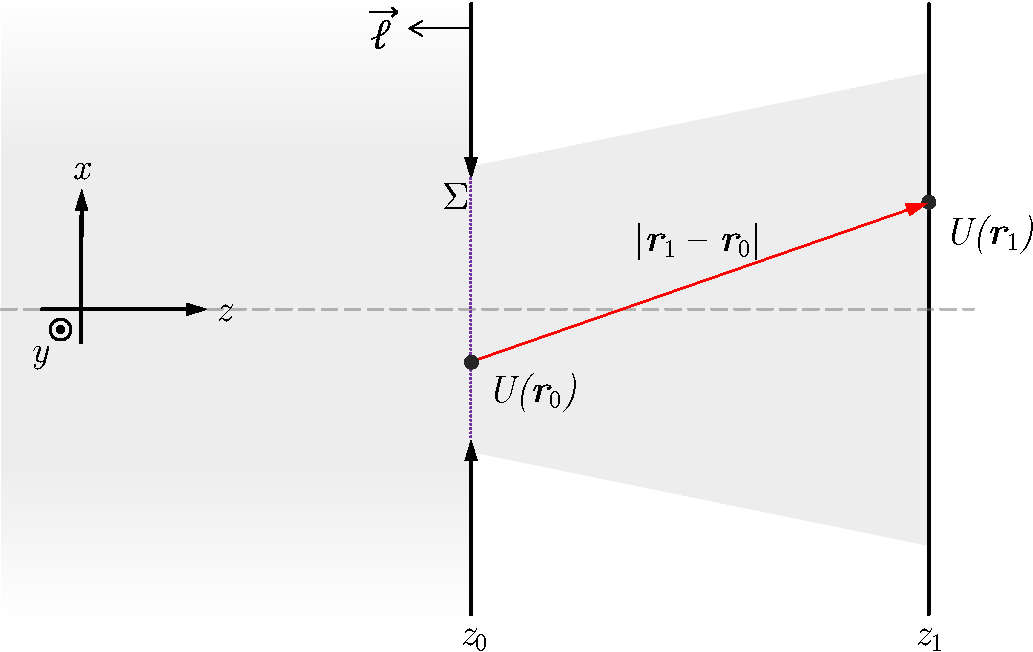
\includegraphics[width=.5\linewidth]{figures/ch02/diffraction_geometry.pdf}}
    \caption[Scalar diffraction problem geometry]{Scalar diffraction problem geometry. $\Sigma$ represents the input plane, where the electric field is completely defined, that is, $U(x_0, y_0, z_0)$ is known for all $(x_0, y_0, z_0)$, $\ell$ is a orthonormal vector to $\Sigma$. Scalar diffraction theory concerns the calculation of an electric field $U(x_1, y_1, z_1)$ in the output plane with the knowledge of it in the input plane.}
    \label{fig:diffraction}
\end{figure}

%-------------------------------------------------------------------------
%-------------------------------------------------------------------------
\subsubsection*{Fresnel diffraction}
%-------------------------------------------------------------------------
%-------------------------------------------------------------------------

Consider a Cartesian coordinate system where the $z-$axis is the optical axis (cf. Fig~\ref{fig:diffraction}), suppose a transverse component of a wave-field complying with Eq.~\ref{eq:Helmholtz} can be completely described at a position $z_0$, that is, $U(x,y,z_0)$ is known for all the $xy-$plane. The wave-field distribution in a parallel plane at a position $z_1$ of the optical axis can be calculated using the first Rayleigh-Sommerfeld diffraction equation [\cite[\textit{Eq.~3-42}]{Goodman2017}]:
\begin{equation}\label{eq:Huygens-Fresnel}
    U(\textbf{r}_1) = \frac{k}{i2\pi}\iint\limits_{\Sigma}{U(\textbf{r}_0)\frac{\exp{(ik\vert\textbf{r}_1 - \textbf{r}_0\vert)}}{\vert\textbf{r}_1 - \textbf{r}_0\vert}\cos{(\vec{\ell},\textbf{r}_1 - \textbf{r}_0)}~\mathrm{d}s},
\end{equation}
where $\textbf{r}_0=(x_0,y_0,z_0)$, $\textbf{r}_1=(x_1,y_1,z_1)$, $\vec{\ell}$ is a normal vector parallel to the optical axis and $\Sigma$ is the $xy-$plane in $z_0$ where the integration takes place - cf. Fig~\ref{fig:diffraction}. Eq.~\ref{eq:Huygens-Fresnel} assumes that $\vert\textbf{r}_1 - \textbf{r}_0\vert\gg\lambda$ and is often referred to as the Huygens-Fresnel principle\footnote{Eq.~\ref{eq:Huygens-Fresnel} expresses the wave-field evaluated in $\textbf{r}_1$, that is, $U(\textbf{r}_1)$ as a sum of spherical wave-fronts originating from a secondary sources modulated by $U(x_0,y_0,z_0)$ at each point $\textbf{r}_0$ within the aperture $\Sigma$.} [\cite[\textit{§3.7}]{Goodman2017}]. In the paraxial approximation $\cos{(\vec{\ell},\textbf{r}_1 - \textbf{r}_0)}\approx1$ and $\vert\textbf{r}_1 - \textbf{r}_0\vert=\sqrt{(x_1-x_0)^2+(y_1-y_0)^2+L^2}\approx L +[(x_1-x_0)^2+(y_1-y_0)^2]/2L$, where $L=z_1-z_0$ with $L\gg\vert x_1-x_0\vert$ and $L\gg\vert y_1-y_0\vert$. The latter is know as the Fresnel approximation. Eq.~\ref{eq:Huygens-Fresnel} can be simplified to:
\begin{equation}\label{eq:Fresnel}
    U(x_1,y_1,z_1)=\frac{k\exp{(ikL)}}{2\pi i L}\iint\limits_{-\infty}^{\hspace{8pt}\infty}{U(x_0,y_0,z_0)\exp{\Bigg\{\frac{ik}{2L}\big[(x_1-x_0)^2+(y_1-y_0)^2 \big]\Bigg\}}~\mathrm{d}x_0\mathrm{d}y_0},
\end{equation}
which is know as the Fresnel diffraction integral [\cite[\textit{§4.2}]{Goodman2017}]. The accuracy of Eq.~\ref{eq:Fresnel} is limited by the Taylor expansion of $\vert\textbf{r}_1 - \textbf{r}_0\vert=L\sqrt{1+\rho^2/L^2}$, where  $\rho = \sqrt{(x_1-x_0)^2+(y_1-y_0)^2}$, which is usually usually truncated on the linear term\footnote{The Taylor series expansion at $v=0$ is $\sqrt{1+v}=1+\frac{v}{2}-\frac{v^2}{8}+\frac{v^3}{16}+\mathcal{O}(v^4)$ and it converges for $\vert v\vert<1$.}, provided that the phase induced by the quadratic term of the expansion is much less than the Rayleigh's quarter-wave criterion, which limits the maximum phase error to $\pi/4$ radians [\cite[\textit{§9.3}]{born_wolf1999}]. Neglecting high-order terms in the approximation of the square-root in Eq.~\ref{eq:Fresnel} can be done if:
\begin{equation}\label{eq:accuracy_Fresnel}
    \sqrt[3]{\frac{\rho^4}{\lambda}}\ll z.
\end{equation}

%-------------------------------------------------------------------------
%-------------------------------------------------------------------------
\subsubsection*{Fraunhofer diffraction}
%-------------------------------------------------------------------------
%-------------------------------------------------------------------------

Still analysing Eq.~\ref{eq:Fresnel}, the quadratic term in the exponential part of the integrand can be expanded and rearranged: 
\begin{multline}\label{eq:Fresnel_2}
    U(x_1,y_1,z_1)=\frac{k\exp{(ikL)}}{2\pi i L}\exp{\Bigg[ \frac{ik}{2L}(x_1^2+y_1^2)\Bigg]}\cdot\\
    \cdot\iint\limits_{-\infty}^{\hspace{8pt}\infty}{U(x_0,y_0,z_0)\exp{\Bigg[\frac{ik}{2L}\big(x_0^2+y_0^2-2x_1x_0-2y_1y_0)\Bigg]}~\mathrm{d}x_0\mathrm{d}y_0}.
\end{multline}
Applying the Rayleigh's quarter-wave criterion to the $k(x_0^2+y_0^2)/2L$ term in Eq.~\ref{eq:Fresnel_2}:
\begin{equation}\label{eq:accuracy_Fraunhofer}
    4\frac{x_0^2 +y_0^2}{\lambda}\ll z,
\end{equation}
which allows to further simplify Eq.~\ref{eq:Fresnel} into:
\begin{multline}\label{eq:Fraunhofer}
    U(x_1,y_1,z_1)=\frac{k\exp{(ikL)}}{2\pi i L}\exp{\Bigg[ \frac{ik}{2L}(x_1^2+y_1^2)\Bigg]}\cdot\\
    \cdot\iint\limits_{-\infty}^{\hspace{8pt}\infty}{U(x_0,y_0,z_0)\exp{\Bigg[-\frac{ik}{L}\big(x_1x_0+y_1y_0)\Bigg]}~\mathrm{d}x_0\mathrm{d}y_0},
\end{multline}
Eq.~\ref{eq:Fraunhofer} is know as the Fraunhofer diffraction integral.

%-------------------------------------------------------------------------
%-------------------------------------------------------------------------
\subsubsection*{Numerical computation of the Fresnel and Fraunhofer diffraction}
%-------------------------------------------------------------------------
%-------------------------------------------------------------------------

The numerical calculation of the diffraction integrals is a vast subject and has been addressed by a plurality of authors [\cite{DArcio:94}], [\cite{Kelly2014}], [\cite[\textit{§5}]{Goodman2017}], [\cite{Buitrago-Duque:19}] and [\cite{Chubar2019}], among many others. This arises from the fact that unless the resulting field $U(x_1,y_1,z_1)$ has an analytical representation, numerically calculating the integrals in Eq.~\ref{eq:Fresnel} and Eq.~\ref{eq:Fraunhofer} will forcefully result in tackling issues like replicas and aliasing. This comes from the fact that the diffraction integrals are intimately connected with the Fourier analysis. 

Upon closer inspection, it is apparent that the Fresnel diffraction integral (Eq.~\ref{eq:Fresnel}) is a two-dimensional convolution type integral [\cite[\textit{§2.1}]{Goodman2017}]:
\begin{equation}\label{eq:conv}
    g(x,y) * h(x,y) = \iint\limits_{-\infty}^{\hspace{8pt}\infty}{g(u,v)h(x-u,y-u)~\mathrm{d}u\mathrm{d}v},
\end{equation}{}
which can be computed by invoking the convolution theorem:
\begin{equation}\label{eq:conv_theorem}
    g(x,y) * h(x,y) = \mathcal{F}^{-1}\big\{\mathcal{F}\{g(x,y)\}\cdot\mathcal{F}\{h(x,y)\}\big\},
\end{equation}{}
where $\mathcal{F}\{\bullet\}$ is the two-dimensional Fourier transform and $\mathcal{F}^{-1}\{\bullet\}$ denotes inverse Fourier transform:
\begin{subequations}\label{eq:Fourier}
    \begin{align}
        \mathcal{F}\{g\} &= \iint\limits_{-\infty}^{\hspace{8pt}\infty}{g(x,y)\exp{\big[-i2\pi(f_xx+f_yy)\big]}~\mathrm{d}x\mathrm{d}y}\\
        \mathcal{F}^{-1}\{G\} &=\iint\limits_{-\infty}^{\hspace{8pt}\infty}{G(f_x,f_y)\exp{\big[i2\pi(f_xx+f_yy)\big]}~\mathrm{d}f_x\mathrm{d}f_y}.
    \end{align}
\end{subequations}{}
It is common to represent the Fourier analysis and syntheses as $\mathcal{F}\{g(x,y)\}\equiv G(f_x,f_y)$ and $\mathcal{F}^{-1}\{G(f_x,f_y)\}\equiv g(x,y)$, where $(f_x,f_y)$ are generally referred to as frequencies. The Fresnel diffraction integral in Eq.~\ref{eq:Fresnel} can be rewritten as a convolution (Eq.~\ref{eq:conv_theorem}) where the kernel, that is $\mathcal{F}\{h(x,y)\}$, has analytical solution:
\begin{equation}\label{eq:kernel}
     \frac{k}{2\pi i L}\mathcal{F}\{h(x,y)\} = \frac{k}{2\pi i L}\mathcal{F}\Bigg\{
    \exp\bigg[\frac{ik}{2L}\big(x^2+y^2 \big)\bigg]\Bigg\} = \exp{\bigg[-\frac{i2L\pi^2}{k} \big(f_x^2+f_y^2 \big)\bigg]},
\end{equation}
%with $f_x=x/(\lambda L)$ and $f_y=y/(\lambda L)$.
This formulation allows to calculate the Fresnel diffraction integral (Eq.~\ref{eq:Fresnel}) by means of the convolution theorem (Eq.~\ref{eq:conv_theorem}) by applying a Fourier transform to the input field, multiplying it by an analytical kernel and applying an inverse Fourier transform to the result. It is also evident that the Fraunhofer diffraction integral (Eq.~\ref{eq:Fraunhofer}) is a Fourier type integral, differing from Eq.~\ref{eq:Fourier}a by a multiplicative factor outside the integrand. 

\begin{figure}[t]
    \centering
    {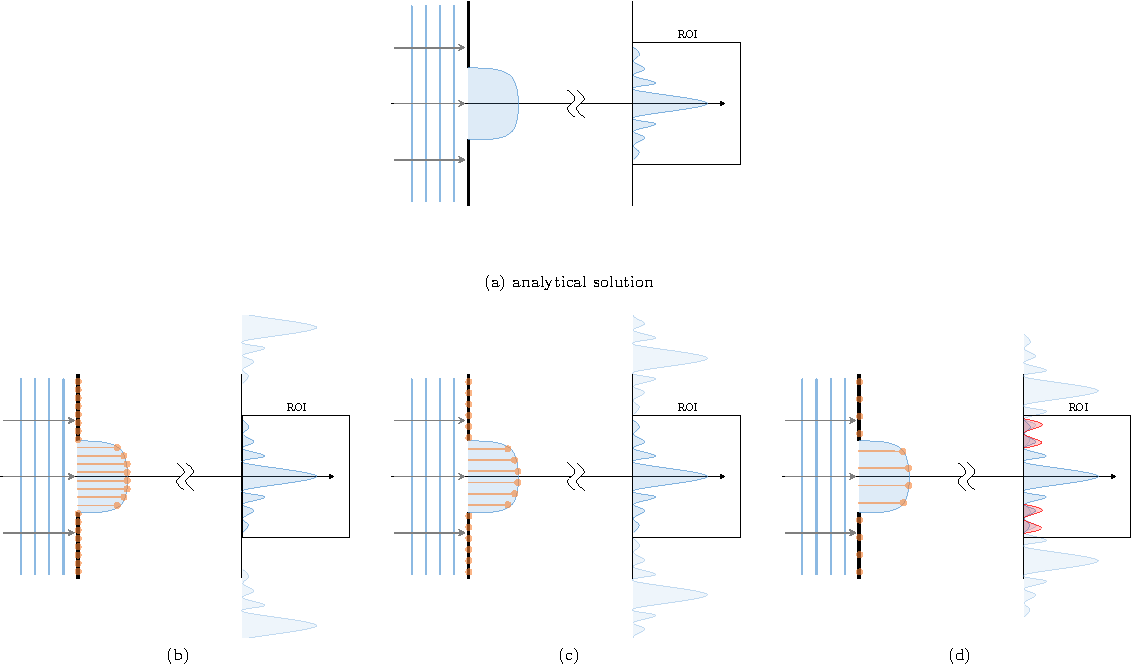
\includegraphics[width=1\linewidth]{figures/ch02/sampling_aliasing.pdf}}
    \caption[Replicas and aliasing]{Replicas and aliasing from numeric calculations of the diffraction integrals. (a) analytical solution of the integrals have no signal replicas. Sampling the input plane signal will introduce replicas in the output plane [\cite{Kelly2014}]. (b) appropriate sampling - cf. Eq.~5 in [\cite{Chubar2019}] - makes the unavoidable replicas further enough that cross-talk between them is negligible within the region of interest (ROI). (c) coarser sampling brings replicas closer up to a point that (d) replicas are so close that aliasing is eminent (red signal).}
    \label{fig:sampling}
\end{figure}

It should be clear, then, that the paraxial diffraction equations are intertwined with Fourier analysis. Numerically computation of the Fresnel or Fraunhofer diffraction implies \textit{a}-) sampling the input plane $U(x_0,y_0,z_0)$ and \textit{b}-) limiting its extent by either defining an aperture of finite extent or simply by cropping (truncating) the input field. It follows from sampling theory and the discrete Fourier transform (DFT) [\cite[\textit{§10}~\&~\textit{§11}]{Bracewell2000}] that sampling the input field causes replicas of the main signal to appear (cf. Fig.~\ref{fig:sampling}). Generally, the finer the sampling in the input plane, the further apart the replicas are. Consequently, the coarser the mesh gets, the closer they get up to a point that the replicas are close enough to each other that they start cross-talking. The interaction between the main signal and its replicas is called aliasing. Due to the finite extent of the input plane (either by limiting the signal with an aperture or by simply truncating it), it is inevitable that power from neighbouring replicas leak into each other. Sampling should be high enough as to make this inevitable cross-talk negligible [\cite{Kelly2014}]. On the other hand, a very large sampling leads to very inefficient calculations largely because of the size of the input and output planes - cf. considerations in [\cite[\textit{§5}]{Goodman2015}]. Efforts towards a memory and CPU efficient computation of the Fresnel free-space propagator in Fourier optics have been reported in [\cite{Chubar2019}].

%-------------------------------------------------------------------------
%-------------------------------------------------------------------------
\subsection{Transmission elements}\label{sec:thin_element}
%-------------------------------------------------------------------------
%-------------------------------------------------------------------------

The propagation of X-rays in the presence of matter can also be modelled with the Maxwell equations (Eqs.~\ref{eq:Maxwell}). It is possible to derive a Helmholtz equation in the presence of scatterers with a similar treatment given in the previous section, albeit considerably more algebraic - a detailed account of the derivation is given by [\cite[\textit{§2.1}]{Paganin2006}]. Restricting the analysis to linear isotropic non-magnetic materials where both the electric permittivity and magnetic permeability are independent of time (static medium) and considering again that the waves exist in a uncharged and non-conducting material,  that is, $\rho=0$ and $\textbf{J}=\textbf{0}$:
\begin{subequations}\label{eq:dAllembert_inho}
    \begin{align}
        \Bigg[\varepsilon(x,y,z)\mu_0\frac{\partial^2}{\partial t^2} - \nabla^2 \Bigg]\textbf{E}(x,y,z,t) &= \textbf{0}, \\
        \Bigg[\varepsilon(x,y,z)\mu_0\frac{\partial^2}{\partial t^2} - \nabla^2 \Bigg]\textbf{B}(x,y,z,t) &=\textbf{0}.
    \end{align}
\end{subequations}{}
considering that the scatterers are sufficiently slowly varying when compared to the radiation wavelength - cf. Eqs.~2.18-2.21 in [\cite{Paganin2006}]. Eqs.~\ref{eq:dAllembert_inho} resemble the vectorial wave-equations \ref{eq:Evectorial_waveeq} and \ref{eq:Bvectorial_waveeq}. This enables to give the same scalar treatment used for deriving the Helmholtz equation in free-space, that is, to propose a scalar field $u(x,y,z,t)$ such as:
\begin{equation}\label{eq:Scalar_WE_inho}
    \Bigg[\varepsilon(x,y,z)\mu_0\frac{\partial^2}{\partial t^2} - \nabla^2\Bigg]u=0,
\end{equation}
and spectrally decompose $u$ in its monochromatic Fourier components $U(x,y,z)\exp{(-i\omega t)}$ (cf. Eq.~\ref{eq:spectral_decomposition}):
\begin{equation*}
    u(x,y,z,t)=\frac{1}{\sqrt{2\pi}}\int\limits_{-\infty}^\infty{U(x,y,z)\exp{(-i\omega t)}~\mathrm{d}\omega}
\end{equation*}
This Fourier integral can be plugged into Eq.~\ref{eq:Scalar_WE_inho}, which leads to the Helmholtz equation in the presence of scatterers\footnote{cf. [\cite[\textit{Eq.~2.28}]{Paganin2006}].}:
\begin{equation}\label{eq:Helmholtz_inho}
    \big[\nabla^2 + k^2n^2(x,y,z)\big]U(x,y,z) = 0,
\end{equation}{}
where $n$ is the wavelength-dependent refractive index such that $n(x,y,z)^2\equiv\varepsilon(x,y,z)/\varepsilon_0$. This version of the Helmholtz equation for a inhomogeneous medium can rarely be solved exactly and approximations are necessary to handle it [\cite[\textit{§2.1}]{Paganin2006}]. The same argument used to derive the paraxial Helmholtz equation (Eq.~\ref{eq:Helmholtz_paraxial}) can be applied here. Assuming a plane wave (Eq.~\ref{eq:planewave}) modulated by a complex envelope $A(\textbf{r})$ slowly varying along a distance $\lambda$ and plugging it into Eq.~\ref{eq:Helmholtz_inho}, one arrives to:
\begin{equation}\label{eq:Helmholtz_inho_paraxial}
    \Bigg\{2ik\frac{\partial}{\partial z}-\nabla^2_T+k^2\big[n^2(x,y,z)-1\big]\Bigg\}A=0.
\end{equation}{}
which is known as the paraxial Helmholtz equation in matter. Eq.~\ref{eq:Helmholtz_inho_paraxial} is compatible to the treatment used for propagating the wave-fields in free-space - cf. [\cite[\textit{Eq.~2.33}]{Paganin2006}]. Notice that Eq.~\ref{eq:Helmholtz_inho_paraxial} reduces to Eq.~\ref{eq:Helmholtz_paraxial} for $n=1$.

%-------------------------------------------------------------------------
%-------------------------------------------------------------------------
\subsubsection*{The projection approximation}
%-------------------------------------------------------------------------
%-------------------------------------------------------------------------

\begin{figure}[t]
    \centering
    {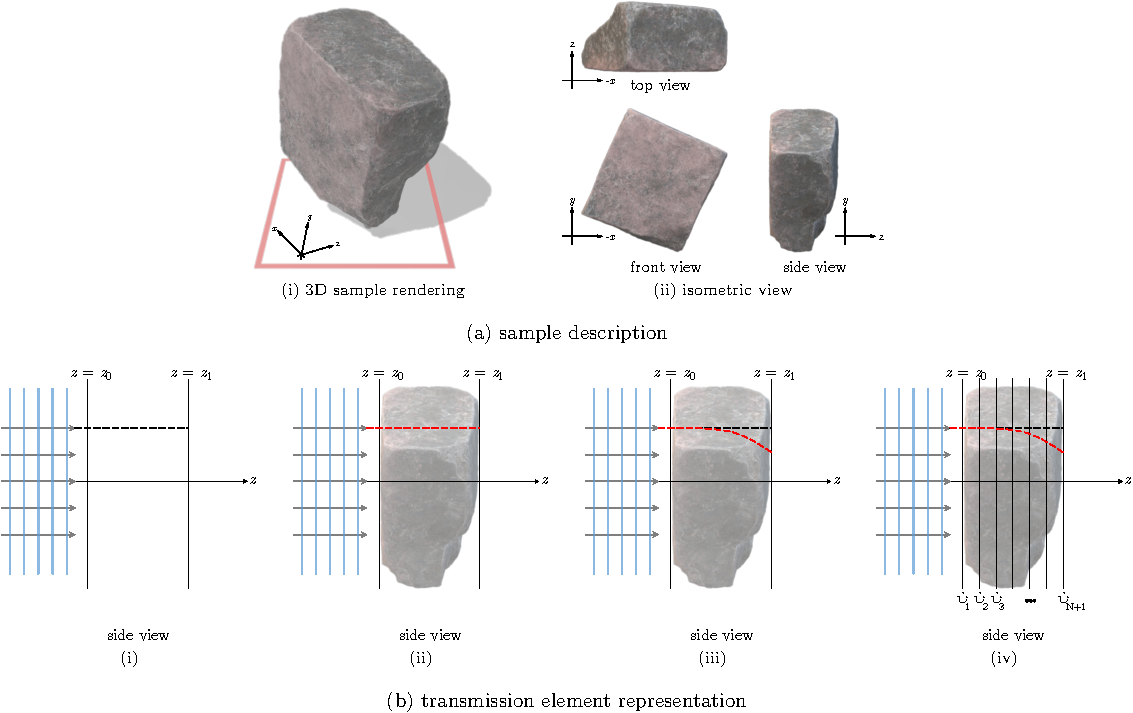
\includegraphics[width=1.0\linewidth]{figures/ch02/projection_approx.pdf}}
    \caption[Transmission elements]{(a) arbitrary-shaped scattering volume in free-space. (b) transmission element representation of said scatterer. The 3D model was taken from the \textit{3D shapes} library in the Paint 3D software from the Microsoft Corporation.}
    \label{fig:projection}
\end{figure}
Consider an arbitrary-shaped scattering volume as shown in Fig.~\ref{fig:projection}(a). Suppose that such scatterer is completely confined within a region $z_0\leq z\leq z_1$ and outside that there is vacuum. Let this sample be illuminated by a plane-wave moving along the positive direction of the optical axis ($z-$axis). In the absence of the scatterer, the gradient between the $z=z_0$ and $z=z_1$ planes is very well defined and parallel to the optical axis, as shown in Fig.~\ref{fig:projection}(b-$\mathrm{i}$). It follows from [\cite[\textit{§2.2}]{Paganin2006}] that if the scatterer is sufficiently weak as to minimally disturb the path that the wave-field would have taken in its absence, cf. Fig.~\ref{fig:projection}(b-$\mathrm{ii}$), the transmission of a wave-field through this sample is given by:
\begin{equation}\label{eq:transmission_n}
    U(x,y,z_1)\approx\exp\Bigg\{-\frac{ik}{2}\int\limits_{z=z_0}^{z=z_1}{\big[1-n^2(x,y,z)\big]~\mathrm{d}z}\Bigg\}U(x,y,z_0).
\end{equation}{}
Eq.~\ref{eq:transmission_n} shows that the effect of a weak scatterer can be accounted by a multiplicative complex transmission element represented by the complex exponential. In the X-ray regime the index of refraction is typically very close to the unity and often expressed as $n=1-\delta+i\cdot\beta$ [\cite[\textit{§1.6}]{Als-Nielsen2011}], which allows for the approximation $1-n(x,y,z)^2\approx2\big[\delta(x,y,z)+i\cdot\beta(x,y,z)\big]$ that can be substituted in Eq.~\ref{eq:transmission_n}. The $z-$dependence of $\delta$ and $\beta$ is abandoned in the projection approximation, hence the complex transmission element in Eq.~\ref{eq:transmission_n} can be reduced to:
\begin{align}\label{eq:transmission}
\mathrm{T}(x,y,z) &=\exp\Bigg\{-ik\int\limits_{z=z_0}^{z=z_1}{\big[\delta(x,y)+i\cdot\beta(x,y)\big]~\mathrm{d}z}\Bigg\}\nonumber\\
         &=\exp\Bigg\{-ik\big[\delta(x,y)+i\cdot\beta(x,y)\big]\Delta_z(x,y)\Bigg\},\nonumber\\
\mathrm{T}\big[\Delta_z(x,y)] &=\sqrt{\mathrm{T}_\text{BL}(x,y)}\exp{\big[i\phi(x,y)\big]}.
\end{align}{}
and:
\begin{subequations}
\begin{align}   
    \mathrm{T}_{\text{BL}}(x,y)&=\exp{\big[-2k\beta(x,y)\Delta_z(x,y)\big]}\label{eq:aux_funcs_transa}  \\
    &=\exp{\big[-\mu(x,y)\Delta_z(x,y)\big]},\nonumber\\
    \phi(x,y)&=-k\delta(x,y)\Delta_z(x,y).\label{eq:aux_funcs_transb}
\end{align}
\end{subequations}
$\Delta_z$ is the projected thickness along the $z-$axis and it depends on the transverse coordinates $(x,y)$, which can be dropped out for a more concise representation.

Because of the multiplicative nature of the transmission element, Eq.~\ref{eq:transmission} can be put in operator\footnote{Using the operator formulation was inspired by discussions with David Paganin (Monash University, Australia) and Vincent Favre-Nicolin (ESRF, France).} form:
\begin{equation}\label{eq:transmission_operator}
    \mathrm{T}(\Delta_z)~\bullet =\sqrt{\mathrm{T}_\text{BL}(\Delta_z)}\exp{[i\phi(\Delta_z)]}~\bullet.
\end{equation}
Eq.~\ref{eq:aux_funcs_transa} shows the absorption experienced by the wave-field when passing through matter (Beer-Lambert law) and Eq.~\ref{eq:aux_funcs_transb} shows the phase-shift experienced by the wave-field. The coefficient $\mu$ multiplying $\Delta_z$ in $\mathrm{T}_{\text{BL}}$ (Eq.~\ref{eq:aux_funcs_transa}) is know as linear attenuation coefficient $\mu$ [\cite[\textit{§1.6}]{Als-Nielsen2011}]. 

%-------------------------------------------------------------------------
%-------------------------------------------------------------------------
\subsubsection*{The multi-slice approximation}
%-------------------------------------------------------------------------
%-------------------------------------------------------------------------

For the cases where the projection approximation may not be adequate to correctly represent the scattering volume in question, multi-slicing techniques (MS) can be used for describing the wave-field propagation inside an arbitrary-shaped scattering volume - cf. discussion in [\cite[\textit{§2.7}]{Paganin2006}], [\cite{Li2017}] and [\cite{Munro2019}].

Consider the scatterer depicted in Fig.~\ref{fig:projection}(a). If its presence considerably disturbs the path that the wave-field would have taken in its absence, cf. Fig.~\ref{fig:projection}(b-$\mathrm{iii}$), it is possible to section the sample into a number $N$ of parallel slabs until the projection approximation is valid between two adjacent slices - Fig.~\ref{fig:projection}(b-$\mathrm{iv}$). The projected thickness $\Delta_z$ to be used in Eq.~\ref{eq:transmission} is the one in the between slices, which are $\Delta_S=(z_1 - z_0)/N$ apart from each other. Each slice represented as a thin element in projection approximation is separated by vacuum. The propagation of a wave-field propagation through this sample is done step-wise, where each step is composed of a multiplication by a complex transmission element in projection approximation (cf. Eq.~\ref{eq:transmission}) and a Fresnel free-space propagation (Eq.~\ref{eq:Fresnel}) over a distance $\Delta_S$. The output field from this operation is again multiplied by complex transmission element in projection approximation followed by a free-space propagation from the plane $\psi_j$ to the  $\psi_{j+1}$ - refer to Fig.~\ref{fig:projection}(b-$\mathrm{iv}$). This operation is done recursively $N$ times until the wave-field emerges from the sample. The multi-slicing transmission operator can be written in operator form as:
\begin{align}\label{eq:MS}
    \mathrm{T}_\text{MS}=\prod\limits_{j=1}^{N}\mathcal{D}(\Delta_S)\big[\mathrm{T}_j(\Delta_z)~\bullet\big]
\end{align}{}
where $\prod$ indicates concatenation of operators to be performed from right to left, $\mathcal{D}(\Delta_S)$ is the operator formulation of the Fresnel free-space propagation over a distance $\Delta_S$:
\begin{equation}\label{eq:Fresnel_operator}
    \mathcal{D}(\Delta_S)~\bullet=\frac{k\exp{(ik\Delta_S)}}{2\pi i \Delta_S}\iint\limits_{-\infty}^{\hspace{8pt}\infty}{\bullet~\exp{\Bigg\{\frac{ik}{2\Delta_S}\big[(x_1-x)^2+(y_1-y)^2 \big]\Bigg\}}~\mathrm{d}x\mathrm{d}y},
\end{equation}
and $\mathrm{T}_j(\Delta_z)$ is the $j-$th complex transmission element operator in projection approximation associated with the $j-$th slice given by Eq.~\ref{eq:transmission_operator}.

%-------------------------------------------------------------------------
%-------------------------------------------------------------------------
\subsubsection*{-- On the validity of the Fresnel approximation for short propagation distances\footnote{The author acknowledges the fruitful discussions with David Paganin (Monash University, Australia), Peter Munro (University College London, England), Oleg Chubar (Brookhaven National Lab., USA) and Chris Jacobsen (Northwestern University/Argonne National Lab., USA) when investigating the application of the Fresnel approximation for short propagation distances.}}
%-------------------------------------------------------------------------
%-------------------------------------------------------------------------

A case of particular importance for X-ray optical design is the is application of the Fresnel propagators in real or reciprocal space to very short propagation distances (from millimetres to hundreds of micrometres) at hard X-ray energies (wavelength of the order of the \r{A}ngstrom) with physical apertures of the order of the millimetre. For situations of practical interest such as the one just described, Eq.~\ref{eq:accuracy_Fresnel} is generally very restrictive. This section presents conditions under which said constraint can be relaxed and even overlooked. 

Consider an X-ray wavefield with wavelength $\lambda=1~\AA$ fully illuminating an aperture $A=500$~\textmu m situated at $z=z_0$ along the optical axis as shown in Fig.~\ref{fig:diffraction}. The X-rays passing through such an aperture will illuminate an identical aperture $A$ at a distance $z_1-z_0=L$. Suppose one wants to place the second aperture a distance $L$ such as it is possible to calculate the field distribution in $z_1$ using the Fresnel diffraction integral in Eq.~\ref{eq:Fresnel}. Using Eq.~\ref{eq:accuracy_Fresnel} with the extreme points\footnote{For simplicity, the 1D case is analysed, but the conclusions are easily translated to a 2D system if $U(x,y)=U(x)U(y)$.} given by $(x_0=-A/2, y_0=0)$ and $(x_1=A/2, y_1=0)$, one concludes that $ L\gg86~$mm. However, if one wants to place the second aperture at a distance of $L=1$~mm and still be able to safely apply Eq.~\ref{eq:Fresnel} to calculate the field distribution in $z_0$, the apertures should be reduced to $A\ll18~$\textmu m according to Eq.~\ref{eq:accuracy_Fresnel}. The situation just described is at odds with the employment of the Fresnel propagator for very short propagation distances at hard X-ray energies with physical apertures of the order of the millimetre. Yet, with the exception of [\cite{Ali2020}], that explicitly uses the Huygens-Fresnel principle [\cite[\textit{\S3.7}]{Goodman2017}] in its reciprocal form for the wavefield propagation\footnote{cf. Eq.~22 or procedure \textit{PropShort} in Algorithm 1 from [\cite{Ali2020}].}, authors make extensive use of the Fresnel propagator for multi-slicing applications under said conflicting conditions [\cite{Li2017, Munro2019, Celestre2020}]. Possibly one of the few explicit mentions of the propagation distance relation to the transverse plane size applied to multi-slicing techniques is given by Eq.~15 in [\cite{Ishizuka1977}]. It turns out that, indeed, Eq.~\ref{eq:accuracy_Fresnel} when applied to a collimated beam (either a plane-wave or a slowly diverging/converging wave) is too restrictive and can be overlook when applied to MS modelling of weak scatteres.

In [\cite{Southwell1981}] the Fresnel diffraction integral (Eq.~\ref{eq:Fresnel}) is directly compared with the Huygens-Fresnel integral (Eq.~\ref{eq:Huygens-Fresnel}) in terms of amplitude and phase, it was shown that the Fresnel approximation has good accuracy: within 2\% in amplitude and 0.02~rad in phase, when compared to the Huygens-Fresnel integral. The findings hold even for very high Fresnel numbers\footnote{The Fresnel number is defined as $N_F=a^2/\lambda L$, where $a$ is the half aperture, $\lambda$ is the wavelength and $L$ is the propagation distance. A high Fresnel number indicates the region know as near-field, while the far-field region is know for its low Fresnel numbers. In [\cite{Southwell1981}], it is reported that even for $L<a$ good agreement between the Fresnel approximation and the Huygens-Fresnel integral is found for a point within the projected aperture.} along the optical axis within the projected aperture, that is, $\forall~(x,y) \in A$ - [cf. Figs.~1--4 ibid.]. However, for points outside that region ($\forall~(x,y) \notin A$) at very high Fresnel numbers (shadow region), the approximation breaks down: although the amplitude calculation retains good agreement, the phase errors become unacceptably high [cf. Fig.~10 ibid.]. 

\begin{figure}[t]
    \centering
    {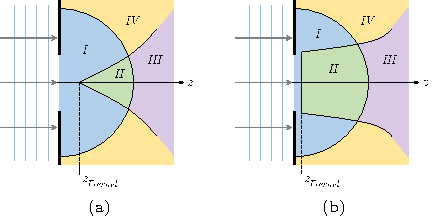
\includegraphics[width=0.6\linewidth]{figures/ch02/Fresnel.pdf}}
    \caption[The validity of the Fresnel approximation]{The Fresnel and Fraunhofer approximations region of validity according to the (a) Eqs.~\ref{eq:accuracy_Fresnel} and \ref{eq:accuracy_Fraunhofer}. For a gently divergent, convergent or plane wavefield the constraints can be relaxed, increasing the region o applicability of said approximations. Region \textit{I} represents the shadow zone, where neither approximations are valid. Region \textit{II} is where only the Fresnel approximation is valid. In region \textit{III}, both approximations coexist, the Fraunhofer being advantageous computationally. Region \textit{IV} illustrates an area where only the Fraunhofer approximation is valid - this counter-intuitive result is discussed in [\cite{Rees87}], but is out of the scope here. The boundaries between regions \textit{I} and \textit{II} have been exaggerated for clarity. This figure is adapted from Fig.~4 and Fig.~5 in [\cite{Rees87}].}
    \label{fig:validity_fresnel}
\end{figure}

Another study that confirms the validity of the Fresnel approximation for a collimated beam being propagated over a very short distance in presented by [\cite{Rees87}]. This work not only confirms the numerical findings in [\cite{Southwell1981}], but also provides physical explanations, some analytical formulations and derives quantitatively the shape of the region where the Fresnel approximation is valid. By applying directly Eq.~\ref{eq:accuracy_Fresnel} and  Eq.~\ref{eq:accuracy_Fraunhofer}, one obtains the the regions of validity for both Fresnel and Fraunhofer integrals as in Fig.~\ref{fig:validity_fresnel}(a), in which case, $z_{Fresnel}$ is given by Eq.~\ref{eq:accuracy_Fresnel} - cf. Eq.~7 in [\cite{Rees87}]. The relaxing of such constrains is done by invoking the concept of Fresnel zones\footnote{cf. [\cite[\textit{§10.3.1}]{Hetch2017}]} and how much contribution it has to the total amplitude and phase of the propagated beam. Considering that the first zone is unobstructed by the aperture $A$, which is the case for all points not within the shadow region, the distance where the Fresnel diffraction integral starts to be accurate can be as low as $z_{Fresnel}=2\lambda$ - cf. Eq.~9 in [\cite{Rees87}]. This is relaxed regime is represented in Fig.~\ref{fig:validity_fresnel}(b).

Based on the results from [\cite{Southwell1981}] and [\cite{Rees87}], it is possible to affirm that provided the object is illuminated with a plane wave and the output field is calculated in the vicinity of the projected aperture, the application of the Fresnel diffraction integral to very short propagation distances for hard X-ray optics modelling with MS techniques is not limited to the constraints imposed by Eq.~\ref{eq:accuracy_Fresnel}. Cases of interest often have non-plane-wave illumination and require special handling to ensure MS with the Fresnel diffraction integral yields accurate results. Approaches that rely on spherical-to-plane-wave conversion are often employed to avoid such accuracy issues: the angular spectrum of plane waves decomposition [\cite[\textit{\S1.3}]{Paganin2006}]\footnote{Also in [\cite[\textit{\S3.10}~\&~\textit{\S4.2.4}]{Goodman2017}].}, the Fresnel-scaling theorem [\cite[\textit{\S A}]{Paganin2006}], the divergent-beam-to-plane-wave transformation from [\cite{Munro2019}] and the analytical treatment of the quadratic phase term [\cite{Chubar2019}], which is of particular interest within the context of this work, as it is the chosen method for the free-space wavefront propagation simulations presented here. 

%-------------------------------------------------------------------------
%-------------------------------------------------------------------------
\subsubsection*{\normalsize -- Real and reciprocal space Fresnel propagators at short propagation distances }
%-------------------------------------------------------------------------
%-------------------------------------------------------------------------

Because of the equivalency of the Fresnel diffraction integral (Eq.~\ref{eq:Fresnel}) and the convolution integral (Eq.~\ref{eq:conv}), one can define the kernel of the Fresnel transform in real-space as:
\begin{align}\label{eq:kernel_real}
    h(x,y)=\exp\bigg[\frac{i\pi}{\lambda L}\big(x^2+y^2 \big)\bigg],
\end{align}{}
while the kernel of the Fresnel transform in reciprocal-space is given by:
\begin{align}\label{eq:kernel_reciprocal}
    H(f_x,f_y)=\exp{\bigg[-i\pi\lambda L\big(f_x^2+f_y^2 \big)\bigg]}.
\end{align}{}
The Eqs.~\ref{eq:kernel_real} and \ref{eq:kernel_reciprocal} are related by: $H(f_x,f_y)=i/(\lambda L)\cdot \mathcal{F}\{ h(x,y)\}$ (cf. Eq.~\ref{eq:kernel}). When propagating a wave-field over a very small distance $L$ with the Fresnel diffraction integral, the argument of the exponential function in transformation kernel in real-space becomes very large and the kernel becomes less well-behaved due to fast oscillations, consequently small propagation distances are better represented in the reciprocal space. This hints to the fact that when numerically evaluating the Fresnel transform for short propagation distances, methods using the reciprocal-space are more advantageous than in real-space and constrains like the Eq.~\ref{eq:accuracy_Fresnel} can be overlooked provided the non-paraxial components of the Fourier spectrum of the input wavefield is negligible.

% The Eqs.~\ref{eq:kernel_real} and \ref{eq:kernel_reciprocal} are related by: $H(f_x,f_y)=i/(\lambda L)\cdot \mathcal{F}\{ h(x,y)\}$ (cf. Eq.~\ref{eq:kernel}). When propagating a wave-field over a very small distance $L$ with the Fresnel diffraction integral, the argument of the exponential function in transformation kernel in real-space becomes very large and the kernel becomes less well-behaved as shown in  Fig.~\ref{fig:real_reciprocal}(a)-(b), consequently small propagation distances are better represented in the reciprocal space - cf. Fig.~\ref{fig:real_reciprocal}(c)-(d). This hints to the fact that when numerically evaluating the Fresnel transform for short propagation distances, methods using the reciprocal-space are more advantageous than in real-space and constrains like the Eq.~\ref{eq:accuracy_Fresnel} can be overlooked provided the non-paraxial components of the Fourier spectrum of the input wavefield is negligible.

% \begin{figure}[t]
%     \centering
%     {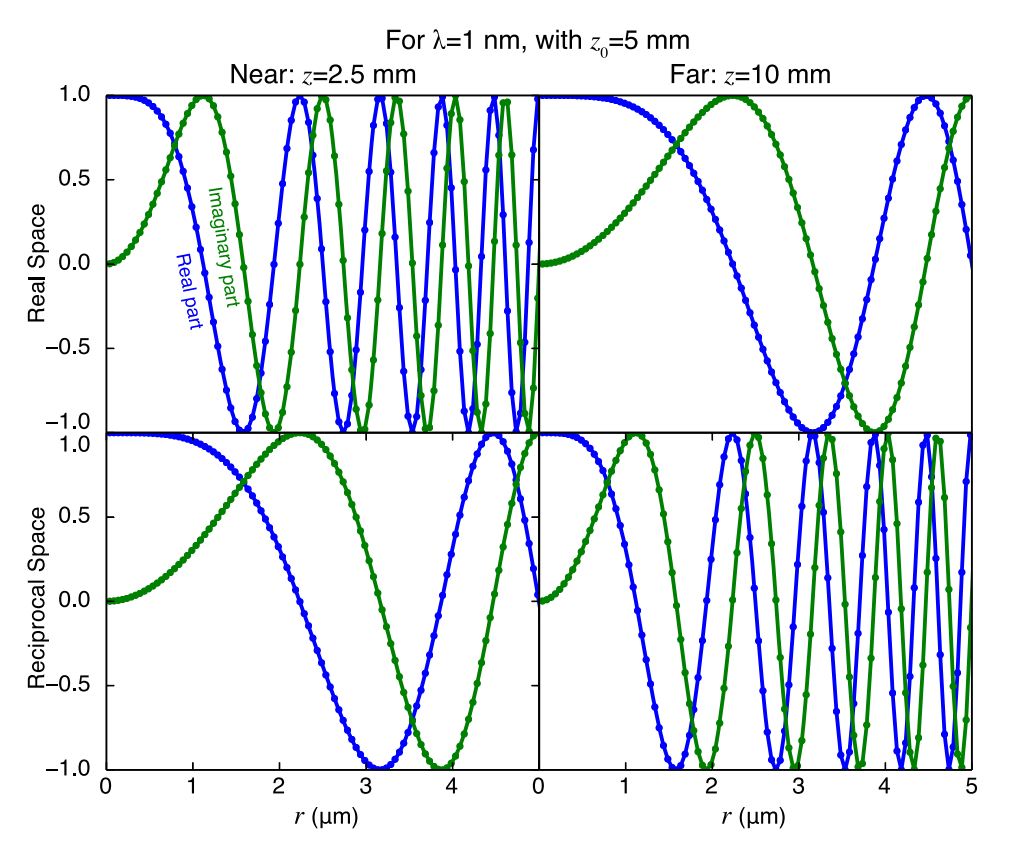
\includegraphics[width=0.5\linewidth]{figures/ch02/real_reciprocal.png}}
%     \caption[Frensel transformation kernel in real and reciprocal space]{Real-space kernel of the Fresnel transformation for (a) a short propagation distance and for a (b) longer propagation distance. The reciprocal-space propagator kernel is shown in (c) for a small propagation distance and in (d) for a longer distance. Adapted from Fig.~1 in [\cite{Li2015}].}
%     \label{fig:real_reciprocal}
% \end{figure}
%-------------------------------------------------------------------------
%-------------------------------------------------------------------------
\subsubsection*{\normalsize -- The analytical treatment of the of the quadratic radiation phase term\footnote{The analytical treatment of the of the quadratic radiation phase terms was introduced in 2007 for the SRW code [\cite{Chubar2008}] (cf. §\ref{sec:wave_propag} in §\ref{sec:optical_simulations}~-~\textit{\nameref{sec:optical_simulations}}). A more detailed description of the memory and CPU efficient computation of the Fresnel free-space propagator in Fourier optics simulations is given by [\cite{Chubar2019}], from which this section is partially based on.}}
%-------------------------------------------------------------------------
%-------------------------------------------------------------------------

Consider a non-collimated wave-field $U(x_0,y_0,z_0)$ in free-space (eg. Eq.~\ref{eq:spherical}). The phase term of such wave has quadratic terms with radii of curvature in the horizontal and vertical planes $R_x$ and $R_y$ and the transverse coordinates of the centre point $(x_\text{c},y_\text{c})$. It is possible to rewrite $U(x_0,y_0,z_0)$ as:
\begin{align}\label{eq:Semi_a}
    U(x_0,y_0,z_0) = F(x_0,y_0,z_0)\exp{\Bigg\{\frac{ik}{2}\Bigg[\frac{(x_0-x_c)^2}{R_y}+\frac{(y_0-y_c)^2}{R_y} \Bigg]\Bigg\}},
\end{align}{}
where $F(x_0,y_0,z_0)$ is the residual wavefront after the quadratic phase term is factorised. This residual wave-field satisfies the necessary conditions for the compliance with the Fresnel propagation of collimated beams through very short propagation distances as required by [\cite{Southwell1981}] and [\cite{Rees87}]. Substituting Eq.~\ref{eq:Semi_a} in the Fresnel diffraction integral (Eq.~\ref{eq:Fresnel}):
\begin{multline}\label{eq:Semi_b}
    U(x_1,y_1,z_1)=\frac{k\exp{(ikL)}}{2\pi i L}\iint\limits_{-\infty}^{\hspace{8pt}\infty}{F(x_0,y_0,z_0)}\cdot\\ \cdot{\exp{\Bigg\{\frac{ik}{2}\Bigg[\frac{(x_1-x_0)^2+(y_1-y_0)^2}{L}+\frac{(x_0-x_c)^2}{R_y}+\frac{(y_0-y_c)^2}{R_y} \Bigg]\Bigg\}}~\mathrm{d}x_0\mathrm{d}y_0},
\end{multline}
which can be conveniently expressed as: 
\begin{align}\label{eq:Semi_c1}
    U(x_1,y_1,z_1) = F(x_1,y_1,z_1)\exp{\Bigg\{\frac{ik}{2}\Bigg[\frac{(x_1-x_c)^2}{R_y+L}+\frac{(y_1-y_c)^2}{R_y+L} \Bigg]\Bigg\}},
\end{align}{}
with:
\begin{multline}\label{eq:Semi_c2}
    F(x_1,y_1,z_1)=\frac{k\exp{(ikL)}}{2\pi i L}\iint\limits_{-\infty}^{\hspace{8pt}\infty}{F(x_0,y_0,z_0)}\cdot\\ \cdot{\exp{\Bigg\{\frac{ik}{2L}\Bigg[\frac{R_x + L}{R_x}\Bigg(\frac{R_xx_1+Lx_c}{R_x+L} - x_0\Bigg)^2+\frac{R_y + L}{R_y}\Bigg(\frac{R_yy_1+Ly_c}{R_y+L} - y_0\Bigg)^2\Bigg]\Bigg\}}~\mathrm{d}x_0\mathrm{d}y_0}.
\end{multline}
It is evident that much like Eq.~\ref{eq:Fresnel}, Eq.~\ref{eq:Semi_c2} is a convolution-type integral with analytical Fourier transform of the convolution kernel, hence the discussion presented in \textit{Numerical computation of the Fresnel and Fraunhofer diffraction} in \S\ref{sec:free-space}~-~\textit{\nameref{sec:free-space}} is still applicable and the advantages of the wave propagation at very short distances in reciprocal space are maintained. The analytical treatment of the of the quadratic radiation phase term reduces significantly the required transverse sampling of the wave-field without compromising the compromising the accuracy of calculation, as the oscillations of the residual electric field are less rapid and require less dense sampling. Another advantage of such rewriting of the Fresnel diffraction integral is that the convolution shown in Eq.~\ref{eq:Semi_c2} takes place with respect to the scaled transverse coordinates $x_1\cdot R_x/(R_x+L)$ and $y_1\cdot R_y/(R_y+L)$. When using the convolution-theorem formulation of free-space propagation (cf. Eqs.~\ref{eq:conv} and \ref{eq:conv_theorem}), the scaled coordinates re-scale without any additional re-sampling nor interpolation the output plane by $\Delta x_1 = \Delta x_0 \cdot (R_x+L)/R_x$ and  $\Delta y_1 = \Delta y_0 \cdot (R_y+L)/R_y$, where $\Delta x_0$ and $\Delta y_0$ are the input plane dimensions. The formulation shown in Eqs.~\ref{eq:Semi_c1} and \ref{eq:Semi_c2} has singularities at $R_x+L = 0$ and $R_y+L = 0$, which happens when calculating the propagation of a wavefront after a focusing element at the image plane. The singularities can be dealt with by simply applying a $R_x'\neq0$ and $R_y'\neq0$ such as they are near $R_x$ and $R_y$, but avoid the singularity. Using  $R_x'\neq0$ and $R_y'\neq0$ still reduces the required transverse sampling and re-scales the output plane when propagating the wave-field by using the convolution-theorem formulation. The free-space propagation presented throughout this work is numerically calculated considering the the analytical treatment of the of the quadratic radiation phase term as described in this section.
%-------------------------------------------------------------------------
%-------------------------------------------------------------------------
\subsection{Optical coherence}\label{sec:optical_coherence}
%-------------------------------------------------------------------------
%-------------------------------------------------------------------------

Within the context of accelerator-based X-ray sources, more specifically, undulators in storage rings, it has been shown previously that increasing the brilliance of the X-rays by emittance matching (cf. Eq.~\ref{eq:emittances} and Fig.\ref{fig:matching}) implies increasing the coherent fraction of the emitted X-rays (Eq.~\ref{eq:coherent_fraction}). Later on, this increased coherent flux was used to justify using physical optics among the optical theories (Fig.~\ref{fig:optical_theories}) to provide a framework for describing X-rays propagation in free-space and within matter. The word coherence, be it temporal or spatial, has been used throughout this work but without a clear definition. This section should clarify its concept in the context of synchrotron radiation and provide some basic definitions\footnote{The developments shown in this section are based on [\cite[\textit{§4}]{Mandel1995}].}.

%-------------------------------------------------------------------------
%-------------------------------------------------------------------------
\subsubsection*{Mutual coherence function and cross-spectral density}
%-------------------------------------------------------------------------
%-------------------------------------------------------------------------

Emission of synchrotron radiation is a fundamentally random process and as such, it should be treated probabilistically. It has been demonstrated by [\cite{Geloni2008}] that although SR is intrinsically not stationary\footnote{A statistical process is stationarity if all ensemble averages are independent of time, which is not the case for synchrotron radiation. The averaging brackets $\langle \bullet \rangle$ indicate average over the bunches instead.} nor homogeneous\footnote{Homogeneity implies a constant ensemble-averaged intensity along the transverse direction.}, under realistic conditions (practical cases of interest) SR can be considered quasi-stationary and quasi-homogeneous thus the formalism of statistical optics can be applied.

Consider an arbitrary complex scalar wave-field $u(\textbf{r},t)$, where $\textbf{r}=(x,y,z)$, satisfying the wave-equation \ref{eq:Scalar_WE}. The correlation between the spatial and temporal fluctuations of $u(\textbf{r},t)$ at two different positions in space, that is $\textbf{r}_1 = (x_1,y_1,z_1)$ and $\textbf{r}_2 = (x_2,y_2,z_2)$, and separated by a time delay\footnote{ The dependency of $\Gamma$ on $\tau$ and not explicitly on $(t_1,t_2)$ comes from the "wide-sense stationary" characteristic of the wave-field [\cite{Geloni2008}].} $\tau=t_2-t_1$ is given by the mutual coherence function\footnote{cf. Eq.~4.3-6 in [\cite{Mandel1995}].} (MCF):
\begin{equation}\label{eq:MCF}
    \Gamma(\textbf{r}_1,\textbf{r}_2,\tau) = \big\langle u^*(\textbf{r}_1,t)u(\textbf{r}_2,t+\tau)\big\rangle,
\end{equation}
where $\bullet^*$ indicates the complex conjugate. The normalised form of this cross-correlation function (Eq.~\ref{eq:MCF}) is called the complex degree of coherence\footnote{cf. Eq.~4.3-12a in [\cite{Mandel1995}].} (CDC):
\begin{equation}\label{eq:CDC}
    \gamma(\textbf{r}_1,\textbf{r}_2,\tau) = \frac{\Gamma(\textbf{r}_1,\textbf{r}_2,\tau)}{\sqrt{\Gamma(\textbf{r}_1,\textbf{r}_1,0)\Gamma(\textbf{r}_2,\textbf{r}_2,0)}},
\end{equation}
where the averaged intensity at a point $\textbf{r}$ is given by: $\big\langle I(\textbf{r},t)\big\rangle = \big\langle u^*(\textbf{r},t)u(\textbf{r},t)\big\rangle = \Gamma(\textbf{r},\textbf{r},0)$. The absolute value of Eq.~\ref{eq:CDC} is limited: $0\leq|\gamma(\textbf{r}_1,\textbf{r}_2,\tau)|\leq 1$, where $|\gamma|=0$ means total uncorrelation and $|\gamma|=1$ denotes full correlation of the fluctuations at positions  $\textbf{r}_1 = (x_1,y_1,z_1)$ and $\textbf{r}_2 = (x_2,y_2,z_2)$ temporally separated by $\tau$ [\cite[\textit{§11}]{Saleh2019}]. The extreme cases of $|\gamma(\textbf{r}_1,\textbf{r}_2,\tau)|=0$ and $|\gamma(\textbf{r}_1,\textbf{r}_2,\tau)|=1$ for all possible combinations of $\textbf{r}_1$ and $\textbf{r}_2$ are known as fully-incoherent and fully-coherent cases and all values in between those imply partially coherent radiation. Eq.~\ref{eq:CDC} is connected to the cross-spectral density (CSD) by a Fourier transform\footnote{Wiener–Khinchin theorem - cf. §2.4 in [\cite{Mandel1995}].} with respect to $\tau$:
\begin{equation}\label{eq:CSD}
    W(\textbf{r}_1,\textbf{r}_2,\omega)=\int\limits_{-\infty}^\infty{\Gamma(\textbf{r}_1,\textbf{r}_2, \tau)\exp{(-i\omega t)}~\mathrm{d}\tau}.
\end{equation}{}
The normalised cross-spectral density function\footnote{cf. Eq.~4.3-47a in [\cite{Mandel1995}].} is given by:
\begin{equation}\label{eq:SDC}
    \mu(\textbf{r}_1,\textbf{r}_2,\omega)=\frac{W(\textbf{r}_1,\textbf{r}_2,\omega)}{\sqrt{W(\textbf{r}_1,\textbf{r}_1,\omega)W(\textbf{r}_2,\textbf{r}_2,\omega)}}.
\end{equation}{}
Eq.~\ref{eq:SDC} is known as the spectral degree of coherence (SDC) and much like the absolute value of Eq.~\ref{eq:CDC}, it is bounded by $0\leq|\mu(\textbf{r}_1,\textbf{r}_2,\omega)|\leq 1$. Although the mutual coherence function (Eq.~\ref{eq:MCF}) and the cross-spectral density (Eq.~\ref{eq:CSD}) are connected by a Fourier transform, the complex degree of coherence (Eq.~\ref{eq:CDC}) and the spectral degree of coherence (Eq.~\ref{eq:SDC}) are not [\cite[\textit{§4.3.2}]{Mandel1995}].

A well known result from coherence theory and the cross-spectral density representation of the mutual coherence function is the coherent mode representation of partially coherent fields in free-space [\cite[\textit{§4.7.1}]{Mandel1995}]. It is possible to decompose the CSD in a infinite sum of coherent modes\footnote{cf. Eq.~4.7-9 in [\cite{Mandel1995}].}:
\begin{equation}\label{eq:CMD}
    W(\textbf{r}_1,\textbf{r}_2,\omega)=\sum\limits_{j=1}^\infty{\alpha_j(\omega)\Phi^*_j(\textbf{r}_1,\omega)\Phi_j(\textbf{r}_2,\omega)},
\end{equation}{}
where $\alpha_j(\omega)$ are the weights (eigenvalues) of the corresponding modes (eigenfunctions) $\Phi_j(\textbf{r},\omega)$. The modes described in Eq.~\ref{eq:CMD} form an orthonormal set and maximise the CSD, that is, $0\leq \alpha_{j+1}(\omega)<\alpha_j(\omega)$, making the truncation optimal. If the wave-field is completely coherent, it can be represented by a single mode [\cite[\textit{§4.7}]{Mandel1995}]. Equation~\ref{eq:CMD} bares the same formalism as the density matrix representation via ensemble average in quantum mechanics [\cite{Bazarov2012}]. Defining the mode occupancy as:
\begin{equation}\label{eq:mode_ocupation}
    \eta_m=\frac{\alpha_m(\omega)}{\sum\limits_{j=1}^\infty{\alpha_j(\omega)}},
\end{equation}{}
allows to define the coherent fraction as the occupancy of the first mode $\eta_1$ (cf. Eq.~\ref{eq:coherent_fraction}) [\cite{Glass_2017}].

%-------------------------------------------------------------------------
%-------------------------------------------------------------------------
\subsubsection*{Spatial coherence}
%-------------------------------------------------------------------------
%-------------------------------------------------------------------------

In the quasi-monochromatic regime\footnote{Conditions for the quasi-monochromatic regime in the context of SR are discussed in [\cite[\textit{§2.3}]{Geloni2008}].} Eqs.~\ref{eq:MCF}~and~\ref{eq:CDC} can be approximated as:
\begin{align}
    \Gamma(\textbf{r}_1,\textbf{r}_2,\tau) &\approx J(\textbf{r}_1,\textbf{r}_2)\exp{\big(i\omega_0 \tau\big)},\label{eq:Gamma_approx}\\
    \gamma(\textbf{r}_1,\textbf{r}_2,\tau) &\approx j(\textbf{r}_1,\textbf{r}_2)\exp{\big(i\omega_0 \tau\big)}.\label{eq:gamma_approx}
\end{align}{}
The aforementioned approximations are valid given that $|\tau|\ll 1/\Delta\omega$, where $\Delta \omega$ is the radiation bandwidth and $\omega_0$ is its centre. The quantities $J(\textbf{r}_1,\textbf{r}_2)\equiv\Gamma(\textbf{r}_1,\textbf{r}_2,0)$ and $j(\textbf{r}_1,\textbf{r}_2)\equiv\gamma(\textbf{r}_1,\textbf{r}_2,0)$ are known as the equal-time-correlation functions\footnote{cf. Eqs.~4.3-31--4.3-35 in [\cite{Mandel1995}].}. $J(\textbf{r}_1,\textbf{r}_2)$ is called the mutual optical intensity (MOI) and $j(\textbf{r}_1,\textbf{r}_2)$ is the complex degree of spatial coherence. The transverse coherence length can be arbitrarily defined as a $\Delta_{\textbf{cl}_\perp}=|\textbf{r}_2-\textbf{r}_1|$ to which $j(\textbf{r}_1,\textbf{r}_2)$ falls below a certain threshold\footnote{Threshold values are arbitrary, but commonly encountered metrics are: $1/2$, $1/\text{e}$ or $1/\text{e}^2$ of the normalised peak intensity.}. Alternatively, the transverse coherence length can be approximated by the van-Cittert-Zernike theorem\footnote{The applicability of the van-Cittert-Zernike theorem to SR is discussed in [\cite[\textit{§4}]{Geloni2008}].} - cf. [\cite[\textit{§4.4.4}]{Mandel1995}] and [\cite[\textit{§11.3.C}]{Saleh2019}]. The experiment in classical optics mostly associated with the spatial coherence is the Young's double slit experiment [\cite[\textit{§5.2.1}]{Goodman2015}].

%-------------------------------------------------------------------------
%-------------------------------------------------------------------------
\subsubsection*{Temporal coherence}
%-------------------------------------------------------------------------
%-------------------------------------------------------------------------

Alternatively, Eqs.~\ref{eq:MCF}~and~\ref{eq:CDC} can be evaluated at a fixed position $\textbf{r}$, giving rise to to the (temporal) coherence function and the complex degree of (temporal) coherence, respectively: $\Gamma(\textbf{r},\textbf{r},\tau)$ and $\gamma(\textbf{r},\textbf{r},\tau)$:
\begin{align}
    \Gamma(\textbf{r},\textbf{r},\tau)&=\big\langle u^*(\textbf{r},t)u(\textbf{r},t+\tau)\big\rangle,\label{eq:Gamma_t}\\
    \gamma(\textbf{r},\textbf{r},\tau) &= \frac{\Gamma(\textbf{r},\textbf{r},\tau)}{\Gamma(\textbf{r},\textbf{r},0)}.\label{eq:gamma_t}
\end{align}{}
The Fourier transform of Eq.~\ref{eq:Gamma_t} with respect to $\tau$, $\mathcal{F}\big\{\Gamma(\textbf{r},\textbf{r},\tau)\big\}\equiv S(\textbf{r},\omega)$, is called the spectrum density of the wave-field. Similarly, a longitudinal coherence length can be arbitrarily defined as a $\Delta_{\textbf{cl}_\parallel}=c\tau$ to which $\gamma(\textbf{r},\textbf{r},\tau)$ falls below a certain threshold.
The experiment in classical optics mostly associated with the temporal coherence is the Michelson's interferometer experiment [\cite[\textit{§5.1.1}]{Goodman2015}].

\subsection*{Recommended literature}

A comprehensive introduction to the scalar-wave-theory is presented by [\cite[\textit{§1} \& \textit{§2}]{Paganin2006}] and [\cite{Goodman2017}]. . The concept of degree of coherence and its applications to optical problems is presented in [\cite{Zernike1938}] and for a deeper look into statistical optics and partially-coherent fields, please, refer to [\cite[\textit{§4}]{Mandel1995}], [\cite[\textit{§10}]{born_wolf1999}] or [\cite[\textit{§5}]{Goodman2015}].

%-------------------------------------------------------------------------
%-------------------------------------------------------------------------
\section{X-ray optical simulations}\label{sec:optical_simulations}
%-------------------------------------------------------------------------
%-------------------------------------------------------------------------

There are several software packages for optical design in the X-ray range\footnote{As opposed to the optical systems design for the visible range, X-ray optical systems can often use strongly off-axis configurations with grazing incidence angles for reflective optics, crystals and other niche-specific optical elements. X-ray sources also differ from common visible light sources and often require special models (bending magnets, wigglers, undulators). Consequently, traditional approaches and commercial software for visible light are often ill-suited for X-ray optical simulations.}: \textit{SHADOW} [\cite{Cerrina1984}], \textit{McXtrace} [\cite{BergbackKnudsen2013}] and \textit{xrt} [\cite{Klementiev2014}] among others for ray-tracing calculations; and  \textit{PHASE} [\cite{Bahrdt1997}, \textit{SRW} [\cite{Chubar1998}, \textit{WISEr} [\cite{Raimondi2010} and \textit{xrt} [\cite{Chernikov2017}] to name a few wave-propagation codes. From those, \textit{SHADOW} (ray-tracing\footnote{Phase ray-tracing - cf. [\cite{Lee2007,SanchezdelRio2011}].}) and \textit{SRW} (wave-propagation) are by far the most widely used and bench-marked [\cite{Rio2013,Chubar2014}]. The choice of technique for optical beamline\footnote{In accelerator-based X-ray physics, the optical system transporting the radiation from the accelerator to the sample is called beamline.} simulation is based on several criteria, but is usually intimately connected to the expected physical effects to observed, the degree of coherence of the X-rays and the required accuracy [\cite{SanchezdelRio2019}].

In general\footnote{For typical electron-bunch lengths larger than $\sim30~\text{ps}$, high energies and normal monochromatisation conditions [\cite{Geloni2008}].} synchrotron radiation has very poor temporal coherence properties\footnote{A poor temporal coherence, typical of synchrotron radiation, is connected by a Fourier transform to the broad-band nature of such radiation. See also [\cite[\textit{§4.4.3}]{Mandel1995}].}, that is, $|\gamma(\textbf{r},\textbf{r},\tau)|\approx0$. It follows that any reference to coherence in this thesis (or lack thereof) implies spatial coherence.

\begin{figure}[t]
    \centering
    {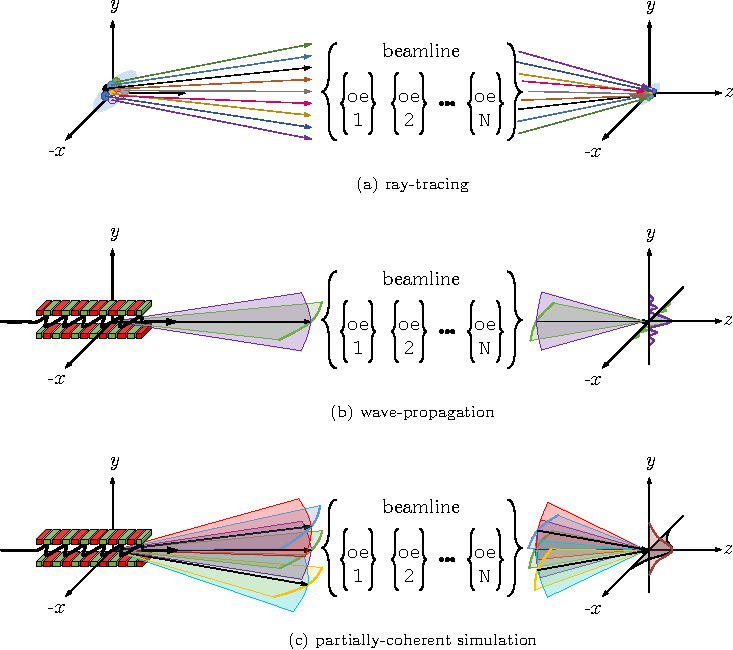
\includegraphics[width=.65\linewidth]{figures/ch02/optical_simulation.pdf}}
    \caption[X-ray optical simulation methods]{X-ray beamline optical simulation methods based on the degree of spatial coherence. A beamline is composed of drift-spaces (free-space) and optical elements (OE). (a) ray tracing methods are more adequate for cases where the degree of spatial coherence is low $\big(|j(\textbf{r}_1,\textbf{r}_2)|\approx0\big)$. (b) When the degree of coherence is close to unity $\big(|j(\textbf{r}_1,\textbf{r}_2)|\approx1\big)$ wave-propagation methods are better suited, as they account for diffraction effects. (c) partially-coherent simulation surpasses the accuracy of pure ray tracing or wave-propagation for cases where $0\ll|j(\textbf{r}_1,\textbf{r}_2)|\ll1$.}
    \label{fig:simulation_methods}
\end{figure}
%-------------------------------------------------------------------------
%-------------------------------------------------------------------------
\subsection{Ray-tracing}\label{sec:ray_tracing}
%-------------------------------------------------------------------------
%-------------------------------------------------------------------------
 For the cases where synchrotron radiation has low spatial coherence, that is, the complex degree of spatial coherence $|j(\textbf{r}_1,\textbf{r}_2)|\approx0$ for a pair of points near opposed edges of the beam footprint, ray-tracing techniques are often employed. The radiation source is simulated by Monte-Carlo sampling of the photon-beam phase-space\footnote{Three spatial coordinates, two transverse angles to describe direction, and the electron-beam energy - the electrons in a storage ring have a Gaussian distribution around a central design energy. The statistical emission of photons is the cause of a change of electron energy leading to energy spread within the electron beam [\cite[\textit{8.3.1}]{Wiedemann2015}].} described by specific numerical models [\cite{Canestrari2013}] and each photon sampled from the source is transported through the beamline using geometrical optics\footnote{Geometric optics is the limit of the physical optics theory when $\lambda$ goes to zero [\cite[\textit{§1.3.C} \& \textit{§2.3}]{Saleh2019}]. In free-space rays propagate in a straight line and have their direction changed by interacting with optical elements. By adding to this pure geometrical model some physical properties, namely, polarisation, intensity and wavelength, it is possible to account for several optical elements based on specular reflection, refraction and diffraction.}. The propagated rays are accumulated at the observation plane. To generate enough statistics and allow the method to converge, several thousands of rays are typically used - cf. Fig.~\ref{fig:simulation_methods}(a). Ray-tracing is a simple and extremely powerful technique for calculating the main characteristics of the photon beam (size, divergence, photon distribution) at every plane along the beamline when diffraction effects are negligible.

%-------------------------------------------------------------------------
%-------------------------------------------------------------------------
\subsection{Wave propagation}\label{sec:wave_propag}
%-------------------------------------------------------------------------
%-------------------------------------------------------------------------

The other extreme is the fully coherent case, that is $|j(\textbf{r}_1,\textbf{r}_2)|\approx1$ for any two pair of points $\textbf{r}_1$ and $\textbf{r}_2$ inside the beam footprint. This regime is often prone to diffraction effects and the framework for dealing with those is best given by wave-propagation, which follows physical optics principles - cf. §\ref{sec:physical_optics}~-~\textit{\nameref{sec:physical_optics}}. The X-ray source can be simply approximated by any solution of the Helmholtz equation (Eq.~\ref{eq:Helmholtz}) or its paraxial form given by Eq.~\ref{eq:Helmholtz_paraxial}. The most commonly used solutions are: the plane wave (Eq.~\ref{eq:planewave}), the spherical wave (Eq.~\ref{eq:spherical}), the parabolic wave (Eq.~\ref{eq:parabolic}) and the Gaussian beam (not covered here). Alternatively, the wavefront emerging from any accelerator-based X-ray source described by an arbitrary magnetic field can be calculated [\cite{Chubar1995, Chubar2001}]. This wave-field can then be propagated in the free-space between the optical elements using the diffraction integrals (cf. Eqs.~\ref{eq:Huygens-Fresnel},  \ref{eq:Fresnel} or \ref{eq:Fraunhofer}). The interaction between the wave and optical elements in the beamline is done by the calculation of the appropriate transmission element\footnote{In addition to the theory describing the propagation of X-rays in the matter (§\ref{sec:thin_element}~-~\textit{\nameref{sec:thin_element}}) a variety of optical elements can be simulated within the wave optics by being able to describe them adequately as transmission elements, similar to a transfer function in signals and systems theory - cf. [\cite{Canestrari2014, Li2017}].}. After the said wave is propagated to the observation plane, the intensity and phase can be calculated. 

%-------------------------------------------------------------------------
%-------------------------------------------------------------------------
\subsection{Partially coherent simulations}\label{sec:partially_coherent}
%-------------------------------------------------------------------------
%-------------------------------------------------------------------------

When doing optical design for X-ray beamlines in synchrotron radiation facilities, there are several cases of interest that are neither well approximated by $|j(\textbf{r}_1,\textbf{r}_2)|\approx0$ nor by $|j(\textbf{r}_1,\textbf{r}_2)|\approx1$ for a pair of points near opposed edges of the beam footprint. Using pure ray-tracing or a single-wave-field propagation to those partially-coherent cases may lead to inaccurate results [\cite{SanchezdelRio2019}]. With varying accuracy, several methods can account for  partially-coherence effects.

%-------------------------------------------------------------------------
%-------------------------------------------------------------------------
\subsubsection*{Hybrid methods}
%-------------------------------------------------------------------------
%-------------------------------------------------------------------------

One class of methods is based on the so-called hybrid methods mixing elements of ray-tracing and wave propagation simulations [\cite{Semichaevsky2001}]. One common approach is to simulate the geometric effects from optical elements with ray-tracing and their diffraction contributions\footnote{Diffraction contributions are usually due to beam clipping by either physical acceptance of an optical element or slits and optical errors.} with wave optics. The diffraction caused by the optical elements is then integrated into ray-tracing by numerical convolution and sampling the calculated wave-front with rays [\cite{Shi2014}]. Another approach is to take into account the optical path followed by individual rays and asserting to them a phase and interpreting them as a localised phase of the wave-front. If sampling is sufficiently high, it is possible to reconstruct a wave-front. These special rays are propagated through the beamline using ray-tracing techniques and are added coherently\footnote{Taking into account their relative phase.} at the observation plane [\cite{Keller1962}].

%-------------------------------------------------------------------------
%-------------------------------------------------------------------------
\subsubsection*{Physical-optics-based methods}
%-------------------------------------------------------------------------
%-------------------------------------------------------------------------

A second class of methods involves purely wave-front propagation methods. The radiation from the X-ray source can be decomposed in orthogonal modes. These can be propagated though the beamline using the physical optics principles described in §\ref{sec:physical_optics}~-~\textit{\nameref{sec:physical_optics}}. Once the modes are propagated to the observation plane, they can be added in intensity\footnote{cf. Eqs.~\ref{eq:MCF}, \ref{eq:CSD} and \ref{eq:CMD} evaluated for $\textbf{r}=\textbf{r}_1=\textbf{r}_2$ and $\tau=0$.}. X-rays from undulators are commonly decomposed into Gaussian-Schell modes
[\cite{Coisson1997, Singer2011}], which becomes less accurate when dealing with ultra-low emittance machines. More recently, different factorisations have been proposed to accurately represent beams in low-emittance machines [\cite{Lindberg2015, Glass_2017}].

Alternatively, the fact that for high energies the emission from the electrons is uncorrelated can be explored. Each individual electron in a bunch has a different initial condition in terms of position $s=(x_e,y_e,z_e)$, direction $s'=(x'_e,y'_e)$ and energy $\gamma_e$. These electrons spread in the 6D phase-space according to a probabilistic distribution\footnote{The distribution $f(s,s',\gamma_e)$ is intimately connected to the nature of the X-ray source.} $f(s,s',\gamma_e)$ in phase-space such as $\int f(s,s',\gamma_e)~\mathrm{d}x_e\mathrm{d}y_e\mathrm{d}z_e\mathrm{d}x'_e\mathrm{d}y'_e\mathrm{d}\gamma_e=1$. The multi-electron-emission method for partially coherent simulations is based on individually calculating the synchrotron radiation emission of several electrons subjected to the initial conditions sampled from $f(s,s',\gamma_e)$ passing through an arbitrary magnetic field describing the X-ray source [\cite{Chubar1995}]. Each resulting electric field is then propagated through the beamline until the observation point, where the contributions from different electrons are added in intensity. The function $f(s,s',\gamma_e)$ should be statistically well-sampled (Monte-Carlo methods) to guarantee convergence. This multi-electron-emission method was first proposed and implemented by [\cite{Chubar2011}]. This method is shown in Fig.~\ref{fig:simulation_methods}(c).

%-------------------------------------------------------------------------
%-------------------------------------------------------------------------
\subsubsection*{Other methods}
%-------------------------------------------------------------------------
%-------------------------------------------------------------------------

A third class of methods is based on the propagation of the correlation functions\footnote{cf. §\ref{sec:optical_coherence}~-~\textit{\nameref{sec:optical_coherence}}.} through the beamline with methods resembling the ones from physical optics. The theory for such is described in [\cite{Parrent1959}] and [\cite[\textit{§4.4}]{Mandel1995}]. However, these methods are, at the time of this writing, not very commonly applied to X-ray optical simulations due to being very computationally expensive [\cite{Meng2015, Meng2017, Ren2019}] and are certainly not made available on any common software for X-ray optical simulations. $\blacksquare$

\addcontentsline{toc}{section}{References}
\printbibliography[heading=subbibliography]
\end{refsection}

 \cleardoublepage
\begin{refsection}
%-------------------------------------------------------------------------
%-------------------------------------------------------------------------
\chapter{X-rays as a branch of optics}\label{sec:x-ray_optics}
%-------------------------------------------------------------------------
%-------------------------------------------------------------------------

The X-rays have been consolidated as a branch of optics as early as the second half on the 1920's. This chapter presents \todo{...}. Although different optical elements are presented, the main focus of this work is given to refractive optics and more specificly, to X-ray refractive lenses. 

%-------------------------------------------------------------------------
%-------------------------------------------------------------------------
\section{The early days of X-ray optics}\label{sec:early_days}
%-------------------------------------------------------------------------
%-------------------------------------------------------------------------

Upon reporting the discovery of  X-rays in [\cite{Roentgen1896_ch3}], R\"{o}ntgen describes several properties, among them: a) that refraction cannot be conclusively observed and if the tested materials\footnote{The materials used were water, carbon disulfide, mica, ebonite and aluminium.} do refract the X-rays, their index of refraction cannot be larger than 1.05 [cf. \textit{§7} ibid.]; b) there is no noticeable regular reflection of the rays on none of the substances\footnote{Platinum, lead, zinc and aluminium.} examined [cf. \textit{§8} ibid.]; c) there is no observable interference phenomena [cf. \textit{§15} ibid.]; d) and finally, that the X-rays cannot be polarised\footnote{In fact, this observation is not accompanied by any experimental observation described in his manuscript, but it comes from him speculating about the X-rays nature: \textit{"If one asks oneself what the X-rays [...] actually are [...]. If the X-rays were to be ultraviolet light, this light should have the property: [...] c)
that it cannot be polarised by the usual means;"} [\cite[\textit{§17}]{Roentgen1896_ch3}].} by the usual means [cf. \textit{§17c} ibid.]. At the time of the discovery of the X-rays, their only likeness to light was that they propagated in a straight line in free-space. It took about 30 years for this to change.

Between the years of 1904 and 1906 polarisation in X-rays have been described and observed by C. Barkla [\cite{Barkla1904, Barkla1905, Barkla1906}]. Speculations and experiments regarding diffraction of X-rays start as early as the 1900's [\cite{Haga1903,Walter1908,Walter1909}], but it was not until the early 1910's that diffraction was successfully described [\cite{Laue1912}], observed [\cite{FriedrichKnippingLaue1912}] and modelled by what came to be known as the Bragg law of refraction [\cite{BraggW.H.1913}]. Early experiments aiming direct observation of refraction failed, but helped narrowing the index of refraction for the X-ray regime\footnote{C. Barkla's experiment aimed to measure the refractive index of potassium bromide for radiation of wavelength in the neighbourhood of 0.5~\r{A}.} to $0.999995\leq n \leq1.000005$ [\cite{Barkla1916}]. Further experimental observations of the Bragg's law started showing small deviations between expected and obtained values. These were first reported by \citeauthor{Stenstrom1919} in \cite*{Stenstrom1919}\footnote{The same kind of discrepancies were also observed and reported by \citeauthor{Duane1920} in \cite*{Duane1920} and \citeauthor{Siegbahn1920} in \cite*{Siegbahn1920} and \cite*{Siegbahn1921}.} and were attributed to the refraction of the X-rays as they penetrate the crystal\footnote{This was met by criticism from \citeauthor{Knipping1920} in \cite*{Knipping1920} \citep{Knipping1920}. However, as pointed out by A. \citeauthor{Compton1923} - cf. [\cite{Compton1923}], theoretical calculations made by \citeauthor{Ewald1920} in \cite*{Ewald1920} showed good agreement between experimental observations and the refraction hypothesis [\cite{Ewald1920}].}, limiting the index of refraction to $n\lesssim1$ [\cite[\textit{§3}]{Stenstrom1919}]. The experimental proof of the refraction of X-rays came in the mid-1920's with [\cite{Larsson1924}]. Being able to detect refraction was very important, as it directly allows to assume the existence of reflection and this can only occur if in a boundary surface there is a discontinuity in the indexes of refraction between the two media. If one of these phenomena is present, the the other one must too exist [\cite{Compton1928}]. Based on earlier reports about the discrepancies observed on the Bragg's law of refraction, A. \citeauthor{Compton1923} was able to estimate the glancing angles for several materials of the polished surfaces and demonstrate the total external reflection of X-rays [\cite{Compton1923,Prins1927}]. In fact, by the end of the 1920's, all fundamental characteristics\footnote{Reflection, refraction, diffraction, polarisation, diffuse scattering, emission and absorption spectra and the photoelectric effect are the essential characteristics of light considered by A. Compton in [\cite{Compton1928}].} of light have been found to be present for X-rays, making them undoubtedly a branch of optics [\cite{Compton1928}].  

%-------------------------------------------------------------------------
%-------------------------------------------------------------------------
\section{X-ray interactions with matter}\label{sec:interaction_with_matter}
%-------------------------------------------------------------------------
%-------------------------------------------------------------------------

\todo{Not finished - just some key points and ideas so I can resume writing here}
X-rays are electromagnetic radiation and as such, will primarily interact with the electronic clouds in atoms. X-rays, when being shone into matter, can either be scattered, absorbed or even not interact at all, and pass it completely. Scattering can be elastic (), that is, or inelastic (), meaning. Absorption may come either by ... or by, in this case ... .


From the point of view of optical design, there is rarely the need to go into too much depth regarding how X-rays interact with matter and such interactions can be microscopically described by either the index of refraction in the case of reflection and refraction; or by interference theory in the case of refraction by ordered array of atoms (Bragg diffraction) or any well-defined geometric structure (physical optics).

\todo{reproduce figure 1.13 from \cite{Attwood1999}.}

%-------------------------------------------------------------------------
% TODO list - chapter #2 - updated 17/06/2020
% Finish sections - this chapter is on hold to allow for writing chapter 4

%-------------------------------------------------------------------------
\subsection{The refraction index}\label{sec:refractive_index}
%-------------------------------------------------------------------------
%-------------------------------------------------------------------------

\todo{Discuss briefly the delta and beta and their show graphs from 5 to 100 kev (?) and also Figure 2.4.a of my master thesis showing the total absorption coefficients and a summation of coherent and incoherent scattering - for Be, Al, SU-8 and diamond (materials used in the thesis)}


%-------------------------------------------------------------------------
%-------------------------------------------------------------------------
\subsubsection*{Refraction}
%-------------------------------------------------------------------------
%-------------------------------------------------------------------------

\begin{figure}[t]
    \centering
    {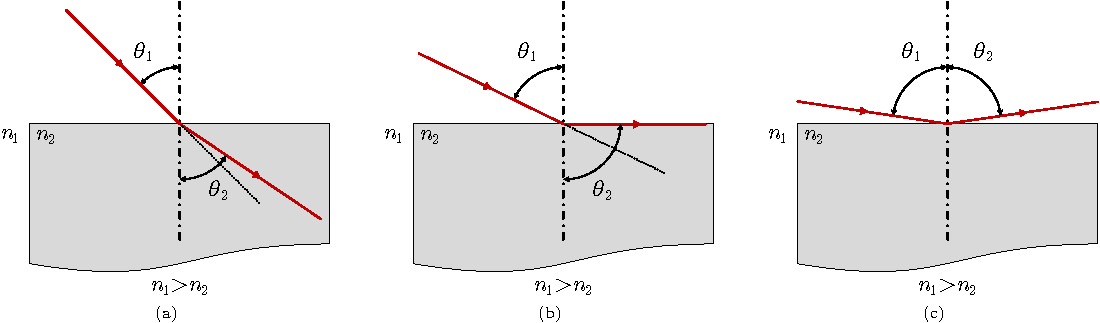
\includegraphics[width=0.7\linewidth]{figures/ch03/reflection_refraction.pdf}}
    \caption[Refraction and total external reflection in the X-ray regime]{Refraction and total external reflection in the X-ray regime.}
    \label{fig:reflection_refraction}
\end{figure}

The law of refraction\footnote{The observation of refraction, i.e. \textit{bending} of light as it changes medium, is as old as time, with one of the earliest written references from ca 150~\textsc{b.c.e.} in a philosophical poem "\textit{De Rerum Natura}" by Titus Lucretius Caro [\cite{Wilk2004}]. The first documented attempt to systematic describe refraction with a mathematical formulation and experimental data can be attributed to Claudius Ptolemy of Alexandria. His work, found in \textit{"Optics"} (from ca. 150~\textsc{c.e.}), presents studies on refraction at air-glass and air-water interfaces and arrives at a fairly accurate mathematical formulation for rays close to the optical axis (small angle approximation) [\cite{Kwan2002}], but still not the sine law found in any physics text book. The sine law found in most physics course books (Eq.~\ref{eq:refraction}) is commonly attributed to either Willebrord van Roijen Snell (obtained in 1621, but only published after his death by Christiaan Huygens on \textit{"Dioptrica"}, 1703) or Ren\'{e} Descartes (published in \textit{"La Dioptrique"}, annex to \textit{"Discours de la m\'{e}thode"} - 1637). The understanding and mathematical formulation can be traced back down to Abu Said al-Ala Ibn Sahl with \textit{"On the burning instruments"}, ~984 [\cite{Rashed1990}]; in a private communication between Johannes Keppler and Thomas Harriot, the latter discloses to Johannes Keppler he knew the sine law as early as of 1602 [\cite{Kwan2002,Lohne1956}]. In this work, equation \ref{eq:refraction} will be referred to as either the \textit{sine law} or \textit{law of refraction}.}:
\begin{equation}\label{eq:refraction}
    n_1\sin(\theta_1)= n_2\sin(\theta_2)
\end{equation}

%-------------------------------------------------------------------------
%-------------------------------------------------------------------------
\subsubsection*{Total external reflection}
%-------------------------------------------------------------------------
%-------------------------------------------------------------------------

The existence of refraction for a dielectric medium naturally implies the existence of reflection. 

%-------------------------------------------------------------------------
%-------------------------------------------------------------------------
\subsection*{Recommended literature}
%-------------------------------------------------------------------------
%-------------------------------------------------------------------------

An interesting account of the early days of X-ray optics is presented by [\cite{Compton1928}]\footnote{A more general account of the history of X-ray optics and science leading up to modern days is presented by [\cite[\textit{§1}]{Willmott2019}] and [\cite[\textit{§2}]{Jacobsen2019}].}. The interactions of X-ray with matter are presented with greater depth by [\cite{Als-Nielsen2011}] and [\cite[\textit{§1} - \textit{\textit{§3}}]{Attwood2016}].

%-------------------------------------------------------------------------
%-------------------------------------------------------------------------
\section{X-ray focusing optics}
%-------------------------------------------------------------------------
%-------------------------------------------------------------------------

Being able to identify the most basic optical phenomena in the X-ray regime naturally leads to exploiting those for the focusing of light.

%-------------------------------------------------------------------------
%-------------------------------------------------------------------------
\subsection{Diffractive optics}
%-------------------------------------------------------------------------
%-------------------------------------------------------------------------

This family of optical elements encompasses three large families of optical elements: crystals and multi-layer mirrors, where the main effect is\todo{...}; zone-plates\todo{...} and multi-layer Laue lenses (MLL)\todo{...}. A fourth incipient group if free-form diffractive optics for beam-tailoring \todo{cite: diffractive corrective optics}. 

%-------------------------------------------------------------------------
%-------------------------------------------------------------------------
\subsection{Reflective optics}\label{sec:reflec}
%-------------------------------------------------------------------------
%-------------------------------------------------------------------------
Mirrors \todo{...}

%-------------------------------------------------------------------------
%-------------------------------------------------------------------------
\subsection{Refractive optics}
%-------------------------------------------------------------------------
%-------------------------------------------------------------------------

Finally, the group of optical elements based on refraction of X-rays for focusing light (cf. Eq.~\ref{eq:refraction}) should be presented. Refractive X-ray optics comprises mainly lenses [\cite{Snigirev1996}], prisms in several arrangements [\cite{Cederstrom2000, Jark2004}] and most recently, free-form objects mainly for optical correction and beam-shaping [\cite{Seiboth2017, Zverev2017}]. From those, compound refractive lenses (CRLs) - as X-ray lenses are called - are by far the dominating refractive optical element in use throughout synchrotrons. In retrospective, they are the least mature\footnote{X-ray lenses were long believed to be unfeasible: low refraction index leads to unpractical focal lengths and the transmission of X-rays through matter faces strong absorption. In one of the early works on focusing and imaging with X-ray optics, P. Kirkpatrick and A. Baez stated that: \textit{"about one hundred lens surfaces in series would be required to bring the focal length down to one hundred meters. This would produce a cumbersome and very weak lens system of poor transparency. These discouraging considerations incline us toward other methods"}, using $f=R/\delta$, where $f$ is the focal length and $R$ is the refractive surface radius (cf. Eq~\ref{eq:Focus_simple}). The estimation shows values for $R=1$~cm, using beryllium lens at $\lambda=0.71$~\r{A}, K$_{\alpha}$ line of molybdenum [\cite{Kirkpatrick1948}]. On the following year, Kirkpatrick went on to say: \textit{"Although the X-ray lens is thus possible it has the disadvantages of high absorption and strong chromatic aberration, and so would probably be generally inferior to mirror systems"} [\cite{Kirkpatrick1949}]. It was not before 1991 that X-ray lenses would be reconsidered: in a scientific correspondence to the journal Nature, a Japanese group headed by S. Suehiro proposed the use of such elements for the forthcoming third generation light sources [\cite{Suehiro1991}]. Such idea was not met with enthusiasm by the X-ray optics community, who still considered such technologies to be impractical for focusing X-rays as it was made clear by A. Michette, who had written Nature a reply to Suehiro's communication. The text entitled \textit{"No X-ray lens"} criticises the idea of refractive optics for X-rays and lists the reasons why those were considered them unsuitable for focusing X-rays [\cite{Michette1991}]. In \textit{"Fresnel and refractive lenses for X-rays"} by B. X. Yang, written in 1992 and published in 1993, Yang revisited S. Suehiro's idea and proposed ways to overcome the strong absorption of such lenses by using a Fresnel lenses shape instead [\cite{Yang1993}], however those were at the time of complicated fabrication and were not given too much attention. The birth of the X-ray refractive lens as known today can be traced back to 1994, when T. Tomie filed a patent for X-ray lenses in Japan [\cite{Tomie1994}] - patents were also filed in US and Germany on the following year. His concept for X-ray lenses was introduced to the scientific community as poster on the \textit{XRM'96, Int. Conf. X-ray Microscopy and Spectroscopy}, held in W\"urzburg, Germany, in 1996. The concept was simple, but innovative: a series of drilled holes into a single substrate along a straight line. The proposed design increased mechanical robustness, overcame alignment issues, reduced absorption by placing the drilled holes close to each other and was relatively simple to be manufactured - although Tomie never went on to produce them [\cite{Tomie2010}]. Shortly after the presentation of the refractive lens to the scientific community at the XRM'96, the breakthrough came: A. Snigirev and other colleagues have produced the first compound refractive lens and have demonstrated its efficiency in focusing hard X-rays. It was only 100 years after the discovery of the X-rays that their focusing by refraction was experimentally demonstrated. This first experiment was performed at the European Synchrotron Research Facility (ESRF) in  Grenoble, France [\cite{Snigirev1996}]. The group used a very a similar approach as the one proposed by Tomie. This footnote was originally published as \textit{§3.1~-~Prelude} in [\cite{Celestre2017}].}, dating from the mid-1990's, while the use of diffractive focusing optics dates to the early 1930's and reflective optics to the late 1940's. 

%-------------------------------------------------------------------------
%-------------------------------------------------------------------------
\subsubsection*{The compound refractive lenses (CRL)\footnote{This section is partially based on the work originally published in [\cite{Celestre2020}].}}\addcontentsline{toc}{subsubsection}{-- The compound refractive lenses}
%-------------------------------------------------------------------------
%-------------------------------------------------------------------------

\begin{figure}[t]
    \centering
    {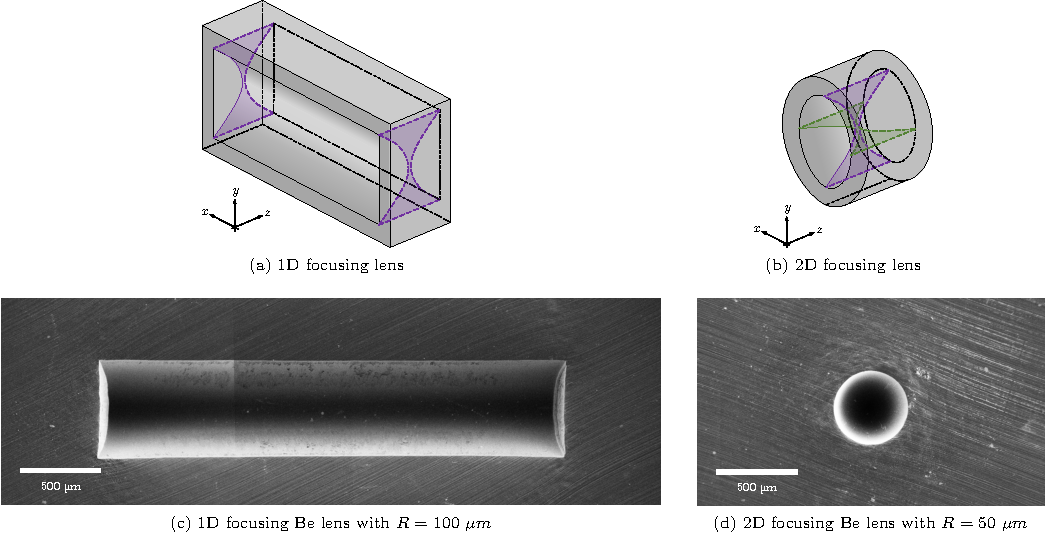
\includegraphics[width=.8\linewidth]{figures/ch03/1D2D.pdf}}
    \caption[1D and 2D focusing X-ray lenses]{1D (left) and 2D focusing (right) X-ray lenses. The top row shows a 3D rendering of such lenses with emphasis on the parabolic profile - shaded in purple is the vertical profile and in green, the horizontal profile. Bottom row shows scanning electron microscope (SEM) images of two Be lenses. Due to the limited field of view, image (c) is stitched, which explains the colour discontinuation on the left side of the image.} %SEM images were taken at the Institut Néel, in Grenoble, France; and are a courtesy of Raymond Barrett, X-ray optics group, ESRF.}
    \label{fig:1D2D_lenses}
\end{figure}

X-ray lenses may have different surface shape: in initial experiments a cylindrical surface was used [\cite{Snigirev1996, Protopopov1998}], which was soon replaced by a parabolic shape that almost completely removes geometrical aberrations [\cite{Elleaume1998, Lengeler1999}]. Parabolic lenses are the most used X-ray lenses in CRL as they can focus 1D (cylinder with parabolic section) or in 2D (paraboloid of revolution) - cf. Fig.~\ref{fig:1D2D_lenses}. It is worth noting, that although less usual, X-ray lenses can assume other shapes: an elliptical profile when focusing collimated beams [\cite{Evans-Lutterodt2003}], or a Cartesian oval for point-to-point focusing [\cite{SanchezdelRio2012}]. However, parabolic shapes always present a very good approximation to geometric focusing and reduce the geometrical aberrations to levels that are smaller than contributions from the fabrication errors and diffraction effects.

\todo{Note on materials, on CRL types and on manufacturing strategies.}
\todo{Graph with $\delta/\beta$ for common lens materials from 5kev to 100?}

%-------------------------------------------------------------------------
%-------------------------------------------------------------------------
\subsubsection*{-- CRL anatomy}
%-------------------------------------------------------------------------
%-------------------------------------------------------------------------

\begin{figure}[t]
    \centering
    {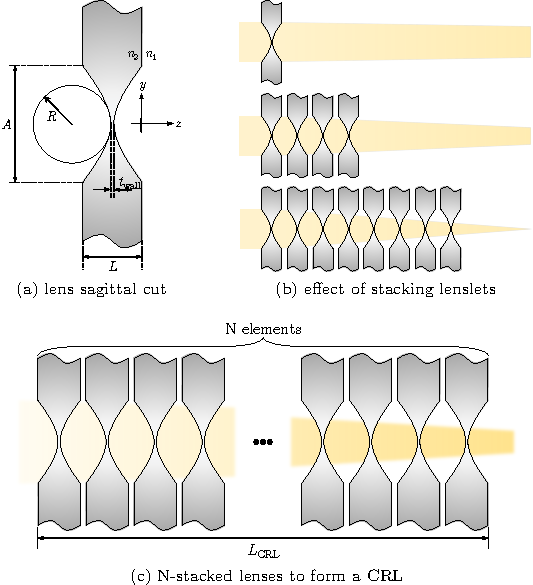
\includegraphics[width=0.5\linewidth]{figures/ch03/anatomy.pdf}}
    \caption[CRL anatomy]{(a) Sagittal cut of an X-ray lens showing its main geometrical parameters. This concave lens focuses X-rays in the $y$-direction if $n_1>n_2$. (b) A single X-ray lens refracts very weakly. To overcome this drawback - pointed out as early as the late 1940's [\cite{Kirkpatrick1948}] - lenses are usually stacked, hence "compound" in compound refractive lenses. (c) N-stacked lenses to form a CRL.}
    \label{fig:CRLs}
\end{figure}

Ideal parabolic X-ray lenses\footnote{Throughout this work, a single X-ray lens will be called a lenslet and two or more stacked lenses are referred to as compound refractive lens (CRL).} are usually defined by a small set of parameters as shown in Fig.~\ref{fig:CRLs}(a). These are: a) material, which, in conjunction with the operation energy defines the complex index of refraction $n$; b) apex radius of curvature ($R_x$ and $R_y$ for horizontal and vertical radii\footnote{For a 1D focusing lens, one of the radii goes to infinity on the non-curved surface. For a 2D focusing lens, the manufacturing goal is generally to produce lenses with $R_y=R_y=R$ to avoid astigmatism.}, respectively); c) lens thickness ($L$) or geometrical aperture ($A$); and d) distance between the apices of the parabolas ($\text{t}_{\text{wall}}$)\footnote{The web thickness ($\text{t}_{\text{wall}}$) is directly linked to the absorption and transmission of a X-ray lens, having no useful optical function. It should be kept as small as possible as to minimise absorption but as thick as necessary as to maintain the lenslet mechanical integrity. The exaggerated thinning of the web thickness leads to the risk or breaking the lens in brittle materials and shape deformation in ductile materials, deteriorating the lenslet performance [\cite{Lengeler1998}].}.

Firstly, one should start by defining the optical power $F=f^{-1}$ of a single refracting surface of radius $R$, where $f$ is its focal length. The index of refraction for the X-ray regime can be expressed as a complex number: $n = 1-\delta+i\cdot\beta$, with $\delta$ being the refraction index decrement and $\beta$, the absorption index - both strongly dependent on energy and material as discussed previously. With the X-ray beam moving along the positive $z$-direction on Fig.~\ref{fig:CRLs}, the refracting power of the vacuum/lens interface is given by:
\begin{equation}\label{eq:Focus_simple}
    F\equiv\frac{1}{f}=\frac{n_2-n_1}{-R}=\frac{\delta}{R}.
\end{equation}{}
Eq.~\ref{eq:Focus_simple} considers only the real part of the indices of refraction as this is the part that governs the focusing effect of the lenses. As illustrated by Fig.~\ref{fig:CRLs}(a), lenses are typically formed by two refracting surfaces of nominally the same radii. From paraxial optics, the total optical power of refracting surfaces in intimate contact is the sum of their powers. The same is valid for the cases where the distance between them can be ignored. Typical materials used for X-ray lenses have $10^{-7}\leq\delta\leq10^{-3}$ for their usual application energies [\cite{Serebrennikov2016}]. To overcome the weak refraction of a single element, several X-ray lenses are stacked [\cite{Tomie1994, Snigirev1996}]. Still, under the assumption of thin elements:
\begin{equation}\label{eq:CRL_classic}
    f_{\text{thin}\text{~CRL}} = \frac{R}{2N\delta},
\end{equation}{}
where the $2N$ comes from stacking $N$ lenslets with two refracting surfaces each, as shown in Fig.~\ref{fig:CRLs}(b). A correction factor can be added to Eq.~\ref{eq:CRL_classic} in order to account for the thick-element nature of the CRL, as proposed in [\cite{Kohn2003}]. The corrected focal length for a thick CRL is given by:
\begin{equation}\label{eq:CRL}
        f_{\text{CRL}} = \frac{R}{2N\delta}+\frac{L_{\text{CRL}}}{6}.
\end{equation}{}
This focal distance is taken from the middle of the CRL and $L_{\text{CRL}}$ is the CRL longitudinal size, that is, distance from the front surface of the first optical element to the back surface of the last lens - cf. Fig.~\ref{fig:CRLs}(c). The number of lenslets stacked in a CRL is mainly limited by absorption of the X-rays propagating within the lenses. 
\begin{figure}[t]
    \centering
    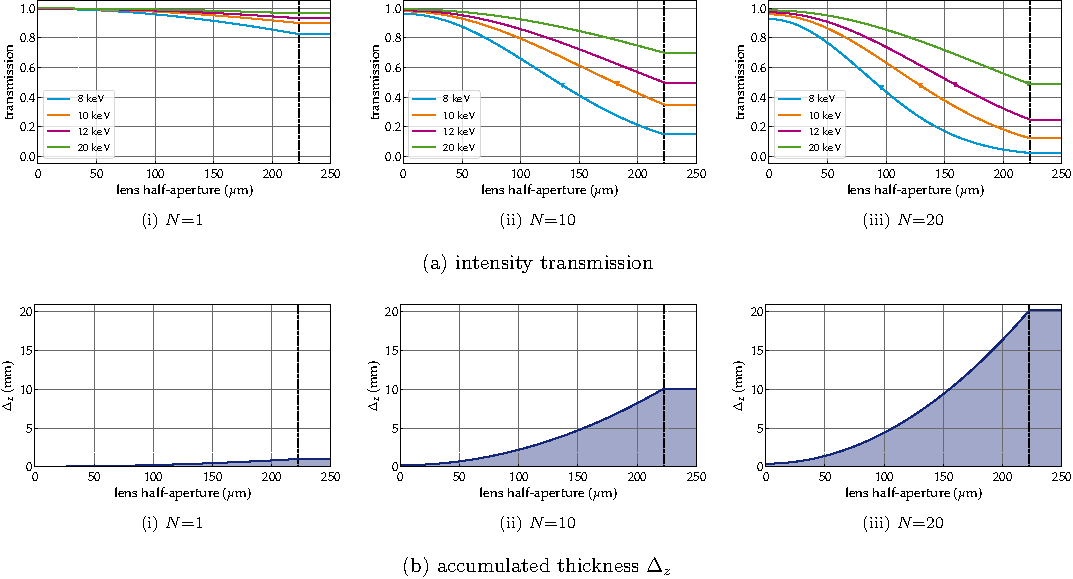
\includegraphics[width=1\linewidth]{figures/ch03/Aeff.pdf}
    \caption[Intensity transmission and accumulated thickness profile of CRLs]{(a) Normalised intensity transmission and (b) accumulated profile thickness for a CRL composed of ($\mathrm{i}$) 1, ($\mathrm{ii}$) 10 and ($\mathrm{iii}$) 20 2D-Beryllium lenses with nominal radius $R=50~\mu\text{m}$, geometric aperture $A_{\diameter}=445~\mu\text{m}$ and $t_\text{wall}=20~\mu$m at different photon energies (for the intensity profiles). Vertical dashed line represents the lens geometrical half-aperture. The triangles in (a) indicate the full width at half maximum (fwhm) for the cases where this value lies within the geometrical aperture.}
    \label{fig:EffectiveAperure}
\end{figure}
Another important parameter for optical design is the lens geometrical aperture $A$, as it provides an upper bound for the numerical aperture of the system and, ultimately, to the theoretical optical resolving power. Assuming a parabolic profile of the refracting surface, the lens geometrical aperture can be calculated as:
\begin{equation}\label{eq:A}
    A = 2\sqrt{(L-\text{t}_\text{wall})R},
\end{equation}{}
where $L$ is the lenslet thickness and $\text{t}_\text{wall}$ is the distance between the apices of the parabolas, commonly referred to as web thickness. For a 1D-focusing lenslet, the aperture related to the uncurved surface is limited only by manufacturing constraints and not the intrinsic lens parameters. Depending on the process used for lens production, it is convenient to isolate $L$ in Eq.~\ref{eq:A}:
\begin{equation}\label{eq:L}
    L = \frac{A^2}{4R}+\text{t}_\text{wall}.
\end{equation}{}
It is clear from Eqs.~\ref{eq:A} and \ref{eq:L} that for a parabolic surface, $A$ and $L$ are intertwined. More often than not, the maximum aperture $A$ is limited by the absorption from the lens thickness on the edge of the parabolic surface (lens active area). The geometrical aperture defined in Eq.~\ref{eq:A} is greater than or equal to the \textit{effective} lens aperture\footnote{There are several reported ways of defining the \textit{effective} lens aperture - [\cite{Kohn2017}] discusses and compares some of the different definitions. } as indicated by [\cite{Kohn2017}]. Figure~\ref{fig:EffectiveAperure} shows the transmitted intensity profile of a CRL composed of a different number of 2D-Beryllium lenses with nominal radius $R=50~\mu\mathrm{m}$ and circular geometric aperture $A_{\diameter}=445~ \mu\mathrm{m}$ at several energies. Unlike visible optics, where the transmitted intensity profile within the aperture, closely follows that of the illumination, the transmitted profile through a (stack of) X-ray lens(es) has strong absorption towards the edge, which defines the CRL as an apodised optical system.

% Note to myself: the critical angle limitation on the parabolic profile is not a real concern... aperture get's so large, that it makes no physically sense. Absorption is more pronounced. 

%-------------------------------------------------------------------------
%-------------------------------------------------------------------------
\subsubsection*{-- CRL modelling: ideal thin lens and single lens equivalent}
%-------------------------------------------------------------------------
%-------------------------------------------------------------------------

\begin{figure}[t]
    \centering
    {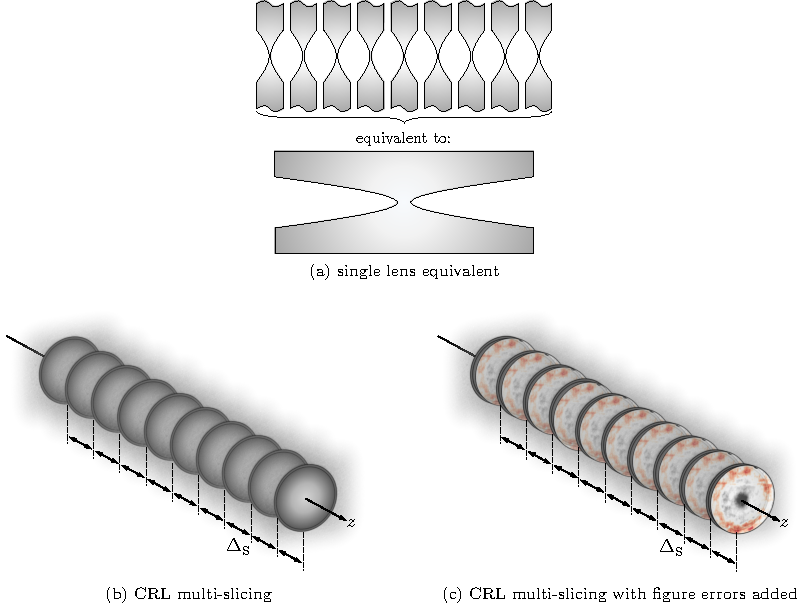
\includegraphics[width=0.7\linewidth]{figures/ch03/models.pdf}}
    \caption[Hierarchical CRL representation]{Hierarchical depiction of the CRL. (a) illustrates a single thin element equivalent of several lenslets. This representation accounts for net refraction and absorption in one transmission element but ignores intra-lens spacing. (b) multi-slice representation of a CRL. Here each lens of the stack is represented individually by one transmission element. Those are separated by a drift space corresponding to the typical distance between elements ($\Delta\text{s}$). (c) Not only can the CRL be represented as a series of thin elements separated by drift spaces, but also figure errors can be added. They are placed directly after the thin element representing a single X-ray lens.}
    \label{fig:models}
\end{figure}

At any point inside the geometric aperture of a single paraboloidal X-ray lens, the projected thickness $\Delta_z$ can be calculated as:
\begin{equation}\label{eq:ProjecThick}
    \Delta_z(x,y) = 
     \begin{cases}
      \cfrac{x^2}{R_x}+\cfrac{y^2}{R_y}+\text{t}_\text{wall}, &\quad\forall~(x,y) \in A,\\
      L, &\quad\text{otherwise}.
     \end{cases}
\end{equation}
If the lens being modelled is a 1D focusing element, that is a cylinder with parabolic section, one of the radii goes to infinity to account for the non-curved surface. The geometric aperture in this direction is not given by Eq.~\ref{eq:A}, but arbitrarily chosen (cf. Fig.~\ref{fig:1D2D_lenses}). Eq.~\ref{eq:ProjecThick} can be substituted into Eqs.~\ref{eq:aux_funcs_transa} and \ref{eq:aux_funcs_transb} to retrieve the complex transmission element expression for an X-ray lens:
\begin{eqnarray}\label{eq:TE_singlelens} % https://tex.stackexchange.com/questions/74129/piecewise-function
    \mathrm{T}_{\text{single lens}}(\Delta_z)~\bullet =
    \exp{\bigg(-\frac{2\pi}{\lambda}\beta\Delta_z \bigg)}
    \times\exp{\bigg(-i\frac{2\pi}{\lambda}\delta\Delta_z \bigg)} \bullet.
\end{eqnarray}{}
Eq.~\ref{eq:TE_singlelens}, the single lens model, accounts for the absorption (first exponential) and phase shift (second exponential) \footnote{The constant phase shift induced by $t_\text{wall}$ in Eq.~\ref{eq:TE_singlelens} (cf. Eq.~\ref{eq:ProjecThick}) can often be disregarded, as it impinges a constant phase to the wave-field.}. The complex transmission representing a CRL composed of $N$ elements is, thus, represented by:
\begin{equation}\label{eq:TE_CRL}
    \mathrm{T}_{\text{CRL}}(\Delta_z)~\bullet = \big[\mathrm{T}_{\text{single lens}}(\Delta_z)\big]^{N} \bullet,
\end{equation}{}
which is equivalent to multiplying $\Delta_z$ by $N$ in Eq.~\ref{eq:TE_singlelens}. The model represented by Eq.~\ref{eq:TE_CRL} will be referred to as the single lens equivalent. This model represents a lens stack by a single transmission element with equivalent focal distance and the projected thickness of all the $N$ single lenses as shown in Fig.~\ref{fig:models}(a).

%-------------------------------------------------------------------------
%-------------------------------------------------------------------------
\subsubsection*{-- CRL modelling: multi-slicing representation}
%-------------------------------------------------------------------------
%-------------------------------------------------------------------------

For a CRL composed of a very high number of lenslets, the single-lens equivalent approximation (Eq.~\ref{eq:TE_CRL}) may not be adequate to correctly represent such optical systems mainly due to the thick\footnote{In terms of optical element modelling.} nature of the stack  - evidenced by Eq.~\ref{eq:CRL}; and due to the progressive focusing inside the CRL [\cite{Schroer2005}] - exaggerated in Fig.~\ref{fig:CRLs}. For such cases, it is possible to adapt the multi-slicing (MS) techniques\footnote{cf. \textit{The Multi-slice approximation} in \S\ref{sec:thin_element}~-~\textit{\nameref{sec:thin_element}}.} for the calculation of the transmission of a wavefront through a CRL. Unlike the methods described by [\cite{Paganin2006}] and most recently, by [\cite{Li2017}] and [\cite{Munro2019}], where a single weakly-scattering optical element is sliced into several slabs, it is sufficient for most practical cases to break down a CRL into its lenses as shown in  Fig.~\ref{fig:models}(b). This can be justified by the fact that at their typical operation energy, the materials used for lens manufacturing have a very low $\delta$ [\cite{Serebrennikov2016}], rendering the individual lenslets a weak focusing element where the projection approximation holds [\cite{Protopopov1998}]. The complex transmission representation of a CRL based on the MS approach is given by:

\begin{equation}\label{eq:TE_CRL_MS}
    \mathrm{T}_{\text{CRL-MS}}(\Delta_z)~\bullet = \mathrm{T}_{\text{single lens}}(\Delta_z)\cdot\big[\mathcal{D}({\Delta}\text{s})\cdot\mathrm{T}_{\text{single lens}}(\Delta_z)\big]^{N-1}\bullet,
\end{equation}{}
where $\mathcal{D}({\Delta}\text{s})$ is the operator formulation of the Fresnel free-space propagation over a distance $\Delta\text{s}$ (distance between the centre of two adjacent lenses) - cf. Eqs.~\ref{eq:MS} and \ref{eq:Fresnel_operator}. 

Eq.~\ref{eq:TE_CRL_MS} represents a wavefront $\bullet$ modified by a single lens complex transmission $\mathrm{T}_{\text{single lens}}$, followed by free-space propagation $\mathcal{D}({\Delta}\text{s})$ over a distance $\Delta \text{s}$. The multiplication of the resulting electric field by the transmission element and subsequent free-space propagation is done $(N-1)$ times until the $N^{\text{th}}$ lens is reached and the last element of the lens stack is accounted for.

Optical imperfections measured with high spatial resolution can be readily converted into a transmission element by direct application of Eq.~\ref{eq:transmission_operator} to the height profile, provided it is a 2D map of the phase defects. In this case, the height profile will be the projected thickness of $\Delta_z(x,y)$ in the preceding equations. The MS model introduced earlier in this section can then be adapted to account for the phase errors of the individual lenses:
\begin{equation}\label{eq:TE_CRL_MS_ERR}
    \mathrm{T}_{\text{CRL-MS}}(\Delta_z)~\bullet = \mathrm{T}_{\text{imperfect lens}}(\Delta_z)\cdot\big[\mathcal{D}({\Delta}\text{s})\cdot\mathrm{T}_{\text{imperfect lens}}(\Delta_z)\big]^{N-1}\bullet,
\end{equation}{}
with:
\begin{equation}
    \mathrm{T}_{\text{imperfect lens}}(\Delta_z) = \mathrm{T}_{\text{figure errors}}(\Delta_z)\cdot\mathrm{T}_{\text{single lens}}(\Delta_z).
\end{equation}{}
This extended version of the MS model is shown in Fig.~\ref{fig:models}(c). In fact, the modelling of optical elements by means of  Eq.~\ref{eq:TE_CRL_MS_ERR} allows for the description of inhomogenities in the index of refraction within the lens as differences in material density and grain size [\cite{Lyatun2020}], inclusions and voids [\cite{Roth2014}], and even include effects of diffuse scattering/SAXS for a 2D map with very high spatial resolution [\cite{Paganin2019}].

%-------------------------------------------------------------------------
%-------------------------------------------------------------------------
\subsubsection*{-- CRL performance: diffraction limited focal spot}
%-------------------------------------------------------------------------
%-------------------------------------------------------------------------

Even an ideal and aberration-free finite optical element is not able to image a point-source to a point-like image. Limiting the extent of the focusing element by defining an aperture will induce diffraction effects on the wavefront and these will limit the smallest reachable focus spot size. The normalised response of the optical system to this point-like source input is called the point-spread-function (PSF). For a system with circular aperture and uniform amplitude across the exit pupil, the intensity of such focused beam at the image plane is proportional to a squared first-order Bessel function of the first kind (Airy pattern). The FWHM of the central cone is given by:
\begin{align}\label{eq:PSF}
    d = 1.22\lambda (1-M)\frac{f_{\text{CRL}}}{A},
\end{align}{}
where the $M$ is the magnification of the system, which goes to zero for a plane wave or a very distant source. Systems with nonuniform illumination at the pupil exit, in the case of the CRLs, an apodised systems approaching a Gaussian illumination, may present a different PSF shape depending on the truncation imposed by the aperture  (see Fig.~\ref{fig:PSF}). A very weakly truncated focusing system will have a Gaussian-shaped focal spot as little to no cropping occurs and therefore diffraction effects can be neglected. Increasing the truncation of the beam enhances diffraction effects from the geometric aperture. A strongly truncated focusing system will have a PSF that resembles the diffraction pattern in the far-field associated with the aperture of the system\footnote{The far-field diffraction pattern of a circular aperture is a squared first-order Bessel function profile while a square aperture will produce a 2D sinc-squared pattern [\cite{Guasti1993}].} [\cite{Mahajan1986}]. 

\todo{Figure with 2 graphs side by side: transmission (like Fig \ref{fig:EffectiveAperure}) and the horizontal cut of the PSF. 4 curves: 100\% transmisson on the edge of A, 75\%, 1$/e^2$ and 0}

%-------------------------------------------------------------------------
%-------------------------------------------------------------------------
\subsubsection*{-- CRL performance: transmission, gain and efficiency}
%-------------------------------------------------------------------------
%-------------------------------------------------------------------------

\todo{Look for that in the literature. That's commonly used by other authors - check for Tummlers and Benners PhD thesis}

%-------------------------------------------------------------------------
%-------------------------------------------------------------------------
\subsubsection*{-- CRL performance: tolerance conditions for aberrations}
%-------------------------------------------------------------------------
%-------------------------------------------------------------------------

Introducing errors to the optical system will reduce the peak intensity in the PSF [\cite[\textit{\S8.2}]{Mahajan2011}]. The ratio between the peak intensities of the aberrated- and non-aberrated PSF of a system with the same aperture and focal length is referred to as the Strehl ratio - cf. \S9.1.3 in [\cite{born_wolf1999}]. The optical aberrations on the exit pupil of an optical system can be described by the aberration function $\Phi(x,y)$, with the dimension of metres, which represents any deviation in shape from an ideal profile. For small aberration values, the Strehl ratio can be approximated\footnote{Eqs.~\ref{eq:Strehl}-\ref{eq:Mahajan} were obtained using a fully-coherent illumination of the optical system, however, defining the Strehl ratio as the ratio between the peak intensities of the aberrated- and non-aberrated optical under study transcends the nature of the illumination. A more complete derivation of the Strehl ratio (Eq.~\ref{eq:Strehl}) can be found in \S9.1.3 - \textit{A relation between the intensity and the average deformation of wave-fronts} in [\cite{born_wolf1999}].} by:
\begin{equation}\label{eq:Strehl}
    S_{\text{ratio a}}=\frac{I_{\text{aberrated}}}{I_{\text{aberration free}}}\approx1-\bigg(\frac{2\pi}{\lambda}\bigg)^2\Delta\Phi^2,
\end{equation}{}
where $\Delta\Phi$ is the standard deviation of the aberration function $\Phi(x,y)$. An important consequence of Eq.~\ref{eq:Strehl} is that the reduction in the peak intensity on the focal plane does not depend on the type of aberration nor the focal length of the optical system, but on its standard deviation across the exit pupil of the optical system [\cite{born_wolf1999}]. Alternative expressions to Eq.~\ref{eq:Strehl} are available in \S8.3 of [\cite{Mahajan2011}], namely:
\begin{align}\label{eq:Marechal}
    S_{\text{ratio b}}\approx\bigg[1-\bigg(\frac{2\pi}{\lambda}\bigg)^2\frac{\Delta\Phi^2}{2}\bigg]^2,
\end{align}
known as the Mar\'echal expression and:
\begin{align}\label{eq:Mahajan}
    S_{\text{ratio c}}\approx\exp{\bigg[- \bigg(\frac{2\pi}{\lambda}\bigg)^2\Delta\Phi^2\bigg]},
\end{align}
an empiric expression that fits better numerical results [\cite{Wetherell1980}]. However, for strong aberrations, there is no simple analytic expression to describe the relation between the Strehl ratio and the standard deviation of the aberration function $\Phi(x,y)$ [\cite{Kessler81}]. 

It is possible to define an arbitrary minimum acceptable value to the Strehl ratio when evaluating an optical element quality (tolerancing). This value depends on the final application and the desired performance. However, a value of $S_\text{ratio}\geq0.8$ is commonly found throughout literature as an indicator of a well-corrected optical system\footnote{This comes from historic reasons: both Rayleigh's $\lambda/4$ criterion for spherical aberrations (1879) and the extended Mar\'echal criterion for optical quality (1943) yield in a Strehl ratio of $\sim0.8$ [\cite{born_wolf1999}].}. Inserting $S_\text{ratio}\geq0.8$ in Eq.~\ref{eq:Strehl}, one obtains:
\begin{equation}\label{eq:MarechalCriterion}
    |\Delta\Phi|\leq\frac{\lambda}{14},
\end{equation}{}
which is known as the Mar\'echal criterion for optical quality. Equations~\ref{eq:Marechal}~and~\ref{eq:Mahajan} give similar limits: $\lambda/13.67$ and $\lambda/13.30$, respectively. In order to apply  Eq.~\ref{eq:MarechalCriterion} to the case of an X-ray lens, one makes use of Eq.~\ref{eq:aux_funcs_transb} with $\Delta\phi =\frac{2\pi}{\lambda}\delta\sigma_z=\frac{2\pi}{\lambda}|\Delta\Phi|$, where $\Delta\phi$ is the  standard deviation of the phase, and replaces the projected thickness\footnote{cf. \textit{The projection approximation} in \S\ref{sec:thin_element}~-~\textit{\nameref{sec:thin_element}}.} $\Delta_z$ with the standard deviation of the projected figure error $\sigma_z$:
\begin{align}\label{eq:ThickLim}
    \sigma_z &\leq \frac{\lambda}{14\delta}.
\end{align}{}
Equation \ref{eq:ThickLim} gives an upper limit to the standard deviation of accumulated figure errors for X-ray lenses in order to comply with the Mar\'echal criterion of tolerable wavefront aberrations, or in other words, to sustain a $S_\text{ratio}\geq0.8$. For a more complete discussion on the aberrated PSF, Strehl ratio and tolerance conditions for primary aberrations, refer to \S9 from [\cite{born_wolf1999}] and \S8 from [\cite{Mahajan2011}]. The limitations and applicability of the Maréchal criterion is presented in [\cite{Ross2009}].

%-------------------------------------------------------------------------
%-------------------------------------------------------------------------
\subsubsection*{-- CRL performance: chromatic aberrations}
%-------------------------------------------------------------------------
%-------------------------------------------------------------------------

The optical properties of the X-ray lenses are strongly dependent on the wavelength as both $\delta$ and $\beta$ have an energy dependency. This causes chromatic aberrations and limitations on the optical performance of the CRL under an X-ray beam with finite bandwidth. \todo{broadening of the focus spot}

The chromaticity of X-ray lenses can, however, be used favourably for X-ray harmonic rejection from insertion devices and coarse X-ray spectrum filtering [\cite{Vaughan2011, Polikarpov2014}]. $\blacksquare$
\addcontentsline{toc}{section}{References}
\printbibliography[heading=subbibliography]
\end{refsection}


 \cleardoublepage
\begin{refsection}
%-------------------------------------------------------------------------
%-------------------------------------------------------------------------
\chapter{Optical imperfections in refractive lenses}\label{sec:optical_imperfections}
%-------------------------------------------------------------------------
%-------------------------------------------------------------------------

To understand the impact of CRL on the optical design of complete beamlines, it is necessary to be able to simulate them realistically. The basic implementation of X-ray lenses is already available on the two most widespread beamline simulation tools: \textit{SHADOW} [\cite{SanchezdelRio2011}] and \textit{SRW} [\cite{Chubar1998}]. Both implementations, although based on different schemes, ray tracing [\cite{Alianelli2007}] and wave optics [\cite{Baltser2011}] respectively, are based on an ideal model combining refraction and absorption for the stacked lenses. Much has been done in terms of refining the modelling of ideal X-ray lenses [\cite{Umbach2008, SanchezdelRio2012, Osterhoff2013, Simons2017, Pedersen2018}] and, to a certain extent, the modelling of optical imperfections [\cite{Pantell2001, Andrejczuk2010, Gasilov2017, Osterhoff2017}]. Except for the work presented in [\cite{Roth2014}], investigating and simulating the inner structure of X-ray lenses, the present models consider mainly the lens shape and departure from a perfect parabolic shape. The majority of these models, however, is not publicly available, nor are readily compatible with standard beamline simulations suits like \textit{SHADOW} and \textit{SRW}. Another bottle-neck to the current literature or computer codes for simulating CRLs is that they do not include the data from real lenses metrology, as is routinely done for X-ray mirrors simulations [\cite{SanchezDelRio2016}], which undermines the inclusion of CRLs in simulations of complete beamline configurations in combination with other optical elements.

The modelling and functions presented here\footnote{This first section in this chapter, \S\ref{sec:describing_modelling}~-~\textit{\nameref{sec:describing_modelling}}, is partially based on the work originally published in [\cite{Celestre2020b}].} are based on the framework of physical optics (cf. \S\ref{sec:physical_optics}~-~\textit{\nameref{sec:physical_optics}}) and are tailored to be used transparently with SRW [\cite{Chubar1998}], which already provides a model for the CRL [\cite{Baltser2011}] - this basic ideal model combines refraction and absorption for the stacked lenses; optical imperfections from material inhomogeneities (voids, impurities) were later added [\cite{Roth2014}]. Expanding this model, we present the optical imperfections in refractive lenses in three different groups: \textit{i}-) misalignments of a single X-ray lens; \textit{ii}-) commonly encountered fabrication errors such transverse offsets as well as tilts of the individual parabolic sections; \textit{iii}-) and other sources of deviations from the parabolic shape modelled with either polynomial decomposition of error functions or by using metrology data. Each newly added feature is accompanied by a calculation of the residual thickness error, its impact on focusing by CRL and the beam caustic in the vicinity of the focal spot\footnote{All simulations shown throughout this chapter have similar conditions, that is, they model misalignments, fabrication errors or arbitrary residual errors to a single 2D-Beryllium lens with nominal radius $R=50~\mu\text{m}$, geometric aperture $A_{\diameter}=440~\mu\text{m}$ and $t_\text{wall}=20~\mu$m at 8~keV in fully-coherent simulations. The illumination is filament electron beam passing through a CPMU18 undulator with 111 magnetic periods with $\Lambda=18$~mm magnetic period and magnetic field $B=0.9863~$T - cf. \S\ref{sec:brilliance}~-~\textit{\nameref{sec:brilliance}}. The electron-beam parameters are the ones from the ESRF-EBS upgrade [\cite{orangebook}]. An ideal parabolic phase element with radius of curvature $R=-60~$m is placed 60~m downstream the radiation source to give the illumination a near-plane phase - cf. Eq.~\ref{eq:planewave}, so that the PSF and beam caustics can be calculated. The application of the presented modelling to partially-coherent simulations methods [\cite{Chubar2011}] is shown in \S\ref{sec:effect_optical_imperfections}~-~\textit{\nameref{sec:effect_optical_imperfections}}.}, which are summarised in Fig.~\ref{fig:Strehl}. Calculations presented in this chapter are merely illustrative and a systematic evaluation is presented in \S\ref{sec:effect_optical_imperfections}~-~\textit{\nameref{sec:effect_optical_imperfections}}. The code main functions implementing the ideal CRL and describing optical imperfections in refractive lenses are subsequently presented. The metrology technique used to obtain the phase errors that arise from material inhomogeneities (voids, impurities) and/or figure errors from the lens forming process, namely, X-ray speckle tracking, is discussed at length. After considerations on data processing and analysis, a selection of experimental data is discussed and corrective optics based on the metrology data is proposed. 


\begin{figure}[t]
    \centering
    {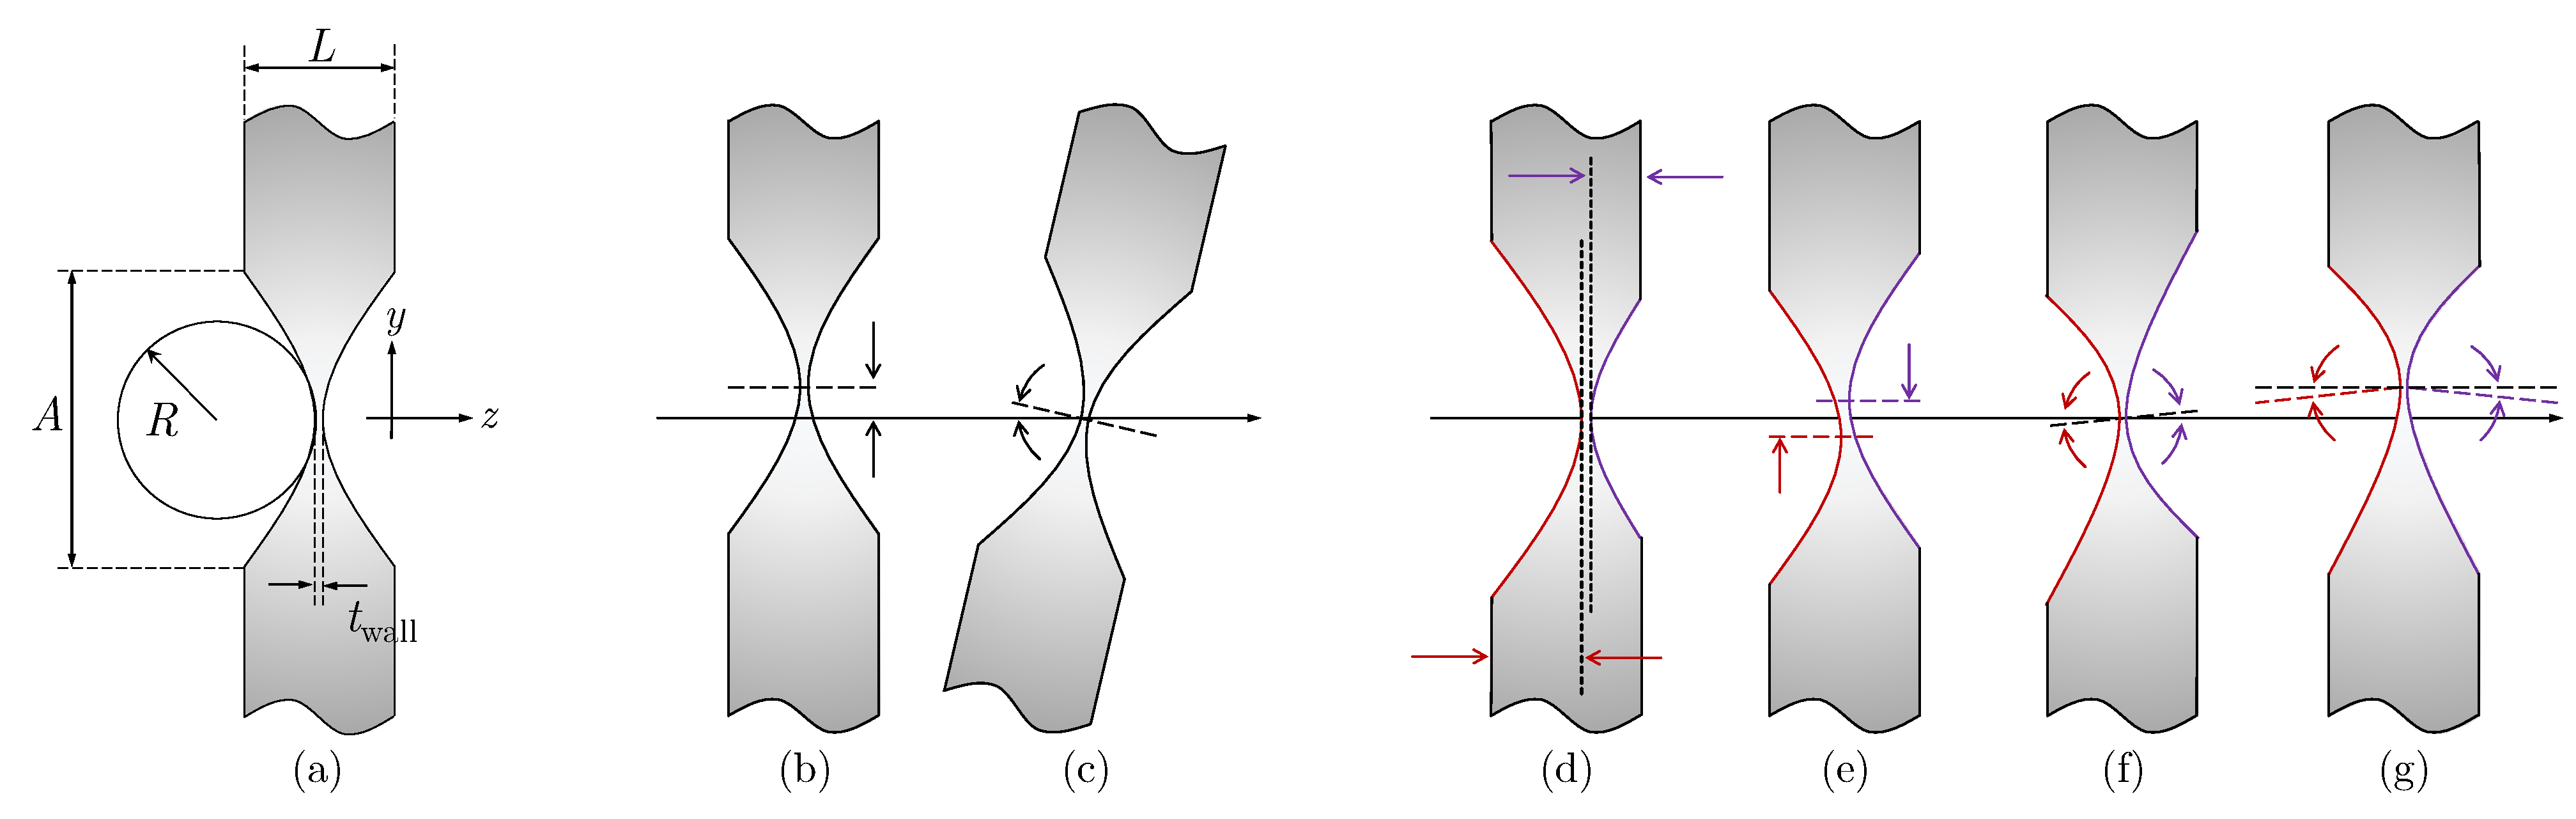
\includegraphics[width=1.\linewidth]{figures/ch04/lens_cuts.pdf}}
    \caption[Modelling misalignments and fabrication errors in CRLs]{(a) ideal lens for reference. Lens typical misalignments are the (b) transverse offset and the (c) tilt or a combination of both. Common fabrication errors include the (d) longitudinal offset of the parabolic section, (e) transverse offset of the parabolic section and (f)-(g) tilted parabolic sections.}
    \label{fig:lens_cuts}
\end{figure}

%-------------------------------------------------------------------------
%-------------------------------------------------------------------------
\section{Describing and modelling optical imperfections in refractive lenses}\label{sec:describing_modelling}
%-------------------------------------------------------------------------
%-------------------------------------------------------------------------

In the paraxial approximation, the parabolic shape for a refracting surface is generally regarded as the ideal shape\footnote{The shape of a focusing refracting surface can be derived from the Fermat's principle, but the parabolic shape is generally regarded as a good approximation. Large apertures are often necessary when very small focused beams are required, but increasing the geometric aperture of the optical element causes the parabolic approximation to under-perform. Several aspheric surface shapes for different focusing conditions were reported in [\cite{SanchezdelRio2012}] - cf. Fig~4. For a deeper discussion on aspheric surfaces in the context of optics, please, refer to [\cite{Schulz1988}].} for minimising aberrations. It is legit, then, to define as errors any deviation from this ideal parabolic form\footnote{Such definition, however, leaves out discrepancies in the radius of curvature $R$ (designed vs. \textit{de facto}) and the associated defocus it may cause. Discrepancies between designed and executed lenses may render them to be labelled as out-of-specification and may cause the system to under-perform, but are not deviations of the parabolic shape, provided the ideal parabolic shape takes into account the \textit{de facto} radius of curvature. Accounting for such discrepancies can be done using the ideal model described by the transmission element $\mathrm{T}_{\text{single lens}}(\Delta_z)$ (cf. Eq.~\ref{eq:TE_singlelens}) using the \textit{de facto} radius of curvature.} regardless of its origin. The phase errors induced by an ideal lens misalignment will be presented first, then the typical fabrication errors of bi-concave lenses will be presented shortly after. The misalignment and fabrications errors presented in this section were derived from the accumulated experience in handling beryllium and aluminium bi-concave embossed lenses, which are the most available throughout beamlines in diverse synchrotron facilities. However, the modelling presented here is generic and can be applied to a wide-range of CRL from diverse fabrication processes\footnote{cf. Table~1 from the supplementary material relative to [\cite{Roth2017}].}. Fig.~\ref{fig:ideal_CRL} shows the focusing performance of a single ideal 2D-Beryllium lens with nominal radius $R=50~\mu\text{m}$, geometric aperture $A_{\diameter}=440~\mu\text{m}$ and $t_\text{wall}=20~\mu$m at 8~keV using the SRW basic modelling. 
 \begin{figure}[t]
        \centering
        {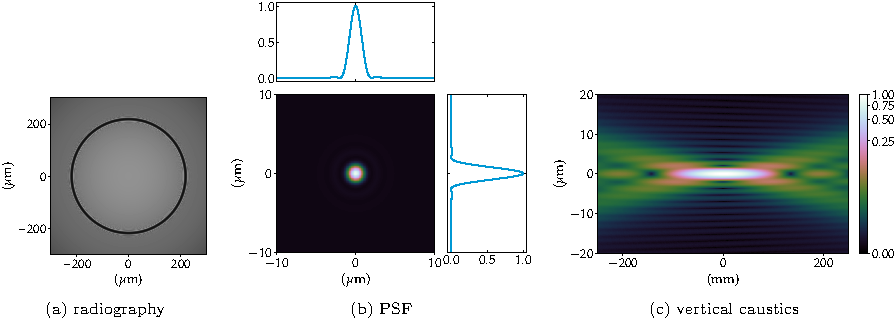
\includegraphics[height=4.19cm]{figures/ch04/CRL_ideal.pdf}}
        \caption[The ideal single X-ray lens]{Simulations of a single ideal 2D-Beryllium lens with nominal radius $R=50~\mu\text{m}$, geometric aperture $A_{\diameter}=440~\mu\text{m}$ and $t_\text{wall}=20~\mu$m at $8$~keV  - cf. Fig~\ref{fig:lens_cuts}(a). (a) phase-contrast image $150~$mm downstream the ideal lens, (b) point-spread function with cuts centred in $(0,0)$ and (c) the vertical beam caustics from $-250$~mm to $250$~mm in respect to the focal plane at $f=4.700~$m.} \label{fig:ideal_CRL}
\end{figure}


%-------------------------------------------------------------------------
%-------------------------------------------------------------------------
\subsection{Misalignments}\label{sec:misalignments}
%-------------------------------------------------------------------------
%-------------------------------------------------------------------------

Misalignments of optical systems are not optical errors \textit{per se} as they can be mitigated by ensuring proper alignment is done; they will, however, cause changes to the ideal parabolic phase profile if left uncorrected and will affect the optical performance of the system. Although aligning a CRL stack is possible\footnote{The possibility of realignment of the CRL depends on where and how they are installed in the beamline. If their installation is on a bulky transfocator [\cite{Vaughan2011}], their realignment is more difficult to be performed. However, when used as a final focusing element, enclosed in small casings or compact transfocators - cf. Fig.~3 in [\cite{Lengeler1999}] and [\cite{Kornemann2017, Narikovich2019}], their realignment can be done more easily.}, the individual lenslets usually cannot be aligned to each other, hence the interest in modelling such misalignments.

%-------------------------------------------------------------------------
%-------------------------------------------------------------------------
\subsubsection*{Transverse offset}
%-------------------------------------------------------------------------
%-------------------------------------------------------------------------

Shifting transversely a single element an transverse distance $(\Delta_x,\Delta_y)$ can be simply done by calculating $\Delta_z(x-\Delta_x,y-\Delta_y)$ in Eq.~\ref{eq:ProjecThick}. The shifted element is depicted in Fig.~\ref{fig:lens_cuts}(b). For a pair of coordinates $(x,y)$:
\begin{equation}\label{eq:ProjecThick_misaligned}
    \Delta_z(x-\Delta_x,y-\Delta_y) = 
        \begin{cases}
      \cfrac{(x-\Delta_x)^2}{R_x}+\cfrac{(y-\Delta_y)^2}{R_y}+\text{t}_\text{wall}, &\quad\forall~(x-\Delta_x,y-\Delta_y) \in A,\\
      L, &\quad\text{otherwise}.
        \end{cases}
\end{equation}   
Eq.~\ref{eq:ProjecThick_misaligned} is the ideal parabolic profile of a bi-concave lens given by Eq.~\ref{eq:ProjecThick} with its vertices centred around $(\Delta_x,\Delta_y)$. While a single transversely shifted lens considered on its own is innocuous, piling up several shifted lenses has impacts on the overall accumulated phase parabolic shape and resulting geometric aperture. Although the exact effect of relative misaligments between individual lenses on the phase of the wave-field depends on the distance between lenslets, the energy, footprint and divergence of the X-ray beam, some insight can be gained by considering the individual focusing elements as thin-optical elements in intimate contact. Consider $N$ stacked lenses transversely misaligned with their transverse distance to the optical axis given by $(\Delta_{x_j},\Delta_{y_j})$, with $j=1,~2,~...,~N$. Within the intersection of their geometric apertures, the accumulated thickness is given by:
% \begin{subequations}
\begin{align}\label{eq:ProjecThick_Nmisaligned}
    \Delta_{z_\Sigma}(x,y) &= \sum\limits_{j=1}^N \Delta_z(\Delta_{x_j},\Delta_{y_j})\nonumber\\
    &=\sum\limits_{j=1}^N \underbrace{\frac{x^2}{R_{x_j}}+\frac{y^2}{R_{y_j}}}_\text{(I)}
    -\underbrace{2x\frac{\Delta_{x_j}}{R_{x_j}} - 2y\frac{\Delta_{y_j}}{R_{y_j}}}_\text{(II)}
    +\underbrace{\frac{\Delta_{x_j}^2}{R_{x_j}}+\frac{\Delta_{y_j}^2}{R_{y_j}}+\text{t}_{\text{wall}_j}}_\text{(III)}.
\end{align}
The first term in Eq.~\ref{eq:ProjecThick_Nmisaligned}, ($\text{I}$) is a quadratic term and it indicates ideal focusing as in Eq.~\ref{eq:ProjecThick}. The residual terms ($\text{II}$) and ($\text{III}$) are a linear term in $x$ and $y$ and a constant offset term, respectively. The projected thickness and the phase are linearly proportional, so the residual accumulated thickness translates directly into residual accumulated phase and both terms can be used interchangeably - cf. Eq.\ref{eq:aux_funcs_transb}. The first residual term, i.e. ($\text{II}$), adds a linear phase to the wave-front and acts like a prism, not deforming the monochromatic wave-field, but redirecting it. At the focal plane, the image position is transversely shifted but no change to the intensity and phase profiles is added. Symmetrically shifted lenses\footnote{That is $\Delta_{x_m}=-\Delta_{x_n}$ or $\Delta_{y_m}=-\Delta_{y_n}$ for $m,n\in(1,~2,~...,~N)$.} make ($\text{II}$) goes to zero. The residual terms in ($\text{III}$) add a constant phase offset to the transmitted beam.  The effects of the transverse offset to a single X-ray lens are shown in Fig.~\ref{fig:shifted_CRL}.
\begin{figure}[t]
        \centering
         {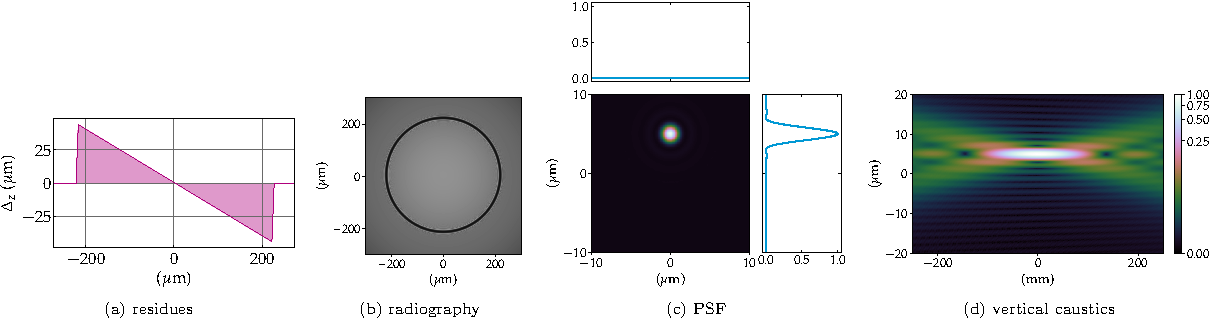
\includegraphics[height=4.19cm]{figures/ch04/shifted_CRL.pdf}}
        \caption[Effects of a transverse CRL offset]{Simulations of an ideal lens shifted by $\Delta_y=5~\mu$m - cf. Fig~\ref{fig:lens_cuts}(b). (a) Residual thickness, (b) phase-contrast image $150~$mm downstream the lens, (c) point spread function with cuts centred in $(0,0)$ and (c) the vertical beam caustics from $-250$~mm to $250$~mm in respect to the focal plane at $f=4.700~$m.} \label{fig:shifted_CRL}
\end{figure}


%-------------------------------------------------------------------------
%-------------------------------------------------------------------------
\subsubsection*{Tilted lens}
%-------------------------------------------------------------------------
%-------------------------------------------------------------------------
\begin{figure}[t]
        \centering
        {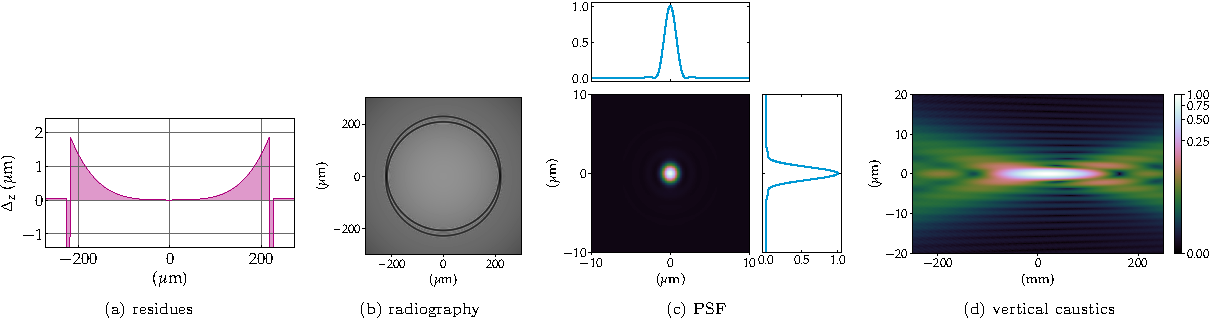
\includegraphics[height=4.19cm]{figures/ch04/tilted_CRL.pdf}}
        \caption[Effects of a CRL tilt]{Simulations of an ideal lens tilted by $\theta_x=1^{\circ}$ - cf. Fig~\ref{fig:lens_cuts}(c). (a) Residual thickness, (b) phase-contrast image $150~$mm downstream the lens, (c) point spread function with cuts centred in $(0,0)$ and (c) the vertical beam caustics from $-250$~mm to $250$~mm in respect to the focal plane at $f=4.700~$m. The profile shown in (a) is proportional to the 4$^{\text{th}}$ power of the lateral coordinates in the direction of the shift. This contributes for the elongation of the beam along the propagation direction and shift on the focal plane position as evidenced by (d), which is a typical sign of spherical aberrations.} \label{fig:tilted_CRL}
\end{figure}

When rotating a lens in space as shown in Fig.~\ref{fig:lens_cuts}(c) and calculating its projected thickness, it is helpful to decouple the rotation of the front and back surfaces. This can be done by defining a point cloud in Cartesian coordinates:
\begin{subequations}\label{eq:point_cloud}
    \begin{align}
    z_\text{front surface}(x-\Delta_x,y-\Delta_y) &=\frac{\Delta_z(x-\Delta_x,y-\Delta_y)}{2},\\
    z_\text{back surface}(x-\Delta_x,y-\Delta_y) &= -\frac{\Delta_z(x-\Delta_x,y-\Delta_y)}{2}
    \end{align}
\end{subequations}{}
where $\Delta_z(x-\Delta_x,y-\Delta_y)$ is given by Eq.~\ref{eq:ProjecThick_misaligned}. The projected thickness is given by:
\begin{align}\label{eq:point_cloud_thickness}
    \Delta_z(x,y) = z_\text{front surface}(x,y) - z_\text{back surface}(x,y),
\end{align}{}
provided those are calculated on the same grid $(x,y)$. A tilted lens can be described by rotation matrices in three dimensions. The transformation matrices allowing a rotation $\theta_{x,y,z}$ around each of the Cartesian axis are~[\cite{House2016}]:
\begin{subequations}\label{eq:affine}
    \begin{align}
        R_x &= \begin{bmatrix}
                            1 & 0 & 0 &0\\
                            0 & \cos\theta_x & -\sin{\theta_x}  &0\\
                            0 & \sin\theta_x & \cos\theta_x &0\\
                            0 & 0 & 0 &1
            \end{bmatrix}  &&(\small{\text{rotation around the $x-$axis}}),\\
            R_y &= \begin{bmatrix}
                            \cos\theta_y & 0 & \sin\theta_y &0\\
                            0 & 1 & 0 &0\\
                            -\sin\theta_y & 0 & \cos\theta_y &0\\
                            0 & 0 & 0 &1
            \end{bmatrix}  &&(\small{\text{rotation around the $y-$axis}}),\\
            R_z &= \begin{bmatrix}
                            \cos\theta_z & -\sin\theta_z & 0 &0\\
                            \sin\theta_z & \cos\theta_z & 0 &0\\
                            0 & 0 & 1 &0\\
                            0 & 0 & 0 &1
            \end{bmatrix}  &&(\small{\text{rotation around the $z-$axis}}).
    \end{align}
\end{subequations}{}
Matrix multiplication is associative, which implies that if multiple rotations are involved, that is $R_x, R_y$ and $R_z$ are applied to a set of points $(x,y,z)$, an equivalent rotation matrix $R_{\theta}=R_zR_yR_x$ can be calculated and then, applied to those points is space: 
\begin{align}\label{eq:affine2}
    [x_\theta,y_\theta,z_\theta,1]^\text{T} & = R_zR_yR_x[x,y,z,1]^\text{T},\nonumber \\
     & = R_\theta[x,y,z,1]^\text{T},
\end{align}{}
where $(x_\theta,y_\theta,z_\theta)$ are the transformed $(x,y,z)$ coordinates after the $R_{\theta}=R_zR_yR_x$ rotation and the $^\text{T}$ in Eq.~\ref{eq:affine2} represents transposed matrices. The rotations given by $R_{\theta}$ have to be applied to both the front and back surfaces of the lens independently, with their respective point clouds given by Eqs.~\ref{eq:point_cloud}. In order to calculate the projected thickness along the optical axis, the rotated front and back surfaces have to be recalculated on a common grid, which is done by two-dimensional interpolation of $(x_\theta,y_\theta,z_\theta)$ to the original $(x,y)$ grid. The associative property allows for considerable computation time reduction, as the rotation can be done applying a single equivalent rotation matrix as opposed to three individual rotations. On the other hand, matrix multiplication is not commutative and the order of operations matter and should be specified\footnote{The implementation of the affine transformations for rotating CRLs in space follow the order: rotation around the $x-$axis ($R_x$), rotation around the $y-$axis ($R_y$) and then, rotation around the $z-$axis ($R_z$).}$^{,}$\footnote{For a deeper discussion on the properties of the affine transformations, coordinates systems and quaternions, please refer to appendices \textit{C}-\textit{E} in [\cite{House2016}].} when rotating a point cloud. Equations~\ref{eq:affine} have their pivot point centred in the origin of their axis, that is, around $(x,y,z)=(0,0,0)$ in Cartesian coordinates. It is possible to define arbitrary pivot points with a combination of translations and rotations. Tilting an optical element in space will introduce aberrations to the beam propagation and its focusing\footnote{The interest in tilted optical elements and compensation is an active field, as evidenced by the literature on that subject - cf. [\cite{Guizar-Sicairos2011,Zhou2019,Ali2020}].}. This is evidenced by the residual accumulated thickness in projection approximation shown in Fig.~\ref{fig:tilted_CRL}. It is also possible to see how the two surfaces (back and front) do not overlap, causing a slight reduction in the geometric aperture area, which is evidenced by the discontinuities in Fig.~\ref{fig:tilted_CRL}(a).

%-------------------------------------------------------------------------
%-------------------------------------------------------------------------
\subsection{Fabrication errors}\label{sec:fabrication}
%-------------------------------------------------------------------------
%-------------------------------------------------------------------------

Modelling the typical misalignment of X-ray lenses implies calculating the lateral displacements and rotations in space of an ideal X-ray lens. However, bi-concave lenses may also present misalignments between the front and back focusing surfaces, these are closely related to the manufacturing processes involved in the lens production. Here, the front and back focusing surfaces are treated independently, allowing to model longitudinal and transverse misalignments as well as tilts of the front and back focusing surface concerning the optical axis.


%-------------------------------------------------------------------------
%-------------------------------------------------------------------------
\subsubsection*{Longitudinal offset of the parabolic section}
%-------------------------------------------------------------------------
%-------------------------------------------------------------------------
Longitudinal offsets of the parabolic portions of a bi-concave X-ray lens appear when, for the same radius of curvature $R$, one parabolic portion is deeper than the other one - cf. Fig.~\ref{fig:lens_cuts}(d). The first eminent observation if that front and back surfaces will have different geometric apertures along the focusing direction. The new geometric aperture of the longitudinally offset parabolic profile can be calculated as:
\begin{equation}\label{eq:A_2}
    A_{\text{offset}} = 2\sqrt{[L-(\text{t}_\text{wall}+2\cdot\text{offset})]R},
\end{equation}{}
where a positive offset increases the apparent web thickness of the half lens to $\text{t}_\text{wall}/2+\text{offset}$ and decreases the geometric aperture for a fixed lens thickness. The aperture given by $ A_{\text{offset}}$ and the apparent web thickness are used in Eq.~\ref{eq:point_cloud_thickness} (cf. Eqs.~\ref{eq:ProjecThick_misaligned} and \ref{eq:point_cloud}) when calculating the projected thickness.
Longitudinal offsets do not affect the parabolic accumulated shape of a single lens and, consequently, do not impose any optical imperfection to an optical system based on such lenses. However, they are often encountered in real lenses\footnote{Specially in embossed lenses, where different penetration depths of the punches often lead to asymmetric lenses.} and merit the implementation in the lens modelling. Fig.~\ref{fig:longitudinal_offset} shows the simulated profile and a radiography of a real lens showing the effects of the longitudinal offset of the parabolic section.

\begin{figure}[t]
        \centering
        {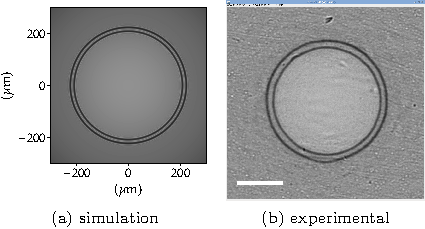
\includegraphics[height=3.cm]{figures/ch04/longitudinal_offset.pdf}}
        \caption[Effects of the longitudinal offset of the parabolic section]{(a) Simulated and (b) measured phase-contrast image of a single of a 2D-Beryllium lens with nominal radius $R=50~\mu\text{m}$ with designed geometric aperture $A_{\diameter}=440~\mu\text{m}$. The scale bar in (b) is worth $200~\mu$m.} \label{fig:longitudinal_offset}
\end{figure}

%-------------------------------------------------------------------------
%-------------------------------------------------------------------------
\subsubsection*{Transverse offset of the parabolic section}
%-------------------------------------------------------------------------
%-------------------------------------------------------------------------

Although parallel to the optical axis, it is possible that the parabolic surfaces axes are not collinear. This is shown in Fig.~\ref{fig:lens_cuts}(e). The modelling of the transverse offset of the front or/and back surfaces of a lens concerning the optical axis is done by calculating the net offset of each surface, that is the sum of lens transverse offset with the front or/and back surface transverse offset, and applying it to Eqs.~\ref{eq:point_cloud} when calculating Eq.~\ref{eq:point_cloud_thickness}. The effects on the residual accumulated phase of non-collinear parabolic surfaces are the same as the one described in the section \textit{Transverse offset} from \S\ref{sec:misalignments}~-~\textit{\nameref{sec:misalignments}}, that is, the presence in the residual phase of a linear and a constant term, which can be seen in Fig.~\ref{fig:offset_fs_CRL}.


\begin{figure}[t]
        \centering
        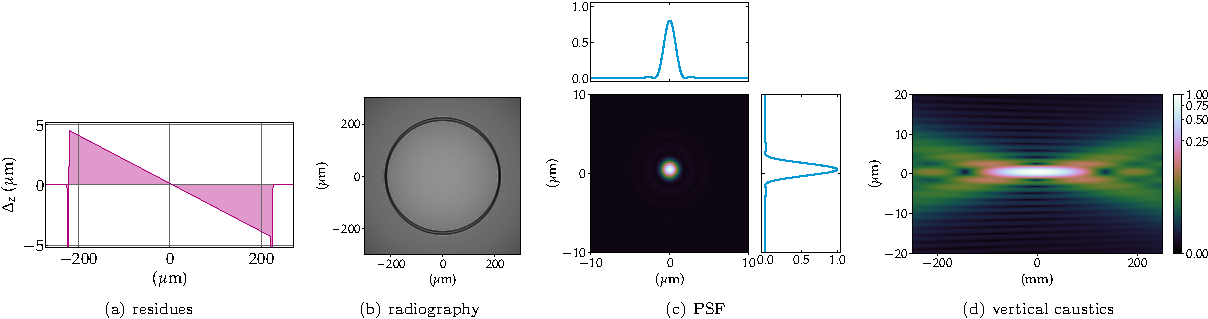
\includegraphics[height=4.19cm]{figures/ch04/offset_fs_CRL.pdf}
        \caption[Effects of the transverse offset of the parabolic section]{Simulations of a lens with front focusing parabolic section shifted by $\Delta_y=-2~\mu$m and back focusing shifted by $\Delta_y=-3~\mu$m - cf. Fig~\ref{fig:lens_cuts}(e). (a) Residual thickness, (b) phase-contrast image $150~$mm downstream the lens, (c) point spread function with cuts centred in $(0,0)$ and (c) the vertical beam caustics from $-250$~mm to $250$~mm in respect to the focal plane at $f=4.700~$m.} \label{fig:offset_fs_CRL}
\end{figure}

%-------------------------------------------------------------------------
%-------------------------------------------------------------------------
\subsubsection*{Tilted parabolic section}
%-------------------------------------------------------------------------
%-------------------------------------------------------------------------

When the axes of the parabolic front or/and back surfaces are not parallel to the optical axis, the lens active area appears to be tilted as shown in Figs.~\ref{fig:lens_cuts}(f)~and~(g). Similarly to what was introduced in the section \textit{Tilted lens} from \S\ref{sec:misalignments}~-~\textit{\nameref{sec:misalignments}}, both front and back surfaces are rotated according to the rotation matrices described in Eqs.~\ref{eq:affine} and the procedure described by Eq.~\ref{eq:affine2}. There are two subtle differences: the rotation angles from front and back surfaces can be chosen independently and rotation is only applied to the lens geometric aperture, and not to the whole front and back surfaces. The independent rotations allow for different regimes: one where both imprints are tilted with the same angle as in shown in Fig.~\ref{fig:lens_cuts}(f), which yields a residual phase similar to the one discussed in \textit{Tilted lens} from \S\ref{sec:misalignments}~-~\textit{\nameref{sec:misalignments}} and  one where there is no match of the front and back surfaces tilt, which yields an asymmetric residual phase as shown in Fig.~\ref{fig:tilt_fs_CRL}. By not applying the rotation to the region outside the lens geometric aperture, one avoids changing the lens projected thickness.

\begin{figure}[t]
        \centering
        {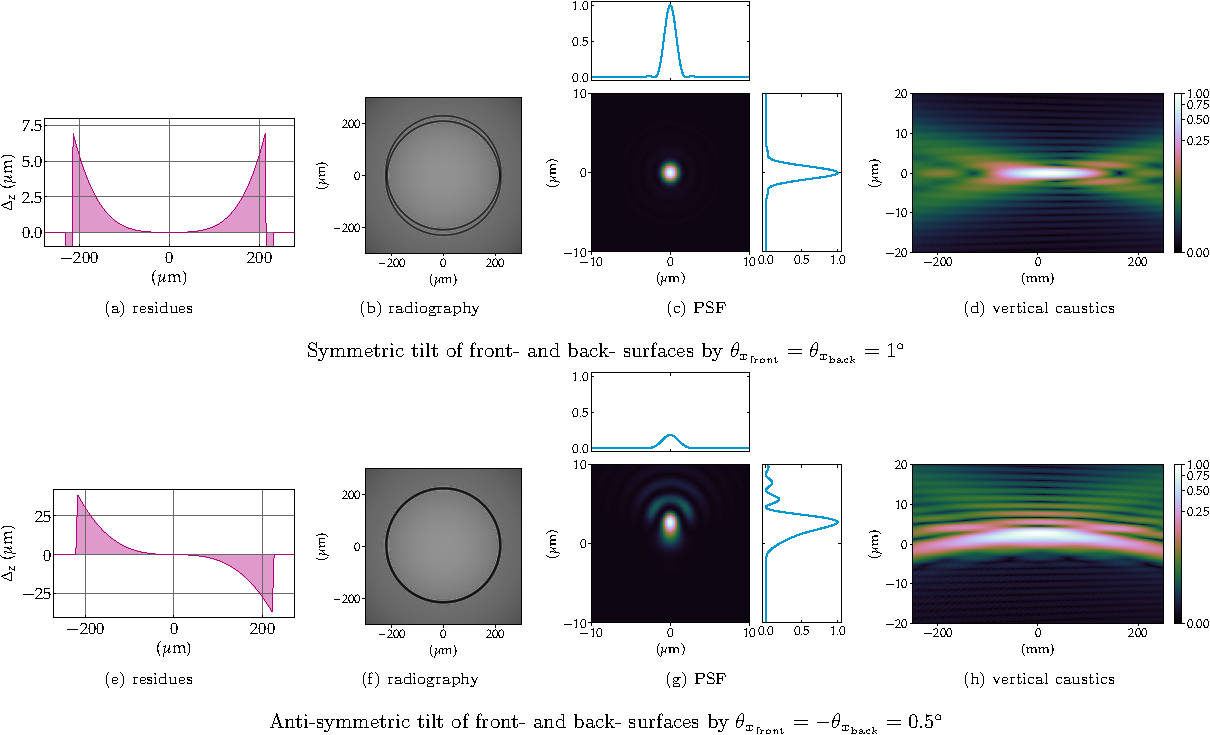
\includegraphics[width=1.\linewidth]{figures/ch04/tilt_fs_CRL.pdf}}
        \caption[Effects of the tilted parabolic section]{Simulations of a lens with front and back focusing parabolic sections independently tilted and shown in Fig~\ref{fig:lens_cuts}(f) and (g). The (a) residual thickness, (b) phase-contrast image $150~$mm downstream the lens, (c) point spread function with cuts centred in $(0,0)$ and (c) the vertical beam caustics from $-250$~mm to $250$~mm in respect to the focal plane at $f=4.700~$m of the symmetric tilt are shown on the top row. The (e) residual thickness, (f) phase-contrast image, (g) point spread function and (h) the vertical beam caustics for the anty-symmetric case with the same conditions is presented in the bottom row. While the symmetric case has a residual phase proportional to the 4$^{\text{th}}$ power of the lateral coordinates in the direction of the tilt, elongating the beam focusing in the propagation direction and shifting it on the same direction - typical of spherical aberrations, the residual phase of the anti-symmetric case has residual phase proportional to the 3$^{\text{rd}}$ power of the lateral coordinates in the direction of the tilt and has a PSF typical of coma-aberrated systems.  } \label{fig:tilt_fs_CRL}
\end{figure}

%-------------------------------------------------------------------------
%-------------------------------------------------------------------------
\subsection{Other sources of deviations from the parabolic shape}
%-------------------------------------------------------------------------
%-------------------------------------------------------------------------

So far, the modelling described here relies on translations and rotations of an ideal parabolic surface and investigating the residual phase. Another equally valid approach is to manipulate directly the residual phase and add it to the phase of an ideal focusing lens, which can be done fitting arbitrary surfaces or by introducing data from metrology of the optical element to be simulated.

\begin{figure}[t]
        \centering
        {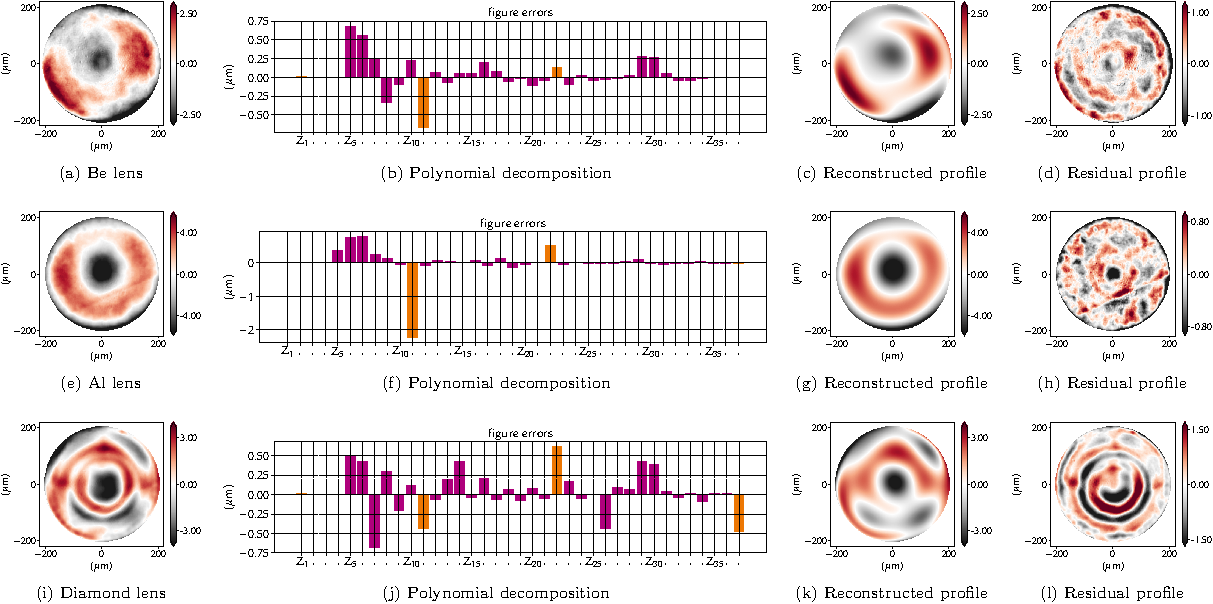
\includegraphics[width=1.\linewidth]{figures/ch04/metrology_zernike_profiles.pdf}}
        \caption[Other sources of deviations from the parabolic shape]{\textbf{First row}: (a) accumulated profile with RMS value: $\sigma_z=1.4~\mu$m, (b) Zernike circle polynomial decomposition of the profile in (a) and (c) the reconstruction based on the coefficients of a 2D-Beryllium lens with nominal radius $R\sim47.3~\mu\text{m}$ and useful aperture $A_{\diameter}\sim417~\mu\text{m}$ with RMS value: $\sigma_z=1.3~\mu$m. \textbf{Middle row}: (d) accumulated profile with RMS value: $\sigma_z=2.6~\mu$m, (e) Zernike circle polynomial decomposition of the profile in (d) and (f) the reconstruction based on the coefficients of a 2D-Aluminium lens with nominal radius $R\sim46.2~\mu\text{m}$ and useful aperture $A_{\diameter}\sim396~\mu\text{m}$ with RMS value: $\sigma_z=2.5~\mu$m. \textbf{Bottom row}: (g) accumulated profile with RMS value: $\sigma_z=1.8~\mu$m, (f) Zernike circle polynomial decomposition of the profile in (g) and (h) the reconstruction based on the coefficients of a 2D-diamond lens with nominal radius $R\sim103.4~\mu\text{m}$ and useful aperture $A_{\diameter}\sim402~\mu\text{m}$ with RMS value: $\sigma_z=1.6~\mu$m.}
        \label{fig:metrology_zernike_profiles}
\end{figure}

\begin{figure}[t]
        \centering
        {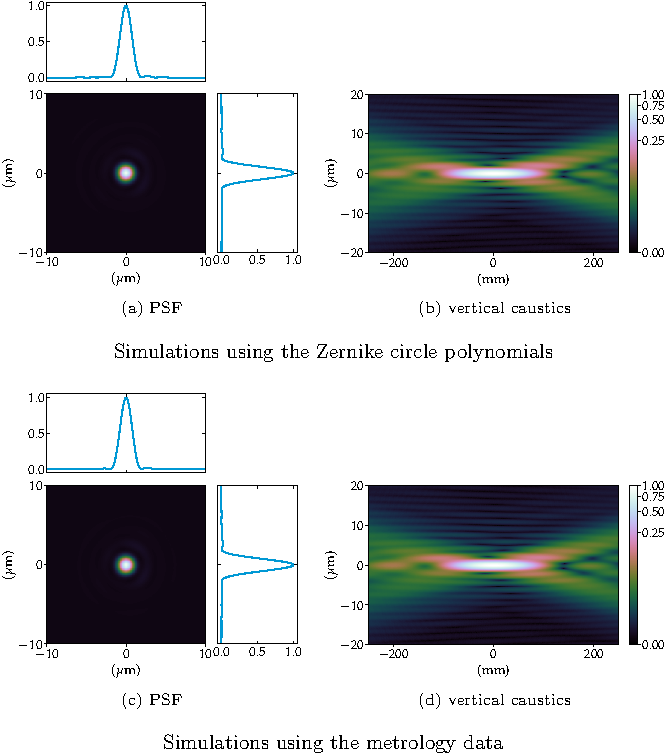
\includegraphics[height=11cm]{figures/ch04/metrology_zernike_simualtions.pdf}}
        \caption[Effects of other sources of deviations from the parabolic shape]{Simulations of a single 2D-Beryllium lens with nominal radius $R=50~\mu\text{m}$, geometric aperture $A_{\diameter}=440~\mu\text{m}$ and $t_\text{wall}=20~\mu$m at 8~keV. (a) and (c) point-spread function with cuts centred in $(0,0)$. (b) and (d) vertical beam caustics from -250~mm to 250~mm in respect to the focal plane. The difference between both profiles is almost not perceivable. This can be explained by the fact that the difference between the figure errors RMS value is almost negligible:  $\sigma_z=1.3~\mu$m (Zernike polynomial reconstruction) against $\sigma_z=1.4~\mu$m (metrology data), while the Mar\'echal criterion calculated for Beryllium lenses illuminated at $8$~keV requires the accumulated projected figure errors to be $\sigma_z\leq2.08~\mu$m, which makes the impact in the the reduction in intensity at the focal position is almost negligible - cf. Eqs.~\ref{eq:Strehl}-\ref{eq:ThickLim} for the Mar\'echal criteria and Strehl ratio in \textit{CRL performance: tolerance conditions for aberrations} from \S\ref{sec:refractive_optics}~-~\textit{\nameref{sec:refractive_optics}}.}\label{fig:metrology_zernike_simualtions}
\end{figure}

%-------------------------------------------------------------------------
%-------------------------------------------------------------------------
\subsubsection*{Orthornormal polynomials}
%-------------------------------------------------------------------------
%-------------------------------------------------------------------------

A widespread form of representing optical aberrations of arbitrary shapes is by decomposing them into an orthonormal base. Perhaps the most ubiquitous set of aberration functions is given by the Zernike polynomials for a circular aperture, first described in [\cite{Zernike1934}]. Their appeal comes from the fact that not only they are directly related to Seidel (primary), Schwarzschild (secondary) and tertiary-aberrations\footnote{This jargon comes from a power-series expansion of the aberration function. There are five primary aberrations, nine secondary aberrations and fourteen aberration terms for the tertiary aberrations. They all involve spherical aberration, coma, astigmatism, field
curvature, distortion and variations of thereof [\cite{Mahajan2013}].} but also include piston and tilts; they form an orthonormal base, which means that the value of the coefficients is not affected by the removal of a particular term [\cite{Mahajan2007}]. Another advantage of the Zernike polynomial decomposition is that each orthonormal aberration coefficient is the standard deviation for that particular aberration over the exit pupil, which is valuable when evaluating the optical system compliance with the  Mar\'echal criteria and calculating the Strehl ratio [\cite{Mahajan1983}].

For the aforementioned decomposition of the aberration function in an orthonormal base to retain its properties, the application of the circular Zernike polynomials must be limited to circular apertures. Other shapes of apertures with- or without obscuration can be obtained by Gram-Schmidt orthonormalisation and weighting of the Zernike circle polynomials [\cite{Swantner1994,Mahajan1995}]. X-ray optics systems often have a rectangular aperture and other two sets of polynomials are of particular interest in optical design: the set of orthonormal Zernike polynomials for a rectangular aperture  [\cite{Mahajan2007}] and the 2D-Legendre polynomial set for a rectangular aperture [\cite{Mahajan2010}]. Preferentially\footnote{Acknowledgments to Prof. V. Mahajan (University of Arizona, USA) and Prof. H. Gross (University of Jena, Germany) for the discussions on orthonormal polynomials in wavefront analysis and pointing out relevant literature.}, the Zernike circle polynomials are applied to 2D focusing lenses with a circular aperture. For 2D focusing X-ray lenses with square aperture, low aspect ratio between horizontal and vertical apertures and not strongly astigmatic focusing, e.g. crossed planar X-ray lenses, the Zernike rectangular polynomials are preferred. The 1D focusing lens is better fit by the 2D Legendre polynomial set\footnote{Please, refer to [\cite{Ye2014}] for a comparison between 2D orthonormal sets for square apertures.}. Analysing and describing refractive X-ray optics using circular Zernike and 2D Legendre polynomials were first presented by [\cite{Koch2016}]. Profiles generated by Zernike circle polynomials are shown in the right-hand side of Fig.~\ref{fig:metrology_zernike_profiles} and their effect on a coherent X-ray beam in Fig.~\ref{fig:metrology_zernike_simualtions}(a) and (b).

\newpage
%-------------------------------------------------------------------------
%-------------------------------------------------------------------------
\subsubsection*{Metrology data}
%-------------------------------------------------------------------------
%-------------------------------------------------------------------------

Any (unintentional) deviation of a parabolic shape can be considered as a source of manufacturing error. Each manufacturing process has some type of (signature) error associated to it and with the increasing number of exotic - or non-conventional - designs and tailored manufacturing strategies, it is beyond reasonable to create a model that could parametrise all sources of deviations from the parabolic shape. To circumvent that and to accurately model phase imperfection in compound refractive lenses, metrology data can also be used for optically imperfect X-ray lenses [\cite{Celestre2020, Chubar2020}]. Fig.~\ref{fig:metrology_zernike_profiles} shows three examples of lens figure errors from (a)-(c) a commercial pressed Beryllium lens, (d)-(f) an in-house pressed Aluminium lens and a (g)-(h) in-development laser-ablated Diamond lens from a commercial partner. The figure errors were measured with at-wavelength metrology and can be directly plugged into simulations as they describe the accumulated errors in projection approximation of both front and back focusing surfaces [\cite{Celestre2020, Berujon2020a, Berujon2020}]. The effect on a coherent X-ray of optical imperfections from metrology data is shown in Fig.~\ref{fig:metrology_zernike_simualtions}(c) and (d).

\begin{figure}[t]
        \centering
        {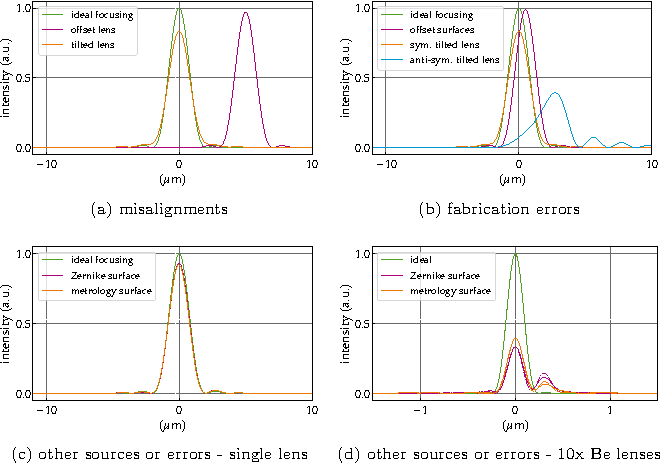
\includegraphics[width=1.\linewidth]{figures/ch04/Strehl}}
        \caption[Strehl ratio summarising the results from the diverse models presented]{Strehl ratio of the vertical cut at $x=0$ summarising the results from the diverse models presented.} \label{fig:Strehl}
\end{figure}

%-------------------------------------------------------------------------
%-------------------------------------------------------------------------
\subsection{Implementation}
%-------------------------------------------------------------------------
%-------------------------------------------------------------------------

The implementation of the modelling of the CRL, its misalignments and its figure errors is done using Python 3.7 and is fully compatible with the optical element class \texttt{SRWLOpt} described in the module \texttt{srwlib.py} from SRW\footnote{\url{github.com/ochubar/SRW}}. Each function representing either an X-ray lens or its figure errors returns a class \texttt{SRWLOptT} representing a generic transmission element storing amplitude transmission and optical path difference as a function of transverse coordinates. The main calculations for generating the X-ray lens transmission element is performed by the function \texttt{srwl\_opt\_setup\_CRL}. Apart from generating an ideal CRL (cf. Eq.~\ref{eq:TE_singlelens}), this function implements the degrees of freedom discussed in \S\ref{sec:misalignments}~-~\textit{\nameref{sec:misalignments}}; longitudinal and transverse offsets as well as the tilts of the individual parabolic sections as described in \S\ref{sec:fabrication}~-~\textit{\nameref{sec:fabrication}}. The generation of the residual phase errors based on the polynomial expansion of the aberration function in the exit pupil is done by \texttt{srwl\_opt\_setup\_CRL\_errors}. To calculate the aberration function, the user can either use a list with the polynomial coefficients or enter an RMS value for their sum (equivalent to fixing the piston value), in which case, they will be randomly calculated will comply with the RMS value limited by the user input. This function generates the residual errors and should be used in conjunction with \texttt{srwl\_opt\_setup\_CRL} to simulate an aberrated focusing lens. The aberration functions in \texttt{srwl\_opt\_setup\_CRL\_errors}\footnote{The functions used by \texttt{srwl\_opt\_setup\_CRL\_errors} to generate the 2D circular Zernike polynomials contain pieces of codes from the module \texttt{libtim-py} from Tim van Werkhoven, that had to be brought to Python 3.7 and in some places, small bugs fixed - this module has a Creative Commons Attribution-Share Alike
license. The 2D rectangular Zernike was originally inspired by the analytical formulation from the module \texttt{opticspy} from Xing Fan - this module has an MIT license. The formulation from the module was based on the equations from [\cite{Mahajan2007}], but had to be corrected with the errata published in [\cite{Mahajan2012}].} use the analytical solutions from [\cite{Mahajan2007}] with the corrections from [\cite{Mahajan2012}] and the solutions from [\cite{Mahajan2010}].  The generation of a surface based on the metrology data is done by \texttt{srwl\_opt\_setup\_CRL\_metrology}. The metrology data should be saved as an ASCII file (.dat) as defined by the function \texttt{srwl\_uti\_save\_intens\_ascii} from the module \texttt{srwlib.py}. The function \texttt{srwl\_opt\_setup\_CRL\_metrology} can be used to simulate figure errors, in which case, much like \texttt{srwl\_opt\_setup\_CRL\_errors} it requires the use of \texttt{srwl\_opt\_setup\_CRL} or it can be used to simulate a full measured profile. This library extension is currently available under a CC BY-SA 4.0 license at the \href{https://gitlab.esrf.fr/celestre/barc4RefractiveOptics}{barc4RefractiveOptics} GitLab repository\footnote{\url{gitlab.esrf.fr/celestre/barc4RefractiveOptics}}, where more information on the implemented functions can be found.

%-------------------------------------------------------------------------
%-------------------------------------------------------------------------
\section{Measuring optical imperfections in refractive lenses}
%-------------------------------------------------------------------------
%-------------------------------------------------------------------------

The metrology data shown in this section were taken on several beamtimes at the BM05 beamline - ESRF [\cite{Ziegler2004}] (from 2017 to 2018 - before the ESRF long shutdown for the EBS upgrade), at the 1-BM beamline - APS [\cite{Macrander2016}] (in 2019 during the ESRF long shutdown) and the ID06 beamline - ESRF [\cite{Kutsal_2019}] (in 2020 in the commissioning period of the ESRF-EBS upgrade)\footnote{Acknowledgements to Sébastien Bérujon and Ruxandra Cojocaru (BM05-ESRF); Xianbo Shi, Zhi Qiao, Michael Wojcik and Lahsen Assoufid (1-BM-APS-ANL); and to Carsten Detlefs (ID06-ESRF) for the help during the beamtimes.}.


%-------------------------------------------------------------------------
%-------------------------------------------------------------------------
\subsection{At wavelength-metrology}
%-------------------------------------------------------------------------
%-------------------------------------------------------------------------

%-------------------------------------------------------------------------
%-------------------------------------------------------------------------
\subsubsection*{X-ray speckle tracking}
%-------------------------------------------------------------------------
%-------------------------------------------------------------------------


%-------------------------------------------------------------------------
%-------------------------------------------------------------------------
\subsubsection*{Experimental setup}
%-------------------------------------------------------------------------
%-------------------------------------------------------------------------


[\cite{Berujon2020a, Berujon2020}]


%-------------------------------------------------------------------------
%-------------------------------------------------------------------------
\subsubsection*{Data processing and analysis}
%-------------------------------------------------------------------------
%-------------------------------------------------------------------------

%-------------------------------------------------------------------------
%-------------------------------------------------------------------------
\subsubsection*{Recommended literature}
%-------------------------------------------------------------------------
%-------------------------------------------------------------------------

At-wavelength-metrology, a niche-application of wavefront sensing, is a vast subject and it is out of scope to discuss in details all the most relevant literature available mainly due to its granularity. Current at-wavelength techniques used for evaluating the phase errors of CRLs (or individual X-ray lenses) are the Ronchigram [\cite{}], a technique based on ...; ptychography [\cite{}] ...; grating interferometry and all its variations [\cite{,,,,}] and speckle-tracking-based methods [\cite{,,,,}].

%-------------------------------------------------------------------------
%-------------------------------------------------------------------------
\subsection{Single lens measurements}
%-------------------------------------------------------------------------
%-------------------------------------------------------------------------

%-------------------------------------------------------------------------
%-------------------------------------------------------------------------
\subsection{Stacked lenses measurements}
%-------------------------------------------------------------------------
%-------------------------------------------------------------------------

%-------------------------------------------------------------------------
%-------------------------------------------------------------------------
\subsection{Corrective optics}
%-------------------------------------------------------------------------
%-------------------------------------------------------------------------

% %-------------------------------------------------------------------------
% %-------------------------------------------------------------------------
% \section{BARC4REFRACTIVE\_OPTICS}
% %-------------------------------------------------------------------------
% %-------------------------------------------------------------------------

$\blacksquare$
\addcontentsline{toc}{section}{References}
\printbibliography[heading=subbibliography]
\end{refsection}

 \cleardoublepage
\begin{refsection}
\chapter{Effect of optical imperfections on an X-ray beam}
\label{sec:effect_optical_imperfections}

The effects of the optical imperfections modelled and measured in Chapter~\ref{sec:measuring} to a X-ray beam are presented in this chapter in terms of fully- and partially- coherent simulations done with the \textit{SRW} code and the specially developed Python library for refractive optics (barc4RefractiveOptics) presented in Chapter~\ref{sec:modelling}. The fully-coherent simulations are composed of the beam-caustics and the point-spread function (PSF - intensity and phase) for the system being modelled. Partially-coherent simulations comprise the beam characteristics at the image plane and the beam profile at selected positions along the optical axis. These simulations are used to extensively evaluate the performance of commercially available Be lenses; compare the validity of individually measured and artificially stacked lenses against the stack measurement; and the different effects of distinct spatial frequency ranges in figure errors to the optical performance of the CRL.

%-------------------------------------------------------------------------
%-------------------------------------------------------------------------
\section{Lenses and lens stacks}\label{sec:lens_descripiton}
%-------------------------------------------------------------------------
%-------------------------------------------------------------------------
The modelled lenses are 2D-Be lenses with a nominal radius of $R=50~\mu\text{m}$ chosen as representative of lenses used widely at beamlines at many synchrotrons - see Fig.~\ref{fig:1D2D_lenses}(b) and (d). Such lenses have typically 1~mm thickness and are held in a 2\,mm thick lens frame (newer ones 1.6\,mm thick), which delimits the spacing $\Delta\text{s}=2~$mm between individual lenses in Eq.~\ref{eq:TE_CRL_MS_ERR}. Those lenses can be manufactured with wall thickness in the range of $\sim30~\text{to}~40~\mu\text{m}$. Applying Eq.~\ref{eq:A}, one obtains $A_{\diameter}\le440 \mu\text{m}$. At 8~keV, the energy used for the simulations, the index of refraction for Beryllium is $n=1-5.318\times10^{-6}+i\cdot2.071\times10^{-9}$ and the corresponding intensity transmission of this lenslet is shown in Fig.~\ref{fig:EffectiveAperure}(a). Applying Eq.~\ref{eq:CRL_classic} with $N=1$, one obtains the focal length for a single lens: $f_{\text{lens}}=4.701$~m. The lens stacks used are composed of $N=10$ lenses, except for the stacks used in the simulations shown in Fig.~\ref{fig:CDn01-05-10}, where the number of lenses $N$ varies ($N=1,5,10$).  The lens stack focal distance can be obtained by applying Eq.~\ref{eq:CRL} with $N=10$ and $L=(N-1)\cdot2~\text{mm}=18~\text{mm}$: $f_{\text{CRL}}=473~{\text{mm}}$, giving a magnification of approximately $126:1$ ($M\approx8\times10^{-3}$ for a source 60~m away from the CRL) and a diffraction-limited spot size (Eq.~\ref{eq:PSF}) of $\sim200~\text{nm}$. The error profiles used for the simulations have been described in \S\ref{sec:single_lens}~-~\textit{\nameref{sec:single_lens}} when measured individually and in \S\ref{sec:lens_stack}~-~\textit{\nameref{sec:lens_stack}} when measured as a 10-element stack.

The comparison between the simulations using individually measured lenses against simulations using metrology from a lens stack is shown in Fig.~\ref{fig:CDn_vs_CDnStack} for lenses L01-L10 and in Fig.~\ref{fig:CDo_vs_CDoStack} for the lenses L11-L20. Simulations of a single lens (L01), five stacked lenses (L01-L05) and ten stacked lenses (L01-L10) are used to investigate the deterioration of the X-ray beam profile upon stacking lenses. These can be seen in Fig.~\ref{fig:CDn01-05-10}. The effect of different spatial frequency ranges in the X-ray beam is shown in Fig.~\ref{fig:CDnFF_LF_HH}, where the performance of the accumulated figure error profile of lenses L01-L10 is compared against the performance of its decomposition in Zernike circular polynomials and the residues of such fit. Finally, the lens stack formed by individually measured lenses L01-L10 is meticulously studied under fully- and partially-coherent illumination. Figure~\ref{fig:CDnS} shows transverse cuts along the optical axis, the beam caustics, PSF (intensity and phase) and the demagnified image of the X-ray source (CPMU18\footnote{Cryogenic Permanent Magnet Undulator.}).

%-------------------------------------------------------------------------
%-------------------------------------------------------------------------
\section{Software and computing infrastructure}\label{sec:SRW}
%-------------------------------------------------------------------------
%-------------------------------------------------------------------------

All simulations presented here were done using the "Synchrotron Radiation Workshop" (SRW) [\cite{Chubar1998}]\footnote{Available at \url{https://github.com/ochubar/srw}}, as it conveniently offers the possibility of fully- and partially-coherent calculations\footnote{See \S\ref{sec:wave_propag}~-~\textit{\nameref{sec:wave_propag}} and \S\ref{sec:partially_coherent}~-~\textit{\nameref{sec:partially_coherent}}.}, and presents native parallelisation with the MPI standard [\cite{Chubar2011}]. Fully coherent calculations were done using a single CPU of an Intel(R) Xeon(R) CPU E5-2680 v4 @ 2.40GHz, while partial coherent simulations used 28 CPUs of the same computer infrastructure (NICE OAR cluster at the ESRF). The specially developed python library for dealing with the refractive lenses with the addition of optical imperfections (barc4RefractiveOptics) presented in Chapter~\ref{sec:modelling} was also used in the simulations.

\begin{figure}[t]
        \centering
        {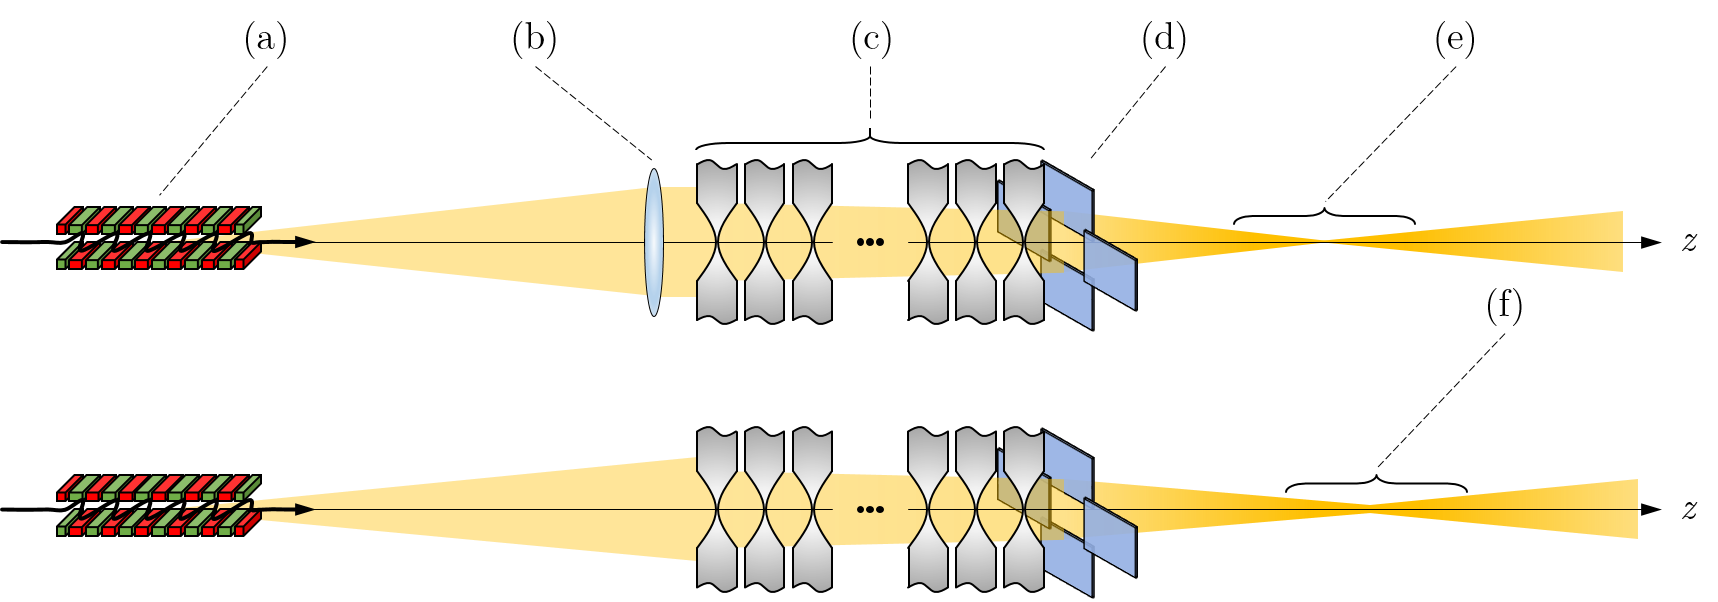
\includegraphics[width=0.8\linewidth]{figures/ch05/optical_setups.png}}
        \caption[Beamlines for coherent- and partially-coherent simulations]{\textbf{top row}: beamealine used for  \S\ref{sec:coherent_sim}~-~\textit{\nameref{sec:coherent_sim}}. \textbf{bottom row}: beamealine used for  \S\ref{sec:partcoherent_sim}~-~\textit{\nameref{sec:partcoherent_sim}}. (a) shows the X-ray source: a CPMU18 undulator. An (b) ideal parabolic phase element with radius of curvature $R=-60~$m is placed 60~m downstream the radiation source to give the illumination a near-plane phase - cf. Eq.~\ref{eq:planewave}. This ideal element is only present for the fully-coherent simulations. The lenses being studied are shown in (c). They are immediately followed by a set of (d) slits to ensure the same geometric aperture for all simulations and aid direct calculation of the Strehl ratio. For the fully-coherent simulations, the beam-caustic range is shown in (e) and the PSF is calculated at the centre of it. For the partially-coherent simulations, the beam profile evolution along the optical axis is shown in (f) and the beam characteristics at the focal position are calculated at the its centre. 
        }\label{fig:optical_setups}
\end{figure}

%-------------------------------------------------------------------------
%-------------------------------------------------------------------------
\section{Fully coherent simulations}\label{sec:coherent_sim}
%-------------------------------------------------------------------------
%-------------------------------------------------------------------------

For this set of simulations, the X-ray source is a filament electron-beam passing through a CPMU18 undulator with 111 magnetic periods, $\Lambda=18$~mm magnetic period and magnetic field $B=0.9863~$T emitting a 1$^\text{st}$ harmonic photon beam at 8~keV (resonance). The photon source size and divergence are given by the specific radiation
pattern size and divergence of the insertion device and the emission is fully coherent\footnote{cf. \S\ref{sec:optical_coherence}~-~\textit{\nameref{sec:optical_coherence}}.}  - see \S\ref{sec:brilliance}~-~\textit{\nameref{sec:brilliance}}. At 60~m away from the source, the beam footprint\footnote{Although commonly approximated by Gaussian distributions, undulator emission does not posses Guassian distribution not even at resonance. Please, refer to footnote \ref{note:und_prof} in \S\ref{sec:brilliance}~-~\textit{\nameref{sec:brilliance}} for a deeper discussion on the emission profile of undulator radiation and for further references.} is large enough to illuminate the full geometric aperture of a lens with $A_{\diameter}\le440 \mu\text{m}$ with an intensity variation of 2\% (centre to the edge). The illumination profile in conjunction with the transmission profile of the lenses being modelled (Fig.~\ref{fig:EffectiveAperure}) allows to classify such systems as apodised. In the paraxial approximation, the radiation phase for this source is dominated by a quadratic phase term [\cite{Chubar1999, Chubar2001b, Chubar2019}]. At the position along the optical axis where the intensity is calculated, this quadratic phase term can be compensated by placing an ideal lens with focal length focal length $f=-60~$m. This ensures a plane-wave illumination (Eq.~\ref{eq:planewave}) downstream the ideal element, which is used to illuminate the different CRL models being studied. The lens stack and imperfect lenses are modelled using the CRL multi-slice approach with errors added described by Eq.~\ref{eq:TE_CRL_MS_ERR} and shown in Fig.~\ref{fig:models}(c) in \S\ref{sec:CRL_modelling}~-~\textit{\nameref{sec:CRL_modelling}}. The evaluation of the effect of optical imperfections on an X-ray beam is performed at the image plane of the focusing system and on its vicinity. The beamline used for the fully-coherent simulations is shown in  Fig.~\ref{fig:optical_setups}.



\begin{table}[h]
\caption[FWHM of the PSF for the simulated models in Figs.~\ref{fig:CDn_vs_CDnStack}-\ref{fig:CDnS}]{Summary of the beam sizes in FWHM for various CRL models. The extended source image sizes are taken from the partially coherent simulations averaging the intensity of 10$^{4}$ wavefronts.}\label{tab:beamsizes}\small

\centering
\begin{tabular}{lrcccc}\hline \hline
&                        &\multicolumn{2}{c}{\textbf{PSF} (nm)}   &\multicolumn{2}{c}{\textbf{source image} (nm)}\\
&\textbf{lens model}     &hor.           &ver.                    &hor.            &ver. \\ \cline{2-6}
&analytic equations       &\multicolumn{2}{c}{223.3}           &603.8           &241.7 \\
&ideal CRL               &217.5          &218.7                   &626.4           &247.5 \\ \hline
Fig.~\ref{fig:CDn_vs_CDnStack} &L01-L10  &208.8  &210.1           &680.1           &254.4 \\
&stack 01                &206.2          &219.5                   &692.0           &254.1\\ \hline
Fig.~\ref{fig:CDo_vs_CDoStack} &L11-L20  &194.7  &197.5           &835.1           &374.8 \\
&stack 02                &192.1          &203.1                   &748.6           &268.9 \\ \hline
Fig.~\ref{fig:CDn01-05-10}&single ideal lens  &\multicolumn{2}{c}{1959.4}   & -    & -\\
&L01                     &1954.0         &1957.3                  & -              & - \\
&five ideal stacked lenses  &\multicolumn{2}{c}{401.3}            & -              & - \\
&L01-L05                 &384.5       &399.0                      & -              & - \\ \hline
Fig.~\ref{fig:CDnFF_LF_HH} &LF L01-L10  &214.8     &206.0         & 731.4          &263.7 \\
&HF L01-L10              &225.1      &231.6                       & 637.5          &246.1 \\
\hline \hline
\end{tabular}
\end{table}{}


%-------------------------------------------------------------------------
%-------------------------------------------------------------------------
\subsection{The PSF: ideal focusing}\label{sec:psf_sim}
%-------------------------------------------------------------------------
%-------------------------------------------------------------------------

After passage through the CRL model being studied, the plane wave used for illuminating the optical system will develop a quadratic phase term that has a curvature radius equivalent to the effective focal distance of the optical system, which is given by Eq.~\ref{eq:CRL}. The propagation of the wavefront from the exit pupil of the CRL to the image plane located a focal length distance is equivalent to an optical 2D-Fourier transform of the system pupil function. The PSF of the optical system corresponds to the squared modulus of this Fourier transform, which is the wavefront intensity at the focal plane, considering a plane wave illumination [\cite[\textit{\S2.3.1} \& \textit{\S6.2}]{Goodman2017}]. The phase of the propagated field at the focal position, the normalised PSF and relative intensities of the aberrated PSF normalised to the ideal case (Strehl ratio) are shown in Figs.~\ref{fig:CDn_vs_CDnStack}-\ref{fig:CDo_vs_CDoStack}(b-c) and (e);  Fig.~\ref{fig:CDn01-05-10}(b)-(d); Fig.~\ref{fig:CDnFF_LF_HH}(b-c) and (e); and Fig.~\ref{fig:CDnS}(d)-(e). The calculated FWHM of the central lobe of the PSF for the simulated models presented in Figs.~\ref{fig:CDn_vs_CDnStack}-\ref{fig:CDnS} are displayed on Table~\ref{tab:beamsizes} and the respective Strehl ratio, compiled in Table~\ref{tab:Strehl}.


\begin{table}[t]
\caption[Strehl ratio for the simulated models in Figs.~\ref{fig:CDn_vs_CDnStack}-\ref{fig:CDnS}]{Comparison of the Strehl ratio for the simulated models in Figs.~\ref{fig:CDn_vs_CDnStack}-\ref{fig:CDnS}}\label{tab:Strehl}%\small
\resizebox{\columnwidth}{!}{
\centering
\begin{tabular}{lrcccccc}\hline \hline
&\textbf{lens model}     &$\sigma_z$ ($\mu$m)     &$S_{\text{a}}$ (Eq.~\ref{eq:Strehl})  &$S_{\text{b}}$  (Eq.~\ref{eq:Marechal}) &$S_{\text{c}}$  (Eq.~\ref{eq:Mahajan}) &Coherent &Partially-coherent \\ \cline{2-8}
Fig.~\ref{fig:CDn_vs_CDnStack} &L01-L10  &4.84  &0.067      &0.285 &0.393  &0.394          &0.409 \\
&stack 01                                &5.75  &-          &0.054 &0.215  &0.374          &0.375\\ \hline
Fig.~\ref{fig:CDo_vs_CDoStack} &L11-L20  &6.28  &-          &0.007 &0.160  &0.185          &0.211 \\
&stack 02                                &6.48  &-          &0.001 &0.142  &0.243          &0.247 \\ \hline
Fig.~\ref{fig:CDn01-05-10} &L01          &0.57  &0.985      &0.985 &0.985  &0.981          & -  \\
&L01-L05                                 &2.67  &0.669      &0.696 &0.718  &0.684          & - \\ \hline
Fig.~\ref{fig:CDnFF_LF_HH} &LF L01-L10   &4.36  &0.116      &0.311 &0.413  &0.335          &0.359 \\
&HF L01-L10                              &2.18  &0.779      &0.791 &0.802  &0.796          &0.778 \\
\hline \hline
\end{tabular}
}
\end{table}{}


%-------------------------------------------------------------------------
%-------------------------------------------------------------------------
\subsection{The beam caustics}\label{sec:caustics_sim}
%-------------------------------------------------------------------------
%-------------------------------------------------------------------------

The beam characteristics at the image plane are very important and the PSF simulations in Figs.~\ref{fig:CDn_vs_CDnStack}~to~\ref{fig:CDnS} show obvious differences between ideal and aberrated focusing of CRLs. It is necessary, however, to complement this with investigations of the effect of optical imperfections away from the focal position, especially because several experimental applications may use a defocused beam. To get an overview of the beam evolution up- and downstream the focal position, one can propagate the wavefront along the optical axis and for each position extract a cross-section of the beam. This will be referred to as the beam caustic\footnote{Strictly speaking, the beam caustic is the envelope of light rays after passing through an optical element - see p.~60 [\cite{Lawrence1972}]. A more comprehensive theory of caustics in optics is given by [\cite{Kravstov1999, Nye1999}].}. The beam caustics are shown in Figs.~\ref{fig:CDn_vs_CDnStack}-\ref{fig:CDnFF_LF_HH}(a); and Fig.~\ref{fig:CDnS}(c). The beam cross-section for selected positions along the beam optical axis can be seen in Fig.~\ref{fig:CDnS}(b). The vertical cuts were taken at $x=0$. The zero position along the optical axis is given by the distance from the centre of the CRL to the image plane, position where the PSF is calculated. To calculate the beam caustics, the wavefront was propagated from 10~mm upstream the focal position to 10~mm downstream in 4001 equally spaced steps along the optical axis.

%-------------------------------------------------------------------------
%-------------------------------------------------------------------------
\section{Partially coherent simulations}\label{sec:partcoherent_sim}
%-------------------------------------------------------------------------
%-------------------------------------------------------------------------

The PSF and beam caustic simulations presented previously are both fully-coherent calculations. They present the focusing of a perfect plane wavefront to a diffraction-limited spot. This shows the intrinsic limitations of the optical system, but inherently neglects the effects of an extended and partially coherent source.

%-------------------------------------------------------------------------
%-------------------------------------------------------------------------
\subsection{X-ray source}\label{sec:source_sim}
%-------------------------------------------------------------------------
%-------------------------------------------------------------------------
The emission of a single electron passing through an undulator (filament beam) is fully coherent. By changing the electron initial conditions (positions, direction and energy), propagating the emission of this electron through the beamline and adding up intensities, one can simulate partially coherent radiation if the electron beam phase space (5D) is sufficiently sampled as discussed in \S\ref{sec:partially_coherent}~-~\textit{\nameref{sec:partially_coherent}} - see also [\cite{Chubar2011}]. 

For this section, a hypothetical beamline operating on the new Extremely Brilliant Source (ESRF-EBS) magnetic lattice [\cite{orangebook}] is implemented. This beamline is shown in Fig.\ref{fig:optical_setups}. The beamline sits on a straight section and has a CPMU18 undulator as an insertion device. The undulator was tuned to its first harmonic at 8~keV for all simulations. The photon source size is $\sim71.92\times12.38~\mu\text{m}^2$ and its divergence $\sim17.66\times14.72~\mu\text{rad}^2$ (FWHM, horizontal vs. vertical). The first optical element was placed 60~m downstream of the centre of the undulator to ensure a beam footprint larger than the geometric aperture of the CRL being studied ($A_{\diameter}\sim440~\mu\text{m}$) and a constant intensity over it. The transverse coherence length $\Delta_{\textbf{cl}_{\perp}}$ at the entrance of the optical system is estimated to be $\sim60\times448~\mu\text{m}^2$ (FWHM, horizontal vs. vertical), from the calculation of the complex degree of spatial coherence\footnote{see \textit{Spatial coherence} in \S\ref{sec:optical_coherence}~-~\textit{\nameref{sec:optical_coherence}}.} $j(\textbf{r}_1,\textbf{r}_2)$ - see Fig.~\ref{fig:CDoC}. If there is no spatial filtering, the horizontal direction is less coherent than in the vertical, leading to stronger blurring of the image in the less coherent direction [\cite[\textit{\S7.5}]{Goodman2017}]. 

\begin{figure}[t]
        \centering
        {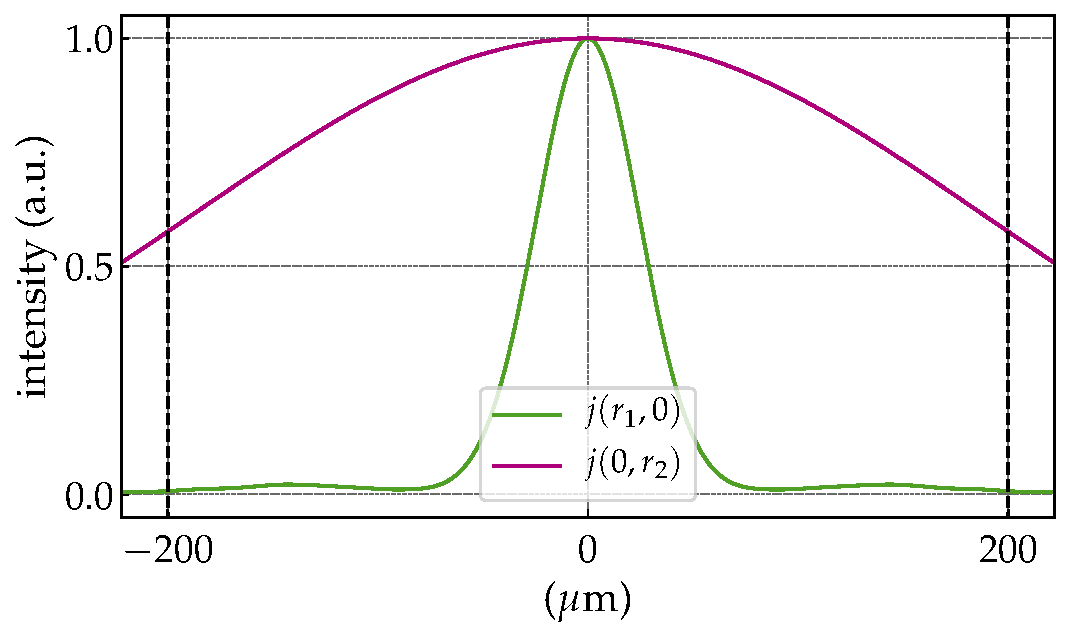
\includegraphics[height=4cm]{figures/ch05/source/CdoC.pdf}}
        \caption[Complex degree of coherence]{Horizontal ($j(\textbf{r}_1,0)$) and vertical ($j(0,\textbf{r}_2)$) cuts of the complex degree of coherence function immediately before the CRL - see \S\ref{sec:source_sim}~-~\textit{\nameref{sec:source_sim}}. The vertical dashed lines indicate the geometric aperture used for the simulations. 
        }\label{fig:CDoC}
\end{figure}
%-------------------------------------------------------------------------
%-------------------------------------------------------------------------
\subsubsection*{On the convergence of the simulations}
%-------------------------------------------------------------------------
%-------------------------------------------------------------------------
In a conservative approach, the partially coherent simulations presented here were done using 10$^{4}$ wavefronts to ensure convergence.
The convergence of the partially-coherent simulations is connected to the sampling of the electron distribution $f(s,s',\gamma_e)$, where each electron in a bunch has a different initial condition in terms of position $s=(x_e,y_e,z_e=0)$, direction $s'=(x'_e,y'_e)$ and energy $\gamma_e$ - see \textit{Physical-optics-based methods} in \S\ref{sec:partially_coherent}~-~\textit{\nameref{sec:partially_coherent}}. \todo{Fig.~\ref{fig:ME_convergence} shows the sampling of the function $f(s,s',\gamma_e)$ for the ESRF-EBS, the old ESRF-low $\beta$ and the old ESRF-high $\beta$ straight sections.}

\begin{table}[t]
\caption[Electron-beam parameters for the ESRF-ESB, the old ESRF-low $\beta$ and the old ESRF-high $\beta$ straight sections]{\todo{Electron-beam parameters for the ESRF-ESB, the old ESRF-low $\beta$ and the old ESRF-high $\beta$ straight sections.}}\label{tab:E_beam_param}
\centering
\begin{tabular}{rccc}

\end{tabular}
\end{table}{}

%-------------------------------------------------------------------------
%-------------------------------------------------------------------------
\subsection{Beam characteristics at the focal position}\label{sec:source_image_sim}
%-------------------------------------------------------------------------
%-------------------------------------------------------------------------

The image of the extended X-ray source is similar to the convolution between the geometrically demagnified image of the source and the 2D-PSF of the imaging system, provided the beam is not strongly cropped anywhere in the beamline being simulated. For the cases being studied here, the beam footprint at the entrance pupil of the CRL system is several times larger than the geometric aperture of a single lens and this convolution approach is not valid, hence the necessity of the partially-coherent simulations for imaging the centre of the CPMU18. Figures~\ref{fig:CDn_vs_CDnStack}-\ref{fig:CDo_vs_CDoStack}(e), Fig.~\ref{fig:CDnFF_LF_HH}(e) and Fig.~\ref{fig:CDnS}(f) show the normalised demagnified image of the undulator photon source while Table~\ref{tab:beamsizes} presents the horizontal and vertical FWHM for those simulations. Figures~\ref{fig:CDn_vs_CDnStack}-\ref{fig:CDo_vs_CDoStack}(f) and Fig.~\ref{fig:CDnFF_LF_HH}(f) show graphical representation of the Strehl irradiance ratio, as the intensities of the aberrated models are normalised to the peak intensity of the aberration-free CRL model. These values are compiled in Table~\ref{tab:Strehl}.

%-------------------------------------------------------------------------
%-------------------------------------------------------------------------
\subsection{Beam profile evolution along the optical axis}\label{sec:partcaustics_sim}
%-------------------------------------------------------------------------
%-------------------------------------------------------------------------

Calculating the full beam caustic with partially-coherent simulations is impractical using current simulation methods and computers/clusters especially if: \textit{i}-)  the beamline does not present a very high degree of coherence, thus requiring a very large number of wavefronts to accurately simulate the partial-coherence; \textit{ii}-) the beamline has low transmission (strong beam cropping, diffraction orders outside apertures); or \textit{iii}-) the sampling along the optical axis is high. Still, many applications require to operate up- or downstream of the focal position and assessing the beam quality on such positions is essential. Figure~\ref{fig:CDnS}(a) shows the beam profile evolution spanning 20~mm along the optical axis for selected positions up- and downstream the image plane. Images are displayed showing their relative intensity to the beam in the focal plane. The positions chosen were the same as in Fig.~\ref{fig:CDnS}(b), selected cuts along the beam caustics, so direct comparison between fully- and partially-coherent simulations can be done.

\clearpage

\begin{figure}[t]
        \centering
        {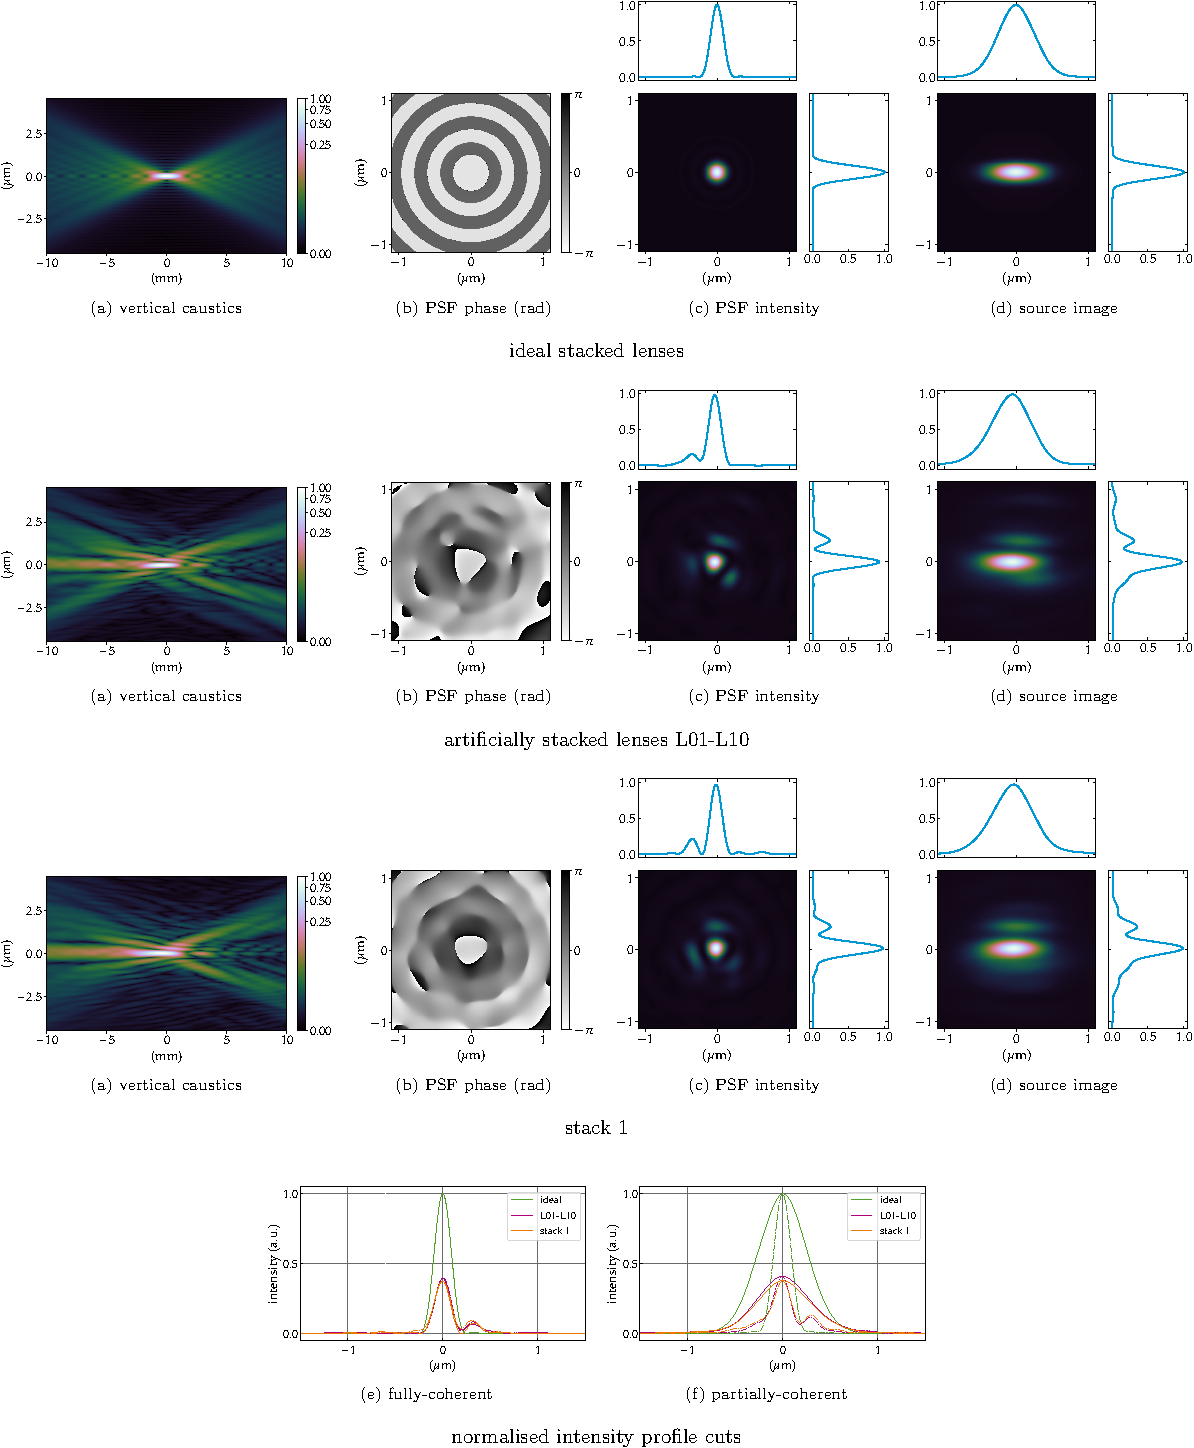
\includegraphics[width=1\linewidth]{figures/ch05/CDn_vs_CDnStack.pdf}}
        \caption[Artificially stacked lenses L01-L11 vs. stack 1 comparison]{Comparison between individually-measured lenses L01-L10 against the stack metrology of the same lenses. \textbf{top row}: ideal CRL, \textbf{upper middle row}: L01-L10 artificially stacked lenses measured individually. \textbf{lower middle row}: lenses measured as a stack. \textbf{bottom row}: ($-$) horizontal and (-~-) vertical intensity cuts (Strehl ratio) for coherent- and partially-coherent simulations. The simulated CRLs are composed of 10 2D-Beryllium lens with nominal radius $R=50~\mu\text{m}$, geometric aperture $A_{\diameter}=440~\mu\text{m}$ and $t_\text{wall}=20~\mu$m at 8~keV. The error profiles used are shown in Fig.~\ref{fig:accumulated_profile_1} and \ref{fig:CDn}.}\label{fig:CDn_vs_CDnStack}
\end{figure}

\begin{figure}[t]
        \centering
        {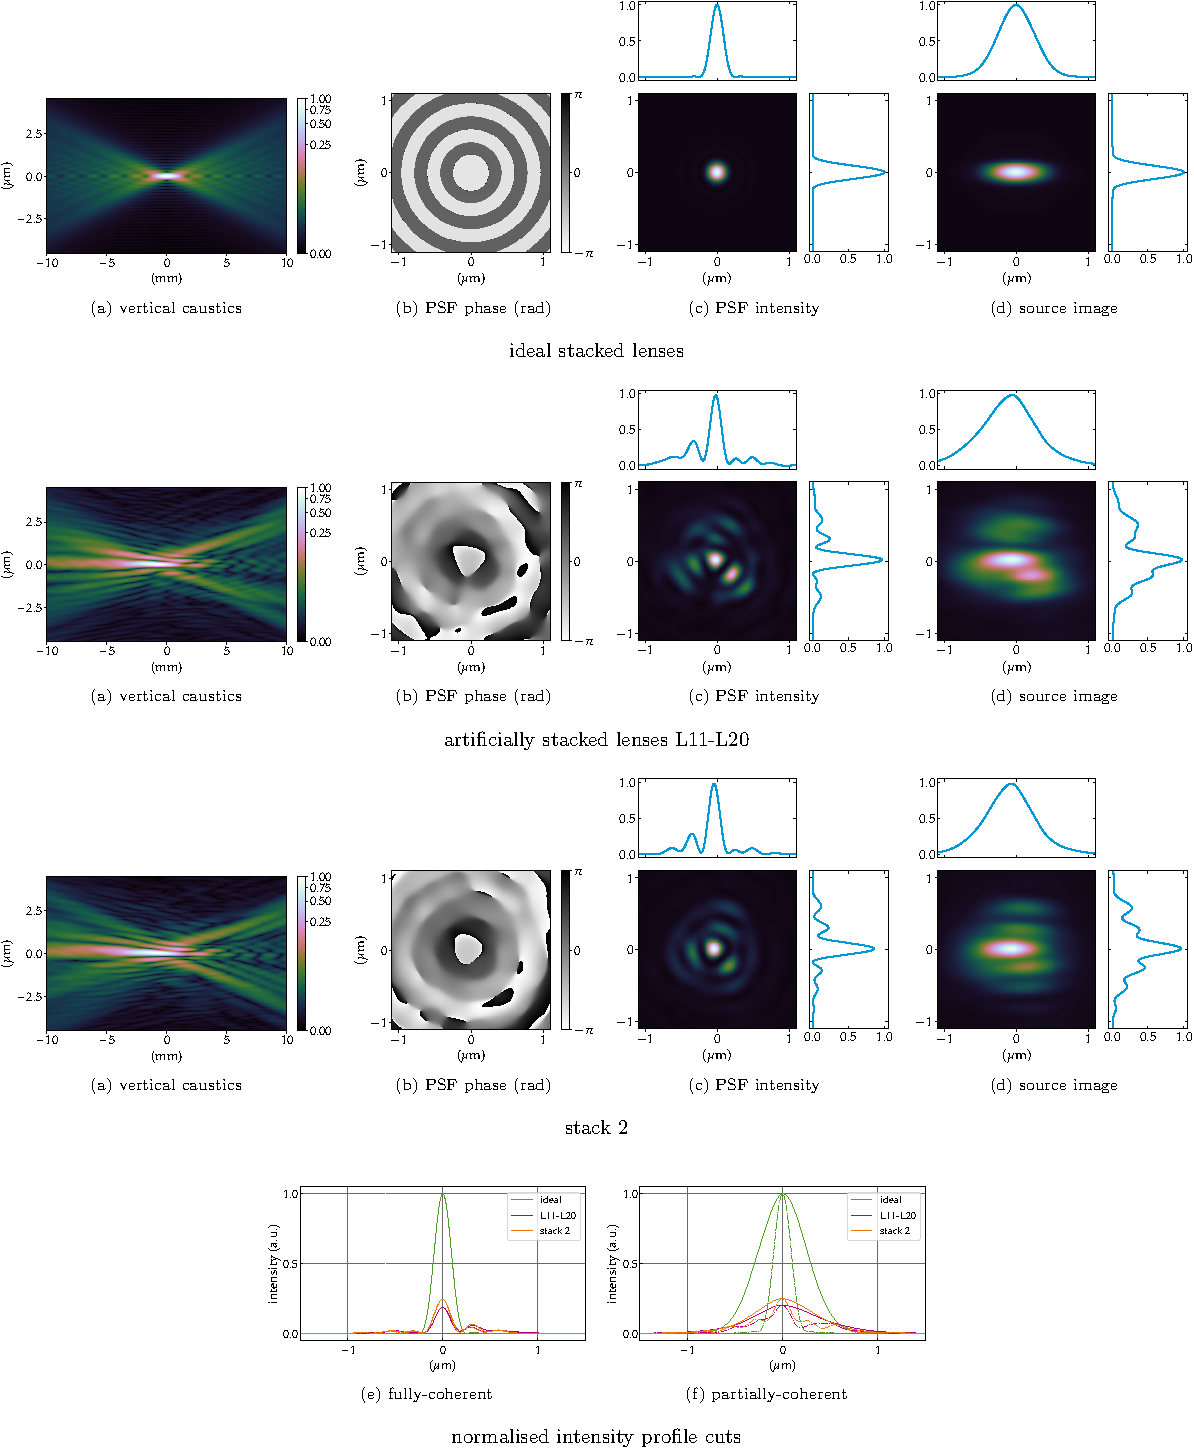
\includegraphics[width=1\linewidth]{figures/ch05/CDo_vs_CDoStack.pdf}}
        \caption[Artificially stacked lenses L11-L21 vs. stack 2 comparison]{Comparison between individually-measured lenses L11-L20 against the stack metrology of the same lenses. \textbf{top row}: ideal CRL, \textbf{upper middle row}: L11-L20 artificially stacked lenses measured individually. \textbf{lower middle row}: lenses measured as a stack. \textbf{bottom row}:($-$) horizontal and (-~-) vertical intensity cuts (Strehl ratio) for coherent- and partially-coherent simulations. The simulated CRLs are composed of 10 2D-Beryllium lens with nominal radius $R=50~\mu\text{m}$, geometric aperture $A_{\diameter}=440~\mu\text{m}$ and $t_\text{wall}=20~\mu$m at 8~keV. The error profiles used are shown in Fig.~\ref{fig:accumulated_profile_2} and \ref{fig:CDo}.}\label{fig:CDo_vs_CDoStack}
\end{figure}

\begin{figure}[t]
        \centering
        {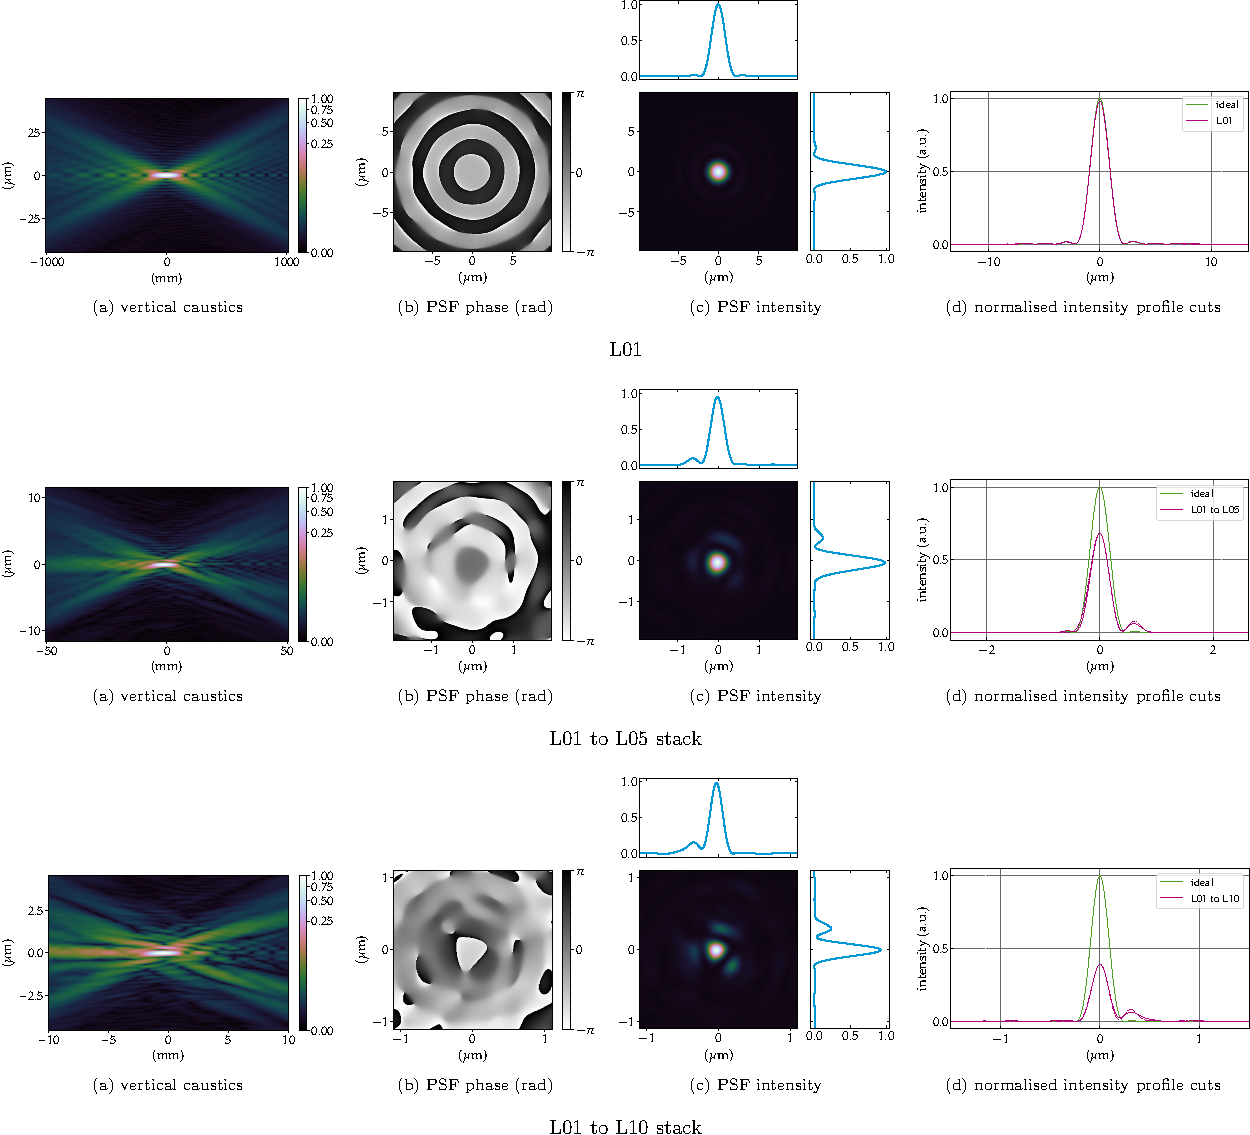
\includegraphics[width=1\linewidth]{figures/ch05/CDn01-05-10.pdf}}
        \caption[Effects of stacking lenses]{Effects of artificially stacking individually measured lenses. \textbf{top row}: single L01 lens performance). \textbf{lower middle row}: L01-L05 artificially stacked lenses. \textbf{bottom row} L01-L10 artificially stacked lenses. The simulated CRLs are composed of 2D-Beryllium lens with nominal radius $R=50~\mu\text{m}$, geometric aperture $A_{\diameter}=440~\mu\text{m}$ and $t_\text{wall}=20~\mu$m at 8~keV.}\label{fig:CDn01-05-10}
\end{figure}

\begin{figure}[t]
        \centering
        {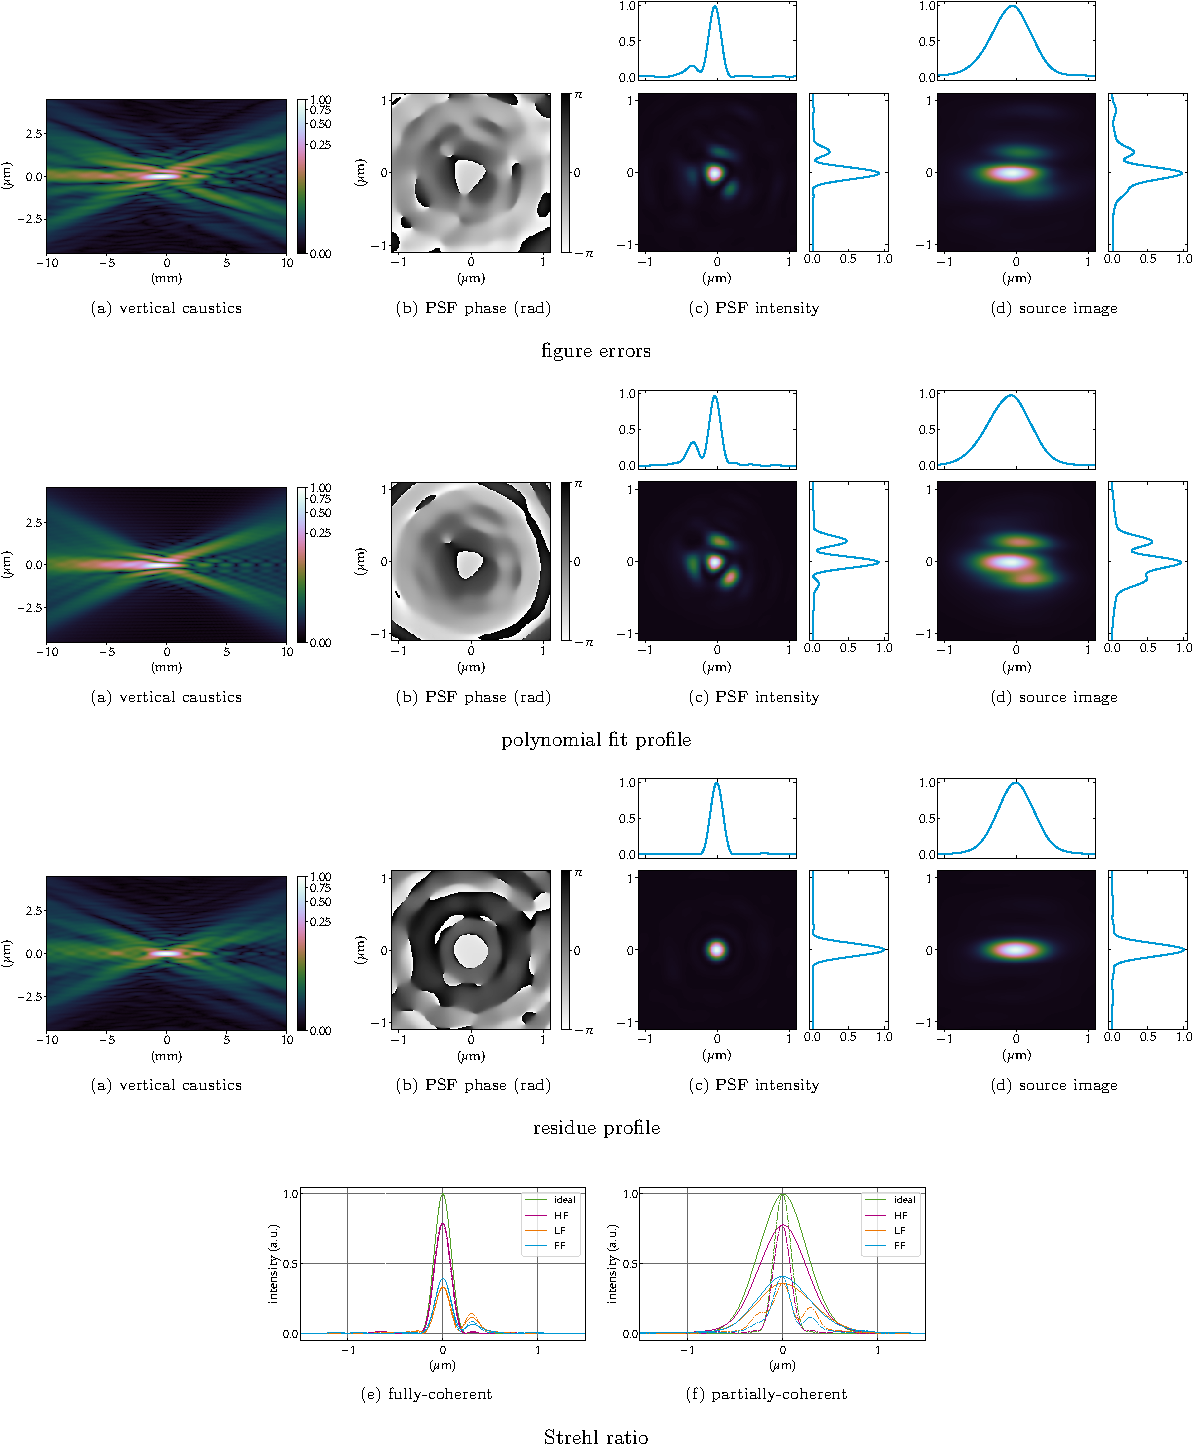
\includegraphics[width=1\linewidth]{figures/ch05/CDnFF_LF_HH.pdf}}
        \caption[Effects of different spatial frequencies ranges on a X-ray beam]{Effects of different spatial frequencies ranges on a X-ray beam. \textbf{top row}: full accumulated profile of individually measured and artificially measured L01-L10 lenses. \textbf{upper middle row}: Zernike circle polynomial reconstruction of the accumulated profile. \textbf{lower middle row}: residual profile from the fit. \textbf{bottom row}:($-$) horizontal and (-~-) vertical intensity cuts (Strehl ratio) for coherent- and partially-coherent simulations. The simulated CRLs are composed of 10 2D-Beryllium lens with nominal radius $R=50~\mu\text{m}$, geometric aperture $A_{\diameter}=440~\mu\text{m}$ and $t_\text{wall}=20~\mu$m at 8~keV. The error profiles used are shown in Fig.~\ref{fig:accumulated_profile_1}.}\label{fig:CDnFF_LF_HH}
\end{figure}

\begin{figure}[t]
        \centering
        {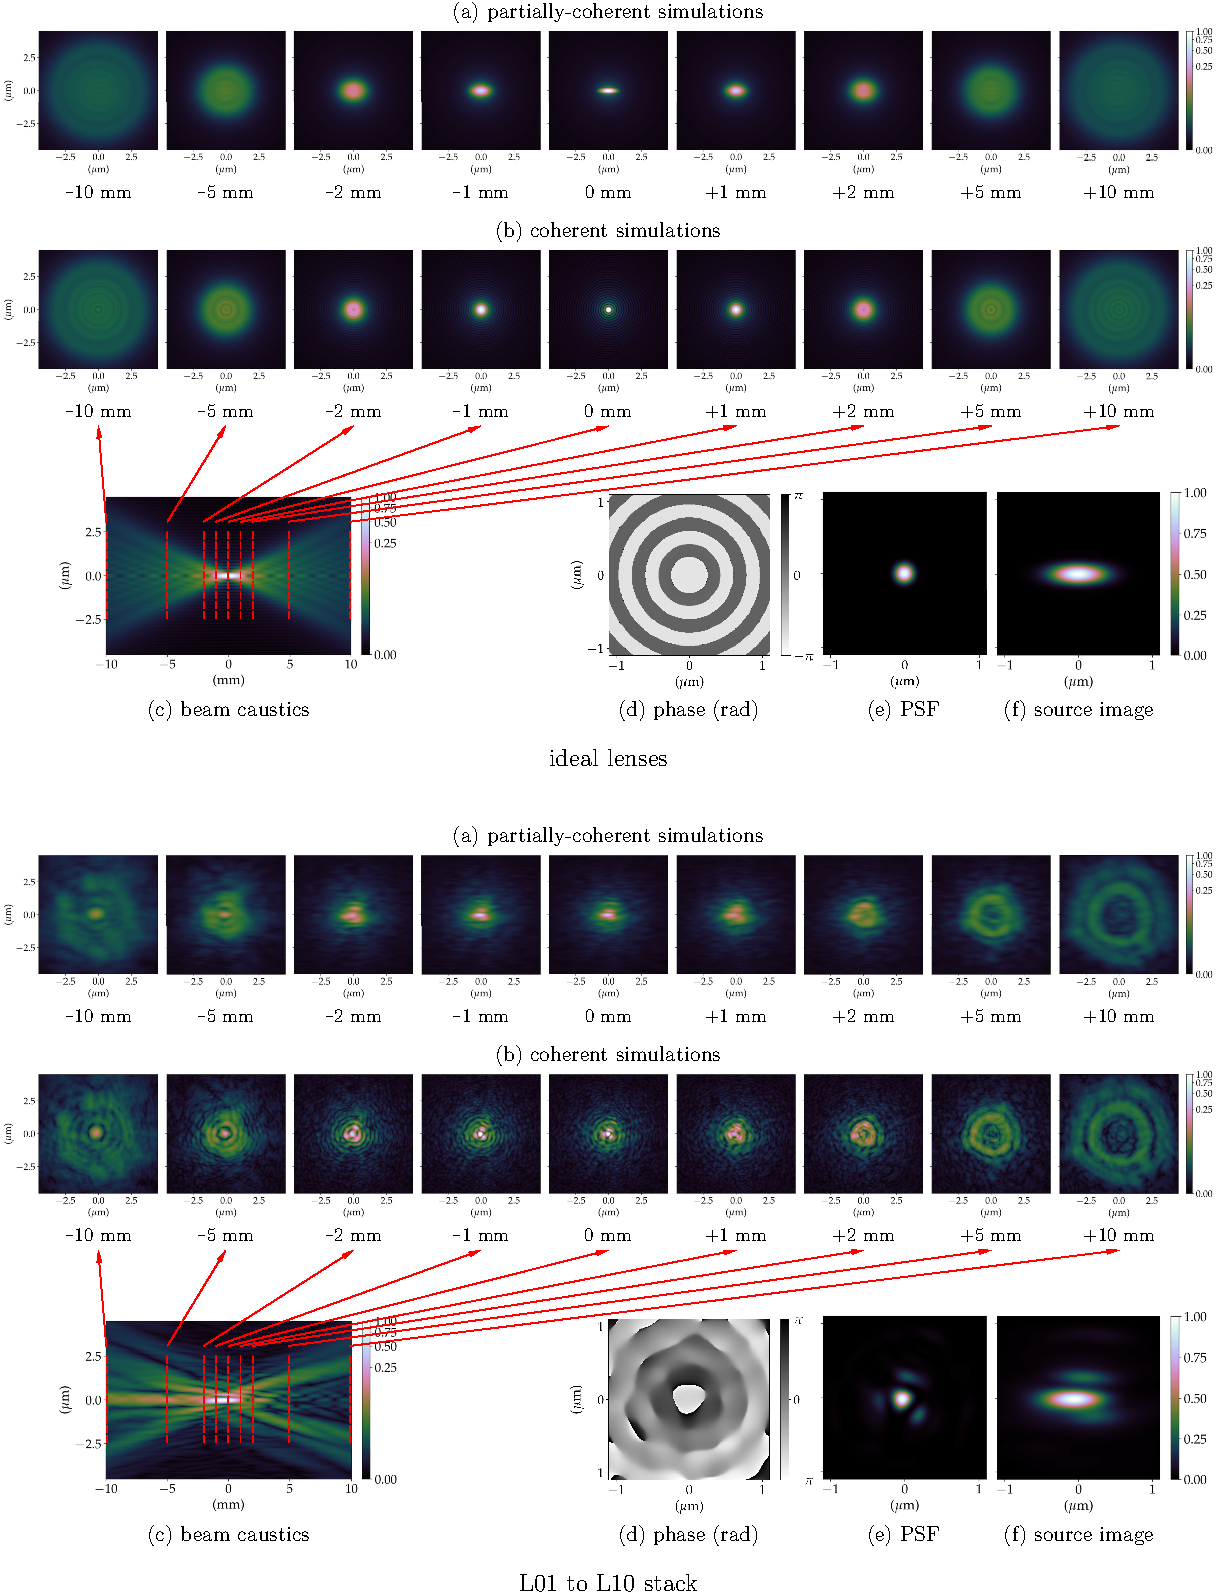
\includegraphics[width=0.99\linewidth]{figures/ch05/CDn.pdf}}
        \caption[L01-L10 studied under fully- and partially-coherent illuminations]{Lens stack formed by individually measured lenses L01-L10 studied under fully- and partially-coherent illumination. (a) partially-coherent simulations show the beam profile up- and downstream the focal position averaging 10$^{4}$ wavefronts to simulate the radiation emitted by an undulator; (b) the coherent simulations show the beam profile of a plane wavefront being focused; (c) beam propagation near the focal position (beam caustics) for a fully coherent beam (horizontal cut around $y=0$); (d) phase and (e) intensity of the PSF calculated focusing a plane-wavefront; (f) demagnified image of the undulator photon-source (extended source). The simulated CRLs are composed of 10 2D-Beryllium lens with nominal radius $R=50~\mu\text{m}$, geometric aperture $A_{\diameter}=440~\mu\text{m}$ and $t_\text{wall}=20~\mu$m at 8~keV. The error profiles used are shown in Fig.~\ref{fig:accumulated_profile_1}.}\label{fig:CDnS}
\end{figure}

\clearpage

%-------------------------------------------------------------------------
%-------------------------------------------------------------------------
\section{Imaging}\label{sec:imaging_sim}
%-------------------------------------------------------------------------
%-------------------------------------------------------------------------
\todo{If there's time: grid \& Siemens star [\cite{Simons2017}]} 
%-------------------------------------------------------------------------
%-------------------------------------------------------------------------
\section{Discussion}\label{sec:discussion}
%-------------------------------------------------------------------------
%-------------------------------------------------------------------------

The main results drawn from the simulations presented previously are discussed in this section. Firstly, some considerations on the effect of optical imperfections on a (partially) coherent X-ray beam are drawn. The merit of using the Strehl ratio for X-ray lenses tolerancing is also discussed. Finally, some comments on the simulation times are done.

%-------------------------------------------------------------------------
%-------------------------------------------------------------------------
\subsection{Metrology of individual lenses vs. stacked lenses}\label{sec:stacking}
%-------------------------------------------------------------------------
%-------------------------------------------------------------------------

The metrology of single lenses and that of lens stacks was already discussed in \S\ref{sec:metrology}~-~\textit{\nameref{sec:metrology}}. The qualitative agreement between the obtained profiles from the measurement of a lens stack and the individually measured and artificially stacked lenses is shown in Figs.~\ref{fig:accumulated_profile_1}-\ref{fig:CDo} and Tables~\ref{tab:CDn} and \ref{tab:CDo}. This qualitative agreements is transferred to the simulations as evidenced by Figs.~\ref{fig:CDn_vs_CDnStack} and \ref{fig:CDo_vs_CDoStack}. Both set of simulations, that is L01-L10 vs. stack 1 and L11-L20 vs. stack 2, show good agreement for the beam caustic, PSF and source image. The lenses L11-L20 and stack 2 show a lower degree of similarity partially-coherent simulation as shown in Fig.~\ref{fig:CDo_vs_CDoStack}(d). This can be attributed to the lenses/stack alignment (positioning) in the when performing the lenses metrology and subsequent software stacking. Figure~\ref{fig:CD_Strehl} shows the Strehl ratio for both coherent and partially-coherent simulations for this sets of simulations. The coherent Strehl ratio shows very good agreement in terms of beam profile for both sets, despite the difference in intensity for the L11-L20 simulations. The L01-L10 simulations preserve the agreement on the partially-coherent simulations, but the L11-L20 set shows more difference between the individually measured lenses and the stack - see also Fig.~\ref{fig:CDo_vs_CDoStack}(d), but the general beam profile is maintained. When comparing the results in Fig.~\ref{fig:CD_Strehl} with the predicted Strehl ratios in Table~\ref{tab:Strehl}, it is evident the large discrepancy seen in the simulations of the L01-L10 lenses (individually measured and stack). It is predicted that the simulations using the metrology data from the lens stack (as opposed to the individually measured lenses) would have a much lower intensity due to a higher figure error value across the pupil, which is not observed. Although a deeper discussion on the Strehl ratio is presented in \S\ref{section:discussion_strehl}~-~\textit{\nameref{section:discussion_strehl}}, it merits to say that the probable cause for this comes from the fact that the Strehl ratio predictions from Eqs.~\ref{eq:Strehl}-\ref{eq:Mahajan} were applied without weighing the errors with the beam transmission for this system - see Fig.~\ref{fig:EffectiveAperure}. The stack measurement has a smaller effective aperture and the error values towards the edge tend to be large and to be misrepresent when providing a single metric such as a rms value for the figure error $\sigma_z$. This does not seem to be the case for the lens stack 2.

\begin{figure}[t]
    \centering
    {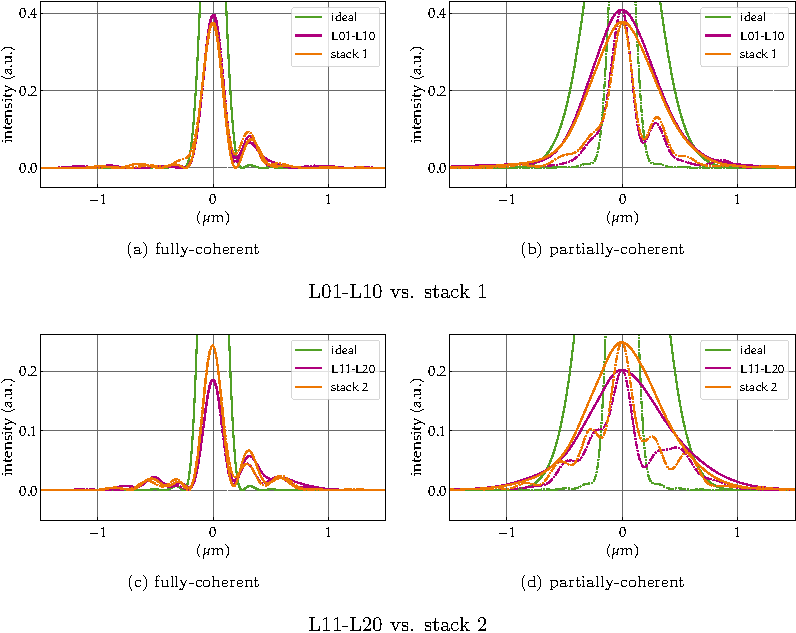
\includegraphics[width=0.7\linewidth]{figures/ch05/CD_Strehl.pdf}}
    \caption[Strehl ratio of L01-L10 vs. stack 1 and L11-L20 vs. stack 2 simulations]{Graphical representation of the Strehl ratio for the profiles in Figs.~\ref{fig:accumulated_profile_1}-\ref{fig:CDn} (\textbf{top row}) and the for the profiles in Figs.~\ref{fig:accumulated_profile_2} and \ref{fig:CDo} (\textbf{bottom row}) at 8~keV. }
    \label{fig:CD_Strehl}
\end{figure}

The effect on the resulting aberrations of stacking X-ray lenses has been modelled and discussed in depth by [\cite{Osterhoff2017}]. The progressive increase in the resulting figure errors from lenses artificially stacked is shown in Fig.~\ref{fig:stacking_errors}, which shows the evolution of the (a) full figure errors, (b) the polynomial fit of the full profile and (c) the residues when stacking lenses \todo{carefully read Osterhof's paper and make comparison with his theory}. The simulations in Fig.~\ref{fig:CDn01-05-10} show the progressive deterioration of an X-ray beam by adding the figure errors to the simulations by showing three scenarios: a single lens, five lenses and ten lenses, representing a low-, a moderate- and a high-aberrated system. This sensitivity study in only possible because the metrology of individual lenses is available. Using the metrology of a full stack and scaling it would not adequately represent the system due to the existence of correlated- and uncorrelated figure errors as pointed out by [\cite{Osterhoff2017}] and shown in Fig.~\ref{fig:stacking_errors}.


\begin{figure}[t]
    \centering
    {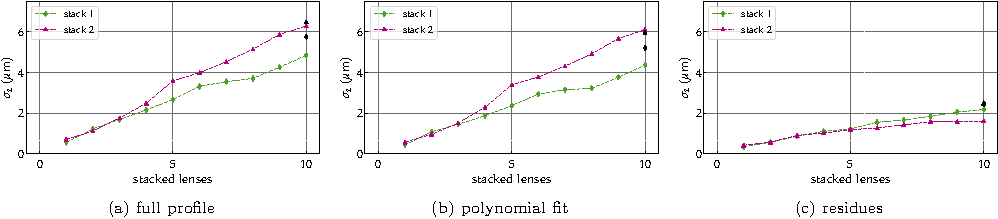
\includegraphics[width=1.\linewidth]{figures/ch04b/stacking_errors.pdf}}
    \caption[Accumulative figure errors]{Progressive increase of figure errors for the (a) full-, (b) fit- and (c) residual- profiles. The green-diamond shaped marker indicates the artificially stacked lenses from the stack 1, while the magenta triangles, the stack 2. The black markers indicate the corresponding measured stack. Figure errors calculated for a geometric aperture of $A_{\diameter}=400~\mu\text{m}$.}
    \label{fig:stacking_errors}
\end{figure}

%-------------------------------------------------------------------------
%-------------------------------------------------------------------------
\subsection{The effect of optical imperfections}\label{section:discussion_imperfections}
%-------------------------------------------------------------------------
%-------------------------------------------------------------------------

Applying the Mar\'echal criterion (Eq.~\ref{eq:MarechalCriterion}) calculated for Beryllium lenses illuminated at 8~keV requires the accumulated projected figure errors to be $\sigma_z\leq2.08~\mu\text{m}$. Tables~\ref{tab:CDn} and \ref{tab:CDo} show that the accumulated thickness for both stacks is larger and that the optical system is operating far from ideal as the system exceeds the limit imposed by the Mar\'echal criterion. The decomposition of the figure error profiles into orthonormal polynomials and their resulting residuals is convenient, because it allows to investigate the effects of specific frequency ranges in the X-ray beam degradation. Following [\cite{Harvey1995a}], the figure errors of the lenses can be specified in terms of their spatial frequency, as they often have different effects on the image quality. Three regions are commonly used for that: low-, mid- and high-spatial-frequencies. The low-spatial frequencies (LF) are responsible for changing the beam profile and reducing the peak intensity. They are related to the conventional optical aberrations [\cite[\textit{\S9.1-3}]{born_wolf1999}] and they can be described by a set of orthonormal polynomials, which has been described in \S\ref{sec:orthonormal_polynomials}~-~\textit{\nameref{sec:orthonormal_polynomials}}. Mid- and high-spatial frequencies (HF) are responsible for scattering the light around the (focused) beam and have potential for broadening it, together with the expected reduction of the Strehl ratio. The mid- and high- frequencies are the residuals from the polynomial fit of the aberrated profile in this context. The full profile comprises all spatial frequencies and is referred to as FF. From the analysis of the experimental data from 2D-Beryllium lenses with nominal radius $R=50~\mu\text{m}$ and geometric aperture $A_{\diameter}=440~\mu\text{m}$, Zernike circle polynomials until the 37$^\text{th}$ order (3$^\text{rd}$ order spherical aberration) were used. Which causes the low-frequencies (LF) to span from $\sim500~\mu$m or $2\times10^{3}~\text{m}^{-1}$ (geometrical aperture of a lenslet) to $\sim50~\mu$m or $2\times10^{4}~\text{m}^{-1}$, while the mid- and high-frequencies span from $\sim50~\mu$m or $2\times10^{4}~\text{m}^{-1}$ to $\sim0.5~\mu$m or $2\times10^{6}~\text{m}^{-1}$, which is obtained from the Nyquist frequency of the measured data. Figure~\ref{fig:CDnFF_LF_HH} shows the effects of different spatial frequencies ranges on a X-ray beam. 

The addition of the mid- and high-spatial frequency errors to an ideal CRL model is related to scattering around the focused beam, contributing thus to increased background and consequently reducing the peak intensity following [\cite{Harvey1995a}]. Using a linear scale, both the ideal PSF and the demagnified source image in Figs.~\ref{fig:CDn_vs_CDnStack}(c)-(d) are almost indistinguishable from their aberrated counterparts in Figs.~\ref{fig:CDnFF_LF_HH}(c)-(d), which is due to the fact that the accumulated figure error complies to the Mar\'echal criterion. As pointed out by [\cite{Cocco2015, Cocco2019}], a compliant Strehl ratio does not guarantee a homogeneous beam profile up- and downstream of the focal position. This is evident in the beam caustic shown in Fig.~\ref{fig:CDnFF_LF_HH}. The profile shown in Fig.~\ref{fig:CDn}(c) is not random and presents some concentric rings. This comes from the tooling of the punches used in the hot-embossing process of the Be lens fabrication. Using a more diverse profile, such as the one shown in Fig.~\ref{fig:CDnHF}, which also comes from the metrology of real Be lenses artificially stacked, it is clear that introducing random HF errors does not significantly change the beam shape as they contribute to the scattering of light outside the beam envelope defined by the ideal beam caustics - cf. Fig.~\ref{fig:simulations_HF}. 

\begin{figure}[t]
        \centering
        {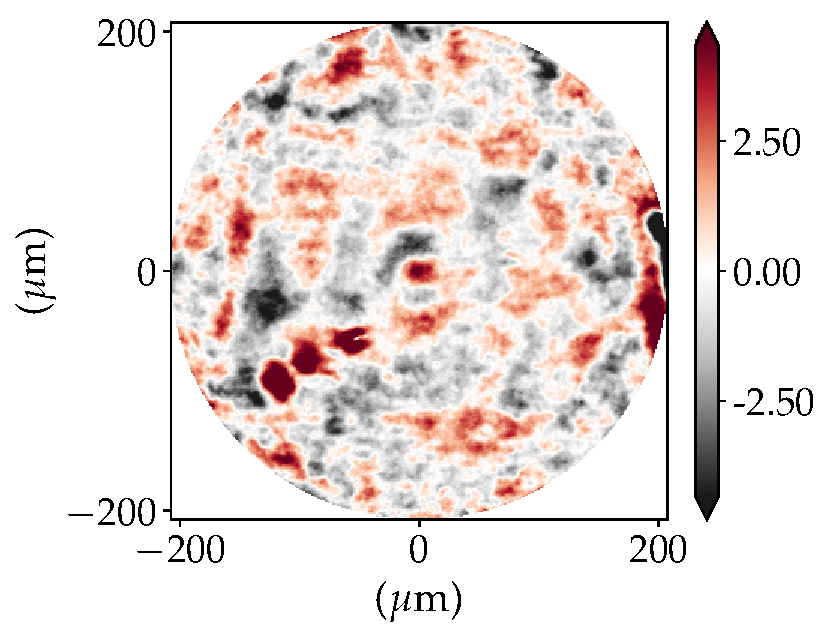
\includegraphics[width=0.3\linewidth]{figures/ch05/CDnHF/phase_n_CRL_errors_residues_phase_figure_errors_FF}}
        \caption[High frequency errors profile]{Artificially stacked high frequency error profile from 10 individually measure 2D-Beryllium lens with nominal radius $R=50~\mu\text{m}$, geometric aperture $A_{\diameter}=440~\mu\text{m}$ and $t_\text{wall}=20~\mu$m used in the simulations shown in Fig.~\ref{eq:Strehl} and Fig.~\ref{fig:simulations_HF}. The profile has a $\sigma_z=1.74~\mu$m.}\label{fig:CDnHF}
\end{figure}

\begin{figure}[t]
        \centering
        {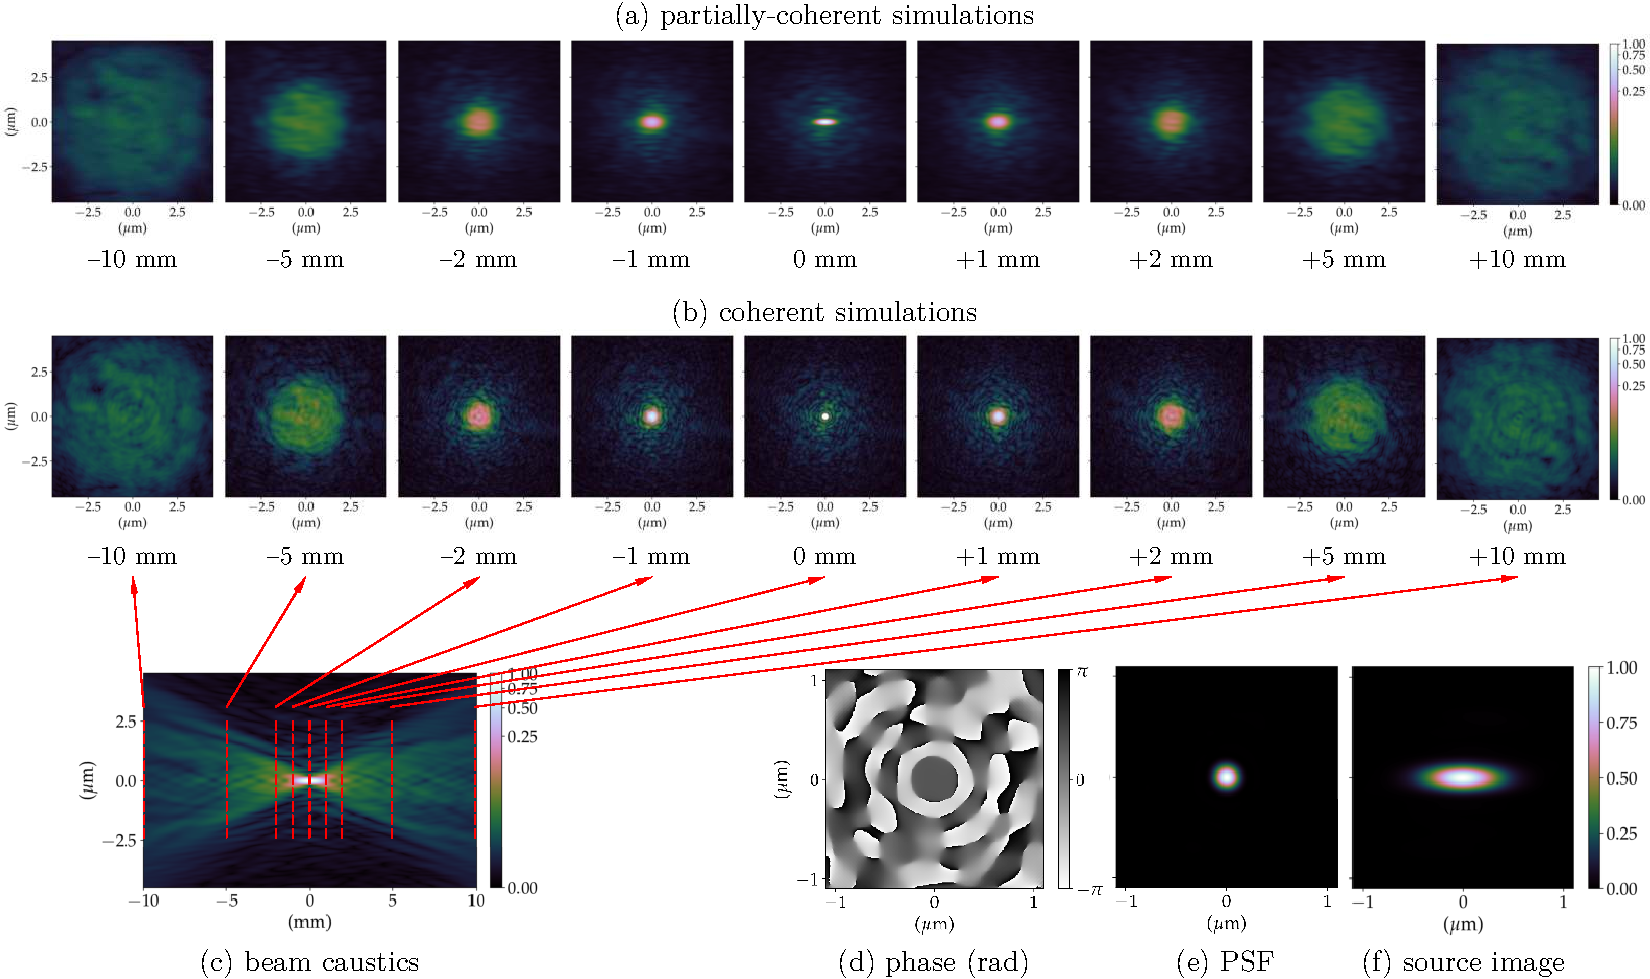
\includegraphics[width=0.99\linewidth]{figures/ch05/CDn_HF.pdf}}
        \caption[High frequency errors studied under fully- and partially-coherent illuminations]{High frequency error profile studied under fully- and partially-coherent illumination. (a) partially-coherent simulations show the beam profile up- and downstream the focal position averaging 10$^{4}$ wavefronts to simulate the radiation emitted by an undulator; (b) the coherent simulations show the beam profile of a plane wavefront being focused; (c) beam propagation near the focal position (beam caustics) for a fully coherent beam (horizontal cut around $y=0$); (d) phase and (e) intensity of the PSF calculated focusing a plane-wavefront; (f) demagnified image of the undulator photon-source (extended source). The simulated CRLs are composed of 10 2D-Beryllium lens with nominal radius $R=50~\mu\text{m}$, geometric aperture $A_{\diameter}=440~\mu\text{m}$ and $t_\text{wall}=20~\mu$m at 8~keV. The error profile used is shown in Fig.~\ref{fig:CDnHF}.}\label{fig:simulations_HF}
\end{figure}

When considering the low-spatial-frequency figure errors, however, the beam shape starts to change more drastically even at the focal position. The appearance of satellite peaks become pronounced in the PSF and the demagnified source image. The beam caustics start presenting an elongated tail-like structure upstream the focal position and a ring-like structure downstream. The elongation of the beam along the optical axis and the presence of homogeneous concentric rings on the PSF are a classical signature of spherical aberration, which is a major component of the LF figure errors - cf. $Z_{11}$ in Figs.~\ref{fig:CDn}(d)-\ref{fig:accumulated_profile_2}(d). The predominance of spherical aberration on 2D parabolic Be lenses has already been observed; see Fig.~6.14 of [\cite{Seiboth2016b}]. The PSF due to spherical aberration can be seen also in Figs.~8.5 and 8.6 from [\cite{Mahajan2011}]. In the partially-coherent simulations, the satellite peaks around the main lobe seen at the PSF simulations are stretched horizontally to the point that their visibility is maintained vertically, but horizontal cuts (Fig.~\ref{fig:CDnFF_LF_HH}(d)) show almost no trace of them, due to the reduction in transverse horizontal coherence (blurring effect). Small misalignments between the lenslets and some residual tilt from the LF errors contribute to a lateral displacement of the beam in the image plane. Using the full-frequency-range figure errors yields a combined effect that is analogous to the superposition of the HF and LF figure errors. The complete set of simulations using lenses L01-L10 using the CRL-MS modelling given by Eq.~\ref{eq:TE_CRL_MS_ERR} can be seen in Fig.~\ref{fig:CDnS}. The diffraction effects from the aperture of the CRL are not easily observable because the system has an apodised Gaussian intensity at the exit pupil [\cite{Mahajan1986}], but they contribute to the concentric ring structures seen on the ideal lenses simulation in Fig.~\ref{fig:CDnS}.

The simulations shown in Figs.~\ref{fig:CDn_vs_CDnStack}-Fig.~\ref{fig:CDnS} paint a very consistent picture of the beam shape along the optical axis. Upstream of the image plane, a persistent central lobe is observed, albeit much less intense, with a high background around it thus reducing the signal to noise ratio. Downstream, the beam has a drop in intensity in the middle, looking like a doughnut when a cut transverse the optical axis is made. This behaviour is observed both on fully- and partially-coherent simulations and is more evident in the simulations shown in Fig.~\ref{fig:CDnS} (beam profiles). Such beam caustics have been extensively reported by experimental groups working under high coherent conditions, with similar optics and ptychographic reconstruction of X-ray beams - cf. Fig.~3 in [\cite{Schropp2013}], Fig.~2 in [\cite{Seiboth2016}], Fig.~3 in [\cite{Gasilov2017}] and Fig.~4 in [\cite{Seiboth2020}].


\begin{figure}[t]
    \centering
    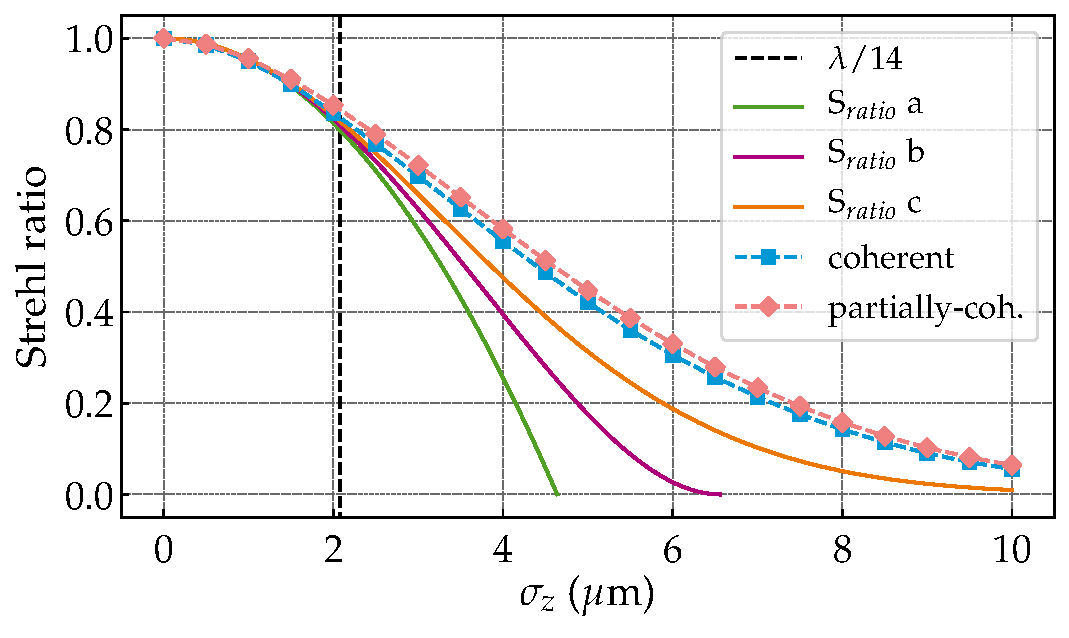
\includegraphics[width=7.5cm]{figures/ch05/fig_10.pdf} %trim = left bottom right top
    \caption[Strehl ratio from numerical simulations]{Strehl ratio from numerical simulations and from the application of different approximations (Eqs.~\ref{eq:Strehl}-\ref{eq:Mahajan}) as a function of the figure error $\sigma_z$ from a lens stack made of Beryllium illuminated at 8~keV. The vertical dashed black line indicates the maximum tolerable thickness error (Eq.~\ref{eq:ThickLim}) for complying with the Mar\'echal criterion (Eq.~\ref{eq:MarechalCriterion}), that is, $\sigma_{\lambda/14}\approx2.08~\mu\text{m}$. The partially-coherent simulations were done with 10$^{4}$ wavefronts.}
    \label{fig:Strehl}
\end{figure}{}

%-------------------------------------------------------------------------
%-------------------------------------------------------------------------
\subsection{The Strehl ratio for X-ray lenses}\label{section:discussion_strehl}
%-------------------------------------------------------------------------
%-------------------------------------------------------------------------

The Strehl ratio for the CRL models is presented in Table~\ref{tab:Strehl}. In the numerical simulations, the intensity at the centre of the beam is normalised to the intensity obtained by the ideal model. What is generally observed is that for values lower than the  Mar\'echal criterion (Eq.~\ref{eq:MarechalCriterion}), the analytic equations Eqs.~\ref{eq:Strehl}-\ref{eq:Mahajan} show a good agreement and can be used to estimate the performance of an optical system close to the ideal performance. However, for moderate or strong values of aberrations the approximations used to derive those equations start to break down and other factors have to be taken into account, such as spatial distribution of the error profile and the transmission profile across the exit pupil. The values shown on Table~\ref{tab:Strehl} do not show a clear trend when it comes to the Strehl ratio and the rms value of the figure error across the exit pupil of the system. In order to understand the numerically dependence of the Strehl ratio on the height error, each individual profile used to generate the profile shown in Fig.~\ref{fig:CDnHF} was scaled by a constant value to allow for a scanning of the total projected figure error $\sigma_z$. The results in Figure~\ref{fig:Strehl} show the expected Strehl ratio as a function of the projected figure errors $\sigma_z$ for different analytical approximations (Eqs.~\ref{eq:Strehl}-\ref{eq:Mahajan}) and for the numerical calculations with a fully- and partially-coherent illumination. All approaches show very good agreement up to $S_\text{ratio}>0.8$, when they start diverging. The expressions for $S_\text{ratio a}$ (Eq.~\ref{eq:Strehl}) and  $S_\text{ratio b}$ (Eq.~\ref{eq:Marechal}) can be considered as approximations for $S_\text{ratio c}$ (Eq.~\ref{eq:Mahajan}), therefore are only expected to be valid over a restricted range (large $S_\text{ratio}$). A fit of the simulation data (coral rhombuses and blue squares in Fig.~\ref{fig:Strehl}) give:
\begin{subequations}\label{eq:Strhel_Exp_pre}
\begin{align}
    S_{\text{ratio coh.}}&\approx\exp{\big(-2.32\cdot10^{10}\sigma_z^2 -6.13\cdot10^4\sigma_z + 2.54\cdot10^{-2}\big)},\\
    S_{\text{ratio part.-coh.}}&\approx\exp{\big(-2.28\cdot10^{10}\sigma_z^2 -5.07\cdot10^4\sigma_z + 2.29\cdot10^{-2}\big)}.
\end{align}
\end{subequations}
Unfortunately, due to the nature of the projected figure errors (in the range of few micrometres r.m.s.), it is not possible to discard the non-quadratic terms. Equations~\ref{eq:Strhel_Exp_pre} can be rewritten as:
\begin{align}\label{eq:Strhel_Exp}
    S_{\text{ratio simulation}}&\approx\exp{\bigg[- \bigg(\frac{2\pi}{\lambda}\bigg)^2\big(\kappa_1\Delta\Phi\big)^2-\frac{2\pi}{\lambda}\kappa_2\Delta\Phi-\kappa_3\bigg]},
\end{align}
where $\kappa$ are scaling constants that, in principle, the number of elements, lens material, energy and, mostly importantly, the spatial distribution of the accumulated errors over the optical element aperture. For our particular examples, $\kappa_1=0.71$, $\kappa_2=0.28$ and $\kappa_3=2.54\cdot10^{-2}$ for the coherent case and $\kappa_1=0.70$, $\kappa_2=0.24$ and $\kappa_3=2.29\cdot10^{-2}$ for the partially-coherent case. When comparing Eq.~\ref{eq:Strhel_Exp} with Eq.~\ref{eq:Mahajan}, a $\kappa<1$ suggests that there is some weighting of the phase errors reducing their effect, but simply multiplying the accumulated thickness errors (cf. Figs.~\ref{fig:CDn}-\ref{fig:accumulated_profile_2}) with the normalised optical system transmission (cf. Fig.~\ref{fig:EffectiveAperure}) does not allow prediction of $\kappa$ and this is still as an open question at the time of writing, which strengths the case for the simulation framework developed for this thesis.

Following the recent discussion about the pertinence of the $S_\text{ratio}\geq0.8$ as an indicator of optical quality for the X-ray regime and the performance of such optical systems away from the focal position [\cite{Cocco2015, Cocco2019}], it can be observed from Fig.~\ref{fig:CDnS} that in terms of wavefront preservation, X-ray lenses are more susceptible to the low-frequency figure errors, as they are the ones that change the beam profile up- and downstream the focal position. The high-frequency errors lead to scattering of the beam and speckles, but generally, do not change the beam shape even away from the focal position. It is clear from Fig.~\ref{fig:CDnS} that the Strehl ratio encountered at the focal position (cf. Fig.~\ref{fig:CD_Strehl}) is not preserved up- or downstream from it due the distored beam shape. Fortunately, the low frequencies are those which can be readily corrected by the fitting of corrective optics - which will be discussed in \S\ref{sec:corrections}~-~\textit{\nameref{sec:corrections}}. 

\subsection{Simulation time}\label{section:discussion_time}

Increasing the complexity of the simulation model comes at the expense of increasing the overall simulation time, but as long as the transverse wavefront sampling is maintained, memory consumption is not affected from one model to another. The time increase in the simulations is mainly due to: \textit{i}) increase in the number of drift spaces and the number of optical elements; \textit{ii}) from reading the densely sampled metrology data. Table~\ref{tab:simulation_time} presents the typical simulation times for this work. Those are particularly high because the transverse sampling of the wavefronts is several times larger than the nominal minimal sampling necessary to mitigate artefacts or under-resolved features on the wavefront. Employing 10$^{4}$ wavefronts for the partially coherent simulations is also exaggerated, but was done to ensure that any changes on the simulation come from the change of model being studied and not from statistical nature of the sampling of the electron-beam phase-space. The simulation times presented on Table~\ref{tab:simulation_time} can be certainly be reduced without loss of accuracy by adopting a more sensible sampling. $\blacksquare$

\begin{table}[t]
\caption[Summary of the simulation times for different CRL models]{Summary of the simulation times for different CRL models. From the most simple one (single lens equivalent) up to the more complex multi-slicing (MS) with figure errors. Simulations were performed on a Intel(R) Xeon(R) CPU E5-2680 v4 @ 2.40GHz cluster at the ESRF. Partially coherent calculations were done using 28 cores in parallel.}\label{tab:simulation_time}\small
\centering
\begin{tabular}{rccc}\hline\hline
\multicolumn{1}{c}{\textbf{model}} & \textbf{fully coherent} &\textbf{ partially coherent} & \textbf{caustics}\\\cline{1-4}
single lens equivalent (Eq.~\ref{eq:TE_CRL})                 &33~s            &2~h~44~min  &1~h~32~min               \\
multi-slicing  (Eq.~\ref{eq:TE_CRL_MS})                     &58~s            &5~h~12~min  &1~h~33~min               \\
MS + figure errors  (Eq.~\ref{eq:TE_CRL_MS_ERR})                &2~min~48~s      &5~h~42~min  &1~h~35~min               \\\cline{2-4}
\multicolumn{1}{c}{}               & (1 wavefront)  & (10$^{4}$ wavefronts)  & (4001 pts.) \\\hline\hline
\end{tabular}
\end{table}











\addcontentsline{toc}{section}{References}
\printbibliography[heading=subbibliography]
\end{refsection}

 \cleardoublepage
% 15/11/2020 - First round of corrections: added Thomas (new) & Ray corrections
% 15/11/2020 - Grammarly

\begin{refsection}
\chapter{Correcting optical imperfections in refractive lenses}\label{sec:corrections}

The interest and possibility of arbitrarily manipulating the X-ray wavefront has been teased since, at least, the early 2000s [\cite{Chubar1999, Chubar2001b}]. It was not until the advent of extremely accurate additive and subtractive manufacturing techniques [\cite{Stohr2015, Polikarpov2016, Petrov2017, Roth2018, Sanli2018, Seiboth2019, Abrashitova2020, Antipov2020, Lin2020, Medvedskaya2020}] that the demonstration of free-form X-ray refractive optics was done [\cite{Sawhney2016,Seiboth2017,Laundy2019, Seiboth2020, Dhamgaye2020}]. The possibility of producing very accurate free-form optics for the correction of optical aberrations has brought renewed interest in wavefront sensing [\cite{Berujon2015, Seaberg2019}] and optical design simulations [\cite{Laundy2020}]. This chapter presents the early results on correcting optical imperfections in refractive lenses obtained at the ESRF. The design and expected performance is based on the lenses presented in \S\ref{sec:single_lens}~-~\textit{\nameref{sec:single_lens}} and the simulations shown in Chapter~\ref{sec:effect_optical_imperfections}~-~\textit{\nameref{sec:effect_optical_imperfections}}.

%-------------------------------------------------------------------------
%-------------------------------------------------------------------------
\section{Corrective optics}\label{sec:corrective_optics}
%-------------------------------------------------------------------------
%-------------------------------------------------------------------------

Correcting optical imperfections can be done by actively reshaping an optical element (adaptive optics) [\cite{Sutter2012, Alcock2013}] or by inserting a static (passive) optical element specially fitted to compensate the deviations from a perfect profile or the wavefront error in relation to an idealised intensity [\cite{Donato2020}] or phase profile. Phase manipulation for wavefront manipulation can be done with diffractive elements [\cite{Probst2020}] or with refractive elements [\cite{Sawhney2016,Seiboth2017,Laundy2019,Seiboth2020, Dhamgaye2020}]. As indicated by the vast literature, refractive optics is the most popular method for correcting phase errors in partially-coherent X-ray beams. This section presents the design of refractive optical correctors for refractive lens stacks.

%-------------------------------------------------------------------------
%-------------------------------------------------------------------------
\subsection{Design}\label{sec:design}
%-------------------------------------------------------------------------
%-------------------------------------------------------------------------
\begin{figure}[t]
        \centering
        {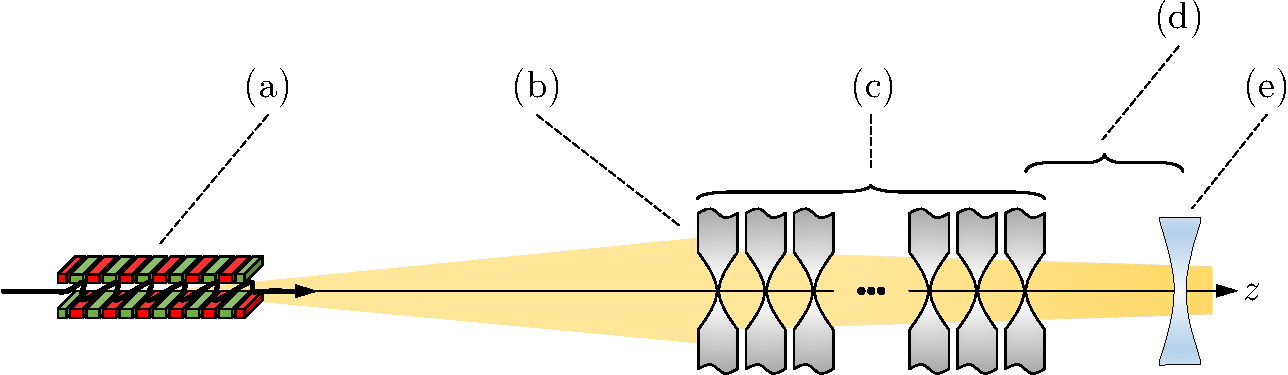
\includegraphics[width=0.6\linewidth]{figures/ch06/phase_extraction.pdf}}
        \caption[Schematic for phase correction calculation]{Schematic for residual phase extraction. (a) an arbitrary X-ray source delivers a (b) wave-field $U_{\text{illum.}}(x,y)$ immediately before the (c) optical system being studied. The wave-field exits the optical system and can be propagated a (d) distance $\Delta_{z_\text{pp}}$ from the exit pupil. At this position, the (e) extraction of the ideal phase from $U_{\text{exit}}(x,y)$ is done according to Eq.~\ref{eq:phase_corr}.}\label{fig:phase_extraction}
\end{figure}
Formally, the computation of the phase correction\footnote{The design of optical correctors for synchrotron radiation was first described in [\cite[\textit{§2}]{Chubar1999}], revisited in [\cite{Chubar2001b}] and first implemented for a 2D CRL in [\cite{Seiboth2017}].} for any optical system is done by assuming that the wave-field will develop a specific phase $\phi_{\text{exit}}(x,y)$ distribution after passing through an arbitrary optical system. Perfect focusing of a wave-field to a point-source at a distance $r$ from the exit pupil requires that the developed phase $\arg [U_{\text{exit}}(x,y)]$ to be that of a spherical-wave as in Eq.~\ref{eq:spherical} [\cite{Chubar1999}]. Given the typical geometric apertures and focal distances of a CRL composed of a few individual lenses\footnote{Assuming that the focusing inside the CRL is negligible - cf. [\cite{Schroer2005}] and [\cite[\textit{\S6}]{Seiboth2018}].}, it is possible to use the phase of the paraxial approximation of Eq.~\ref{eq:spherical}, that is, the parabolic-phase of the wavefront in Eq.~\ref{eq:parabolic}. If the wavefront illuminating the optical system is given by $U_{\text{illum.}}(x,y)$, then, after passing through an aberrated lens system, $U_{\text{exit}}(x,y)$ is given by:
\begin{equation}\label{eq:U_exit}
    U_{\text{exit}}(x,y) =   \mathcal{D}(\Delta_{z_\text{pp}})\cdot\left[\mathrm{T}_{\text{CRL-MS}}(\Delta_z) \cdot U_{\text{illum.}}(x,y)\right],
\end{equation}
where $\mathcal{D}(\Delta_{z_\text{pp}})$ is a free-space propagation from the exit pupil of the optical system to the position along the optical axis where the phase correction is performed (Eq.~\ref{eq:Fresnel_operator}) and $\mathrm{T}_{\text{CRL-MS}}(\Delta_z)$ is the operator description of a lens stack given by Eq.~\ref{eq:TE_CRL_MS_ERR}. The phase shift necessary to correct such wavefront can be calculated as:
\begin{equation}\label{eq:phase_corr}
   \phi_{\text{correction}}(x,y) = \arg\left[\cfrac{\exp{\Big(-ik\frac{x^2 + y^2}{2z_f}\Big)}}{U_{\text{exit}}(x,y)}\right].
\end{equation}
Where $z_f$ is the distance from the phase corrector to the image plane [\cite{Seiboth2017}]. This phase extraction procedure is illustrated in Fig.~\ref{fig:phase_extraction}. A phase corrector based on refractive optics can be calculated directly from the phase obtained in Eq.~\ref{eq:phase_corr} and the transmission element in projection approximation phase-thickness relationship described by Eq.~\ref{eq:aux_funcs_transb}:
\begin{equation}\label{eq:phase_plate}
   \Delta_\text{pp}(x,y)=-\frac{\phi_{\text{correction}}(x,y)}{k\delta_\text{pp}(x,y)}.
\end{equation}
Where $\Delta_\text{pp}(x,y)$ is the local phase plate thickness in projection approximation and $\delta_\text{pp}$ is the refraction index decrement of the material used for correcting $ \phi_{\text{exit}}(x,y)$. The resulting correction plate described by Eq.~\ref{eq:phase_plate} is directly proportional to the phase errors at each $(x,y)$ coordinate pair. Typical error maps are shown in Figs.~\ref{fig:metrology_zernike_profiles}, \ref{fig:recovered_thickness}, \ref{fig:accumulated_profile_1}-\ref{fig:CDo}. Current micro- and nanofabrication techniques used for manufacturing X-ray optics\footnote{Current for micro- and nanofabrication of 3D structures include: } are capable of reproducing such intricate shapes with high spatial and depth resolution, however the use of such correction plate in an experimental setup is rather impractical due to the several degrees of freedom concerned when aligning it against the aberrated optical system. Furthermore, it has been observed that 2D lenses produced by (hot) embossing are dominated by spherical aberration terms (primary, secondary, tertiary...) and other azimuathally symmetric errors due to intrinsic manufacturing processes [\cite{Schropp2013, Uhlen2014, Seiboth2016, Seiboth2017, Celestre2020, Seiboth2020}] -  see also the Zernike polynomial bar plots (orange bars) in Figs.~\ref{fig:metrology_zernike_profiles}, \ref{fig:recovered_thickness}, \ref{fig:accumulated_profile_1}-\ref{fig:CDo}. Trading some of the correction accuracy for more practicality when employing the correction plate in a beamline, it is possible to obtain a correction profile by azimuthally averaging $\Delta_\text{pp}(x,y)$:
\begin{equation}\label{eq:phase_plate_r}
   \Delta_\text{pp}(r)=\cfrac{\displaystyle\int\limits_{0}^{2\pi}{\Delta_\text{pp}(r,\theta)r\text{d}\theta}}{\displaystyle\int\limits_{0}^{2\pi}{r\text{d}\theta}},
\end{equation}
where $r=\sqrt{x^2 + y^2}$ and $\theta=\arctan{\big(y/x\big)}$ are the transformation from Cartesian to polar coordinates. The correction plate as calculated by Eqs.~\ref{eq:phase_plate} and \ref{eq:phase_plate_r} is tailored for a specific set of lenses operating at a defined energy, due to the dispersion properties of $\delta_\text{pp}$. Although true that a correction plate design is suited to a specific lens combination, for a moderate number of lenses where the focusing inside the CRL can be neglected, it has been demonstrated that the correction plate can be used over a range of energies around the design energy $\text{E}_\text{design}$ as the index of refraction decrement $\delta$ is proportional to $\lambda^2$ [\cite[\textit{\S6}]{Seiboth2018}]. This can be done by shifting the plate along the optical axis closer or further away from the design position $\Delta_{z_\text{pp}}$ if the new operation energy is lower or higher than $\text{E}_\text{design}$. The same considerations on the beam chromaticity in \textit{Chromatic aberrations} in \S\ref{sec:CRL_performance}~-~\textit{\nameref{sec:CRL_performance}} apply to the phase correctors. 


%-------------------------------------------------------------------------
%-------------------------------------------------------------------------
\subsubsection*{Materials}
%-------------------------------------------------------------------------
%-------------------------------------------------------------------------

It is natural to envision adopting the same materials used in X-ray lenses for the phase correctors. As for the lenses, the material used for the phase plate is intimately connected to the manufacturing process. Phase plates for optical correction have been produced using fused silica [\cite{Seiboth2017}], diamond [\cite{Polikarpov2016, Antipov2020}] and sapphire [\cite{Lin2020}], manufactured with laser ablation or ion-beam lithography [\cite{Medvedskaya2020}] (subtractive manufacturing); and polymeric resists such as SU-8 (commonly used in LIGA [\cite{Nazmov2004}] and other polymeric lenses [\cite{Stohr2015}]) and the proprietary IP-S used in additive manufacturing via two-photon polymerisation [\cite{Petrov2017, Sanli2018, Abrashitova2020,Lin2020}]. 


%-------------------------------------------------------------------------
%-------------------------------------------------------------------------
\subsection{Correction phase plate calculation}\label{sec:cpp_calculation}
%-------------------------------------------------------------------------
%-------------------------------------------------------------------------

Applying the correction plate design methodology (Eqs.~\ref{eq:U_exit}-\ref{eq:phase_plate_r}) to the individually measured and artificially stacked lenses L01-L10, which have been studied in depth - see Table.~\ref{tab:CDn} and Figs.~\ref{fig:accumulated_profile_1}, \ref{fig:CDn_vs_CDnStack} and \ref{fig:CDnS}; it is possible to recover a phase plate that will improve the performance of that particular optical system. An optical corrector to be used 10~mm downstream of the last lens of the stack, made of diamond and designed to operate at 8~keV is shown (cut) in Fig.~\ref{fig:plate_profile}. Due to the process described by  Eq.~\ref{eq:phase_plate_r}, the profile of the corrective plate is smooth and does not have high spatial-frequency components. The obtained profile is similar to the ones reported in [\cite{Seiboth2017,Seiboth2018,Seiboth2020}], which were obtained for stacks composed of similar lenses. The correction plate was designed using diamond due to its relatively large refractive index decrement $\delta_\text{C*}$ at the expense of a higher absorption, good thermal and mechanical properties and volume homogeneity which translates into low X-ray small-angle scattering when compared to beryllium lenses [\cite{Chubar2020}]. These properties make diamond a very interesting material for (refractive) X-ray optics [\cite{Polikarpov2016b,ShvydKo2017}].

Using the optical setup shown in Fig.~\ref{fig:recovered_phase_corrected}, it is possible to recover the residual figure error profile after the correction plate, as shown in Fig.~\ref{fig:residual_profile}(a) and described in Table~\ref{tab:corrected}. The profiles in Fig.~\ref{fig:residual_profile}(b)-(c) are substantially changed from the Fig.~\ref{fig:accumulated_profile_1}(b)-(c). The polynomial fit in Fig.~\ref{fig:residual_profile}(b) has virtually no spherical aberration terms. The concentric rings from the pressing tool apparent in Fig.~\ref{fig:accumulated_profile_1}(c) are completely removed from the residual errors in Fig.~\ref{fig:residual_profile}(c). Figure~\ref{fig:recovered_phase_corrected}(d) reinforces the observation of the reduction in the figure errors by the use of a azimuthally symmetric phase plate. The radially symmetric components (orange bars) in Fig.~\ref{fig:recovered_phase_corrected}(d) are almost completely removed, while the purple bars remain almost unchanged. Finally, Fig.~\ref{fig:recovered_phase_corrected}(e) shows a residual profile that is several times smaller than the one in Fig.~\ref{fig:accumulated_profile_1}(e).

\begin{figure}[t]
        \centering
        {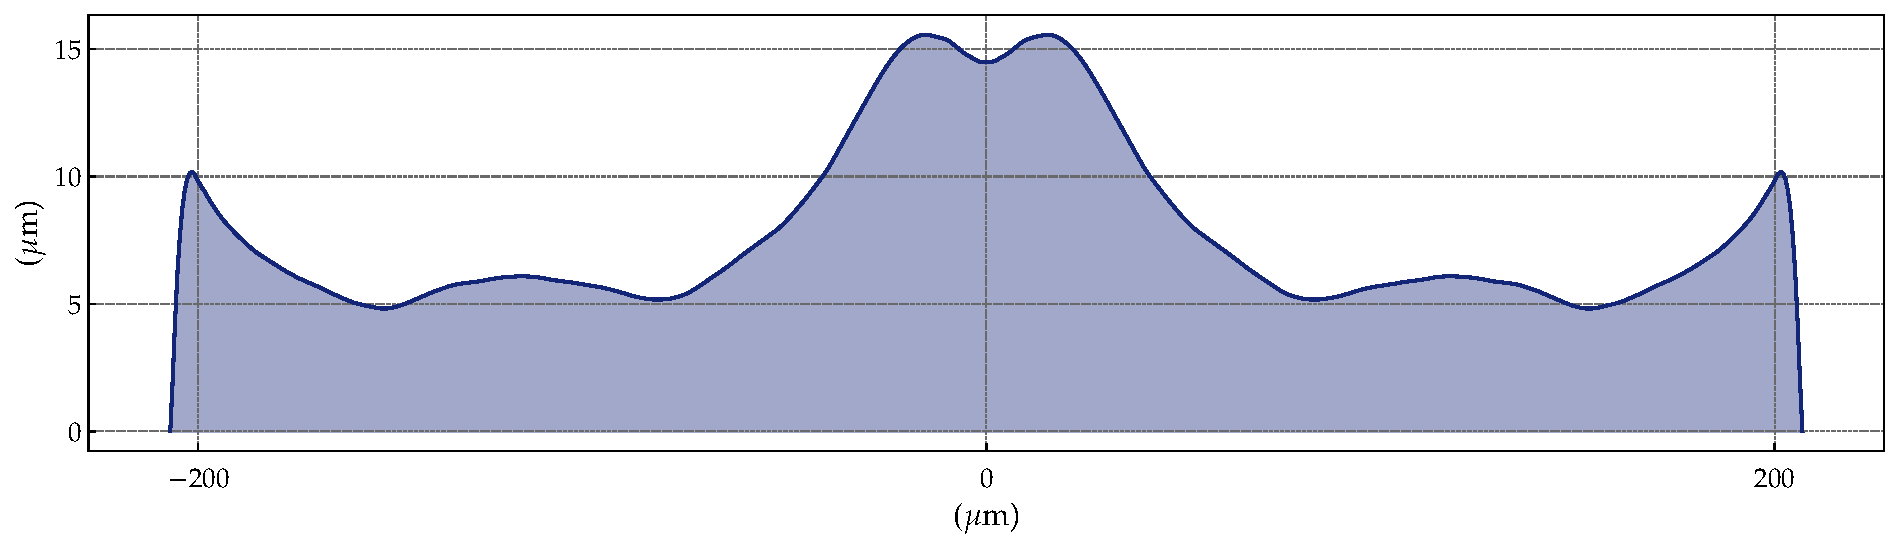
\includegraphics[width=0.6\linewidth]{figures/ch06/CDn_individual_8p0keV_n_10.0_lsp2p0mm_cpp10p0mm_phase_correction_plate_cut_2.pdf}}
        \caption[Diamond correction plate profile cut]{Profile cut of a diamond corrective plate for the lenses L01-L10 at 8~keV - cf. Fig.~\ref{fig:accumulated_profile_1}. The correction plate was calculated 10~mm downstream of the exit pupil of the CRL.}\label{fig:plate_profile}
\end{figure}

\begin{figure}[t]
        \centering
        {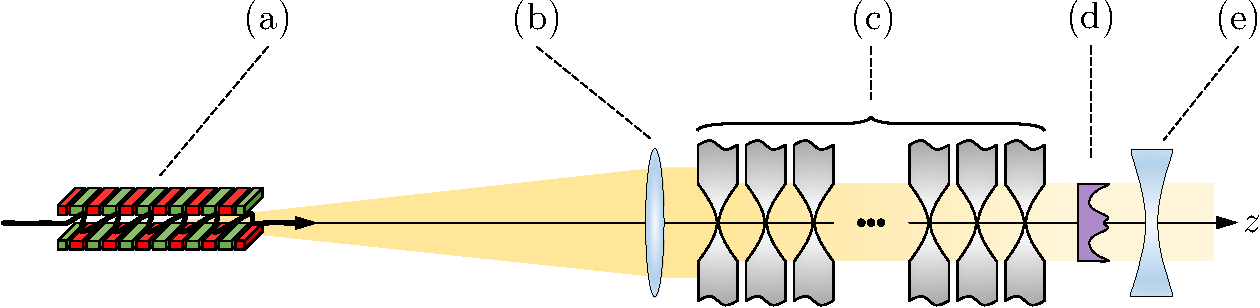
\includegraphics[width=0.6\linewidth]{figures/ch06/recovered_phase_corrected.pdf}}
        \caption[Schematic for residual thickness error calculation after phase correction]{Schematic for residual thickness error calculation after phase correction. (a) shows an arbitrary X-ray source. An (b) ideal parabolic phase element is placed downstream the radiation source to give the illumination a plane phase. The stacked X-ray lenses are placed immediately downstream. Any changes to the wave-field after (c) can be directly attributed to the model under study. The phase plate is placed in (d) to correct the accumulated phase errors. An (e) ideal parabolic phase element with a radius of curvature matching the developed quadratic term is then added and the residues (phase errors) can be extracted.}\label{fig:recovered_phase_corrected}
\end{figure}

\begin{figure}[t]
        \centering
        {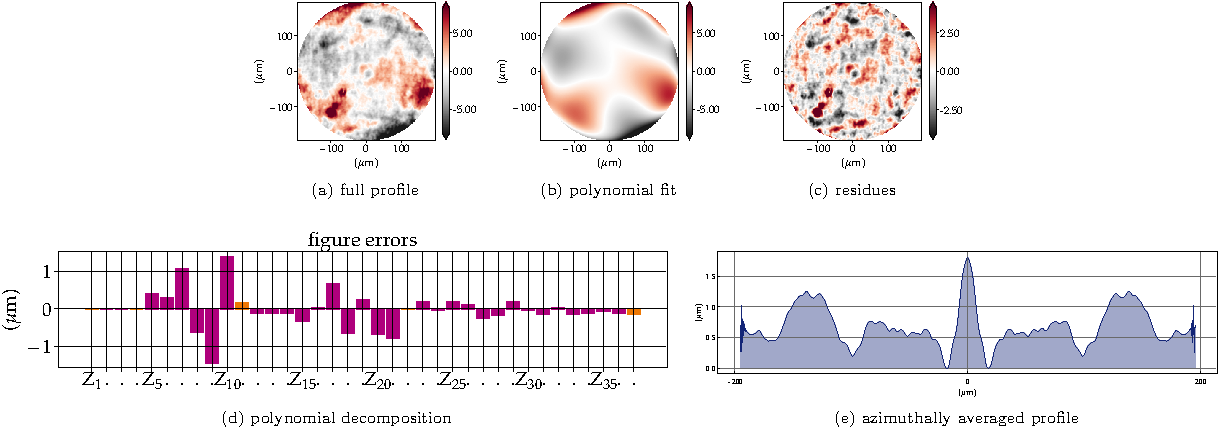
\includegraphics[width=1\linewidth]{figures/ch06/residual_profile.pdf}}
        \caption[Residual profile after phase correction]{Residual thickness error of the individually measured and artificially stacked lenses L01-L10 corrected with the diamond phase plate displayed in Fig.~\ref{fig:plate_profile}.}\label{fig:residual_profile}
\end{figure}

\begin{table}[h]
    \caption[Residual figure error profile r.m.s. value for L01-L10 and for the corrected system]{Residual figure error profile r.m.s. value for L01-L10 (Fig.~\ref{fig:accumulated_profile_1}) and for the corrected system (Fig.~\ref{fig:residual_profile}).}
    \centering
    \label{tab:corrected}\small
    \begin{tabular}{rccc}
    \hline \hline
    &\multicolumn{3}{c}{figure errors$^\dagger$ (r.m.s) $\mu$m}\\ \cline{2-4}
    &full profile & pol. fit   & residues \\ \hline
    L01-L10:      &4.84  &4.36  &2.18\\
    L01-L10 + PP: &3.27  &2.84  &1.63\\
    \hline \hline
    \multicolumn{4}{r}{\footnotesize{$^\dagger$ values given for $A_{\diameter}=400~\mu\text{m}$}}     
    \end{tabular}
\end{table}

\begin{table}[h]
    \caption[Strehl ratio for L01-L10 and for the corrected system]{Comparison of the Strehl ratio for aberrated system composed of L01-L10 and the corrected system as shown in Fig.~\ref{fig:Strehl_correction}.}\label{tab:Strehl_corrected}%\small
    \resizebox{\columnwidth}{!}{
    \centering
    \begin{tabular}{lrcccccc}\hline \hline
    &    &$\sigma_z$ ($\mu$m)     &$S_{\text{a}}$ (Eq.~\ref{eq:Strehl})  &$S_{\text{b}}$  (Eq.~\ref{eq:Marechal}) &$S_{\text{c}}$  (Eq.~\ref{eq:Mahajan}) &$S_{\text{ratio coh.}}$ &$S_{\text{ratio part.-coh.}}$ \\ \hline
    Fig.~\ref{fig:Strehl_correction} &L01-L10  &4.84  &0.067      &0.285 &0.393  &0.394         &0.409 \\
    &L01-L10 + PP                              &3.27  &0.503      &0.545 &0.608  &0.595         &0.671\\
    \hline \hline
    \end{tabular}
    }
\end{table}{}

%-------------------------------------------------------------------------
%-------------------------------------------------------------------------
\subsubsection*{Expected performance}
%-------------------------------------------------------------------------
%-------------------------------------------------------------------------

By reproducing the simulations from \S\ref{sec:coherent_sim}~-~\textit{\nameref{sec:coherent_sim}} and \S\ref{sec:partcoherent_sim}~-~\textit{\nameref{sec:partcoherent_sim}} to the corrected optical system as shown in Fig.~\ref{fig:optical_setups_corrected}, it is possible to evaluate the correction plate performance and predict its effect in a coherent- and partially-coherent X-ray beam. Figure~\ref{fig:CDn_corrected} summarises the simulations and can be directly compared to Fig.~\ref{fig:CDnS} as it
shows the beam profile at selected positions up- and downstream the focal plane for a (a) partially- and for a (b) coherent beam. The beam caustic is shown in Fig.~\ref{fig:CDn_corrected}(c), while the (d) phase and (e) amplitude of the PSF, as well as the (f) source image, are shown right next to it. A graphical representation of the Strehl ratio for the aberrated system and corrected system is shown in Fig.~\ref{fig:Strehl_correction} for the coherent and partially-coherent cases.

\begin{figure}[t]
        \centering
        {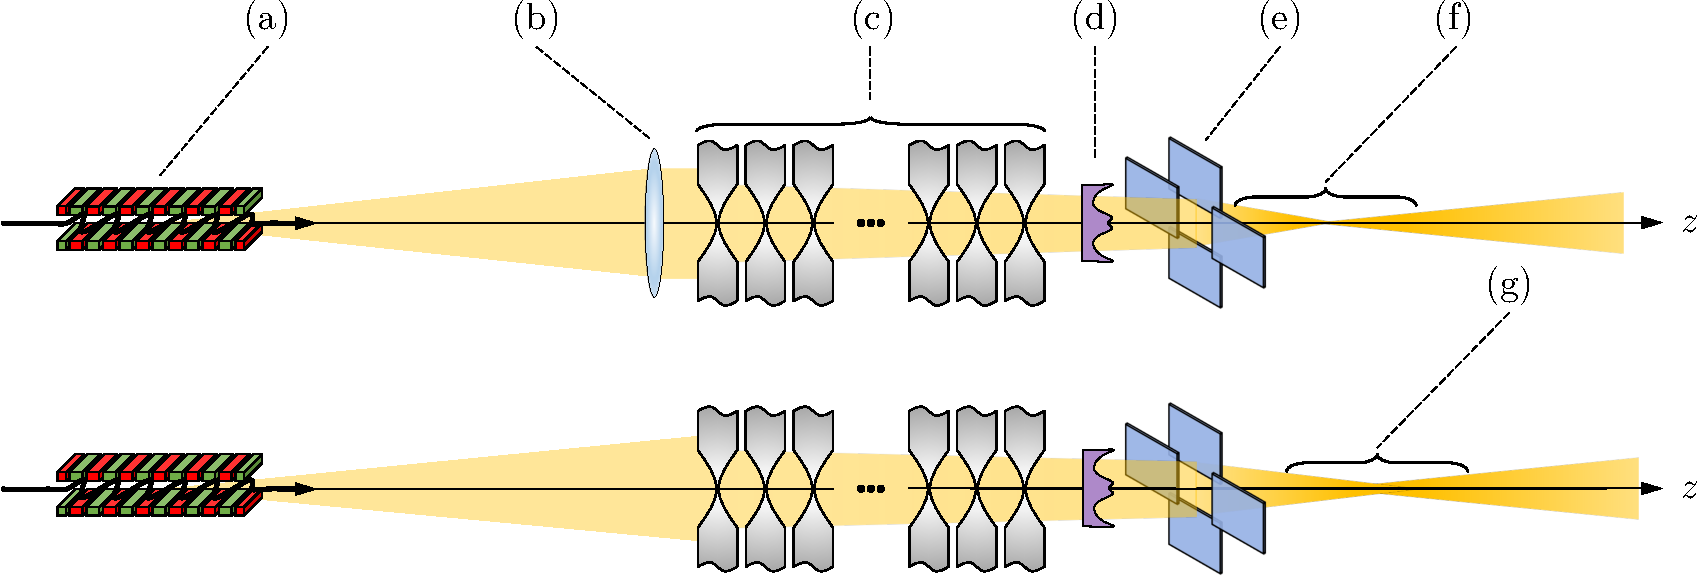
\includegraphics[width=0.8\linewidth]{figures/ch06/optical_setups_corrected.pdf}}
        \caption[Beamlines for coherent- and partially-coherent simulations]{\textbf{top row}: beamline used for  \S\ref{sec:coherent_sim}~-~\textit{\nameref{sec:coherent_sim}}. \textbf{bottom row}: beamline used for  \S\ref{sec:partcoherent_sim}~-~\textit{\nameref{sec:partcoherent_sim}}. (a) shows the X-ray source. An (b) ideal parabolic phase element is placed downstream the radiation source to give the illumination plane phase. This ideal element is only present for the fully-coherent simulations. The lenses being studied are shown in (c), which are followed by the (d) the correction plate. A set of (e) slits to ensure the same geometric aperture for all simulations. For the fully-coherent simulations, the beam-caustic range is shown in (f) and the PSF is calculated at the centre of it. For the partially-coherent simulations, the beam profile evolution along the optical axis is shown in (g) and the beam characteristics at the focal position are calculated at its centre. 
        }\label{fig:optical_setups_corrected}
\end{figure}

\begin{figure}[h]
        \centering
        {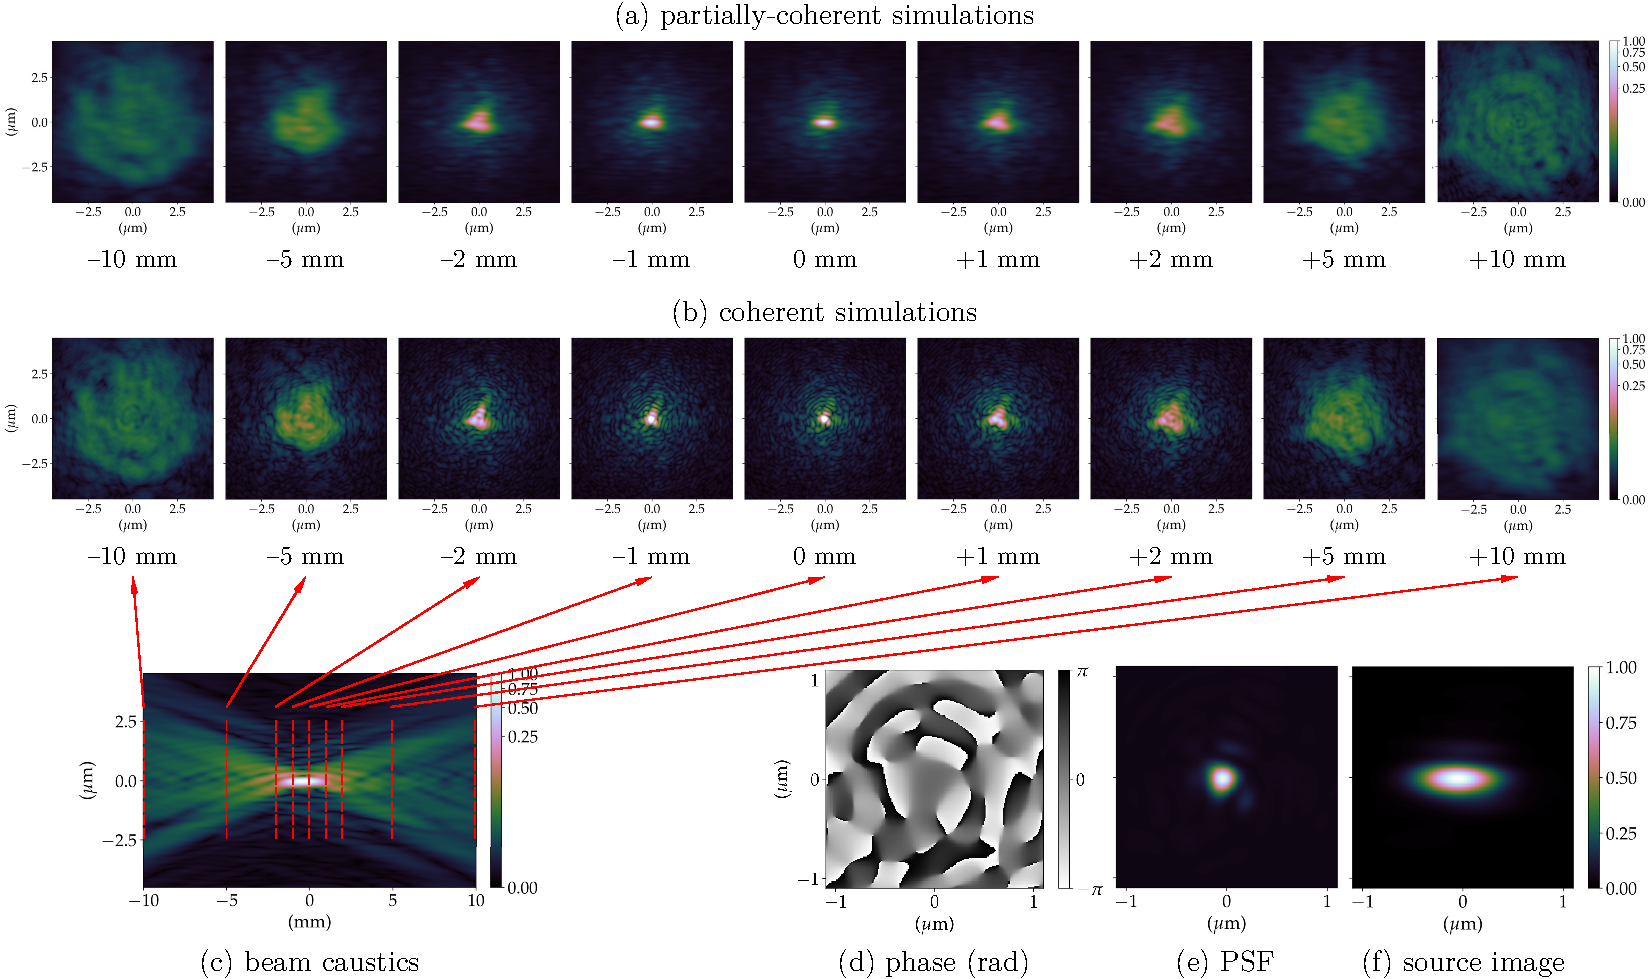
\includegraphics[width=0.99\linewidth]{figures/ch06/CDn_corrected.pdf}}
        \caption[Expected performance of the diamond phase corrector]{Expected performance of the diamond phase corrector. (a) partially-coherent simulations show the beam profile up- and downstream the focal position averaging 10$^{4}$ wavefronts to simulate the radiation emitted by an undulator; (b) the coherent simulations show the beam profile of a plane wavefront being focused; (c) beam propagation near the focal position (beam caustics) for a fully coherent beam (horizontal cut around $y=0$); (d) phase and (e) intensity of the PSF calculated focusing a plane-wavefront; (f) demagnified image of the undulator photon-source (extended source). The phase-plate was designed in diamond and a cut is shown in Fig.~\ref{fig:recovered_phase_corrected}. The residual error profile after the correction is shown in Fig.~\ref{fig:plate_profile}.}\label{fig:CDn_corrected}
\end{figure}

\begin{figure}[h]
        \centering
        {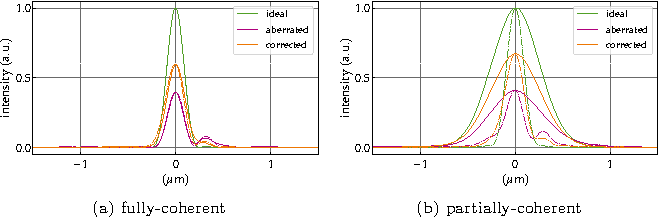
\includegraphics[width=0.7\linewidth]{figures/ch06/Strehl_correction.pdf}}
        \caption[Strehl ratio for the corrected system]{Visual representation of the Strehl ratio for the aberrated and corrected optical system. Coherent simulations are shown in (a) and partially-coherent simulations in (b) at 8~keV.}\label{fig:Strehl_correction}
\end{figure}

%-------------------------------------------------------------------------
%-------------------------------------------------------------------------
\subsubsection*{Tolerancing\footnote{This section came to be after some discussions with Andreas Schropp and Frank Seiboth (DESY, Germany) on the phase plate sensitivity to the alignment precision.}}
%-------------------------------------------------------------------------
%-------------------------------------------------------------------------

The expected performance of the correction plate shown in Figs.~\ref{fig:CDn_corrected} and \ref{fig:Strehl_correction} and compiled in the Tables~\ref{tab:corrected} and \ref{tab:Strehl_corrected} always assumes that the phase plate is perfectly centred in respect to the optical axis, at the designed distance $\Delta_{z_\text{pp}}$ from the CRL and that it presents no tilt in relation to the optical axis. However, when mounting the phase-plate in a real experimental setup, these are very difficult to reproduce. To understand and establish the precision to which the alignment has to be done, a series of scans is presented in Fig.~\ref{fig:tolerancing}, which shows the simulations of a (a) longitudinal, a (b) transverse and an angular scan of the phase plate around its nominal (designed) position. The transverse alignment is clearly very important. The longitudinal alignment is, to a lesser extent, also important. The plate shows a relative insensitivity to angular misalignments. Although Fig.~\ref{fig:tolerancing} shows only coherent simulations, it is believed that the results can be applied to a moderately partially-coherent X-ray beam without great loss.

\begin{figure}[h]
        \centering
        {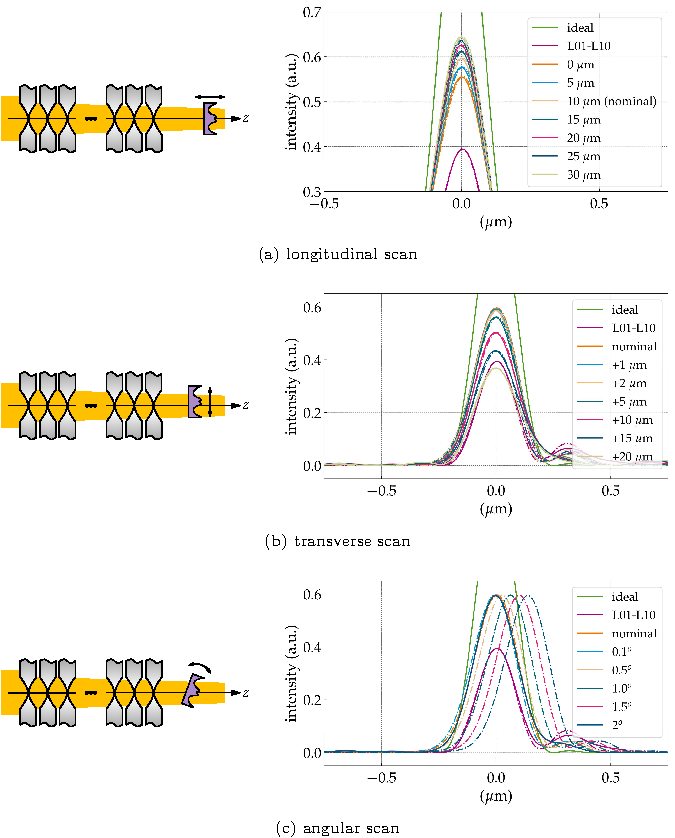
\includegraphics[width=0.7\linewidth]{figures/ch06/sensitivity_test.pdf}}
        \caption[Alignment sensitivity scan for the corrected system]{Study of the precision requirements on longitudinal, transverse and angular alignment of the phase plate based on the optimisation of the Strehl ratio for a fully-coherent beam.}\label{fig:tolerancing}
\end{figure}

\clearpage
%-------------------------------------------------------------------------
%-------------------------------------------------------------------------
\section{Prototype}\label{sec:prototype}
%-------------------------------------------------------------------------
%-------------------------------------------------------------------------

A series of phase plates designed to correct the accumulated figure error of 10 Be lenses (L01-L10) was commissioned based on the profile shown in Fig.~\ref{fig:plate_profile}, which was calculated to be placed 10~mm downstream the last lens of the stack and to correct the errors at 8~keV. The plates were ablated from diamond (HPHT IIb) by a femtosecond laser (515~nm, 3~W, 60~kHz, 200~fs) by a third-party company. The refractive phase plates produced by such technique have a surface roughness of $\sim$700~nm, but the company offers polishing, which lowers the surface roughness down to $\sim$100~nm, at the expense of removing some high-spatial frequency features of the correctors, but it is possible to account for the uneven material removal during polishing on the design of the phase plate\footnote{At the time of this writing this has not yet been tested.} [\cite{Antipov2020}]. Regardless of the surface finishing, a high shape fidelity to the profile in Fig.~\ref{fig:plate_profile} is expected from the prototypes. Lastly, to facilitate the use of the phase correctors, it was requested that the phase plates come in frames compatible with those used for X-ray lenses - see Fig.~\ref{fig:potpourri}. The phase-plate should be precisely centred in the $\diameter=12$~mm aluminium-bronze disk, so it can be easily installed in the lens housing minimising the performance degradation from misalignments shown in Fig.~\ref{fig:tolerancing}.

\begin{figure}[t]
        \centering
        {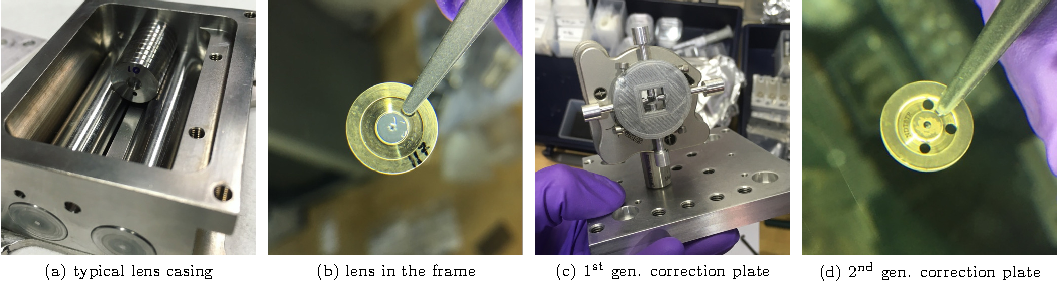
\includegraphics[width=1\linewidth]{figures/ch06/ppr.pdf}}
        \caption[Lens casing, frame and correction plates]{Typical lens casing, lens frame and both generation of correction plates. }\label{fig:potpourri}
\end{figure}
%-------------------------------------------------------------------------
%-------------------------------------------------------------------------
\subsection{Early tests on an X-ray beam}\label{sec:prototype_testing}
%-------------------------------------------------------------------------
%-------------------------------------------------------------------------

So far, only two generations of correction plates were produced - see Fig.~\ref{fig:potpourri}. The first generation of phase-plates was received and measured in Dec. 2019 with the XSVT technique described in \S\ref{sec:measuring}~-~\textit{\nameref{sec:measuring}}. This first iteration did not aim to produce useful plates, but it allowed to gain useful insights for the production of the second generation correctors, which was delivered in June 2020 - this time to be used for correction of optical imperfections in real CRLs. The phase-plates from the second generation design were chosen to demonstrate some of the preliminary results correcting optical imperfections in refractive lenses available at the ESRF.

The second generation of phase plates consisted of a set of three correction plates (PP01.v1 to PP01.v3) based on the design shown in Fig.~\ref{fig:plate_profile}. The difference among the three plates is the script used for laser ablation and the presence or not of surface post-processing. The v1 refers to an undisclosed laser polishing, while v2 and v3 have no post-processing. The PP01.v3 plate uses a different script for surface removal [\cite{Antipov2020}]. Figure~\ref{fig:pps} shows the retrieved profile using the XSVT technique and experimental setup described in \S\ref{sec:measuring}~-~\textit{\nameref{sec:measuring}}. The profiles are very similar among each other and no strong effect in the surface shape of the polished phase-plate can be observed with XSVT. For the phase-plate PP01.v2, the manufacturer provided visible light metrology (scanning confocal laser microscopy), which is shown in Fig.~\ref{fig:pp2_visible}. The surface roughness of the non-polished plate is evident in Fig.~\ref{fig:pp2_visible}(c). Figure~\ref{fig:metrology_comp} shows a profile cut of the retrieved thicknesses measured with XSVT and visible-light metrology against the designed profile, showing a initial good agreement for the central part of the phase plate and lesser agreement towards the edge of the geometric aperture.  

Once measured individually, the phase plates were added directly to the lens casing relying on the assumption that the phase-plates were perfectly centred within their frames and thus, would ideally be perfectly aligned to the lens stack - see Fig.~\ref{fig:potpourri}. The lens stack with the correction plate was then re-measured with the XSVT. For comparison, the lens stack without any correction was also measured under the very same conditions. The metrology is shown in Fig.~\ref{fig:alignment_xsvt} and summarised in Table~\ref{tab:corrected_xsvt}. It is evident that the correction plates are not centred within the lateral tolerance defined by Fig.~\ref{fig:tolerancing}(c)-(d) as no significant improvement in the residual profile can be seen.

\begin{table}[t]
    \caption[Residual figure error profile r.m.s. value for L01-L10 and for the corrected system]{Residual figure error profile r.m.s. value for L01-L10 (Fig.~\ref{fig:accumulated_profile_1}) and for the corrected system (Fig.~\ref{fig:residual_profile}).}
    \centering
    \label{tab:corrected_xsvt}\small
    \begin{tabular}{rccc}
    \hline \hline
    &\multicolumn{3}{c}{figure errors$^\dagger$ (r.m.s) $\mu$m}\\ \cline{2-4}
    &full profile & pol. fit   & residues \\ \hline
    stack 01:           &4.89  &4.73  &1.41\\
    stack 01 + PP01.v1: &3.03  &2.91  &1.66\\
    stack 01 + PP01.v2: &4.26  &3.95  &1.51\\
    stack 01 + PP01.v3: &3.44  &3.10  &1.44\\
    % stack 01 + PP02.v1: &4.86  &4.81  &1.78\\
    % stack 01 + PP02.v2: &4.09  &3.84  &1.33\\
    % stack 01 + PP02.v3: &3.59  &3.34  &1.21\\
    \hline \hline
    \multicolumn{4}{r}{\footnotesize{$^\dagger$ values given for $A_{\diameter}=320~\mu\text{m}$}}     
    \end{tabular}
\end{table}

To be able to test the correction effectiveness and performance, it was decided to mount a phase-plate outside the lens case so at least the transverse alignment could be done. The phase-plate chosen for these tests was the PP01.v2 due to its good agreement with he designed profile in Fig.~\ref{fig:plate_profile}. The simplest alignment of the phase plate is based on maximising the peak intensity at the image plane. This approach, however, could not be employed due to the saturation of the detector at the image plane even after a set of attenuators was used. Instead, the alignment of the phase-corrector was done trying to visually optimise, in terms of homogeneity, the far-field beam-profile several tens of millimetres downstream the focal plane. Once the best transverse position was found, a series of 2D images up- and downstream the optical axis was taken with the same 2D imaging detector used for the XSVT (pixel size of $\sim$0.63~$\mu$m). The beam caustics can be obtained from this series of images and it is shown in Fig.~\ref{fig:experimental_CDn_pp} for the aberrated and corrected system. Due to the saturation in the vicinity of the focal plane, a quantitative assessment of the improvement cannot be done, however, a clear qualitative improvement on the beam profile up- and downstream the focal plane is seen.


\clearpage

\begin{figure}[t]
        \centering
        {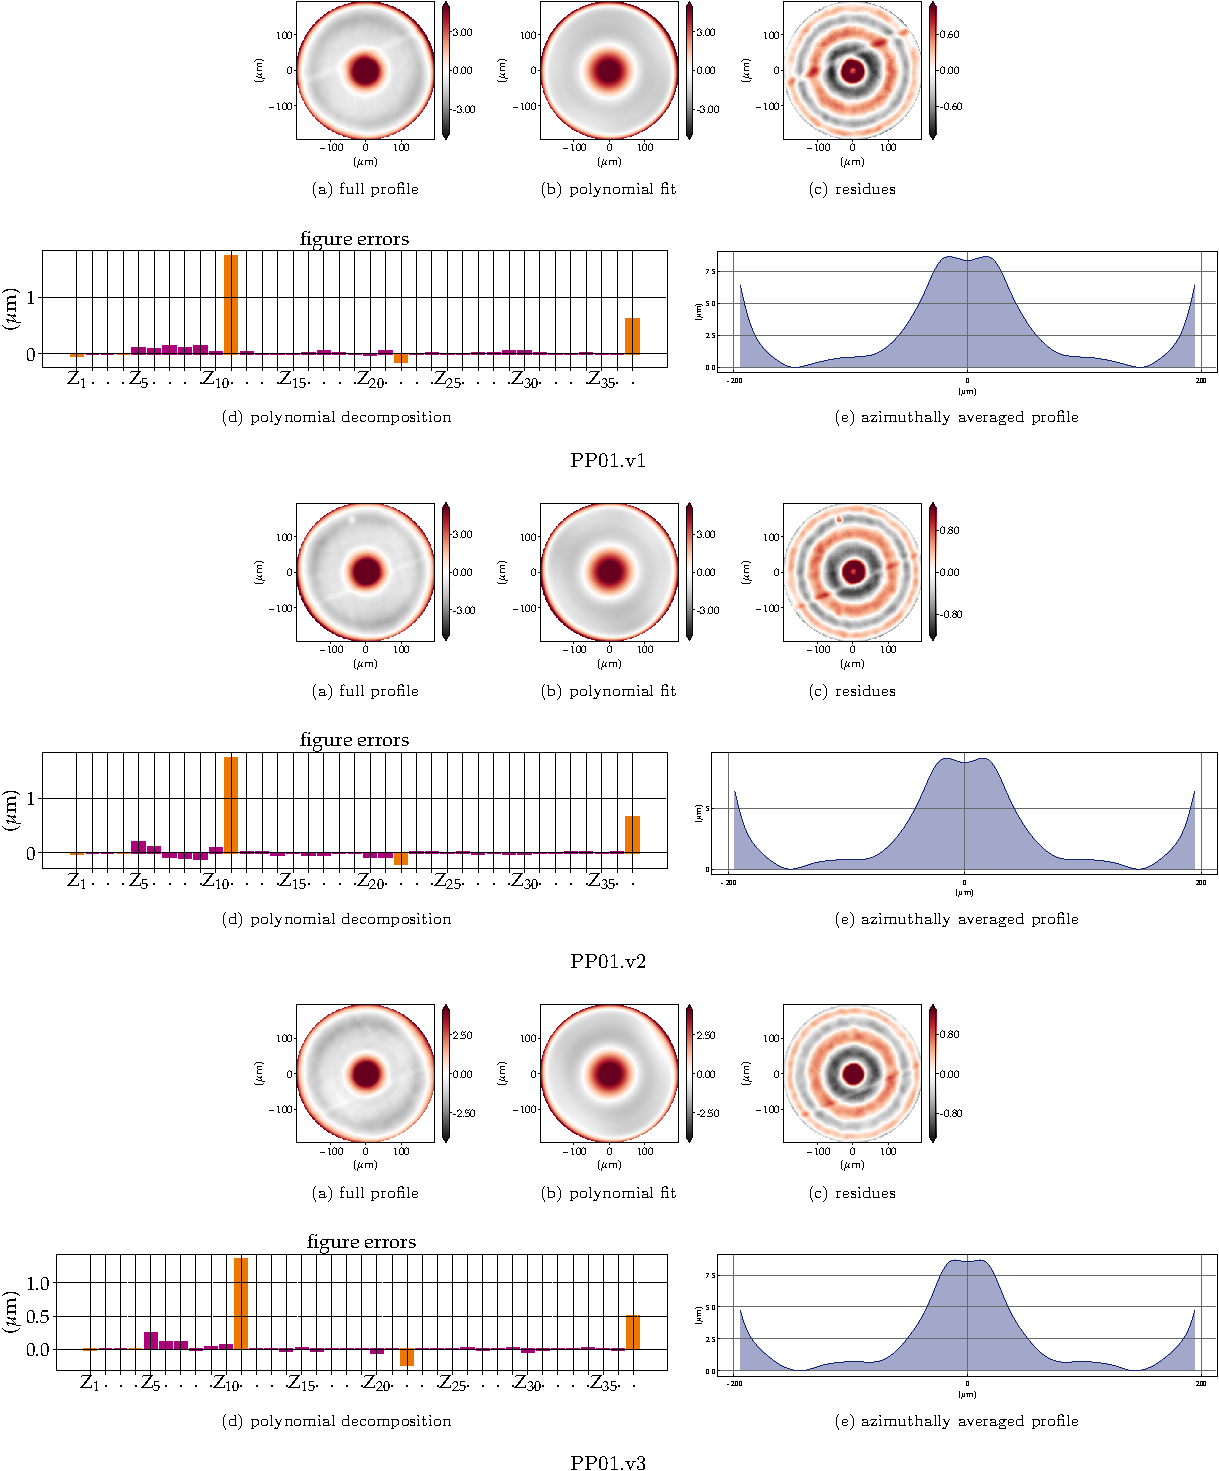
\includegraphics[width=1\linewidth]{figures/ch06/pps.pdf}}
        \caption[XSVT metrology of phase-plate PP01.v1-PP01.v3]{Phase-plate metrology using the XSVT as described in \S\ref{sec:measuring}~-~\textit{\nameref{sec:measuring}}.}\label{fig:pps}
\end{figure}

\begin{figure}[t]
        \centering
        {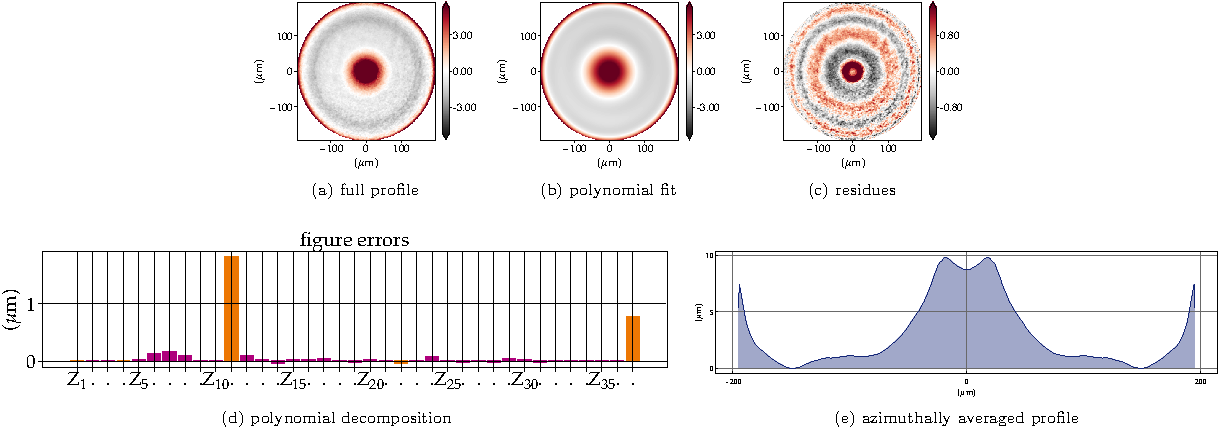
\includegraphics[width=1\linewidth]{figures/ch06/pp2_visible.pdf}}
        \caption[Scanning confocal laser microscopy of PP01.v2 phase-plate]{Scanning confocal laser microscopy of the PP01.v2 phase-plate provided by the manufacturer.}\label{fig:pp2_visible}
\end{figure}

\begin{figure}[t]
        \centering
        {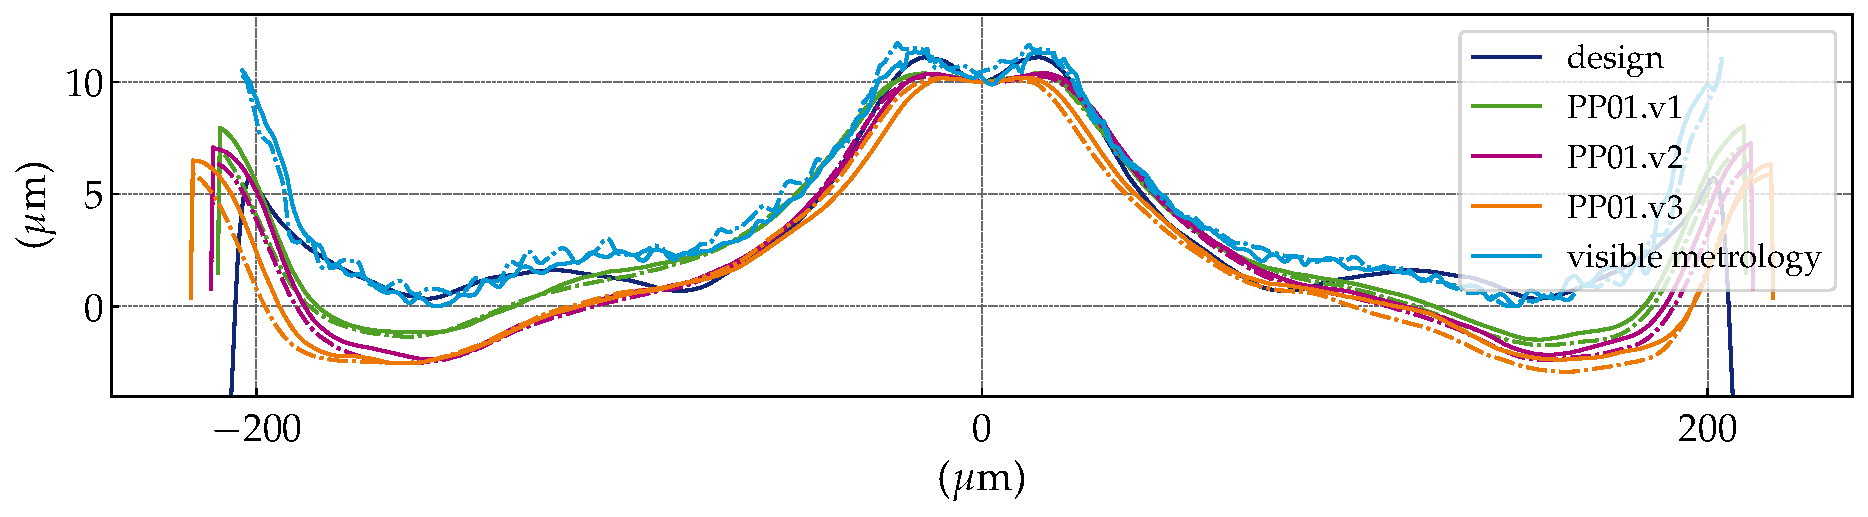
\includegraphics[width=0.7\linewidth]{figures/ch06/metrology_comp.pdf}}
        \caption[Profile cuts of the correction plates]{Profile cuts of the correction plates P01.v1-v3 measured with the XSVT metrology and from the P01.v2 plate measured with the visible-light metrology. }\label{fig:metrology_comp}
\end{figure}

\begin{figure}[t]
        \centering
        {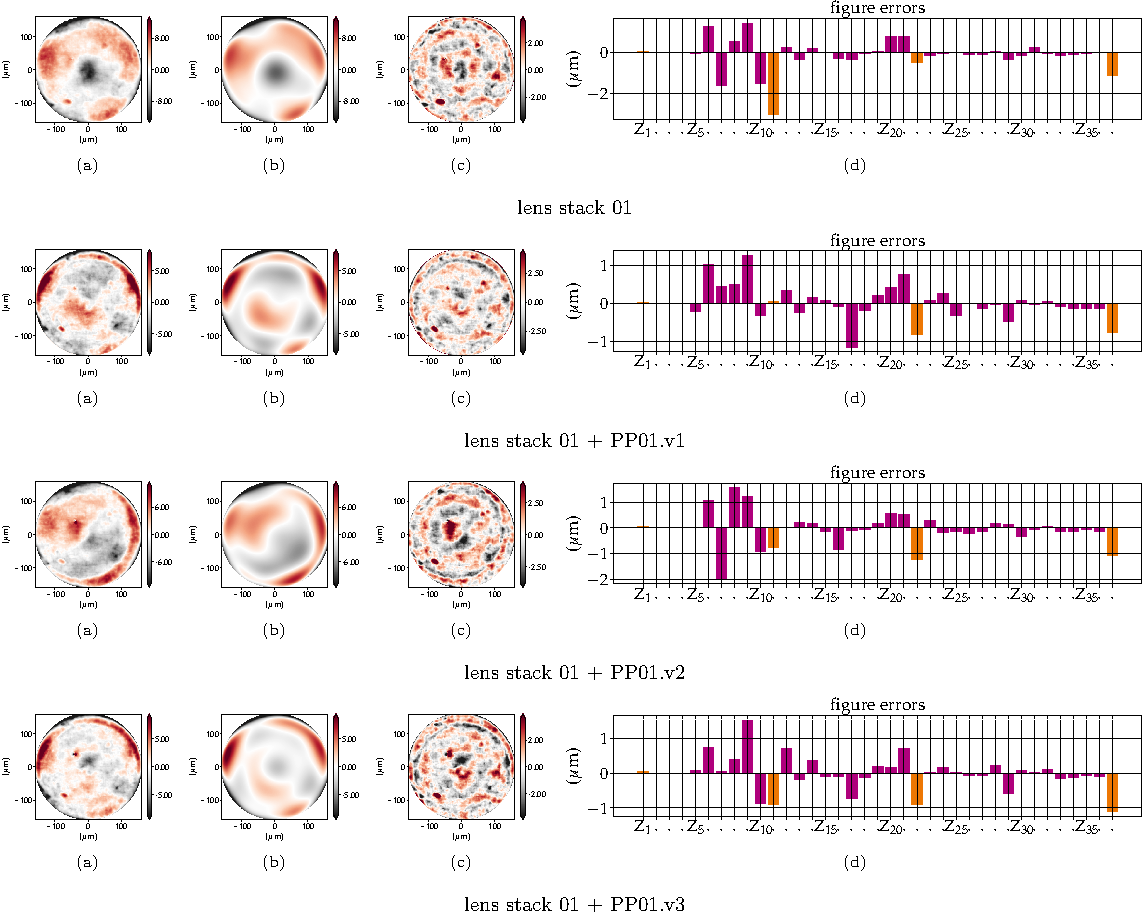
\includegraphics[width=1.0\linewidth]{figures/ch06/alignment_xsvt.pdf}}
        \caption[Residual thickness after installation of the correction plates PP01.v1-v3]{\textbf{top row}: thickness error of lens stack 01. \textbf{centre-top} to \textbf{bottom row}: residual thickness after installation of the correction plates PP01.v1, PP01.v2 and PP01.v3 respectively.}\label{fig:alignment_xsvt}
\end{figure}

\clearpage

\begin{figure}[t]
        \centering
        {\includegraphics[width=1.0\linewidth]{figures/ch06/experimental_CDn_pp.pdf}}
        \caption[Experimental beam caustics for the aberrated and corrected systems]{Experimental beam caustics taken at 10.6~keV for the aberrated and corrected system.}\label{fig:experimental_CDn_pp}
\end{figure}
%-------------------------------------------------------------------------
%-------------------------------------------------------------------------
\section{Discussion}\label{sec:corrective_optics_discussion}
%-------------------------------------------------------------------------
%-------------------------------------------------------------------------

\subsection{Design and expected performance}

The concept and design of optical correction for the aberrated system are quite simple and can be represented by the Eq.~\ref{eq:phase_plate}. Although current micro- and nano-manufacturing techniques can reproduce such intricate profiles, its alignment on a beamline can be cumbersome and render the correction plate impractical. A successful compromise for 2D focusing CRLs is the adoption of a radially symmetric correction plate described by Eq.~\ref{eq:phase_plate_r} - these have been demonstrated to work by other groups [\cite{Seiboth2017,Seiboth2018,Seiboth2020,Dhamgaye2020}]. 

Using the approach guided by Eq.~\ref{eq:phase_plate_r}, a design to compensate for the accumulated errors from lenses L01-L10 (see  Fig.~\ref{fig:accumulated_profile_1}) was calculated and it is shown in Fig.~\ref{fig:plate_profile}. Placing this ideal diamond phase-plate on the simulations and extracting the residual profile allows gaining some insight into the expected performance of the corrected system. Although most, if not all spherical aberration was removed, there is still a high content on non-symmetric aberrations as shown in Figure~\ref{fig:residual_profile}(d), which will still degrade the beam focusing quality, but to a lesser extent. Figure~\ref{fig:residual_profile}(e) shows a (much reduced) residual profile, which indicates that the correction plate should be calculation over a few iterations until the azimuthally averaged profile goes below what is currently possible to be manufactured. Table~\ref{tab:corrected} shows that the overall figure error r.m.s. value over the exit pupil is reduced to $\sim$68\% of the L01-L10 figure error. The low-frequencies are more affected, being reduced to 65\% its original value. The high frequencies are reduced to 75\% of the value before the correction. This reduction in the figure errors is accompanied by an increase in the Strehl ratio as evidenced by Table~\ref{tab:Strehl_corrected} and Fig.~\ref{fig:Strehl_correction}. The improvement of the Strehl ratio for the coherent case differs from the one for the partially-coherent case. Figure~\ref{fig:Strehl} already showed a very small difference between both cases, but it was deemed to be insignificant. This difference shows the necessity of further studying the impact of the optical correction for moderate- and low-coherence systems.

The expected improvements brought by the optical correction also apply to the beam up- and down-stream the image plane as the several cuts along the beam caustics in Fig.~\ref{fig:CDn_corrected} show. The elongated tail before the image plane and the doughnut shape from Fig.~\ref{fig:CDnS} are no longer present, however, at the image plane vicinity, satellite structures are seen around the main lobe. The image plane is greatly improved for both the fully- and partially-coherent simulations with great suppression of the side lobes, showing some similarities with the beam performance predicted in Fig.~\ref{fig:simulations_HF}. In fact, the better the correction plate is, the closer the system will behave as in Fig.~\ref{fig:simulations_HF}, a result of the high-frequency profile shown in Fig.~\ref{fig:CDnHF}. The performance of very well corrected systems will be limited by the high-frequency content, which does not significantly changes the main-lobe, but significantly increases the background around it, as shown in Fig.~\ref{fig:hf_strehl_scan}.

It is important to point out that the expected performance and all previously improvements are only obtained for the perfectly aligned phase-plate. Tolerance simulations were done to narrow down the most critical degrees of freedom when aligning the phase-plate in respect to the CRL to be corrected. The longitudinal scan is a useful tool when operating the phase plate outside the design energy. Figure~\ref{fig:tolerancing}(a)-(b) shows that a longitudinal scan of a phase-plate operating at its designed energy. Bringing the plate upstream of the nominal position $\Delta_{z_\text{pp}}$ degrades its performance, but going downstream moderately improves it. This is probably due to the higher absorption towards the edge of the plate and a smaller footprint of the beam. The transverse alignment is by far the most sensitive degree of freedom and a moderate misalignment may compromise the correction, bringing the Strehl ratio to the same value the aberrated system originally had. Figure~\ref{fig:tolerancing}(c)-(d) reinforces what has been observed by other groups [\cite[Fig.~5.12]{Seiboth2016b}]. Finally, in terms of the Strehl ratio, the phase-plate is not too much influenced by the angular alignment, provided it is kept reasonably small. A tilt is introduced to the system, which laterally shifts the focused beam, but its intensity remains largely unchanged.

\subsection{Early phase plate tests on an X-ray beam}

The early tests with the second generation of phase-plate are encouraging and help delineate strategies for further development of phase correctors to be used with the CRLs. Three phase plates were produced trying to replicate the shape in Fig.~\ref{fig:plate_profile} with differences in the scripts used for engraving the diamond slab and with post polishing or not. Figures~\ref{fig:pps} and \ref{fig:pp2_visible} show a very similar profile for all three plates where the low-frequencies are well represented, but the residues from the polynomial fit show a clear limitation of XSVT in showing the difference between a polished and non-polished plate. Although the effects of polishing are noticeable in the far-field (presence of small-angle scattering and speckle), XSVT cannot show the surface roughness as visible-light metrology does - Fig.~\ref{fig:pp2_visible}. This makes the case for using complementary metrology methods for a complete characterisation of the phase-plates. When overlapping the profile cuts, as in Fig.~\ref{fig:metrology_comp}, the difference in the profiles becomes more evident. Visible light metrology and designed plate have a more similar profile, while the data collected with XSVT show lower height values towards the edges of the phase-plate. The differences may come from the processing of the phase-gradients from the XSVT, small inaccuracies when measuring the distances in the experimental setup or a difference between the tabled index of refraction/density and the real index of refraction from the plate - something similar has been speculated in [\cite[\textit{§3.2}]{Seiboth2020}] for justifying differences between design and measured phase-plates produced using IP-S resist, a much less studied material than diamond. 

One of the key aspects of the commissioned phase-plates is that they come perfectly centred in a frame compatible to the ones used for encasing X-ray lenses - Fig.~\ref{fig:potpourri}(b) and (c), which is done to circumvent the degradation in performance from the lateral misalignment in Fig.~\ref{fig:tolerancing}(c)-(d). Unfortunately, the phase plates of the current generation do not yet meet such requirements as the metrology of the CRL with the correction plates suggests - see Fig.~\ref{fig:alignment_xsvt}; improvements in the centring of the phase plates are expected from the partner company, but are also separately under way within the X-ray optics group at the ESRF. 

Aligning the phase-plate to the CRL also revealed a very important aspect: the lack of an internal protocol for alignment. Ideally, one would scan the phase-plate transversely at each position of the scan, the residual wavefront would be calculated and the minimisation of figure errors would be sought. This approach is impractical for the XSVT due to the data acquisition and processing time, not to mention the very large data-set it would generate. This highlights the necessity to re-implement speckle-tracking based on only two images (XST)\footnote{Refer to \S\ref{sec:foundation}~-~\textit{\nameref{sec:foundation}} in \S\ref{sec:measuring}~-~\textit{\nameref{sec:measuring}}.} for a fast evaluation of the figure errors at the expense of a lower spatial resolution. This technique was less frequently used within the X-ray Optics Group due to the many advantages of XSVT [\cite{Berujon2020}], but there is a necessity to use XST for a faster characterisation.

Trying to align the phase-plate by maximising the peak intensity was the next obvious step. However, these particular experiments took place at the ID06 beamline after the ESRF-EBS upgrade, an undulator beamline that naturally has a very high photon flux at the harmonics when compared to the typical emission of bending magnets\footnote{Refer to \S\ref{sec:sources}~-~\textit{\nameref{sec:sources}}.}. This increase in photon flux is welcome for the metrology but causes the imaging detector to saturate at the image plane even after attenuators were placed in the beam. As an alternative to the optimisation of the peak intensity, the qualitative improvement of the beam profile downstream the focal plane was done. The phase plate was scanned transversely while the far-field was registered. The final position of the phase plate was where the beam was more homogeneous and the doughnut shape less evident. The drawing of general guidelines for the alignment of the phase-plates and metrics to evaluate it are the topic of future work\footnote{With the resumption of the ESRF user service mode, more access to beamtime is expected. The ESRF reopened to the public on the 25$^\text{th}$ of August 2020, despite the COVID-19 pandemic [\cite{Cho2020}].}.

The beam caustics and profiles shown in Fig.~\ref{fig:experimental_CDn_pp} for the aberrated beam confirm the results from the modelling presented in the chapter~\ref{sec:effect_optical_imperfections}~-~\textit{\nameref{sec:effect_optical_imperfections}} and published in [\cite{Celestre2020}]. The presence of the tail upstream of the focal plane and the doughnut shape downstream are clearly present. A direct comparison with the simulations is not possible due to the limited caustic step and detector pixel size, but the main elements and trends are present. Once the phase-plate is inserted and aligned, an improvement in the beam profile homogeneity is seen, although quantification is not possible, due to the saturation of the detector. The central tail is reduced, although still present upstream the image plane. More remarkable is the suppression of the doughnut shape. The performance of the correction plate is better near the image plane, but that could be from the low spatial resolution of the detector. 

\begin{figure}[t]
    \centering
    {\includegraphics[width=1\linewidth]{figures/ch03/n_plate.pdf}}
    \caption[Index of refraction ratio for common phase plate materials]{(a) diamond, (b) SU-8 and (c) fused silica (SiO$_2$) refraction index decrement ratio against beryllium. Figures obtained using the \textit{xraylib} library [\cite{Brunetti2004, Schoonjans2011}].}
    \label{fig:delta_correction_plate}
\end{figure}

The experiments were conducted at 10.6~keV, while the design of the phase-plate was optimised for 8~keV. As mentioned previously, the correction plates can be used outside the designed energy if they were calculated for a modest number of lenses by shifting them along the optical axis as described by [\cite[\textit{\S6}]{Seiboth2018}]. Figure~\ref{fig:delta_correction_plate} shows the ratio of the index of refraction decrement and the $\delta$ of beryllium, which confirms an almost negligible variation over such a small energy difference. Figure~\ref{fig:delta_correction_plate} reinforces the conclusions in [\cite[\textit{\S6}]{Seiboth2018}] for commonly used phase plate materials.

The correction performance is, at the moment, far from the expected simulated performance or the reported performance from other groups [\cite{Seiboth2017,Seiboth2018,Seiboth2020,Dhamgaye2020}]. These are the performance of second-generation phase plates and with beamtime availability. Addressing the aforementioned issues with alignment, wavefront-sensing and protocols for evaluating the performance of the phase-plates, improvements in the design and fabrication of phase plates are expected.  $\blacksquare$

\addcontentsline{toc}{section}{References}
\printbibliography[heading=subbibliography]
\end{refsection}
 \cleardoublepage

% \appendix
% \renewcommand{\thechapter}{A}

\chapter{Orthonormal aberration polynomials for optical systems}
\label{sec:appendix_poly}

\section{Zernike polynomials for circular apertures}
\section{Zernike polynomials for rectangular apertures}
\section{Legendre polynomials for anamorphic systems with rectangular apertures}
\cleardoublepage
% \setcounter{chapter}{15}
\appendix
% \renewcommand{\thechapter}{P}

\chapter{Publication list}\label{sec:publications}

\section*{Journal publications}

Nash, B., Goldring , N., Edelen, J., Webb, S. and \underline{Celestre, R.}, (2020). Propagation of partially coherent radiation using Wigner functions. \textit{Submitted to Physical Review Accelerators and Beams}. 

Qiao, Z., Shi, X., \underline{Celestre, R.} and Assoufid, L. (2020). Wavelet-transform-based speckle vector tracking method for X-ray phase imaging. \textit{Optics Express}, \textbf{28}(20), 1094. 

\underline{Celestre, R.}, Berujon, S., Roth, T., Sanchez del Rio, M. and Barrett, R. (2020). Modelling phase imperfections in compound refractive lenses. \textit{Journal of Synchrotron Radiation}, \textbf{27}(2), 305–318. 

Berujon, S., Cojocaru, R., Piault, P., \underline{Celestre, R.}, Roth, T., Barrett, R. and Ziegler, E. (2020). X-ray optics and beam characterization using random modulation: experiments. \textit{Journal of Synchrotron Radiation}, \textbf{27}(2), 293–304.

Berujon, S., Cojocaru, R., Piault, P., \underline{Celestre, R.}, Roth, T., Barrett, R. and Ziegler, E. (2020). X-ray optics and beam characterization using random modulation: theory. \textit{Journal of Synchrotron Radiation}, \textbf{27}(2), 284–292.

Sanchez del Rio, M., \underline{Celestre, R.}, Glass, M., Pirro, G., Herrera, J. R., Barrett, R., da Silva, J. C., Cloetens, P., Shi, X. and Rebuffi, L. (2019). A hierarchical approach for modeling X-ray beamlines: application to a coherent beamline. \textit{Journal of Synchrotron Radiation}, \textbf{26}(6), 1887–1901.

Chubar, O. and \underline{Celestre, R.} (2019). Memory and CPU efficient computation of the Fresnel free-space propagator in Fourier optics simulations. \textit{Optics Express}, \textbf{27}(20), 28750. 

\section*{Conference proceedings}

\underline{Celestre, R.}, Chubar, O., Roth, T., Sanchez del Rio, M. and Barrett, R. (2020). Recent developments in x-ray lenses modelling with SRW. \textit{Proc. SPIE 11493, Advances in Computational Methods for X-Ray Optics V}, 11493-17.

Chubar, O., Wiegart, L., Antipov, S., \underline{Celestre, R.}, Coles, R., Fluerasu, A. and Rakitin, M. (2020).  Analysis of hard x-ray focusing by 2D diamond CRL. \textit{Proc. SPIE 11493, Advances in Computational Methods for X-Ray Optics V}, 11493-20.

Nome, R., Giles, C., \underline{Celestre, R.}, Tasca, K., Dias, C., Vescovi, R., Faria, G. and Ferbonink, G. (2018). Compact arrangement for femtosecond laser induced generation of broadband hard x-ray pulses. \textit{High-Brightness Sources and Light-Driven Interactions}, ET1B.3.

\cleardoublepage
\addcontentsline{toc}{chapter}{Self-assertion}
%************************************************
% Declaration
%************************************************
\pdfbookmark[0]{Declaration}{Declaration}
\chapter*{Self-assertion}
\label{sec:declaration}
\thispagestyle{empty}
\vspace*{\fill}
\noindent
I hereby declare that I have produced the present work independently and using no more than the mentioned literature and auxiliary means. The parts taken directly or indirectly from outside sources are identified as such. The work has so far not been presented or published in the same or similar form to any other examination body.

\smallskip


\noindent\ {Grenoble, France, 01/02/2021}

\smallskip

\begin{flushright}
	\begin{minipage}{5cm}
		\centering\thesisName
	\end{minipage}
\end{flushright}
\vspace*{\fill}

%*****************************************
%*****************************************

\clearpage
\newpage
\mbox{\thispagestyle{empty}}

\end{document}
